\documentclass{ustbthesis}

\usepackage[numbers,sort&compress]{natbib}
\usepackage{tabularx}
\usepackage{amsmath}
\usepackage{subfig} % 去掉caption相关选项，避免与类冲突
\usepackage{subfiles}
\newcommand{\figref}[1]{~\ref{#1}~}
\newcommand{\tabref}[1]{~\ref{#1}~}
\newcommand{\thickhline}{\noalign{\hrule height 0.9pt}}
\renewcommand{\arraystretch}{1.25}
\newcolumntype{C}[1]{>{\centering\arraybackslash}p{#1}}
\newcolumntype{P}[1]{>{\centering\arraybackslash}p{#1}}

% 统一链接为黑色（避免绿色引用）
\hypersetup{colorlinks=true, linkcolor=black, citecolor=black, urlcolor=black}

% 避免 fancyhdr 报告 \headheight 过小导致的编译报错（部分模板会在 \begin{document} 后重置）
\setlength{\headheight}{14pt}
\AtBeginDocument{%
	\setlength{\headheight}{14pt}%
	\addtolength{\topmargin}{-0.7pt}%
}

%%%%%%%%%%%%%%%%%%%%%%%%%%%封面信息%%%%%%%%%%%%%%%%%%%%%%%%%%%%%%%%%%
\Author{韩晓阳}
\EnglishAuthor{Xiaoyang Han}
\Title{面向云原生应用权限提升漏洞的动态防控技术研究}
\EnglishTitle{Research on Dynamic Prevention and Control Technologies for Privilege Escalation Vulnerabilities in Cloud-Native Applications}
%\Subtitle{酵母菌催化反应机理和咪唑类离子液体酸度的研究}
%\EnglishSubtitle{Mechanistic Aspects of Baker's Yeast Mediated Reduction and Measurements of Acidity of Imidazolium Ionic Liquids}
\Date{2026年 5月 1日}
\EnglishDate{May, 2026}
\College{计算机与通信工程学院}
\EnglishCollege{School of Computer and Communication Engineering}  
\Address{海淀区学院路30号}
\EnglishAddress{30 Xueyuan Road, Haidian District}
\Affiliation{北京科技大学}
\EnglishAffiliation{University of Science and Technology Beijing}
\Postcode{100083}
\City{北京}
\EnglishCity{Beijing}
\Country{中国}
\EnglishCountry{P.R.CHINA}
\StudentCode{M202310652}
\Major{计算机科学与技术}
\EnglishMajor{Computer Science and Technology}
\Direction{软件工程方向}
\EnglishDirection{Software Engineering}
\Supervisor{孙昌爱}
\EnglishSupervisor{Chang'ai Sun}
\DegreeType{学术型}
\EnglishDegreeType{Science}
\CLCNumber{}
\UDCNumber{}
\UniversityCode{10008}
\UniversityLogoFile{images/ustb.png}
\SecurityLevel{公开}
\SubmissionDate{2026 年 05月 15日}
\EnglishSubmissionDate{May 15, 2026}
%%%%%%%%%%%%%%%%%%%%%%%%%%%封面信息%%%%%%%%%%%%%%%%%%%%%%%%%%%%%%%%%%

\begin{document}

\TitlePage
\SecondPage
\ThirdPage

\pagestyle{fancy}
\setlength{\headheight}{14pt}
%% 中英文摘要
%% 中文摘要页
\begin{ChineseAbstract}
云原生应用广泛依赖 Kubernetes 生态第三方组件，过度授权、访问控制缺陷、敏感信息泄露与网络隔离缺失等多维因素叠加，使权限提升漏洞在披露到修复之间形成"补丁窗口期"，给生产环境带来持续暴露风险。统计表明，30.4\% 的云原生权限提升漏洞在披露后存在较长的攻击窗口。现有方法多侧重通用静态核查或单项检测，难以针对特定 CVE 的利用前置条件与攻击链路给出可快速落地且对业务影响可控的临时防控方案；同时，策略从分析到组装高度依赖专家经验，难以规模化复用。

针对上述问题，本文提出面向云原生权限提升漏洞的动态防控技术框架。首先，构建融合上下文的安全知识库，从开源代码仓库、CVE 公告、Issue 与 Pull Request 等多源渠道汇聚证据，经向量化索引形成可检索的结构化知识底座。其次，设计"检索增强—思维链推导—评审反馈"的多智能体协同生成流程，由安全知识智能体整理上下文、漏洞分析智能体输出结构化威胁分析、策略生成智能体分别产出监控策略与防护策略草案，并由评审优化智能体进行多轮迭代修订。最后，以有效性、无干扰性、可部署性三维质量向量对候选策略进行排名式评估与多评审聚合，形成"证据支撑—智能推理—验证交付"的闭环。为支撑工程化落地，本文实现原型系统 KPEAgent，覆盖知识库管理、策略生成与反馈优化、专家评审排序以及策略部署管理等能力。

在 2020—2025 年收集的 55 个云原生权限提升漏洞样本上开展实验评估。消融实验表明，反馈迭代机制对策略质量贡献最为显著，移除后有效性下降 79.2\%；检索增强与思维链推导亦具有正向贡献，三模块协同使完整工作流在各维度均取得最优表现。与基线方法相比，本框架生成的策略在有效性维度提升 32.5\%，可部署性维度提升 41.2\%；多评审聚合的共识排序稳定性较单一评审提升 23.7\%，且与人工评审趋势一致。典型 CVE 案例分析进一步验证了生成策略可在准入控制、RBAC 收敛、网络隔离与运行时监测等控制点快速落地，从而在补丁窗口期有效压制攻击路径并降低风险暴露面。

\ChineseKeywords{云原生安全；权限提升漏洞；补丁窗口期防控；多智能体协同；策略生成与评估}
\end{ChineseAbstract}

%% 英文摘要页
\begin{EnglishAbstract}

Cloud-native applications extensively rely on third-party components within the Kubernetes ecosystem. The interplay of excessive permissions, access-control flaws, sensitive information exposure, and insufficient network isolation often leaves privilege escalation vulnerabilities exploitable during a patch-gap between disclosure and production-ready remediation. Statistics show that 30.4\% of such vulnerabilities exhibit a prolonged attack window after disclosure. Existing approaches focus primarily on generic static checks or single-direction detection, failing to deliver CVE-specific, deployable, and low-disruption temporary mitigations; meanwhile, assembling actionable defenses still depends heavily on expert knowledge, hindering scalability.

To address these challenges, this thesis proposes a dynamic prevention-and-control framework for privilege escalation vulnerabilities in cloud-native environments. First, an evidence-grounded security knowledge base is constructed by collecting multi-source context---including open-source repositories, CVE advisories, issues, and pull requests---and organizing it via vector indexing into a retrievable structured foundation. Second, a multi-agent collaborative workflow combining retrieval-augmented generation, chain-of-thought reasoning, and iterative review feedback is designed: a security-knowledge agent consolidates context, a vulnerability-analysis agent produces structured threat reports, a policy-generation agent drafts both monitoring and protection policies, and a review-optimization agent refines candidates through multiple iterations. Third, candidate policies are evaluated using a ranking-based scheme with a three-dimensional quality vector---Effectiveness, Interference, and Deployability---followed by multi-judge aggregation to form a closed loop of ``evidence support $\rightarrow$ intelligent reasoning $\rightarrow$ verified delivery.'' A prototype system, KPEAgent, is implemented to operationalize the end-to-end workflow, covering knowledge base management, policy generation with feedback-driven refinement, expert review and ranking, and deployment management.

Experiments are conducted on 55 privilege escalation CVEs collected from 2020 to 2025. Ablation studies reveal that the feedback-iteration mechanism contributes most significantly: removing it causes effectiveness to drop by 79.2\%; retrieval augmentation and chain-of-thought reasoning also yield positive gains, and the synergy of all three modules leads to optimal performance across all dimensions. Compared with baseline methods, the proposed framework improves effectiveness by 32.5\% and deployability by 41.2\%; the consensus ranking from multi-judge aggregation is 23.7\% more stable than single-judge results and aligns well with human expert assessments. Case studies on representative CVEs further confirm that the generated policies can be rapidly deployed with common cloud-native controls---including admission control, RBAC hardening, network micro-segmentation, and runtime monitoring---to suppress attack paths and reduce exposure during the patch-gap.

\EnglishKeywords{Cloud-native security; Privilege escalation; Patch-gap defense; Multi-agent collaboration; Policy generation and evaluation}


\end{EnglishAbstract}

%% 序言
% \include{contents/preclude}
% \tableofcontents

% %% 插图清单
\chapter*{插图清单}

\begingroup
\renewcommand{\listfigurename}{插图清单}
\addcontentsline{toc}{chapter}{插图清单}
\listoffigures
\endgroup

\chapter*{附表清单}
\begingroup
\renewcommand{\listtablename}{附表清单}
\addcontentsline{toc}{chapter}{附表清单}
\listoftables
\endgroup

% 
\begingroup
\setlength{\parskip}{0.2em}

\chapter*{符号清单与术语表}\addcontentsline{toc}{chapter}{符号清单与术语表}

本文中频繁使用的主要符号、核心术语与常用缩写汇总如下。为避免与正文重复，本页重点列出第三章方法定义与后续评价分析中反复出现的记号与表述。

{\noindent\large\textbf{符号清单}\par}
\vspace{0.2em}

\noindent\textbf{基本对象与集合}

\begingroup
\small
\centering
\setlength{\tabcolsep}{3pt}
\renewcommand{\arraystretch}{1.03}
\begin{tabularx}{0.90\textwidth}{>{\centering\arraybackslash}p{2.9cm} >{\raggedright\arraybackslash}X}
\toprule
\textbf{符号} & \textbf{含义说明} \\
\midrule
$\mathcal{V}$ & 漏洞实例空间，表示全部待分析漏洞构成的集合。 \\
$v=\langle \mathit{id},d,m \rangle$ & 单个漏洞实例，由编号、描述与元数据组成。 \\
$\mathit{id}$ & 漏洞标识符，如 CVE 编号。 \\
$d$ & 漏洞描述文本，用于刻画漏洞事实。 \\
$m$ & 漏洞元数据，如严重性、受影响组件与版本范围等。 \\
$\mathcal{C}$ & 安全上下文空间，表示与漏洞相关的证据集合空间。 \\
$c$ & 安全上下文，即带来源标识的有限证据集合。 \\
$t_i$ & 第 $i$ 条证据内容，如代码片段、公告文本或文档片段。 \\
$\mathit{src}_i$ & 第 $i$ 条证据来源，如文档路径、链接或代码位置。 \\
$\Pi$ & 候选策略全集，表示所有候选监控策略与防护策略的总集合。 \\
$\pi=\langle \mathit{type},\mathit{method},\mathit{action} \rangle$ & 单个安全策略，由策略类型、控制机理与执行表达组成。 \\
$\mathit{type}$ & 策略类型，取值为监控型或防护型。 \\
$\mathit{method}$ & 控制机理序列，用于表示策略采用的控制手段。 \\
$\mathit{action}$ & 执行表达序列，对应可部署的规则、配置或命令。 \\
$\Pi_v$ & 漏洞 $v$ 的候选策略集合，由生成阶段针对漏洞 $v$ 产出。 \\
$\mathcal{T}=\{\mathrm{mon},\mathrm{prot}\}$ & 策略类型集合，分别表示监控型与防护型。 \\
$\tau$ & 类型变量，表示某一给定策略类型。 \\
$\Pi_v^{\tau}$ & 同类型候选子集，表示漏洞 $v$ 在类型 $\tau$ 下的候选集合。 \\
\bottomrule
\end{tabularx}
\endgroup

\vspace{0.35em}

\noindent\textbf{评价与聚合记号}

\begingroup
\small
\centering
\setlength{\tabcolsep}{3pt}
\renewcommand{\arraystretch}{1.03}
\begin{tabularx}{0.90\textwidth}{>{\centering\arraybackslash}p{2.9cm} >{\raggedright\arraybackslash}X}
\toprule
\textbf{符号} & \textbf{含义说明} \\
\midrule
$\Delta=\{E,I,D\}$ & 评价维度集合，分别对应有效性、无干扰性与可部署性。 \\
$q(\pi)$ & 三维质量向量，表示策略 $\pi$ 在三个维度上的质量。 \\
$E(\pi)$ & 有效性，用于衡量对主要攻击路径与关键风险面的覆盖程度。 \\
$I(\pi)$ & 无干扰性，衡量对正常业务的扰动程度及误报风险。 \\
$D(\pi)$ & 可部署性，衡量策略在现有环境中的落地难度。 \\
$\mathcal{H}$ & 评价主体集合，表示多个评审主体构成的集合。 \\
$r_{\delta}^{(h)}$ & 秩函数，表示评价主体 $h$ 在维度 $\delta$ 上给出的排序位置。 \\
$s_{\delta}^{(h)}(\pi)$ & 归一化秩得分，用于将排序位置归一化到 $[0,1]$ 区间。 \\
$\hat S_{\delta}(\pi)$ & 共识得分，表示多个评价主体在维度 $\delta$ 上的聚合结果。 \\
$U_{\delta}(\pi)$ & 分歧度量，用于刻画不同评审结果的一致性程度。 \\
$Q(\pi)$ & 总体质量函数，表示综合三维共识得分后的最终质量。 \\
$\alpha_E,\alpha_I,\alpha_D$ & 维度权重，分别对应有效性、无干扰性与可部署性的权重。 \\
\bottomrule
\end{tabularx}
\endgroup

\vspace{0.45em}

{\noindent\large\textbf{术语表}\par}
\vspace{0.2em}

为统一全文表述，本文使用频率较高的核心术语与常用缩写说明如下。

\noindent\textbf{核心术语}

\begingroup
\small
\centering
\setlength{\tabcolsep}{3pt}
\renewcommand{\arraystretch}{1.03}
\begin{tabularx}{0.90\textwidth}{>{\centering\arraybackslash}p{1.8cm} >{\centering\arraybackslash}p{3.0cm} >{\raggedright\arraybackslash}X}
\toprule
\textbf{术语} & \textbf{英文/缩写} & \textbf{说明} \\
\midrule
云原生 & Cloud-native & 本文研究对象所处的应用与基础设施环境。 \\
Kubernetes & K8s & 本文默认指 Kubernetes 容器编排平台，K8s 为其常用缩写。 \\
权限提升 & Privilege Escalation & 攻击者突破原有权限边界并获取更高权限的过程。 \\
补丁窗口期 & Patch-gap window & 漏洞披露至补丁可用或补丁完成部署之间的时间段。 \\
临时防控 & Interim mitigation & 在补丁窗口期内用于降低风险的临时控制措施。 \\
安全策略 & Security strategy & 监控策略与防护策略的上位概念。 \\
监控策略 & Monitoring strategy & 面向异常行为感知、告警与取证的策略。 \\
防护策略 & Protection strategy & 面向攻击阻断、权限收敛与攻击面控制的策略。 \\
安全上下文 & Security context & 与具体漏洞相关的证据集合及其来源标识。 \\
安全知识库 & Security knowledge base & 存放多源证据、向量索引及元数据的知识支撑体系。 \\
多智能体协同 & Multi-agent collaboration & 由多个功能角色协同完成分析、生成与评审的工作方式。 \\
检索增强 & RAG & Retrieval-Augmented Generation \\
思维链推理 & CoT & Chain-of-Thought，思维链。 \\
反馈优化 & Feedback & 基于评审结果对候选策略进行修订与收敛的过程。 \\
\bottomrule
\end{tabularx}
\endgroup

\vspace{0.35em}

\noindent\textbf{常用缩写}

\begingroup
\small
\centering
\setlength{\tabcolsep}{3pt}
\renewcommand{\arraystretch}{1.03}
\begin{tabularx}{0.90\textwidth}{>{\centering\arraybackslash}p{2cm} >{\raggedright\arraybackslash}p{4.9cm} >{\raggedright\arraybackslash}X}
\toprule
\textbf{缩写} & \textbf{英文全称} & \textbf{中文说明} \\
\midrule
CVE & Common Vulnerabilities and Exposures & 通用漏洞与暴露。 \\
CWE & Common Weakness Enumeration & 通用弱点枚举。 \\
CVSS & Common Vulnerability Scoring System & 通用漏洞评分系统。 \\
NVD & National Vulnerability Database & 国家漏洞数据库。 \\
CNCF & Cloud Native Computing Foundation & 云原生计算基金会。 \\
K8s & Kubernetes & Kubernetes 的常用缩写。 \\
RBAC & Role-Based Access Control & 基于角色的访问控制。 \\
LLM & Large Language Model & 大语言模型。 \\
\bottomrule
\end{tabularx}
\endgroup

\endgroup


\mainmatter
\pagestyle{fancy}
\setlength{\headheight}{14pt}

\chapter{引言}
本章节主要介绍课题的研究背景与意义、研究内容与成果，以及论文的组织结构。

\section{背景与意义}
容器技术通过内核级资源隔离与标准化的镜像分发机制，极大地优化了微服务应用的生命周期管理。作为容器编排领域的核心基础设施，Kubernetes 提供的分布式容器编排能力有效支撑了复杂业务的部署与扩展\cite{kubernetes2024,alibaba2024}。为满足多样化的服务治理需求，现代 Kubernetes 集群需深度集成云原生计算基金会(CNCF)开源生态中的第三方应用，各类组件通过基于角色的访问控制 (RBAC) 机制\cite{ferraiolo1995role}获取集群资源访问权限。这些第三方应用的使用在赋能业务的同时也化引入了潜在的攻击面，特别是在多租户场景下，过度权限配置\cite{yang2023take}、内部权限管理缺陷、敏感信息泄露、网络隔离缺失等多维因素可能带来权限提升风险，对云原生系统的整体安全构成系统性威胁。
\begin{figure}[htbp]
    \centering
    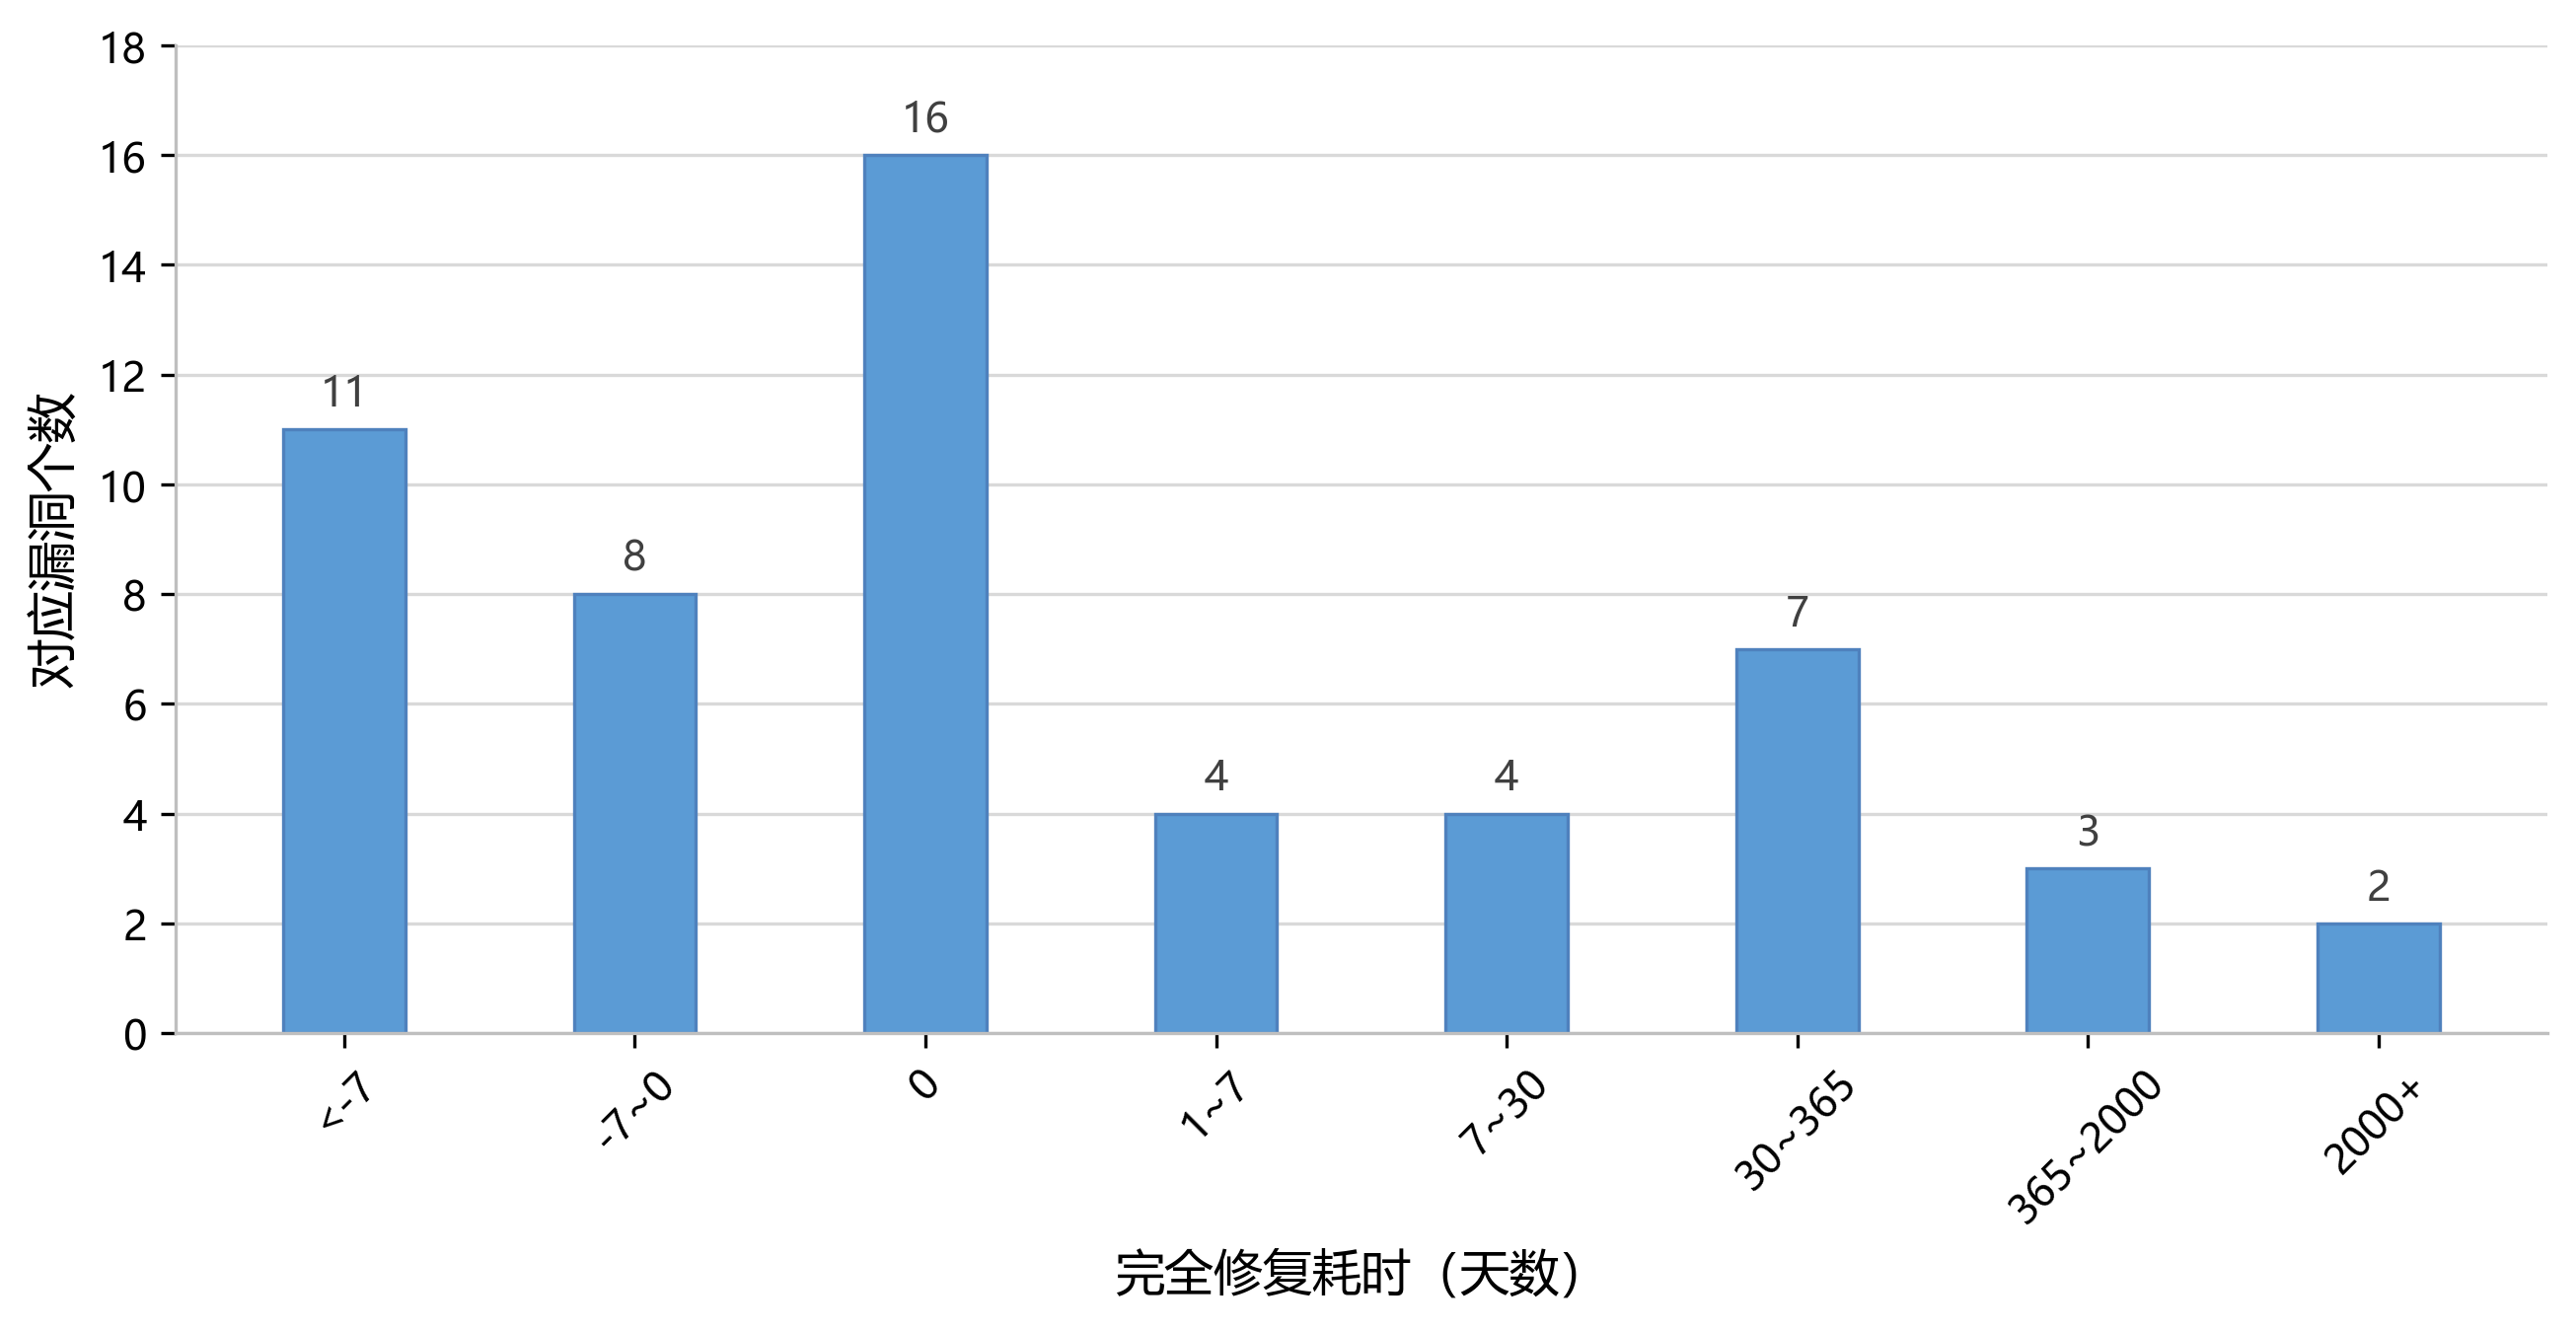
\includegraphics[width=0.8\textwidth]{images/cve-pub.png}
    \caption{云原生环境下权限提升漏洞的修复时间分布}\label{fig:patch-window}
\end{figure}

云原生第三方开源应用的权限提升漏洞从披露到修复通常面临显著的响应滞后。根据本文统计的2020年至2025年间55个云原生权限提升漏洞样本的统计，有30.4\%漏洞在披露后存在较长的攻击窗口期(见图~\ref{fig:patch-window})。开源应用官方补丁的发布、验证与分发存在相应周期管理失职会带来攻击窗口；进一步的，由于生产环境组件组合复杂且兼容性要求高，用户往往难以及时完成受影响组件的升级。在补丁尚未就绪或升级受阻的阶段，企业亟需一种可快速下发、可验证且可回滚的临时防控措施，通过压制攻击路径来降低风险暴露面。


\section{内容与成果}
基于上述现实需求，本文聚焦于云原生权限提升漏洞在补丁窗口期内的动态防控技术。通过分析漏洞公告与多维可追溯上下文，基于大语言模型构建多智能体协同的安全策略生成系统，自动化生成并筛选针对性的临时防控策略。从防控机制的作用维度考量，本文将云原生环境下的动态控制手段归纳为\textbf{监控策略}与\textbf{防护策略}两个互补层次：其中监控策略侧重运行时异常行为的感知与取证，防护策略侧重事前阻断与攻击面收敛。具体可落地控制点包括： 
\begin{itemize} 
    \item \textbf{防护策略层}：
    \begin{itemize}
        \item \textit{准入控制与配置约束}：通过 OPA/Gatekeeper\cite{opa2025} 或 Kyverno\cite{kyverno2025} 等准入控制器，在资源对象持久化前对特权容器、危险路径挂载及异常 RBAC 绑定等高风险配置实施\textbf{强制阻断}。
        \item \textit{网络隔离与连通收敛}：基于 NetworkPolicy 构建微隔离边界，将工作负载间可达性收敛至最小必要集合，从而抑制横向移动与数据外传路径。
        \item \textit{权限与配置动态加固}：面向漏洞利用路径，通过收紧 RBAC 授权边界、移除冗余权限以及调整容器运行时安全上下文，压缩攻击成功概率。
    \end{itemize}
    \item \textbf{监控策略层}：
    \begin{itemize}
        \item \textit{运行时行为监测}：基于 Falco\cite{falco2025} 等系统调用层监控工具，对异常系统调用、特权提升行为及敏感文件访问进行\textbf{实时告警与取证}，并可结合响应流程抑制影响扩散。
    \end{itemize}
    \item \textbf{防测一体工具}：
    \begin{itemize}
        \item \textit{Cilium Tetragon}\cite{tetragon2025}：基于 eBPF 的安全观测与运行时强制执行工具，兼具\textbf{监控策略}（进程执行、系统调用、I/O活动的实时检测）与\textbf{防护策略}（内核层面的策略过滤与阻断）能力，实现从感知到响应的闭环防护。
    \end{itemize}
\end{itemize}

\begin{figure}[htbp]
    \centering
    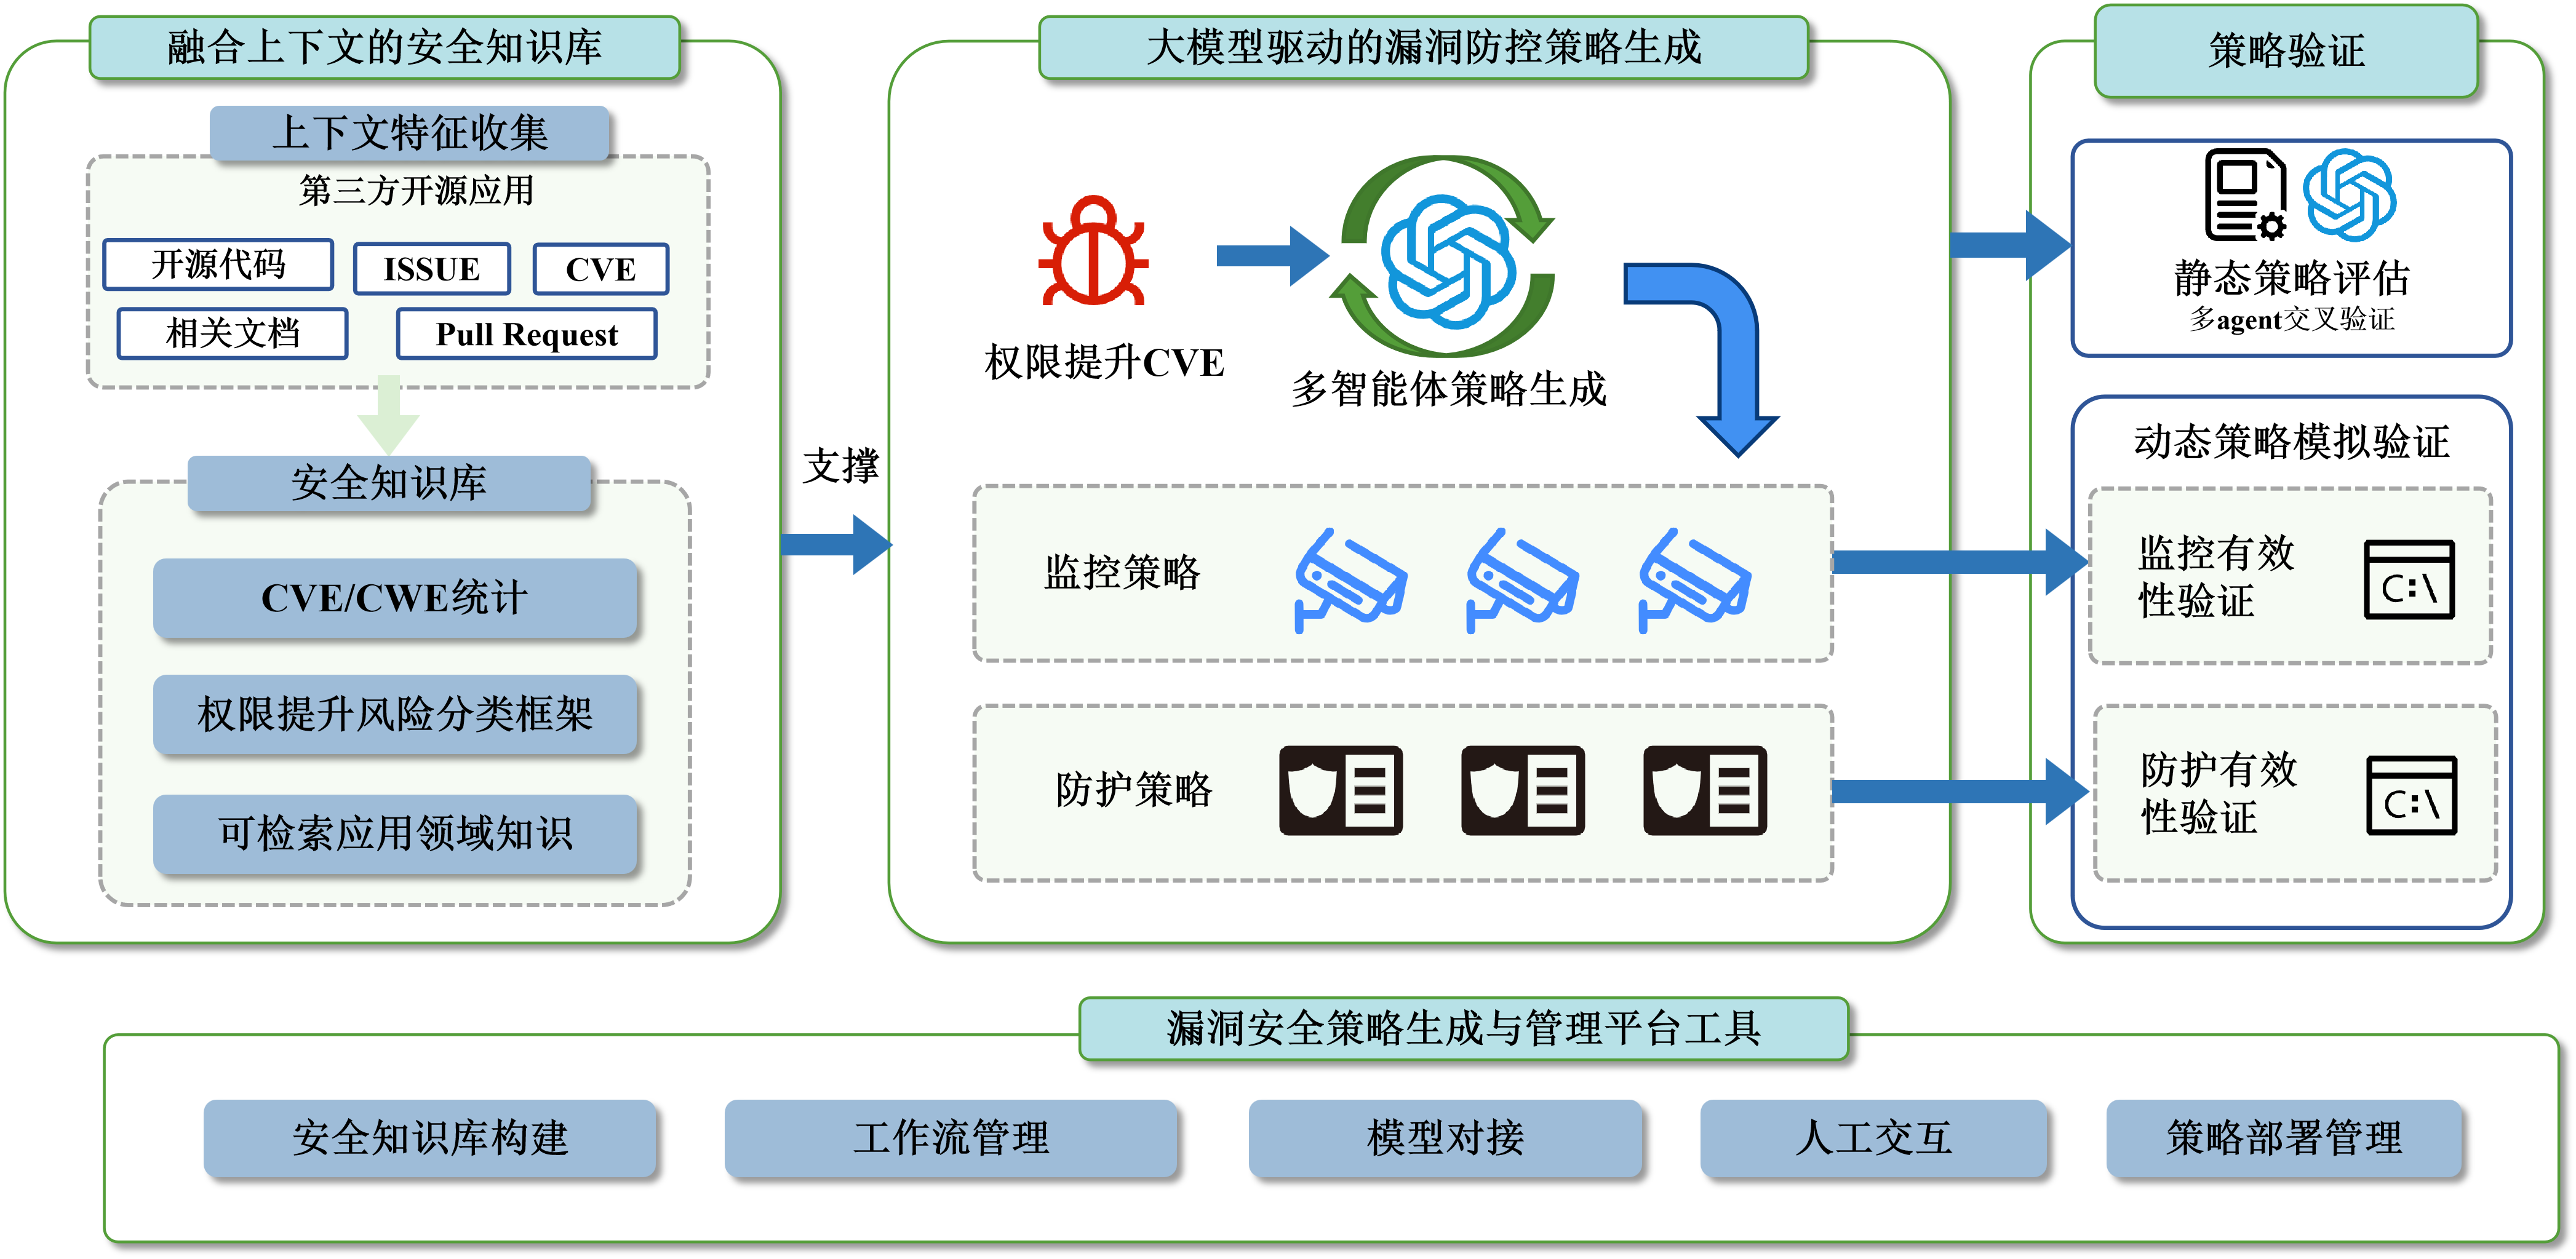
\includegraphics[width=0.98\textwidth]{images/总体框架.png}
    \caption{基于大语言模型的多 Agent 漏洞临时防控总体框架}\label{fig:overall-framework}
\end{figure}

如图~\ref{fig:overall-framework}所示，本文提出的自动化临时防控框架围绕安全知识库、策略生成与策略验证形成闭环，具体研究点包括：
\begin{itemize}
    \item \textbf{融合上下文的安全知识库构建}：面向云原生第三方开源应用场景，融合漏洞公告、开源代码与社区协作信息等多源上下文，形成可追溯的漏洞事实依据与可检索的领域知识，并沉淀面向权限提升风险成因的分类框架。
    \item \textbf{多智能体协同的防控策略生成}：以权限提升类 CVE 为输入，在知识库支持下组织多智能体协同生成候选策略集合，涵盖监控策略与防护策略两类控制目标，输出可执行的策略草案。
    \item \textbf{安全策略筛选与验证}：结合静态策略评估与动态模拟验证，对候选策略进行有效性与安全性筛选，保证策略具备可部署、可验证与可回滚的工程可用性。
    \item \textbf{平台化工具支撑}：提供知识库维护、工作流编排、模型对接与策略部署管理等能力，支撑策略生成与验证过程的持续迭代。
\end{itemize}





\section{论文组织结构}

全文结构如下：第\ref{chap:background}章介绍相关概念、技术与国内外研究现状；第\ref{chap:method}章给出面向云原生权限提升漏洞的智能防控技术体系；第\ref{chap:system}章描述漏洞防控系统设计与实现；第\ref{chap:experiment}章呈现实验设置与结果；第\ref{chap:case}章给出案例分析；第\ref{chap:conclusion}章总结与展望。

\chapter{背景介绍}\label{chap:background}
本章介绍相关概念与技术，并梳理 Kubernetes 权限提升漏洞相关的国内外研究现状。

\section{相关概念与技术}

\subsection{容器}

服务应用的部署经历从物理机部署、到虚拟机部署、再到容器化部署的演进过程（见图~\ref{fig:container-evolution}）。虚拟机部署基于KVM等虚拟化技术，实现了完整操作系统模拟与资源隔离与复用，但存在虚拟化开销较大，启动时间较长，镜像体积庞大等问题，影响了应用的交付效率和资源利用率。与传统的物理机和虚拟机相比，容器通过操作系统内核级的资源隔离，实现了更高的资源利用率和更快的启动速度。容器以\textbf{镜像}为交付单元，将部署应用及其依赖环境以镜像形式打包。容器技术原理依赖三类内核技术：
\begin{figure}[htb]
    \centering
    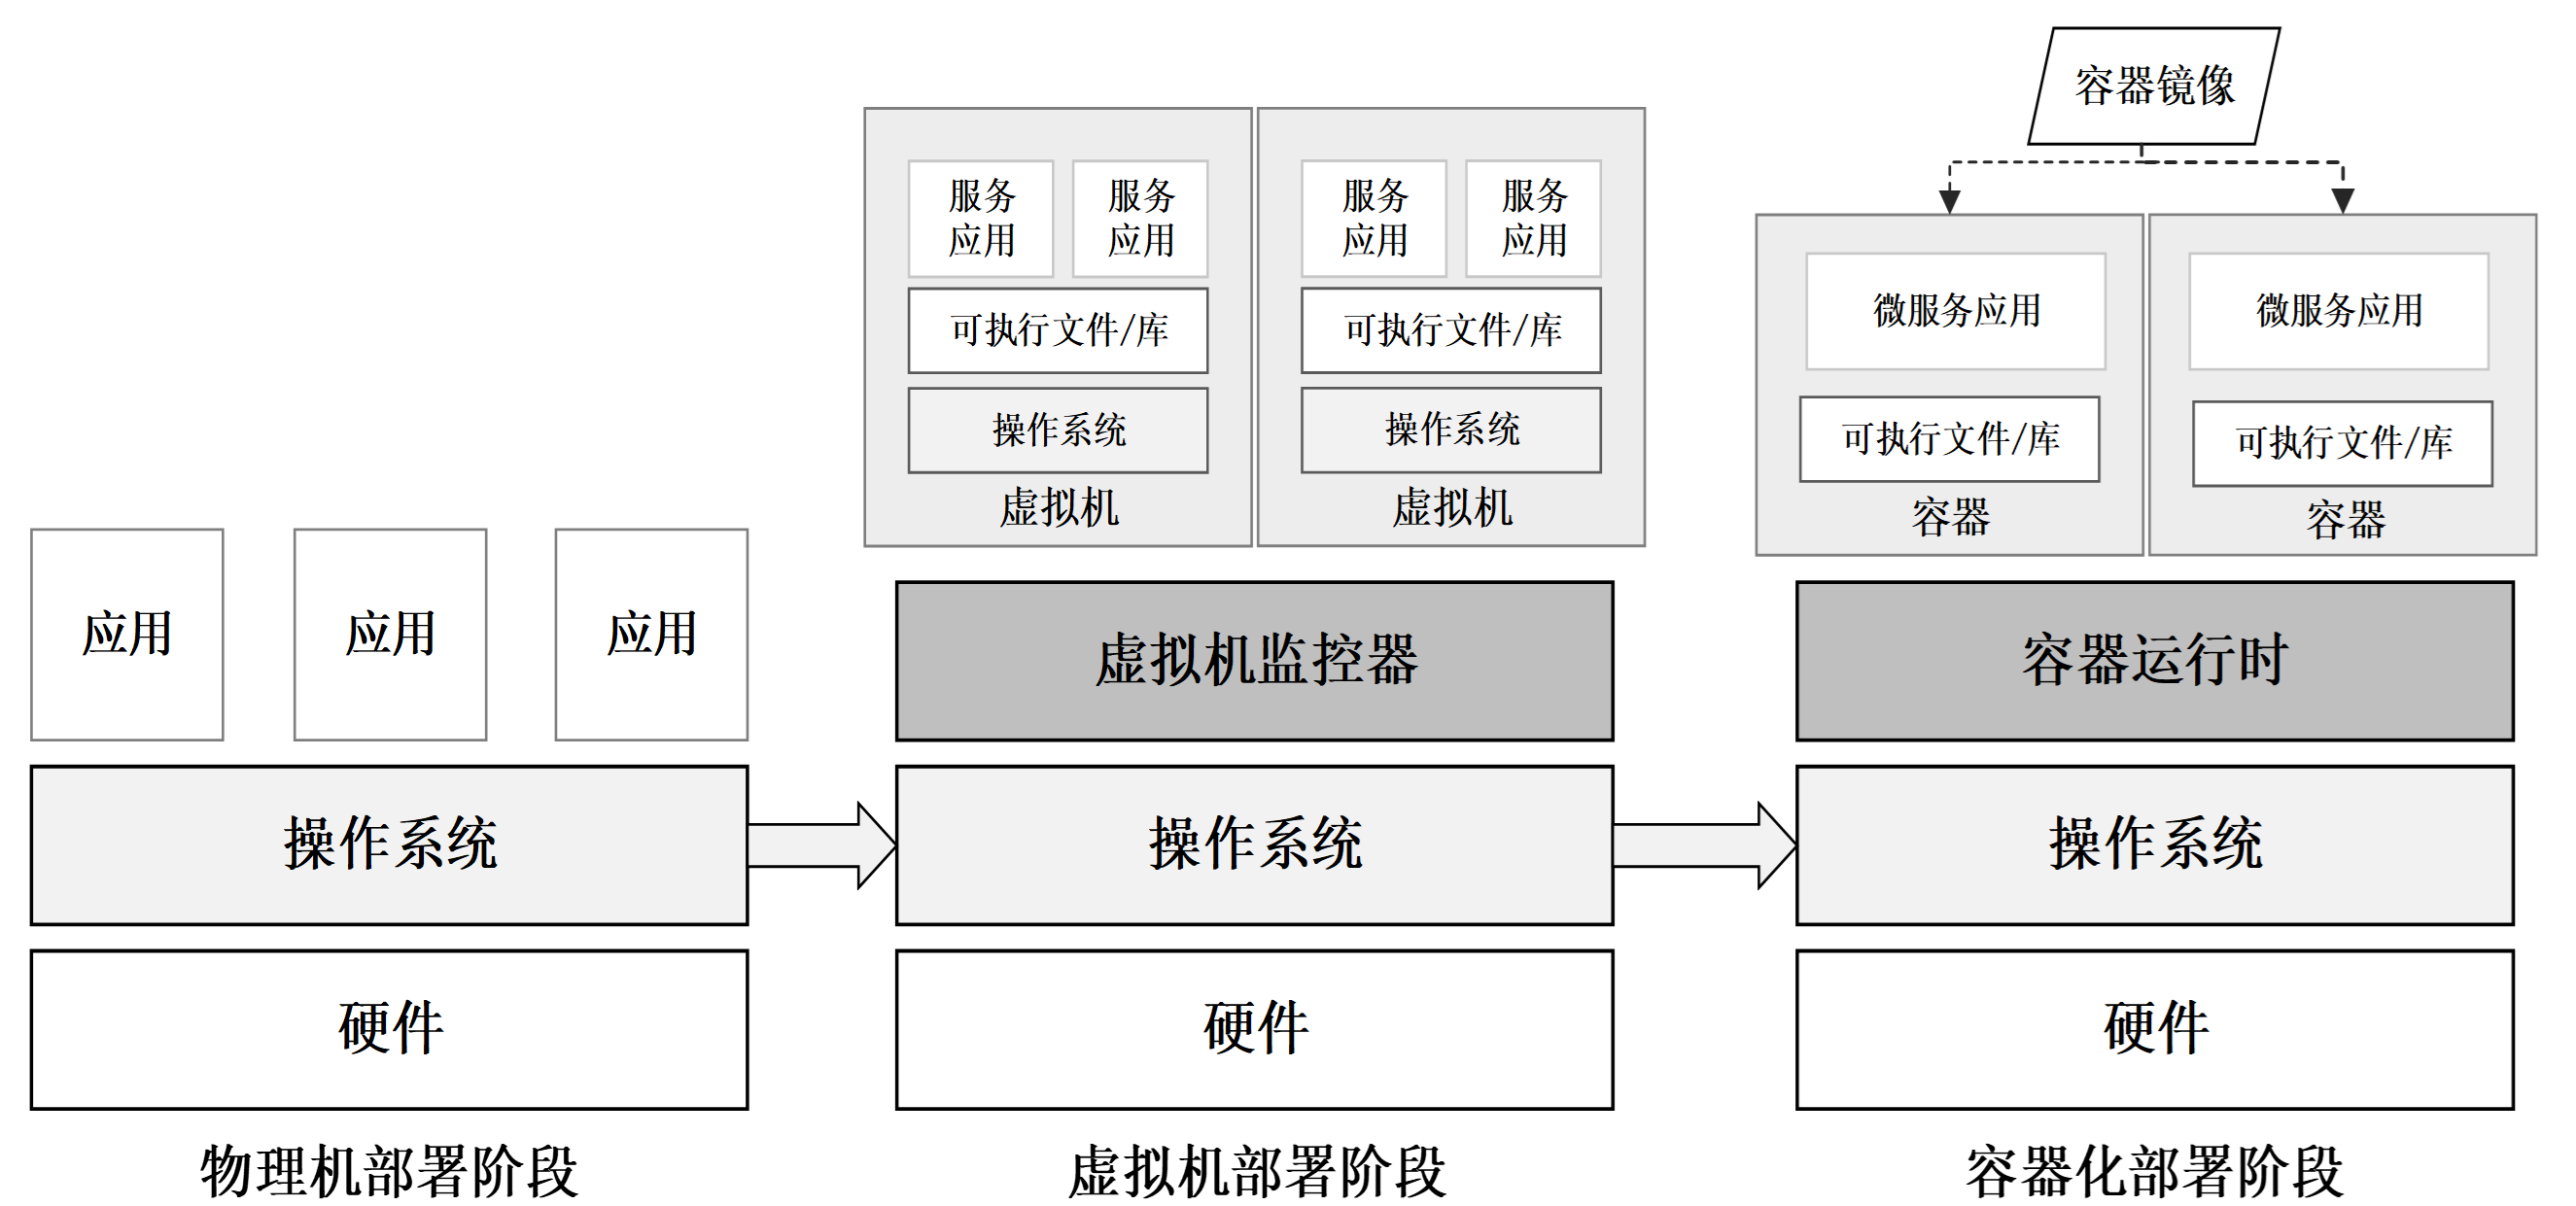
\includegraphics[width=0.9\linewidth]{images/容器.png}
    \bicaption{服务部署形式演进}{Evolution of service deployment paradigms}\label{fig:container-evolution}
\end{figure}

\begin{itemize}
    \item \textbf{命名空间（Namespace）隔离}：通过隔离进程、网络、挂载点等，使容器内运行的程序有独立系统抽象资源；
    \item \textbf{控制组（Cgroup）限制}：负责对容器施加 CPU、内存等硬件资源使用的强制规划，提供物理资源隔离；
    \item \textbf{只读分层与隔离挂载}：利用 OverlayFS 等联合文件系统\cite{wright2006versatility}，通过复用底层只读镜像并叠加独立的顶层读写区域，实现容器文件系统隔离。
\end{itemize}


\subsection{容器集群系统Kubernetes}
Kubernetes 是面向容器群集负载的分布式编排系统，简称K8S。源自于谷歌内部的虚拟化编排系统Borg\cite{Verma_2015}并在2014年正式对外开源。其核心思想是以\textbf{声明式 API}描述期望状态，再由控制平面持续驱动集群内容器向期望状态收敛\cite{kubernetes2024}。
\begin{figure}[htb]
    \centering
    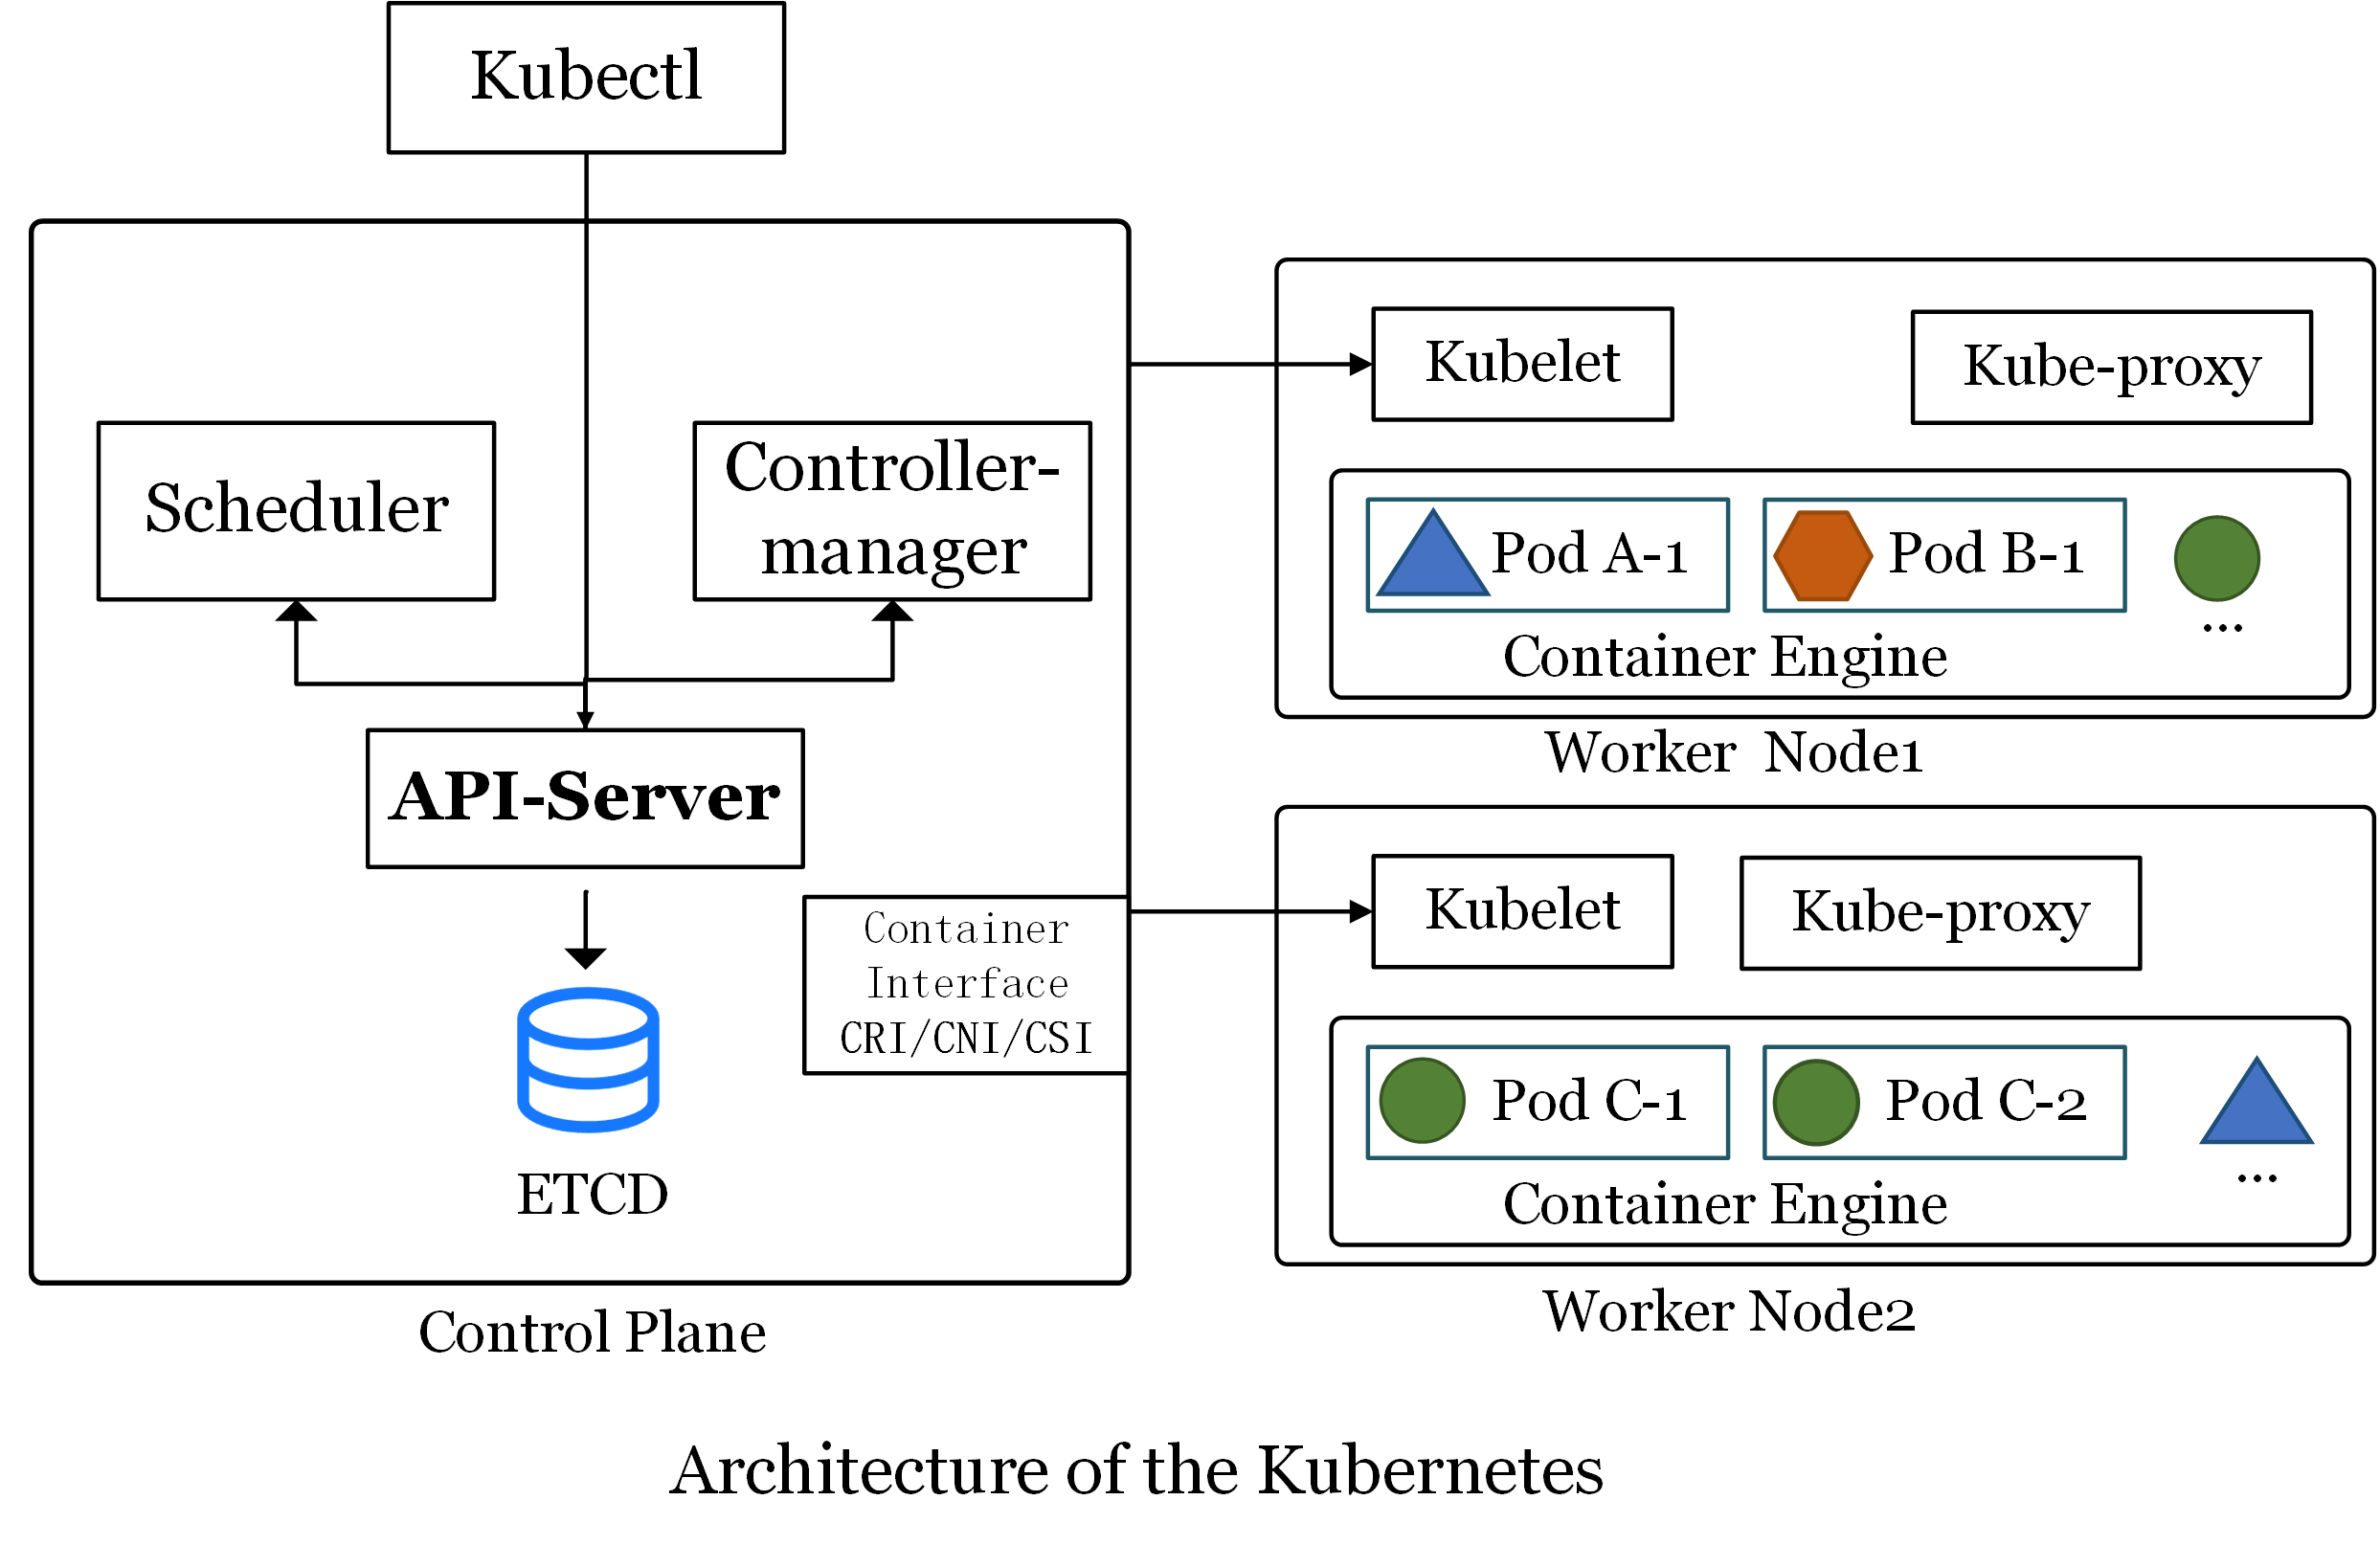
\includegraphics[width=0.8\textwidth]{images/k8s.png}
    \bicaption{Kubernetes 体系结构示意}{Overview of Kubernetes architecture}\label{fig:k8s-arch}
\end{figure}
图\ref{fig:k8s-arch}为 Kubernetes 的体系结构示意图，一个 Kubernetes 集群由\textbf{控制平面}与多个\textbf{工作节点}构成。控制平面负责提供控制接口、调度与集群控制逻辑，其中：\textbf{API Server}是所有资源访问与状态变更的统一入口，基于键值数据库ETCD承担认证、授权、准入与资源对象持久化等关键职责；\textbf{调度器}根据资源请求、亲和/反亲和等约束为工作负载选择节点；\textbf{控制器}负责提供控制与调节不同资源。工作节点侧，\textbf{kubelet}负责与API Server通信并维护调度到本节点的容器运行，\textbf{容器运行时}负责拉取镜像、创建容器并管理生命周期，\textbf{kube-proxy}负责服务转发与网络规则的实现。

Kubernetes通过一系列持久化\textbf{资源对象}表示集群对多种资源的编排与管理。例如，\textbf{Pod}是最小调度单元，包含一个或多个共享网络与存储的容器；Deployment/StatefulSet/DaemonSet分别面向无状态、有状态与节点守护型工作负载提供期望副本与更新策略；Service与Endpoint/EndpointSlice提供稳定的服务发现与负载均衡抽象；Ingress面向南北向流量提供入口控制；ConfigMap/Secret用于配置与敏感信息的声明式注入；Volume/PV/PVC则提供存储生命周期与绑定关系的抽象。


\subsection{Kubernetes 权限模型}
基于角色的访问控制（$\mathrm{RBAC}$）是 $\mathrm{Kubernetes}$ 授权机制的核心\cite{kubernetes2024}。图~\ref{fig:k8s-rbac-yaml}左侧展示了权限元模型的形式化表达，该权限模型可概括为\textbf{主语、动作与对象}的对应关系，即界定何种实体被允许对何种目标资源执行特定操作，其中：
\begin{itemize}
    \item \textbf{服务账户（ServiceAccount）}对应模型中的主语节点，代表发起请求的身份载体。在Kubernetes工作负载中每个Pod都有自己的服务账户。
    \item \textbf{权限角色（Role/ClusterRole）}对应模型中的动作与对象约束。该组件声明了在特定作用域内，针对各类资源（$\mathrm{resources}$）所允许执行的操作动词（$\mathrm{verbs}$）集合。
    \item \textbf{角色绑定（RoleBinding/ClusterRoleBinding）}作为关联映射机制，将服务账户与权限角色绑定以完成授权。
\end{itemize}

图~\ref{fig:k8s-rbac-yaml} 右侧展示了一个典型的 $\mathrm{RBAC}$ 授权流程示例：首先创建一个名为 $\mathrm{kada}$ 的 $\mathrm{ServiceAccount}$；随后定义名为 \texttt{basic-operation} 的 $\mathrm{Role}$，在其 $\mathrm{rules}$ 字段中授予对 $\mathrm{pods}$ 与 $\mathrm{secrets}$ 的 $\mathrm{get}$、$\mathrm{list}$、$\mathrm{create}$ 权限；最后通过 $\mathrm{RoleBinding}$ 将该 $\mathrm{Role}$ 绑定至 $\mathrm{kada}$ 账户。这种配置在接入第三方应用时很常见，但如果防范不当配置了过大的权限，将引发权限提升漏洞的风险。
\begin{figure}[htb]
    \centering
    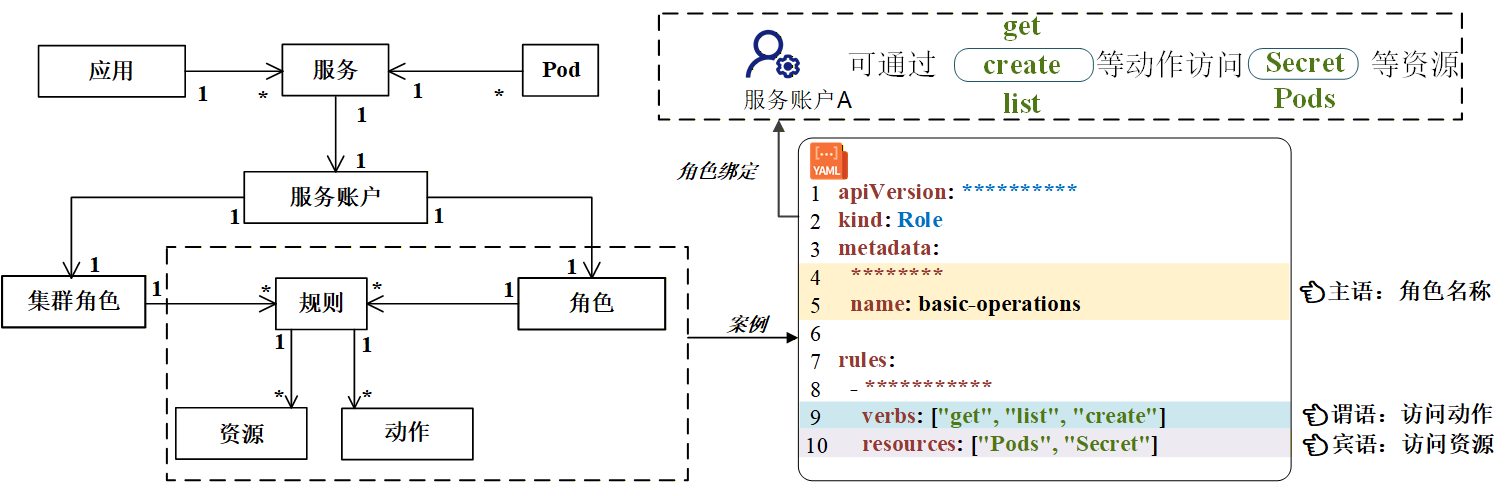
\includegraphics[width=0.95\textwidth]{images/yaml.png}
    \bicaption{Kubernetes RBAC 权限配置YAML文件示意\cite{kubeguard_icws2025}}{Example of Kubernetes RBAC permission configuration in YAML\cite{kubeguard_icws2025}}\label{fig:k8s-rbac-yaml}
\end{figure}

\subsection{Kubernetes 权限提升漏洞}

权限提升指攻击者在仅具备受限权限或初始执行能力的情况下，借助漏洞或错误配置，将自身权限提升到更高等级的过程\cite{mead2003computer}。在 Kubernetes 场景下，权限提升既可能表现为授权范围的扩大或横向获取，也可能表现为节点侧系统权限提升，从而对更大范围的资源与工作负载产生影响。

在云原生环境中，权限提升的危害往往具有更强的放大效应。一方面，单个节点通常承载多个 Pod，节点侧权限提升成功后，攻击者可能对同节点上的多个工作负载实施窃取敏感信息、篡改运行环境或注入恶意组件等行为。另一方面，Kubernetes 的资源对象与运维动作高度集中且自动化，控制平面授权不当同样会放大攻击后果。结合图~\ref{fig:k8s-rbac-yaml}中的示例，若主体被授予针对 $\texttt{Secret}$ 的 $\mathrm{get}/\mathrm{list}$ 权限，攻击者即可读取服务账户令牌、数据库口令或 API 密钥等敏感信息；若被授予针对 $\texttt{Pod}$ 的 $\mathrm{create}$ 权限，则可能进一步创建携带恶意镜像、特权配置或宿主机挂载的工作负载，作为横向移动、凭据窃取乃至后续节点侧利用的跳板。

图\ref{fig:cve-2024-33522} 以 \texttt{CVE-2024-33522} 为例展示了典型的节点侧权限提升漏洞。该漏洞源于 Calico CNI 安装程序的 SUID 位配置不当。若攻击者借助弱口令或服务暴露等前置手段获取了节点的本地访问权限，便可注入恶意二进制文件，并诱导安装程序以高权限执行。越权成功后，攻击者能直接接管容器运行时数据、窃取各类高优凭据并干扰网络组件，其危害将突破单一工作负载的隔离边界，迅速蔓延至整个集群。

\begin{figure}[htb]
    \centering
    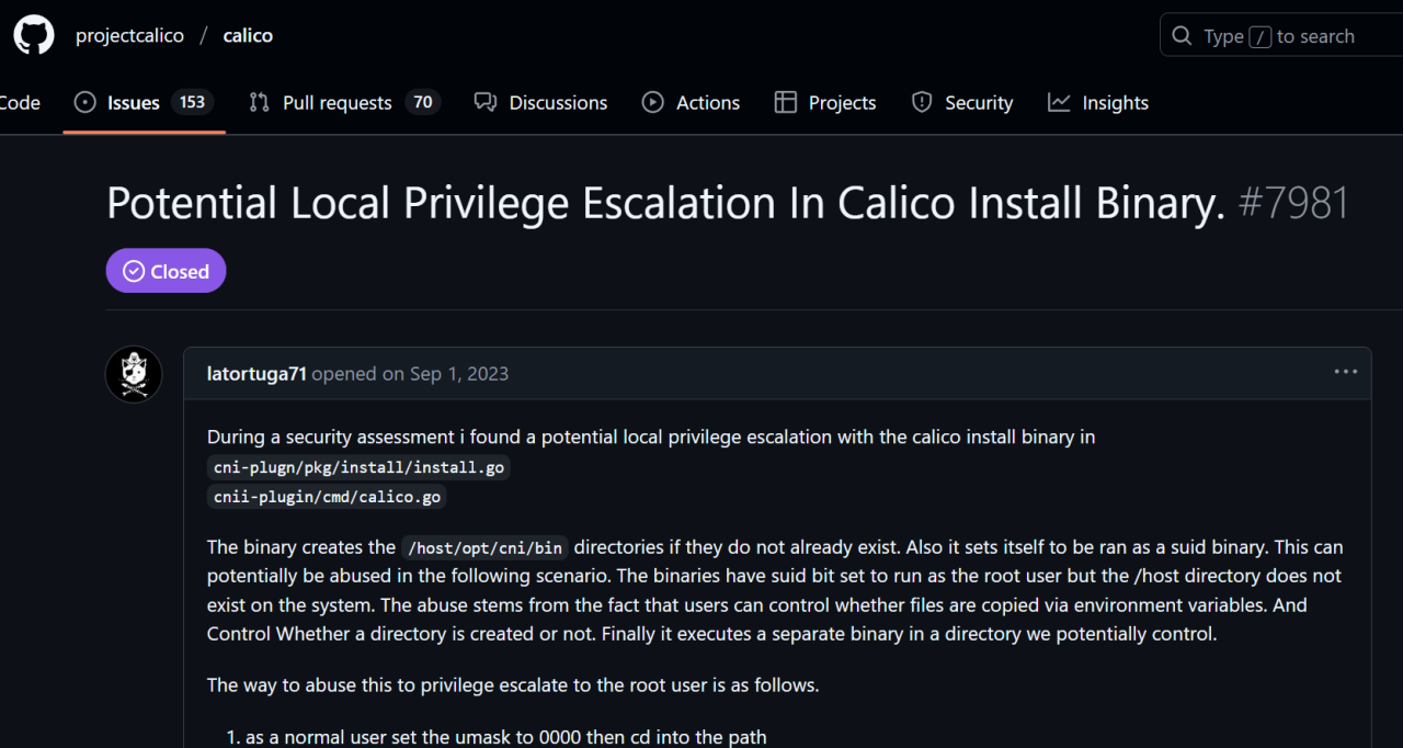
\includegraphics[width=1\textwidth]{images/cve_example.png}
    \bicaption{\texttt{CVE-\allowbreak2024-\allowbreak33522}（Calico）节点侧权限提升漏洞报告ISSUE}{Issue report of node-side privilege escalation vulnerability \texttt{CVE-\allowbreak2024-\allowbreak33522} in Calico}\label{fig:cve-2024-33522}
\end{figure}


\section{云原生安全工具}

云原生安全工具为 Kubernetes 集群提供全生命周期的安全风险监管机制。相关安全工具可基于规则化DSL代码对容器镜像、静态配置、集群系统行为、容器运行时等维度进行安全检查。下文将介绍几种广泛使用的云原生安全工具。

\subsection{监控工具：Falco}
Falco\cite{falco2025} 是云原生环境下广泛使用的开源容器运行时威胁检测引擎，其主要作用是为集群工作负载提供实时的异常行为监控与告警能力。在实现原理上，Falco 的机制包含内核态数据采集与规则引擎分析两个核心维度：它利用 eBPF 技术\cite{hoiland2018express}在内核层以极低侵入性的方式动态捕获各类系统调用事件，并将其转换为富含云原生上下文的事件流，随后交由基于领域特定语言构建的声明式规则引擎进行模式匹配，从而在不阻断正常业务的前提下识别并捕获风险行为。Falco同时也支持K8s业务监控，如K8s事件、K8s资源对象、K8s API调用等。

例如图\ref{fig:falco}展示了用于监测容器内启动交互式 shell 进程的规则。这种白盒化的检测方式具备极强的可解释性，能将告警直接关联至云原生实体，缩短安全定位路径。但该机制也存在一定的局限性：一方面，静态规则高度依赖专家知识的持续更新，对未知与变种攻击的泛化能力较弱；另一方面，其观测视野主要局限于系统调用层，难以有效感知应用层协议滥用或纯内存型的攻击。
\begin{figure}[htb]
    \centering
    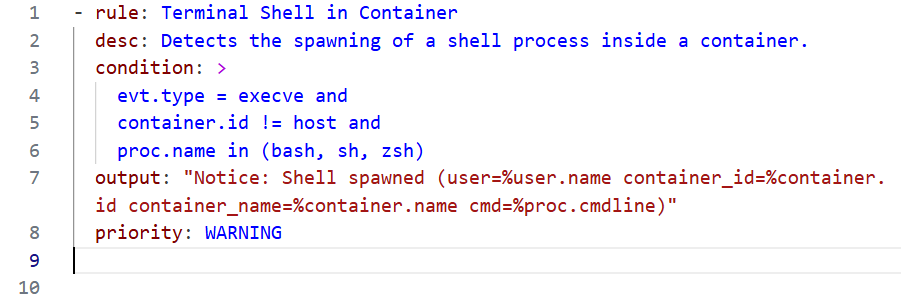
\includegraphics[width=0.8\textwidth]{images/falco.png}
    \bicaption{Falco 运行时监控与规则示意}{Illustration of Falco runtime monitoring and rules}\label{fig:falco}
\end{figure}

\subsection{防护工具：准入控制工具}
准入控制是 Kubernetes 中典型的事前防护机制。在 API Server 将资源持久化之前执行规则化校验，拦截特权容器、危险挂载、敏感权限增加等高风险配置变更。主流方案中，OPA/Gatekeeper 依托 Rego 语言，适合表达复杂组织策略；Kyverno 则采用 YAML 描述规则，更贴近运维习惯，落地成本更低。在补丁窗口期，这种规则化准入控制能够快速阻拦漏洞相关敏感资源操作。如图~\ref{fig:kyverno-demo} 所示，该Kyverno策略可以拒绝未携带 owner 标签的 Pod 创建请求。
\begin{figure}[htb]
    \centering
    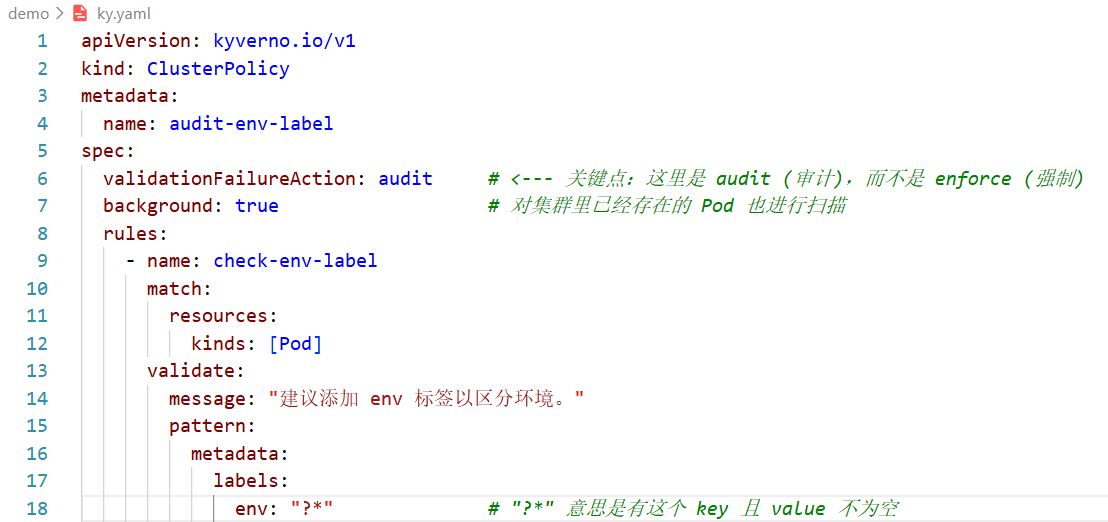
\includegraphics[width=0.8\linewidth]{images/kyverno.png}
    \bicaption{Kyverno 策略示例：强制要求 Pod 包含 owner 标签}{Example of a Kyverno policy enforcing owner labels on Pods}\label{fig:kyverno-demo}
\end{figure}

\subsection{网络防护工具：NetworkPolicy}
网络隔离用于降低横向移动与数据外传风险，是云原生环境中与身份权限控制互补的关键手段。Kubernetes 的 NetworkPolicy 为声明式防护策略，在多租户或微服务体系中可将控制域落到命名空间与工作负载级别，减少单点被攻破后对整个集群的扩散影响。常见的Kubernetes网络插件（如 Calico、Cilium、Weave Net 等）均支持 NetworkPolicy 的实现。
\begin{figure}[htb]
    \centering
    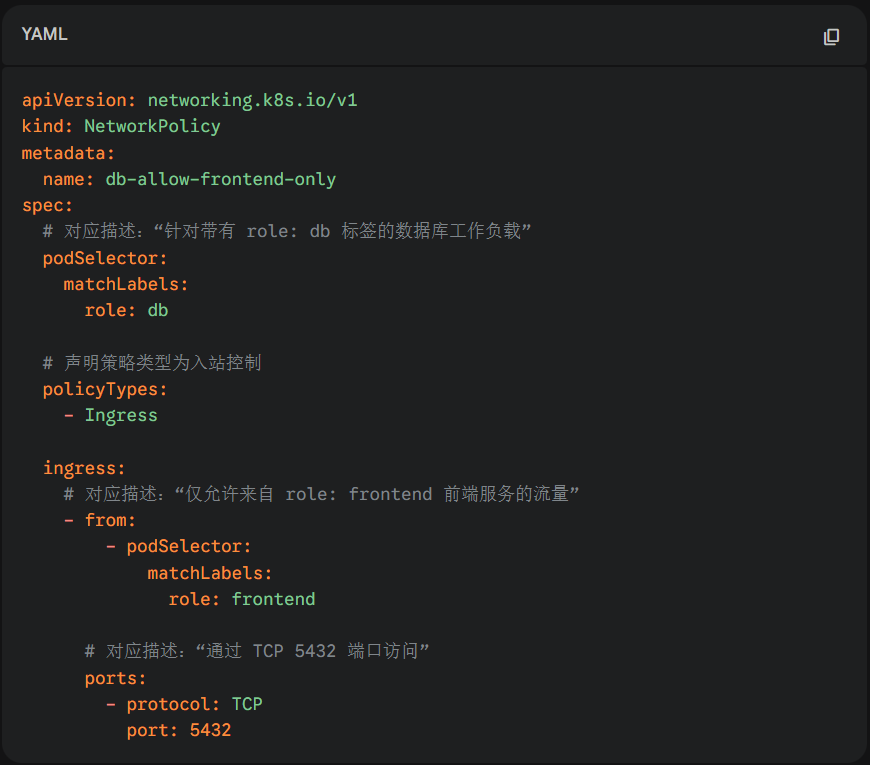
\includegraphics[width=0.8\linewidth]{images/networkpolicy.png}
    \bicaption{NetworkPolicy 示例：限制数据库仅允许前端服务访问}{Example of a NetworkPolicy allowing only frontend services to access the database}\label{fig:networkpolicy-demo}
\end{figure}

如图~\ref{fig:networkpolicy-demo} 所示，该策略定义了一个典型的微服务网络隔离场景：针对带有 \texttt{role: db} 标签的数据库工作负载，仅允许来自 \texttt{role: frontend} 前端服务的流量通过 TCP 5432 端口访问。这种基于标签选择器（Label Selector）的白名单机制有效地构建了微服务隔离边界，确保即使集群内其他容器试图横向移动访问数据库，也会在网络层被直接阻断。

\subsection{静态扫描与配置审计工具}
与运行时检测相对，静态扫描更偏向事前发现与持续治理。静态扫描在镜像构建、交付与部署前，通过自动化检查提前识别已知漏洞、弱配置与合规风险，避免高风险对象进入集群。

第一类是\textbf{镜像与依赖漏洞扫描}。该类工具通常解析镜像分层文件系统与软件包清单，基于公开漏洞库对已知 CVE 进行匹配，并输出风险等级、受影响版本与修复建议。代表性工具包括 Trivy\cite{trivy2025}、Grype/Anchore\cite{grype2025} 等；其中，Syft\cite{syft2025} 等工具可生成软件物料清单（SBOM），用于提升漏洞告警的可追溯性与供应链治理能力。

第二类是\textbf{Kubernetes 清单与基础设施即代码（IaC）扫描}。这类工具面向 YAML、Helm、Terraform 等配置，以规则化方式识别特权容器、宿主机路径挂载、过宽权限、明文密钥及资源限制缺失等风险，可用于代码评审、部署前基线核查与准入前置门禁。典型工具包括面向工作负载清单的 kube-linter\cite{kubelinter2025}、Kubescape\cite{kubescape2025}、kube-score\cite{kubescore2025}、KubeSec\cite{kubesec2025}、Polaris\cite{polaris2025}，以及面向 IaC 模板的 Checkov\cite{checkov2025}；针对权限审计的工具包括 KubiScan\cite{kubiscan2024}、Krane\cite{krane2024}、RBAC Police\cite{paloalto2024}。此类方法易于规模化落地，但也可能因业务差异产生误报，因此需要进行人工二次审查。表\ref{tab:k8s-security-scan-tools}对 Kubernetes 常见安全扫描与审计工具进行分类整理。
\begin{table}[htb!]
    \centering\bicaption{Kubernetes 常见安全扫描与审计工具整理}{Classification of common Kubernetes security scanning and auditing tools}\label{tab:k8s-security-scan-tools}
    \noindent\renewcommand{\arraystretch}{1.25}
    \setlength{\tabcolsep}{1.5mm}
    \small
    \begin{tabular}{>{\centering\arraybackslash}m{2.2cm}m{5.5cm}>{\raggedright\arraybackslash}m{4.0cm}}
    \toprule
    \textbf{类别} & \textbf{代表性工具} & \textbf{主要用途}\\
    \midrule
    镜像/依赖漏洞扫描
    & \texttt{Trivy}、\texttt{Grype}、\texttt{Clair}、\texttt{Snyk}
    & 发现镜像与依赖漏洞，用于 CI 门禁、制品准入与修复建议。\\
    \midrule
    SBOM 生成与供应链
    & \texttt{Syft}、\texttt{CycloneDX}、\texttt{cosign}
    & 生成 SBOM 与签名校验，用于供应链追溯和完整性校验。\\
    \midrule
    配置与 IaC 安全扫描
    & \texttt{Kubescape}、\texttt{kube-score}、\texttt{kube-linter}、\texttt{Polaris}、\texttt{KubeSec}、\texttt{datree}、\texttt{Checkov}、\texttt{KICS}、\texttt{tfsec}
    & 扫描 YAML/Helm/IaC 弱配置与基线违规，用于评审和部署前核查。\\
    \midrule
    RBAC/权限审计
    & \texttt{KubiScan}、\texttt{Krane}、\texttt{RBAC Police}、\texttt{kubeaudit}、\texttt{rakkess}、\texttt{kubectl-who-can}
    & 审计角色、绑定和账户权限，用于过宽授权识别与权限查询。\\
    \bottomrule
    \end{tabular}
\end{table}


\section{国内外研究现状}

本节按照通用系统权限安全研究、Kubernetes 场景安全研究和课题组已有工作这一顺序展开。前两部分分别概括权限提升风险在一般系统与云原生环境中的研究脉络，最后结合课题组前期成果说明本文工作的承接关系与问题切入点。

\subsection{系统权限安全问题}
系统权限安全研究最初聚焦访问控制模型与最小授权原则，随后逐步扩展到对过度授权、运行时提权行为和信息流泄露的综合治理。在基础设计原则层面，Saltzer 与 Schroeder\cite{saltzer1975protection}于 1975 年指出，\textbf{最小权限原则}是实现特权隔离的重要基础。基于这一原则，Ferraiolo 等\cite{ferraiolo1995role}提出基于角色的访问控制模型（RBAC），以角色组织多类权限并将其映射至不同主体，缓解了规模化授权中的管理难题。然而，\textbf{过度授权}现象普遍存在，显著扩大了系统攻击面\cite{o1995redundant}。为收敛这类风险，Molloy 等\cite{molloy2012generative}以及 Sanders 与 Yue\cite{sanders2018minimizing}分别提出基于日志与算法模型逆向生成应用最小权限集的策略，使权限治理由静态制度设计进一步走向结合实际使用行为的最小权限推断。

随着系统组件化程度不断提高，权限提升风险不再局限于单一主体的越权访问，而更多表现为跨组件、跨应用甚至跨平台的调用链滥用。在典型移动操作系统 Android 中，访问控制的粗粒度特性带来了更为突出的权限提升与隐蔽滥用风险。Davi 等人\cite{davi2010privilege}较早揭示了\textbf{混淆代理}攻击模型，即低权限应用可通过伪造合法请求，诱导高权限组件执行敏感操作。Hutchinson 等\cite{hutchinson2018survey}进一步将该模型概括为三个条件：请求敏感权限、开放导出组件以及存在通向敏感 API 的执行路径。随着攻防对抗持续升级，提权漏洞的利用方式也由单一组件劫持\cite{wu2016seccomp}，演变为多重调用链上的跨应用共谋\cite{elzawawy2025hidden}，甚至扩展至同一设备内由第三方 SDK 发起的共谋攻击\cite{taylor2017intralibrary}。

围绕上述风险，现有治理方法大致可归纳为静态架构分析、动态行为监控和数据流追踪三类。静态方法中，Au 等\cite{au2012pscout}提出 PScout，通过分析系统源码自动提取底层权限检查图谱；后续研究进一步结合最小执行权限要求引入强制访问控制机制：Bagheri 等\cite{bagheri2019deldroid}提出 DelDroid，通过静态分析自动推导并强制实施应用所需的最小权限架构；Wu 等\cite{wu2016seccomp}提出 SecComp，在组件调用层面约束非授权操作以防御劫持攻击。动态方法中，相关研究结合进程代数建模\cite{xu2019adaptive}、系统级探针监控\cite{hussain2020framework}以及深度学习与半监督学习\cite{sharmeen2020adaptive}，实现运行期权限提升行为的拦截与预警。当授权边界被突破后，还可借助数据流监控开展后果溯源，相关研究已从面向 Web 的混合污点分析\cite{tripp2009taj}，拓展至 Android 系统层实时信息流监控（TaintDroid\cite{enck2014taintdroid}）和免 Root 的动态污点分析（TaintMan\cite{you2017taintman}）。整体来看，这一路径表明权限安全分析正由权限静态归属分析进一步转向对真实调用链利用过程的分析。

上述思路随后被扩展到小程序等宿主内嵌生态的权限安全研究。Zhang 等\cite{zhang2023small}对多个主流小程序生态开展系统性研究，提取了通用的权限控制抽象模型，揭示了跨运行态环境下的多类典型越权漏洞并通过实际攻击加以验证；Wang 等\cite{wang2024minichecker}则聚焦小程序数据权限滥用问题，定义了多种违规权限申请模式，并设计静态分析工具 MiniChecker 开展规模化检测，指出现有平台权限机制在底层设计上仍存在固有缺陷。总体来看，通用系统中的相关研究为识别跨组件调用、越权传播和后果溯源提供了重要方法基础，但其分析对象和执行环境与 Kubernetes 仍存在明显差异。

\subsection{Kubernetes 安全问题}
在云原生场景中，Kubernetes 将配置、控制平面、网络与运行时机制耦合在同一系统之中，权限风险往往沿部署模板、授权链路和组件交互同时扩散。因此，相关研究既继承了通用系统中的最小授权与行为检测思路，又形成了更强调配置语义和多层联动的分析路径。现有工作大体可分为配置风险识别、模板与 IaC 安全分析、架构与权限链风险挖掘以及网络与运行时防护四类。

安全误配置是 Kubernetes 场景中最常见、也最早受到关注的风险来源。早期研究主要用于勾勒配置风险的整体图景：Islam Shamim 等\cite{Islam_Shamim_2020}系统总结了 Kubernetes 安全实践，Shamim\cite{Shamim_2021}进一步指出部署清单偏离最佳实践可能直接演化为可利用的提权路径，Curtis 与 Eisty\cite{Curtis_2025}基于 Stack Overflow 数据的实证分析也表明配置安全始终是开发侧的核心关切。在此基础上，Rahman 等\cite{k8smanifests2023}对开源清单中的典型安全误配置进行了大规模归纳与实证研究。然而，仅依赖静态扫描难以完整反映风险的真实可利用性。Shamim 等\cite{shamim2025prescription}评估了 CIS 推荐配置的合规现状，发现从业人员对安全基线的理解存在显著差异，现有 SAST 工具的检测覆盖也有明显不足；其后续工作\cite{shamim2025dastk8s}进一步结合工业界部署实践，论证了将 DAST 动态分析纳入配置核验流程的客观必要性。上述研究说明，Kubernetes 配置安全研究正由基线合规判断转向实际可利用风险评估。

在识别单份清单风险之外，基础设施即代码（IaC）也被证明是 Kubernetes 安全风险的重要来源。针对 Helm Charts 带来的依赖传播与供应链风险，Zerouali 等\cite{Zerouali_2023}和 Blaise 与 Rebecchi\cite{Blaise_2022}分别从生态规模与依存关系角度提供了分析基础；Minna 等\cite{minna2025analyzing}进一步评估了大语言模型在修复 IaC 配置异味方面的效果与边界。为缓解多平台安全语义碎片化问题，Ul Haque 等\cite{KGSecConfig2022}提出知识图谱框架 KGSecConfig，对安全配置概念进行统一抽取与建模。这类研究表明，Kubernetes 安全治理已由局部规则检查逐步扩展到面向模板、依赖关系与安全语义的自动化分析。

仅分析配置项是否合规仍不足以解释攻击链如何形成，因此相关研究进一步深入到体系结构缺陷与过度授权所引发的链式风险。Dell'Immagine 等\cite{Dell_Immagine_2023}面向微服务部署定义了一组安全反模式，并实现自动检测工具 KubeHound，表明安全缺陷可能嵌入系统交互结构之中。Yang 等\cite{yang2023take}系统分析了 CNCF 生态中第三方插件的权限配置，设计了多种攻击路径利用策略，可将工作节点逃逸演化为全集群接管。Gu 等\cite{gu2024epscan}提出 EPScan，通过面向容器的程序分析自动比对实际资源访问行为与声明权限，识别可被利用的过度特权。与前述误配置研究相比，这一方向更关注风险沿授权链路的形成与放大机制。

即便控制平面配置与授权链路得到一定约束，底层网络与运行时隔离仍是 Kubernetes 安全防护不可缺少的一环。容器编排引入的网络抽象与传统安全模型存在显著差异，Minna 等\cite{Minna_2021}指出这种差异可能衍生非预期的攻击路径。在网络策略的工程落地层面，Budigiri 等\cite{Budigiri_2021}基于 eBPF 评估了网络策略的性能代价，Kim 等\cite{Kim_2025}对比了多种容器网络接口插件的安全能力，两项工作共同揭示了协议过滤深度与转发性能之间的固有权衡。在缓解机制方面，研究视角涵盖了从 DevOps 流水线到节点侧运行时的多个层面：Pecka 等\cite{pecka2022privilege}通过构造流水线攻击场景证明了工具合规并不等同于安全，Cesarano 与 Natella\cite{cesarano2025kubefence}提出的 KubeFence 通过裁剪非必要 API 参数实现了比 RBAC 更细粒度的接口过滤，Zhu 与 Gehrmann\cite{Zhu_2022}和 Le 等\cite{Le_2023}则分别在 AppArmor 配置自动生成与系统调用感知调度方向上强化了节点侧防护。综合来看，现有研究已经从清单级合规检查推进到跨组件授权链与运行时隔离的综合分析，但对于权限提升漏洞在暴露窗口期如何快速生成兼顾监控与防护的协同策略，仍缺乏统一方法框架。


\subsection{本课题组研究基础}
在上述研究基础上，课题组围绕 Kubernetes 权限风险检测开展了系统研究，已形成覆盖风险建模、原型实现与实验验证的前期积累。其中，代表性成果为 KubeGuard 框架。该框架面向过度权限、权限提升和敏感信息泄露三类风险，分别设计了最小权限集构建、规则化审计以及敏感词监测机制\cite{kubeguard_icws2025}。如图\ref{fig:kgf}所示，KubeGuard 由过度权限检测、权限提升检测和敏感信息泄露检测三个模块构成。

\begin{figure}[htb]
    \centering
    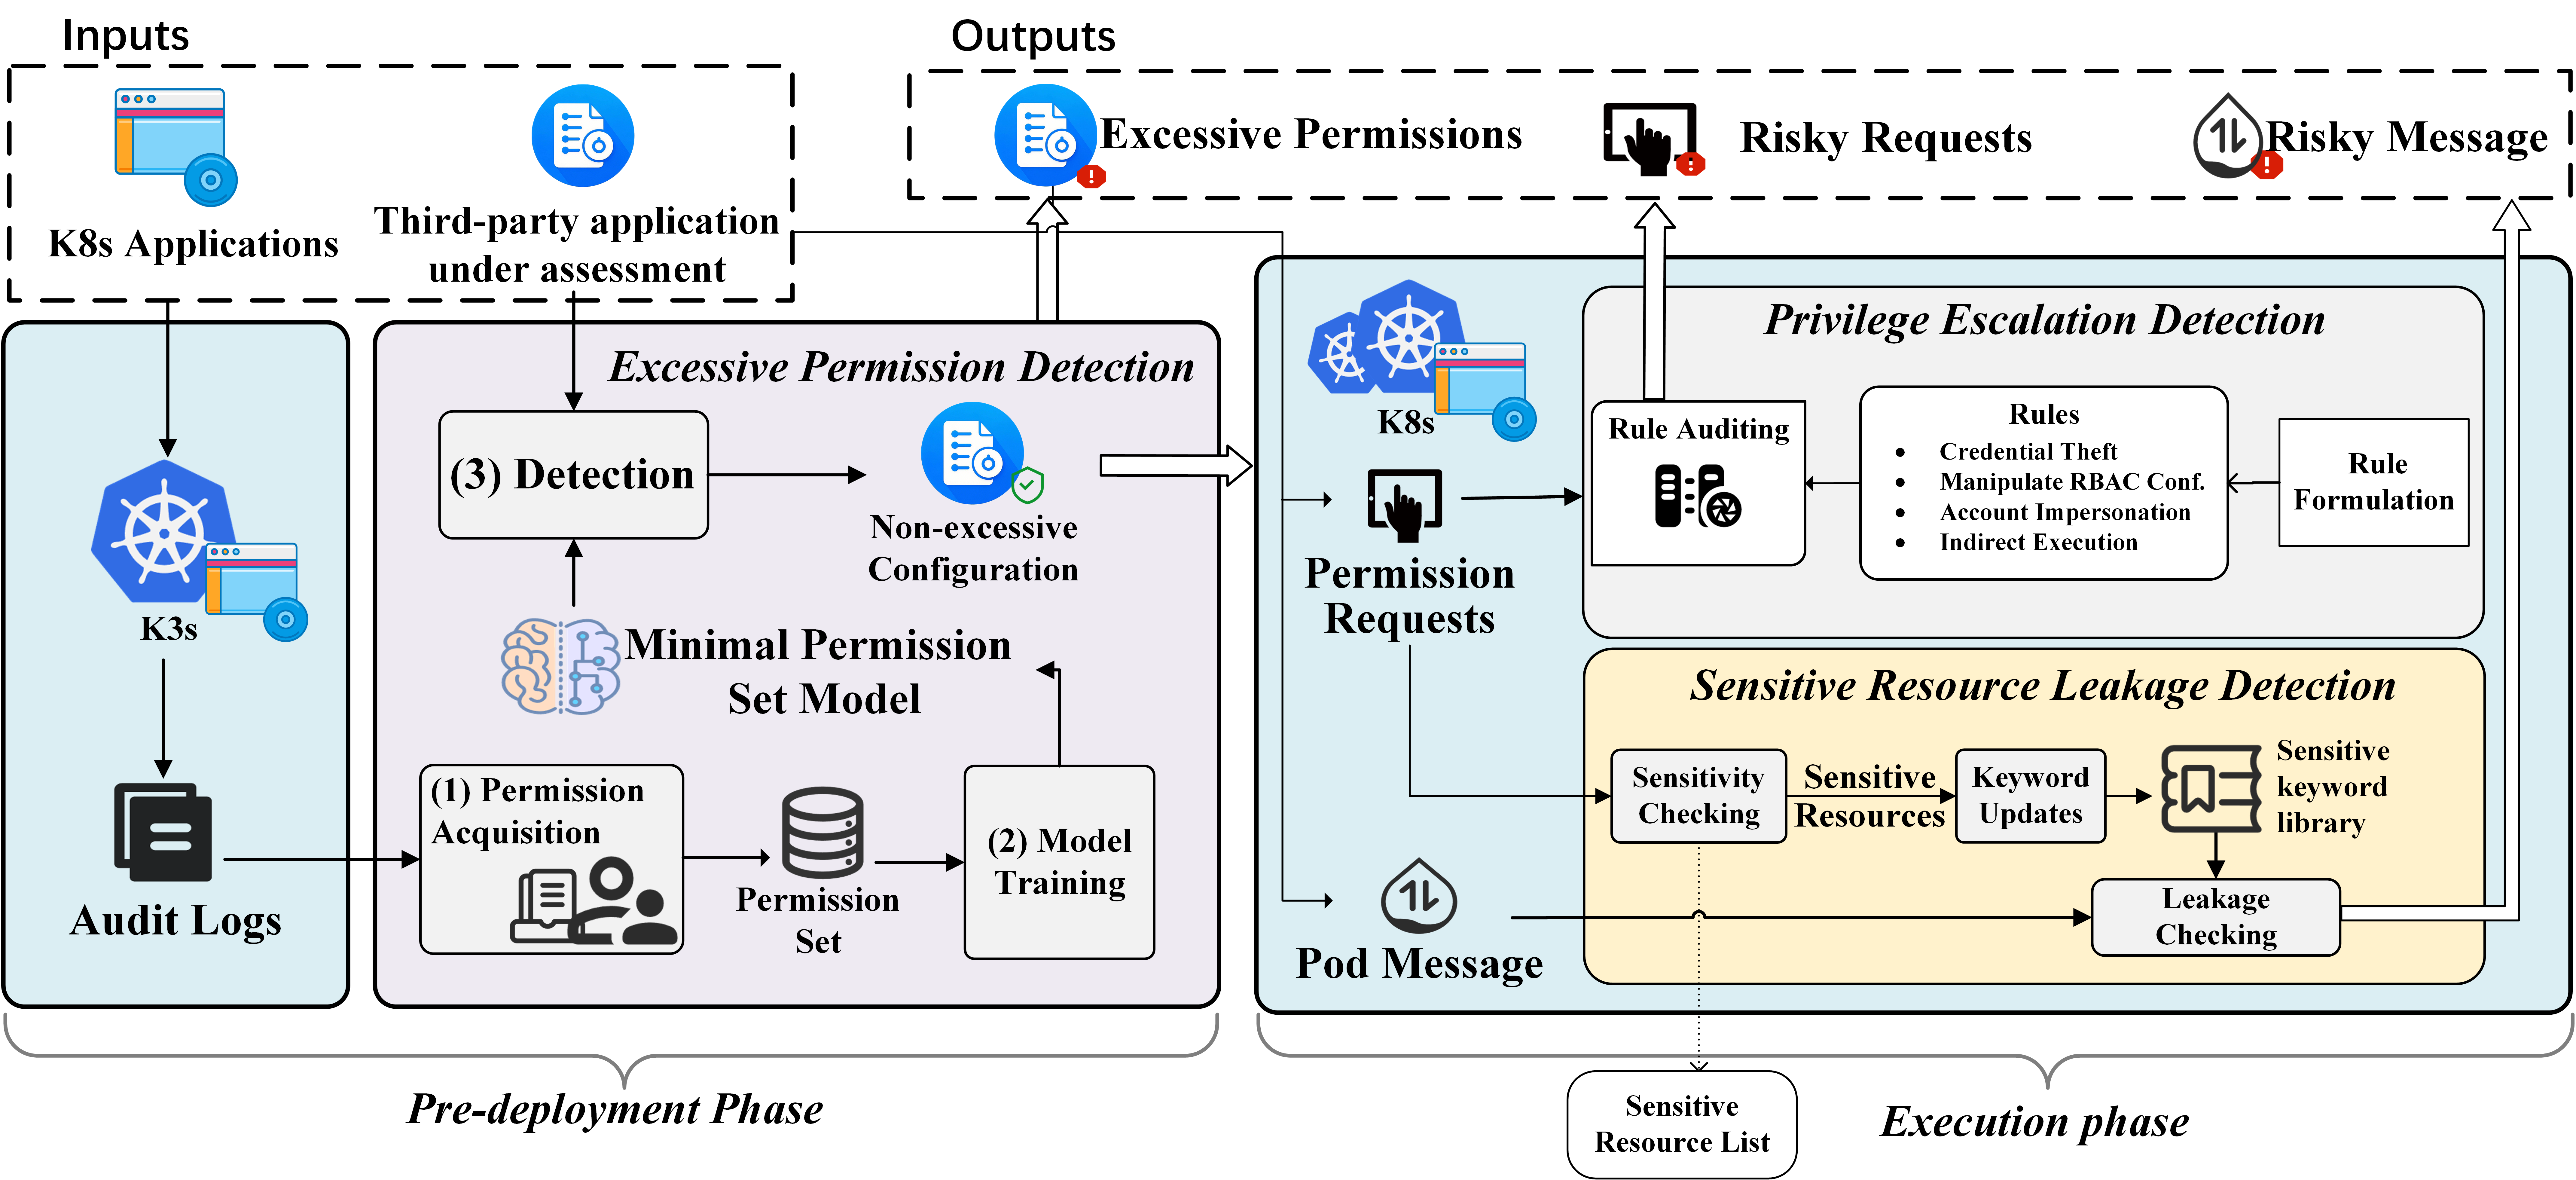
\includegraphics[width=0.95\textwidth]{images/KGF.png}
    \bicaption{KubeGuard 方法框架图\cite{kubeguard_icws2025}}{Framework of the KubeGuard method\cite{kubeguard_icws2025}}\label{fig:kgf}
\end{figure}

在方法设计上，KubeGuard 一方面利用 NLP 技术识别应用所需的最小权限集，以判定权限配置是否存在过度授权；另一方面通过动态规则审计检测多类权限提升风险。具体而言，该工作将权限提升场景归纳为凭证窃取、账户冒用、RBAC 操纵和间接执行四类，并针对各类场景提出相应的检测思路。考虑到规则细节较为繁杂，相关风险描述与检测规则在正文中不再展开，具体内容见附录表\ref{tab:PEDetectionRules}。此外，该框架还通过监测 Pod 间消息传输并结合关键词匹配，对涉及敏感资源的内容进行告警，从而覆盖敏感信息泄露风险。

在系统实现与效果验证方面，课题组进一步实现了原型系统 KubeGuarder，并在开源 Kubernetes 应用与模拟场景中开展实验评估\cite{kubeguard_icws2025}。实验结果表明，该系统在过度权限检测方面相较静态基线方法表现出更高的有效性与准确性，同时能够识别多类型的权限提升与敏感信息泄露风险。这说明前期工作已经验证了从权限视角开展风险建模与检测的可行性，并为本文进一步研究提供了方法与系统基础。

不过，现有工作仍主要停留在权限层面的规则化检测，其核心依据是 RBAC 配置与 API 访问行为之间的匹配关系。该方法虽然能够较为系统地覆盖多种权限提升模式，但在真实生产环境中仍存在三方面局限：（1）仅依据权限配置与操作行为的对应关系，难以准确区分正常运维行为与恶意提权行为，因此误报风险较高；（2）该方法主要面向控制平面与资源访问层，尚未深入节点侧系统层面的权限提升漏洞，对容器逃逸、SUID 配置不当及内核漏洞等底层利用缺乏针对性的检测能力；（3）基于预定义规则的检测方式对未知漏洞与新型攻击手法的泛化能力有限。上述不足也构成了本文进一步研究的直接出发点，即在保留权限视角优势的同时，引入面向真实利用链与运行态场景的检测与防护能力。


\section{小结}
本章介绍了容器、Kubernetes 及其权限模型等基础概念与云原生安全工具，并从系统权限安全、Kubernetes 安全与课题组前期工作三个层面梳理了国内外研究现状，为后续章节的方法设计与实验验证奠定了理论基础。


\chapter{面向云原生权限提升漏洞的智能化防控技术}\label{chap:method}


本章系统阐述面向云原生权限提升漏洞的智能化防控方法，先说明研究动机与方法框架，再介绍基本概念定义，并围绕知识库构建、多智能体策略生成与质量评估三项核心技术展开具体设计。

\section{研究动机}

本章讨论的问题，主要发生在漏洞已经披露但补丁尚未真正落地的处置阶段。对生产环境而言，第三方组件升级通常受到兼容性验证、变更审批与业务连续性要求等因素制约，补丁发布并不意味着系统能够立即完成修复。本文对 2020 至 2025 年间 55 个云原生权限提升漏洞的统计表明，$30.4\%$ 的漏洞因补丁延迟而长期处于可利用状态。与此同时，攻击者却可以借助公开公告、修复提交或社区讨论快速还原利用条件。因此，在补丁窗口期内形成临时防控措施，并尽快阻断关键利用条件、收敛攻击面和补足观测能力，已经成为云原生漏洞处置中的独立任务，而不只是正式修复前的附属动作。

\begin{figure}[htb]
    \centering
    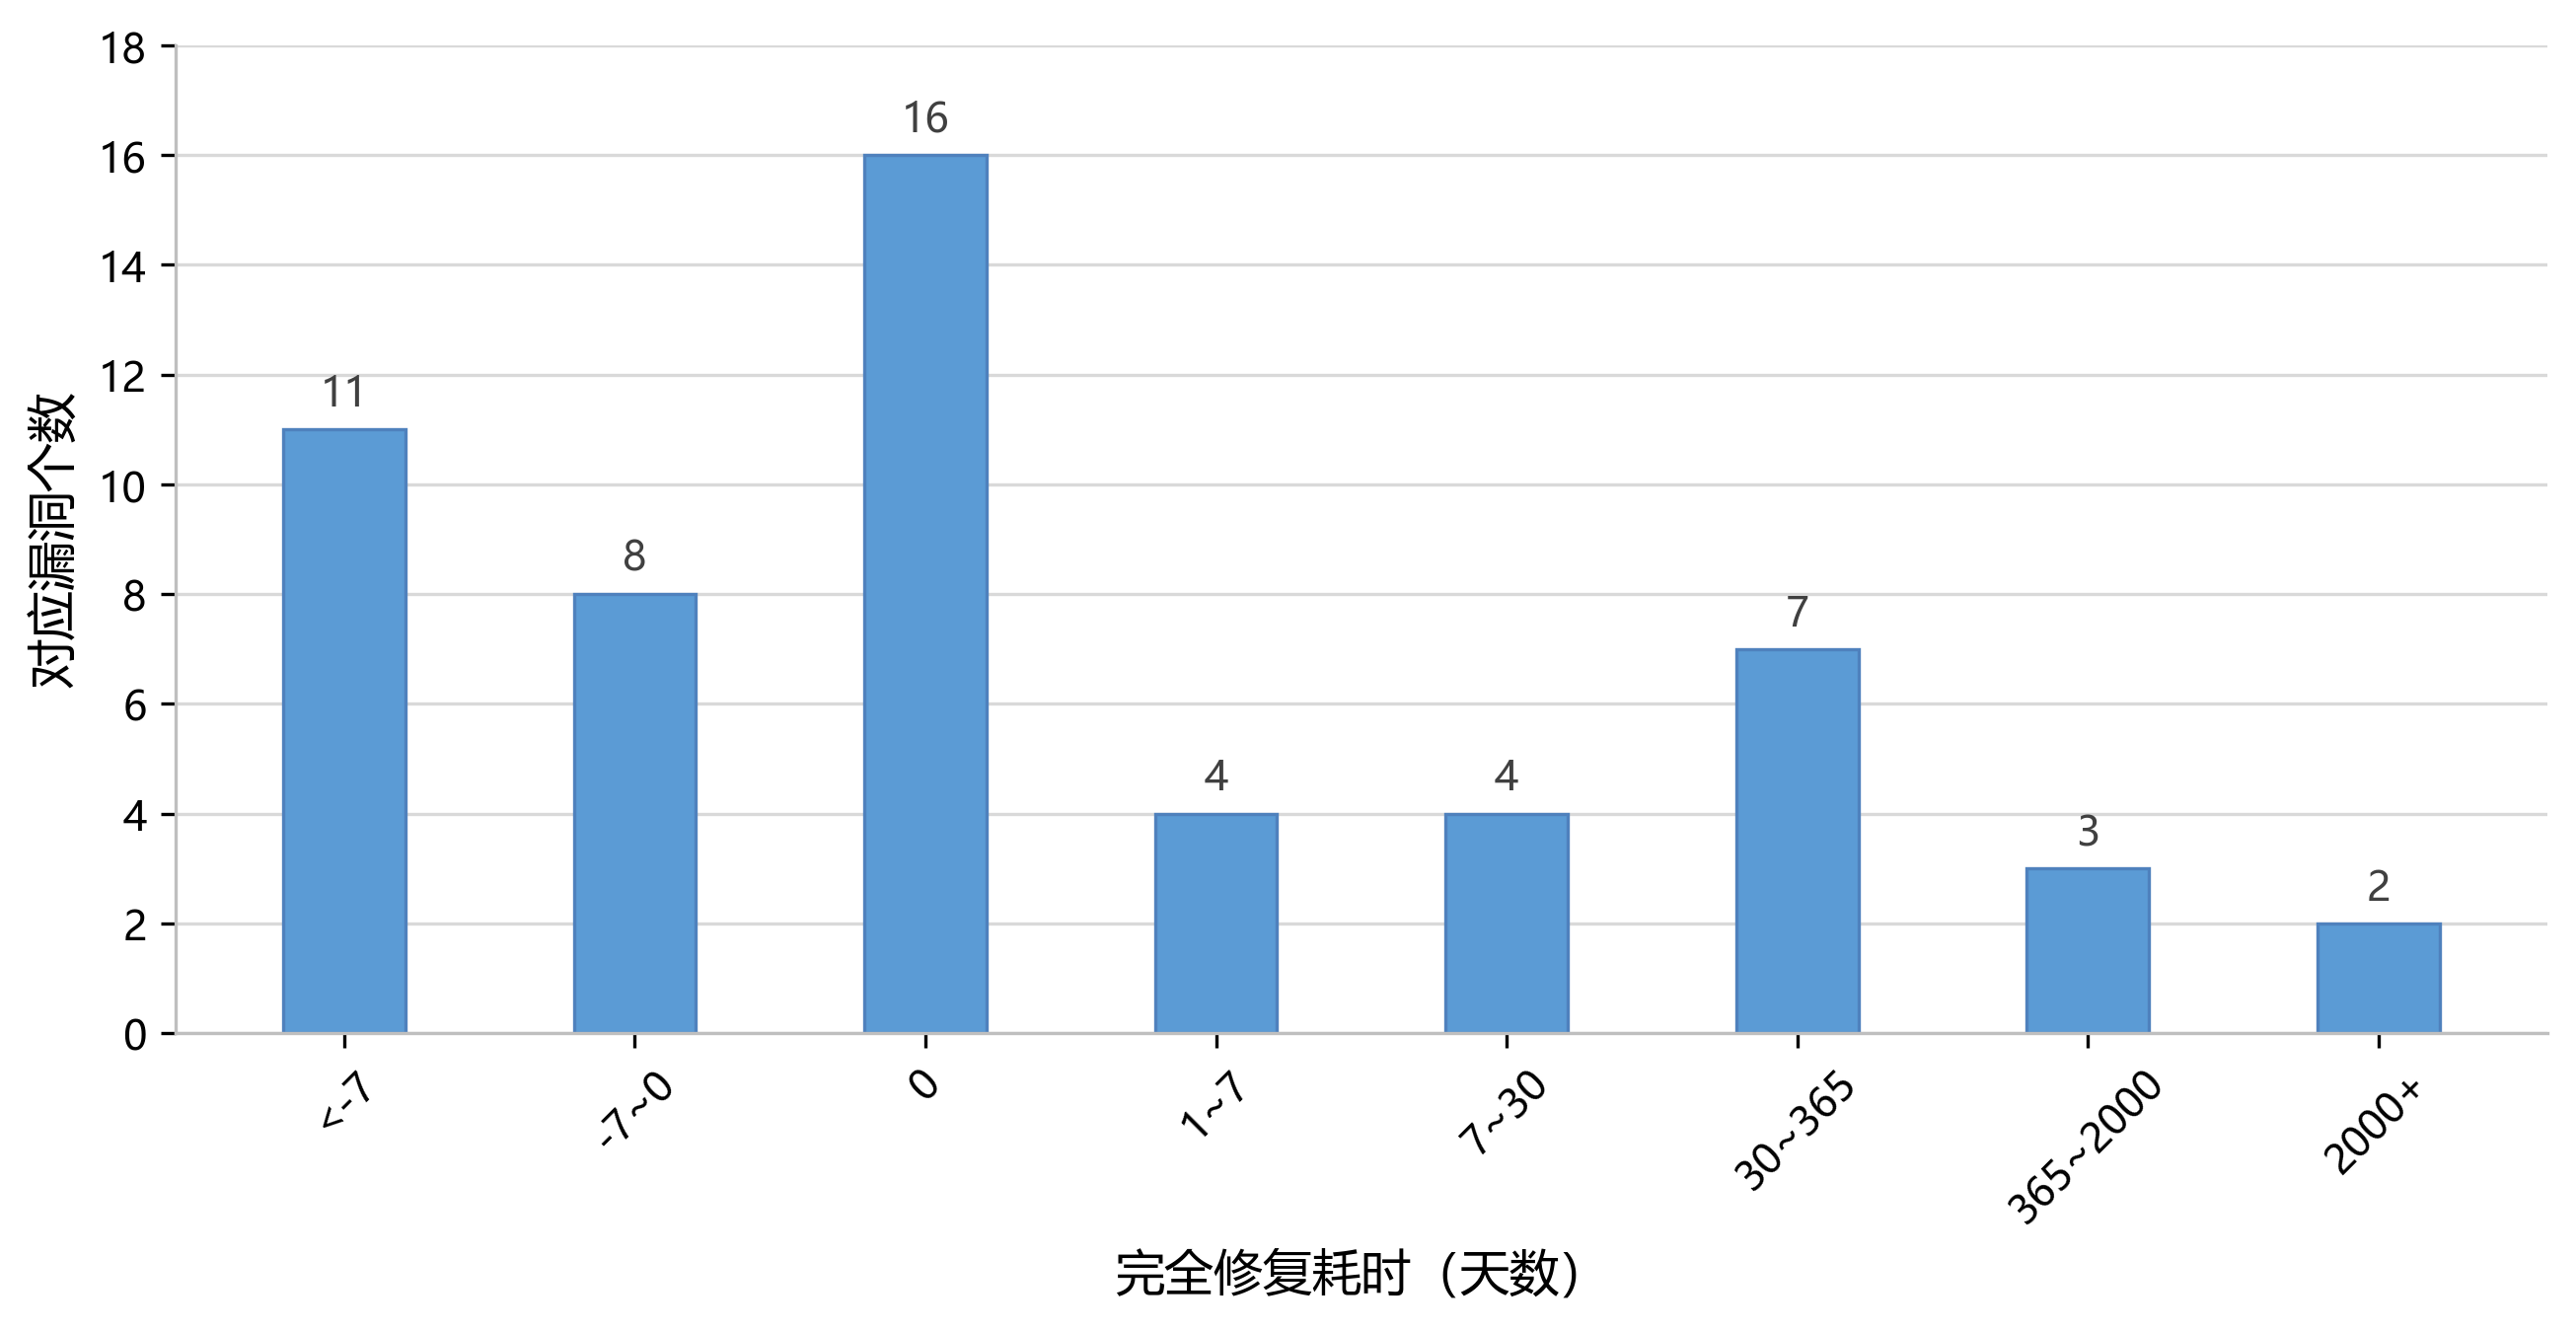
\includegraphics[width=0.8\textwidth]{images/cve-pub.png}
    \bicaption{云原生环境下权限提升漏洞的修复时间分布}{Distribution of remediation time for privilege escalation vulnerabilities in cloud-native environments}\label{fig:patch-window}
\end{figure}

这一处置任务的难点在于，临时防控策略并不能直接从 $\mathrm{CVE}$ 编号或简短公告中得到。权限提升漏洞往往同时涉及 $\mathrm{RBAC}$ 权限配置\cite{ferraiolo1995role}、控制平面交互、工作负载部署方式、运行时行为和网络可达关系等多个层面，并常与过度授权\cite{yang2023take}、授权检查缺陷、敏感信息泄露\cite{kubeguard_icws2025}等问题交织出现。真正有用的处置依据，通常分散在漏洞公告、修复提交、Issue/PR 讨论、配置清单与相关代码之中。要在较短时间内形成有效策略，需要先重建漏洞语义，再识别关键控制点，并据此判断应采用准入控制、$\mathrm{RBAC}$ 收敛、运行时监控还是网络隔离等措施。换言之，这里面对的不是单一规则编写问题，而是面向具体漏洞的证据组织与控制路径选择问题。

围绕云原生安全治理，现有工具已经覆盖了较完整的风险管控周期。静态层面，已有方法可对镜像依赖与 $\mathrm{Kubernetes}$ 清单进行扫描\cite{shamim2025prescription,k8smanifests2023}；动态层面，则包括基于 $\mathrm{eBPF}$ 的运行时观测与审计\cite{falco2025}、$\mathrm{OPA/Gatekeeper}$\cite{opa2025} 和 $\mathrm{Kyverno}$\cite{kyverno2025} 等准入控制机制，以及通过网络策略约束横向连通范围的防护手段\cite{Minna_2021,Budigiri_2021}。这些技术为集群安全提供了必要基础，但大多围绕通用基线核查和既有规则模式展开，更擅长识别普遍性风险；当目标转向某一具体漏洞时，它们往往缺少从多源证据出发、围绕利用条件组合控制措施的能力。实践中真正欠缺的，并不是新的单点工具，而是能够将已有工具与漏洞证据关联起来、面向补丁窗口期快速输出针对性临时策略的方法。

正是在这一点上，大语言模型提供了新的实现可能。其价值并不在于替代扫描器、准入控制器或运行时系统，而在于能够对异构文本与半结构化材料进行理解、归纳与重组，从中提取攻击语义、受影响对象与潜在控制点。如果将这种能力与现有安全工具的检测、约束和执行能力结合起来，便有机会形成一条从漏洞证据整理到策略生成、再到部署验证的协同处置路径。因此，本文的出发点并不是构造一种脱离现有生态的全新安全工具，而是探索如何将 $\mathrm{LLM}$ 与既有安全工具有效衔接，使其共同服务于补丁窗口期内的临时防控任务。

若要使这一思路真正落到可执行的方法设计上，还需要进一步回答以下三个问题。

\noindent\hangindent=1em\hangafter=1 (1) \textbf{如何构建面向具体漏洞的安全上下文}。权限提升漏洞的关键信息分散在代码仓库、漏洞公告、Issue/PR 讨论与修复提交等多类来源中。若缺乏统一的组织方式，模型很难准确把握漏洞成因、利用前提与影响边界。因此，方法首先需要建立可检索、可追溯的领域知识支撑，将分散证据转化为可供生成环节直接使用的安全上下文。

\noindent\hangindent=1em\hangafter=1 (2) \textbf{如何将漏洞语义映射为可部署的控制措施}。即便能够理解漏洞语义，临时防控策略的形成仍需要回答“在哪个控制面介入、采用何种约束方式、如何与现有工具配合”这一系列问题。也就是说，方法设计不仅要完成文本层面的归纳，还要把漏洞语义进一步转化为面向 Kubernetes 控制面的具体策略表达。

\noindent\hangindent=1em\hangafter=1 (3) \textbf{如何控制生成结果的不确定性}。大语言模型在将漏洞语义转化为策略代码时，仍可能出现幻觉、逻辑矛盾或偏离实际环境的问题。若缺乏有效的验证与校正机制，生成结果不仅可能无法阻断攻击，还可能干扰正常业务。因此，方法还必须考虑如何通过多阶段协同、结果评审与反馈优化，提高策略的有效性、无干扰性与可部署性。

基于上述动机，本文选择以多智能体协同方式组织整个防控流程，将证据整理、漏洞分析、策略生成、结果评审与反馈优化拆分为相互衔接的处理环节。这样的设计既服务于补丁窗口期内的快速响应需求，也为异构知识融合和生成结果控制提供了可操作的实现路径。后续内容将围绕这一思路，依次说明方法框架中的关键对象、知识支撑机制、协同生成流程以及质量控制方法。

\section{方法框架}

基于前文提出的现实需求，本文将补丁窗口期内云原生权限提升漏洞的防控问题建模为面向具体漏洞生成临时策略的自动化过程。按照控制手段的作用方式，相关措施可概括为监控策略与防护策略两个互补层次。其中，防护策略侧重在漏洞利用发生前阻断关键条件并收敛攻击面；监控策略侧重对运行时异常行为进行持续观测、告警与取证。围绕这两个目标，本文构建了基于多智能体安全策略管理的智能化漏洞防控框架。

\begin{figure}[htb]
    \centering
    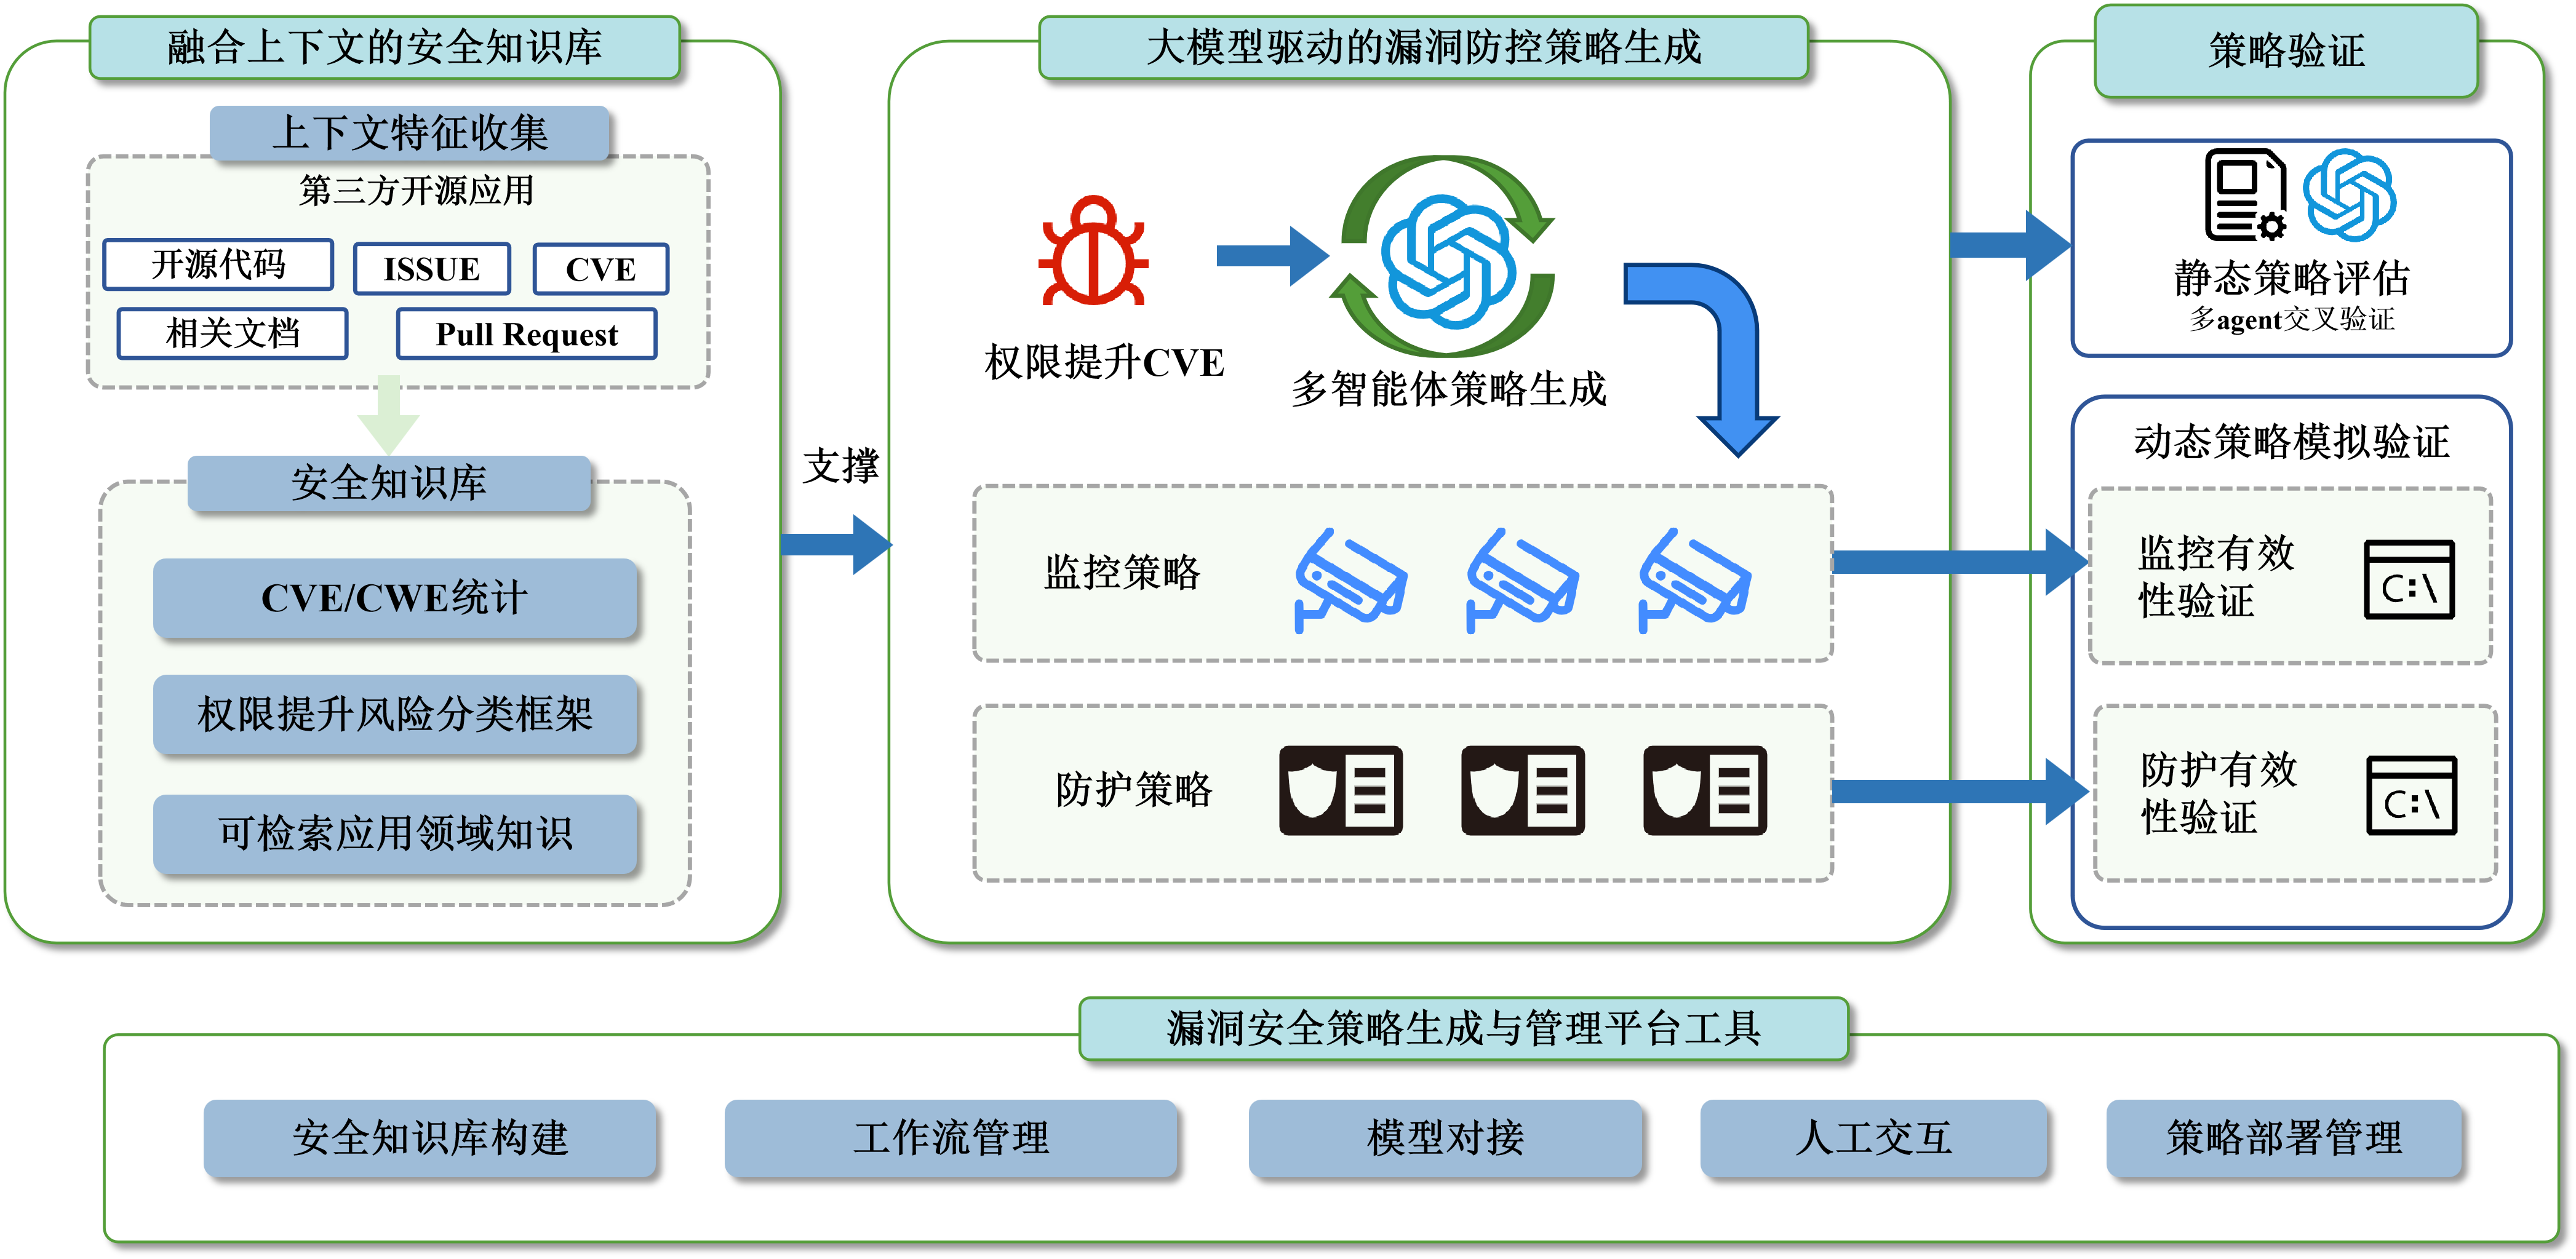
\includegraphics[width=1\textwidth]{images/总体框架.png}
    \bicaption{基于多智能体的策略化漏洞防控研究总体框架}{Overall multi-agent framework for strategy-based vulnerability prevention and control based on large language models}\label{fig:overall-framework}
\end{figure}

如图~\ref{fig:overall-framework}所示，该框架以权限提升类 $\mathrm{CVE}$ 为输入，依托大语言模型与多智能体协同，结合检索增强生成、思维链推理与反馈优化等技术，围绕安全知识支撑、策略生成、策略验证和平台工具建设，形成从漏洞披露到输出结构化 JSON 临时防控策略的自动化流程。具体而言，系统首先从代码仓库、漏洞公告、Issue/PR 讨论与补丁提交中提取多源证据，构建可追溯的漏洞安全知识库；随后通过安全知识、漏洞分析、策略生成、策略评审与策略优化等智能体协同，将漏洞语义转化为面向 Kubernetes 平台的监控与防护策略；最后结合质量评价与平台工具，实现结果排序、人工复核与部署验证。下面将依次对该流程涉及的对象定义、知识支撑机制、生成方法与评价过程展开说明。

\subsection{基本概念定义}

\subsubsection{基本对象} % 增加编号

为形式化描述面向漏洞的安全策略生成问题，本文将方法中的核心对象抽象为漏洞实例、安全上下文与安全策略三类实体。本文涉及的主要记号与核心术语已在前置部分的符号清单与术语表中汇总，这里仅给出与方法定义直接相关的形式化说明。记候选策略全集为 $\Pi$。策略质量评价所涉及的维度与记号将在下一小节中进一步给出。

\textbf{定义 1（漏洞实例）}。设 $\mathcal{V}$ 为漏洞实例空间。任一漏洞实例表示为
\[
v=\langle \mathit{id},\,d,\,m \rangle\in\mathcal{V}
\]
其中，$\mathit{id}$ 为漏洞标识符（如 CVE 编号），$d$ 为漏洞描述文本，$m$ 为与漏洞相关的元数据，用于刻画其严重性、受影响组件及版本范围等属性。

\textbf{定义 2（安全上下文）}。给定漏洞实例 $v$，其安全上下文 $c\in\mathcal{C}$ 定义为带来源标识的有限证据集合：
\[
c = \bigl\{\,\langle t_i,\,\mathit{src}_i \rangle \mid i\in[n_c] \,\bigr\}
\]
其中，$t_i$ 表示证据内容，$\mathit{src}_i$ 表示来源标识（如文档路径、公告链接或代码位置）。该定义强调上下文不仅提供与漏洞相关的背景事实，而且保留事实来源，以支撑后续策略生成与结果复核。

\textbf{定义 3（安全策略）}。针对给定漏洞实例 $v$ 的完整安全策略表示为三元组
\[
\pi = \langle \mathit{type},\;\mathit{method},\;\mathit{action} \rangle
\]
其中，$\mathit{type}\in\{\mathrm{mon},\mathrm{prot}\}$ 表示策略属于监控型还是防护型；$\mathit{method}=(m_1,\ldots,m_k)$ 表示控制机理序列，$\mathit{action}=(a_1,\ldots,a_k)$ 表示与之对应的执行表达序列。二者满足一一对应关系，即每个 $m_i$ 均对应一个可部署的 $a_i$，共同构成完整的防控措施单元。

对给定漏洞实例 $v$，生成阶段得到的候选策略集合记为 $\Pi_v\subseteq\Pi$。


\subsubsection{质量评价指标}

由于不同漏洞样本在业务环境、证据完备程度与候选策略规模上存在差异，若直接采用绝对分值，容易引入尺度漂移与比较偏置。与此同时，监控策略与防护策略在优化目标上并不完全同质，前者更强调观测、告警与取证能力，后者更强调阻断、收敛与约束效果。因此，本文在评价阶段先按策略类型划分候选集合，再在各自子集中实施基于排序的相对评价。记类型集合为 $\mathcal{T}=\{\mathrm{mon},\mathrm{prot}\}$，对任意 $\tau\in\mathcal{T}$，定义
\[
\Pi_v^{\tau}=\Pi_v\cap\Pi_{\tau}
\]
表示漏洞实例 $v$ 在类型 $\tau$ 下的同质候选子集。下文若不强调策略类型，统一用 $\Pi_v$ 表示漏洞实例 $v$ 的候选策略集合；当需要区分监控型与防护型时，再使用 $\Pi_v^{\tau}$ 表示对应子集。记评价维度集合为 $\Delta=\{E,I,D\}$，分别对应有效性、无干扰性与可部署性。

\textbf{定义 4（三维质量向量）}。策略质量由映射 $q\colon\Pi\to[0,1]^3$ 给出：
\[
q(\pi) = \bigl(E(\pi),\;I(\pi),\;D(\pi)\bigr)
\]
其中，$E$ 衡量策略对主要攻击路径与关键风险面的覆盖程度，$I$ 衡量策略对正常业务的扰动程度及误报风险，$D$ 衡量策略在现有环境中的落地难度与执行清晰度。

\subsection{云原生权限提升安全知识库}

如图~\ref{fig:cve-database}所示，本节围绕漏洞实例 $v$ 构建可追溯云原生权限提升安全知识库 $\mathcal{K}_v$，并通过检索形成安全上下文 $c$，为后续策略生成提供带来源标识的证据支撑。

\begin{figure}[htb]
    \centering
    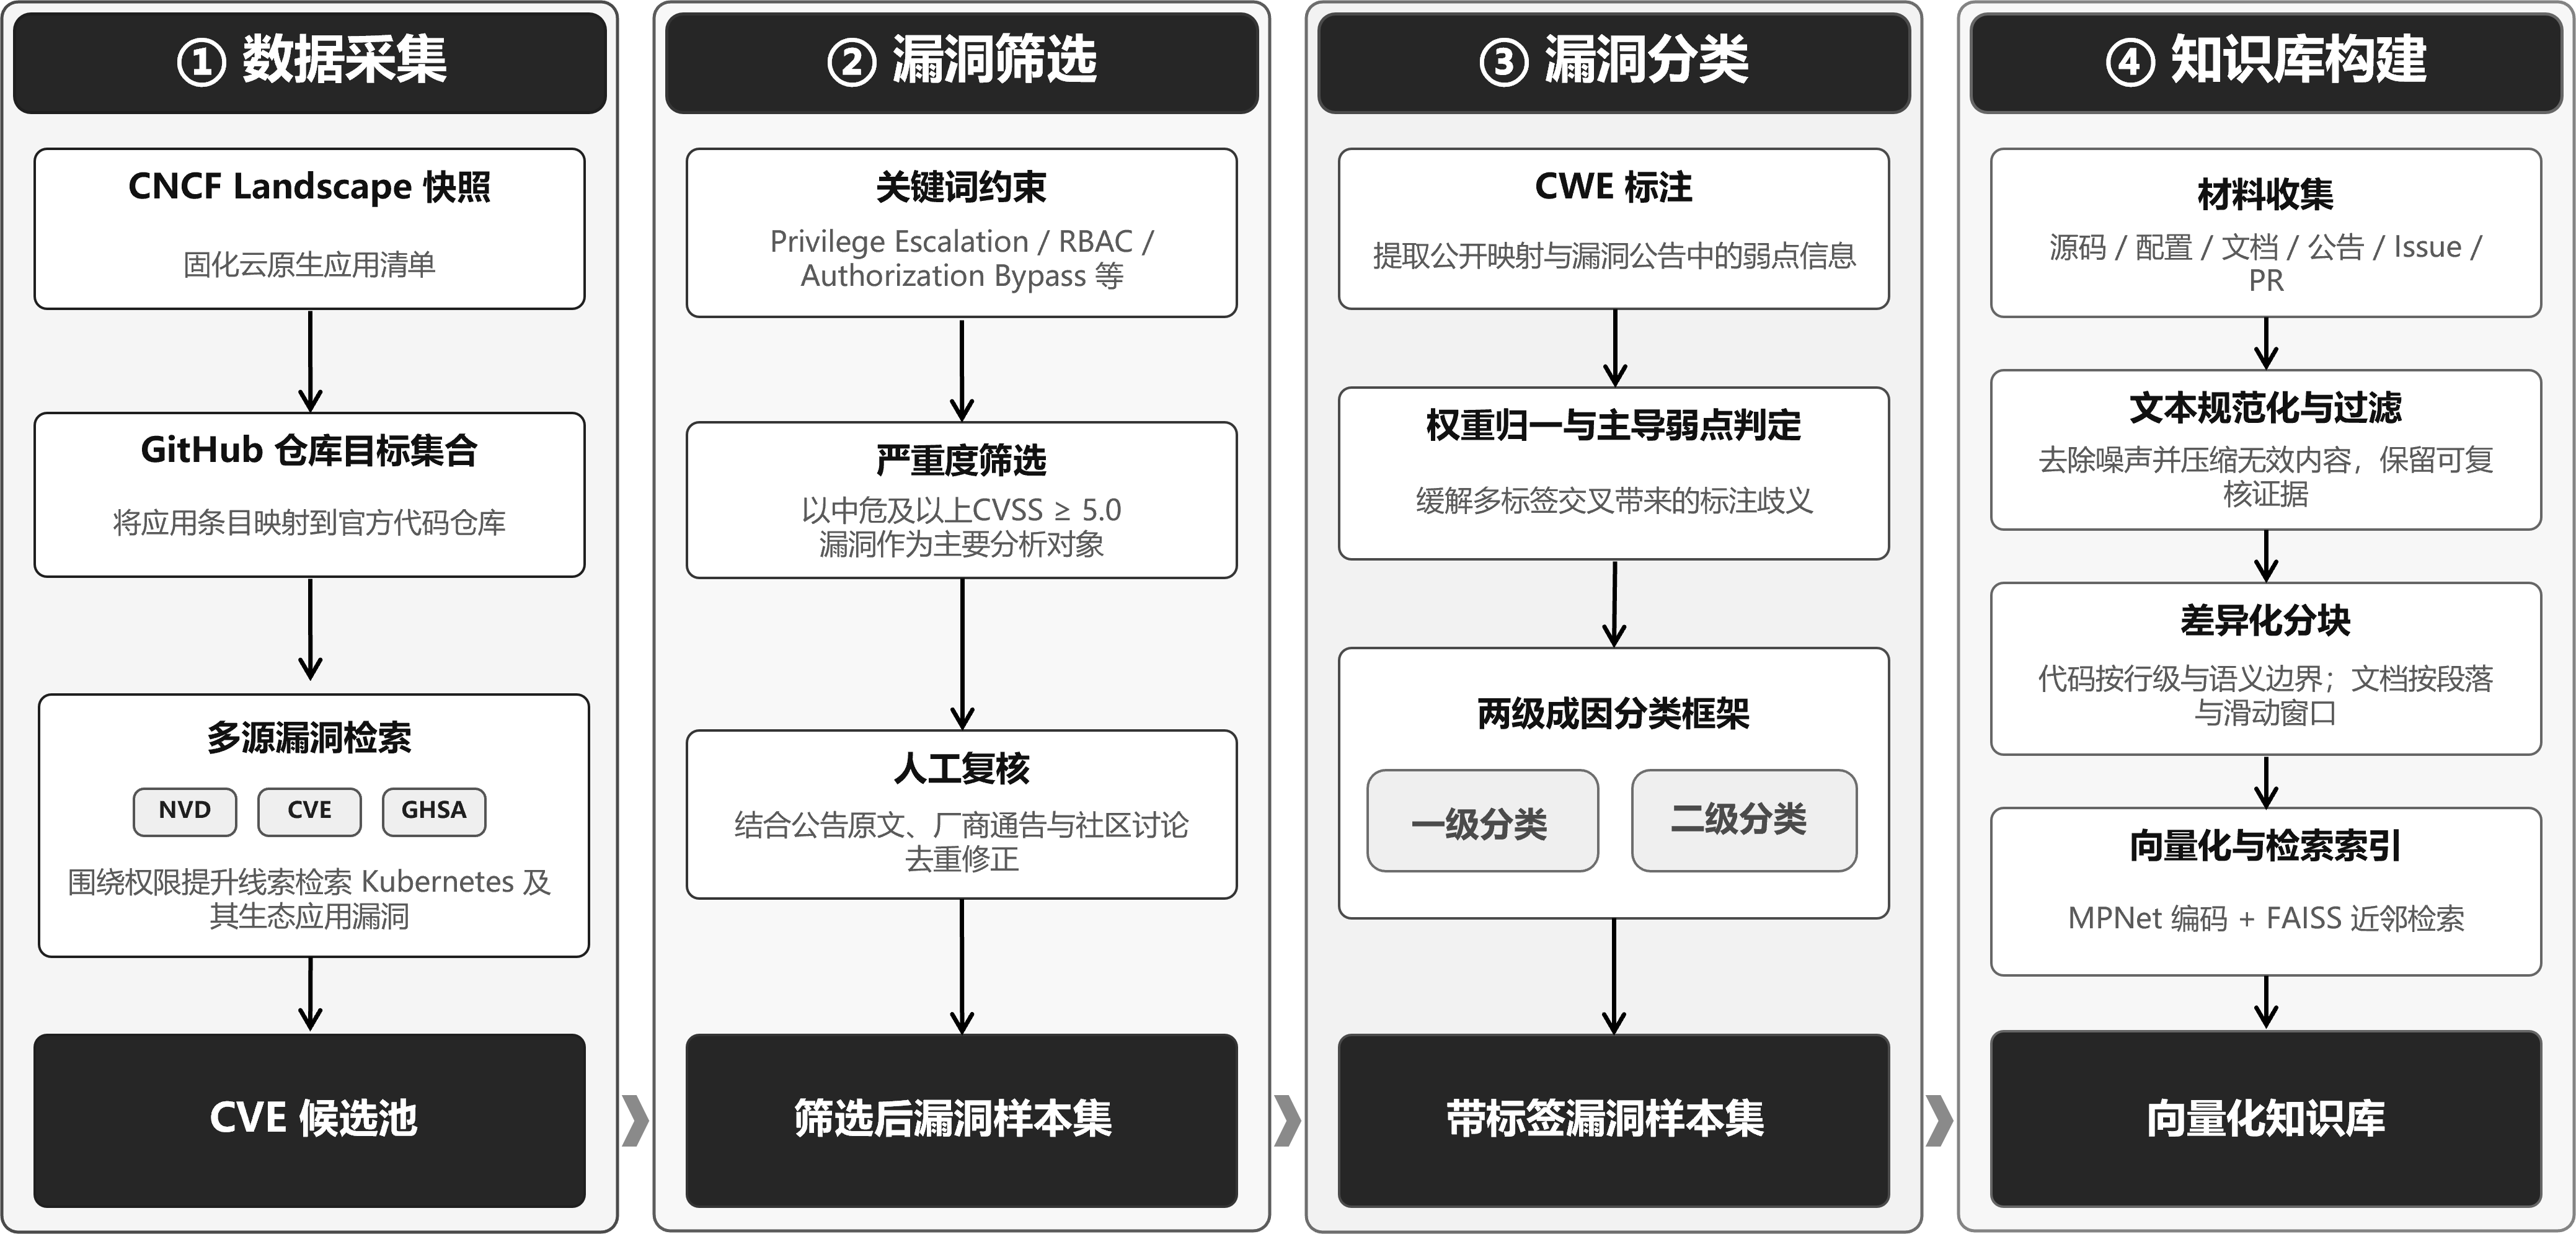
\includegraphics[width=0.92\textwidth]{images/chap3_cve_database.png}
    \bicaption{云原生权限提升漏洞知识库构建}{Overview of the cloud-native privilege escalation vulnerability knowledge base construction}\label{fig:cve-database}
\end{figure}


\subsubsection{数据采集}

本文以 Kubernetes 及其生态开源应用为研究对象，首先从 CNCF Landscape 获取云原生应用清单，并对清单进行快照固化，以保证采集过程可复现。随后，将清单条目名称映射到其官方代码仓库，形成后续漏洞检索与证据收集的目标集合。

在此基础上，本文综合使用 NIST NVD\footnote{NIST NVD（National Vulnerability Database）：\url{https://nvd.nist.gov/}}、MITRE CVE 官方库\footnote{MITRE CVE：\url{https://cve.mitre.org/}}与安全公告平台 GitHub Security Advisory\footnote{GitHub Security Advisory：\url{https://github.com/advisories}}三个来源，围绕权限提升线索对 Kubernetes 及其生态应用开展多源漏洞检索，获得初步 CVE 候选池。

\subsubsection{漏洞筛选}

为从 CVE 候选池中筛选出高质量样本，本文采用关键词约束、严重性阈值与人工复核相结合的三重过滤策略：
\begin{itemize}
    \item \textbf{关键词约束}：在 CVE 描述与参考链接中匹配 Privilege Escalation、Authorization Bypass、Improper Access Control、RBAC、ServiceAccount、ClusterRole、Container Escape/Sandbox Escape/Breakout 等关键词；
    \item \textbf{严重性阈值}：采用 CVSS v3.x 评分，并以 $\geq 5.0$ 的中危及以上漏洞为主要对象；
    \item \textbf{人工复核}：对候选条目结合公告原文、厂商通告与社区讨论进行复核，剔除重复或与权限提升无关的记录，并补全攻击前提、影响面与可用缓解信息。
\end{itemize}
最终保留的结构化字段包括 CVE 编号、漏洞摘要、披露时间、受影响组件与版本范围、修复版本、CVSS 评分、参考链接，以及与修复相关的补丁提交记录等。上述字段与漏洞实例 $v=\langle \mathit{id},\,d,\,m \rangle$ 直接对应：CVE 编号即标识符 $\mathit{id}$，漏洞摘要构成描述 $d$，其余属性如严重性评分、受影响版本和参考链接等共同构成元数据 $m$。

为保证数据构建过程可复现，本文对同一批次样本采用统一快照方式完成采集，并在构建配置中记录应用清单快照、检索时间窗口、纳入与剔除准则以及去重规则。对于来自不同数据源但指向同一漏洞事实的记录，以 CVE 编号为主键进行合并；对于无独立编号但经公告与补丁信息确认指向同一漏洞事件的记录，则视为重复项而不重复计数。

\subsubsection{漏洞分类}

漏洞样本的分类方式直接影响后续策略生成的针对性。为此，本文构建了面向策略生成场景的两级成因分类框架，旨在为模型提供稳定且可解释的风险语义线索，从而约束推理路径、辅助关键控制点与实施路径的选择，提升输出策略的可部署性、可验证性与副作用可控性。

首先，本文依据公开映射与公告信息提取每个 CVE 的 CWE（Common Weakness Enumeration）标签，并统计不同 CWE 的出现频次。CWE 是 MITRE 维护的软件弱点枚举体系，可用于将具体 CVE 归并到更抽象的弱点类型。

\begin{figure}[htb]
    \centering
    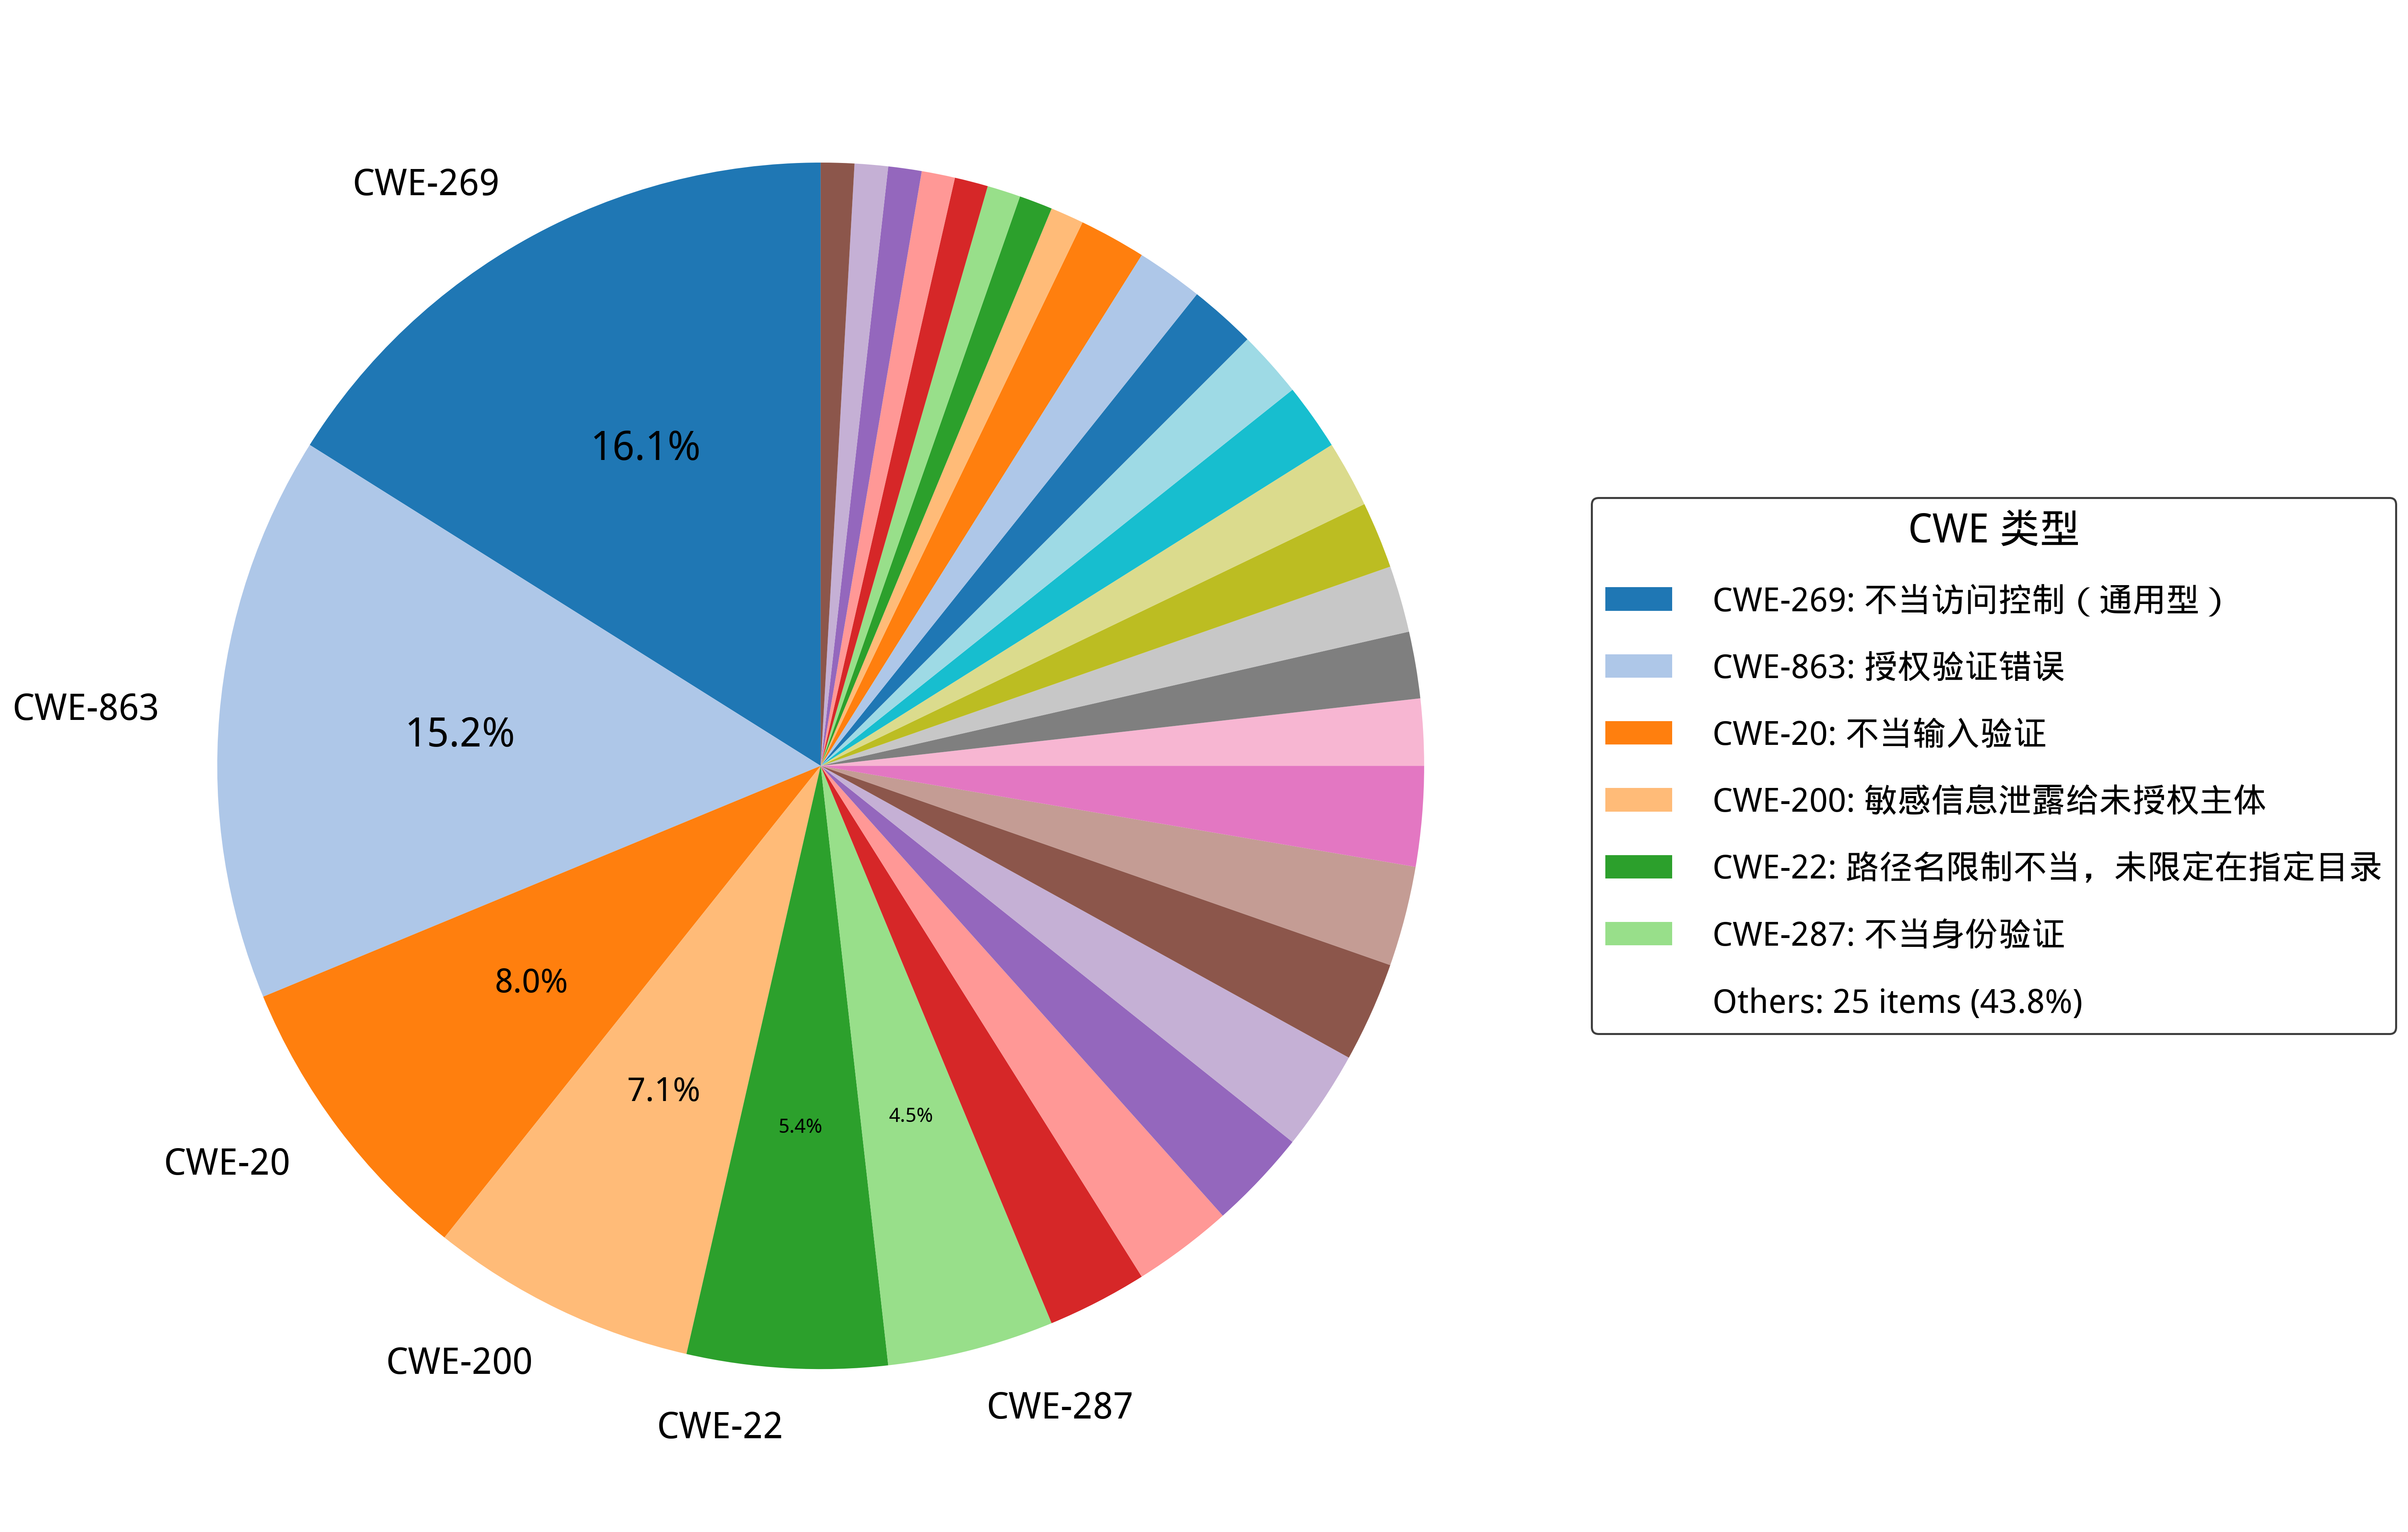
\includegraphics[width=1\textwidth]{images/cwe_distribution_pie.png}
    \bicaption{Kubernetes 权限提升 CVE 对应的 CWE 类型占比}{Distribution of CWE categories corresponding to Kubernetes privilege escalation CVEs}\label{fig:cwe-distribution-ch3}
\end{figure}

CWE 体系并不是严格互斥的分类框架。同一漏洞往往会同时对应多个弱点条目，不同条目在抽象层次上也可能彼此交叉。在本文收集的 55 个权限提升漏洞中，有 20 个样本同时关联两个及以上 CWE 标签，占比 36\%。为更客观地反映 CWE 分布，统计时令每个 CVE 的总权重为 1，多标签样本按标签数平均分配。结果表明，授权不当、权限管理不当等访问控制类弱点常与输入验证不当等问题同时出现，这说明权限提升漏洞通常具有复合成因。仅依赖单一 CWE 标签，难以为后续防控策略提供稳定的语义约束，因此有必要进一步构建面向防控动作的成因分类框架。

基于这一问题，本文进一步提出面向云原生权限提升漏洞的两级成因分类框架，并为每个漏洞确定一级类和二级类标签。一级分类用于概括高层风险来源，如安全逻辑缺陷、配置缺陷、代码注入和敏感信息泄露；二级分类则进一步细化到更贴近防控动作选择的类型，如授权验证不完善、默认不安全配置等。经过这样的整理，漏洞分析结果可以更自然地映射到 RBAC 最小权限、准入控制、网络隔离、运行时策略与审计等具体控制点。

在策略生成阶段，分类结果作为提示词中的结构化约束，引导模型先识别漏洞的主要成因，再定位关键控制点，最后组织可执行的防控动作，从而减少泛化建议和无关信息，提高策略的针对性与可部署性。完整的一级、二级分类及其与 CWE 的对应关系见附录表~\ref{tab:vuln-cwe-mapping}。

为降低多标签条件下的标注歧义，本文对每个样本只保留一个主导的一级类和二级类标签。判定时优先选择直接造成权限边界突破的成因；其余伴随弱点仍保留在 CWE 映射表中，作为补充语义信息。对于边界不清或存在多种解释路径的样本，再结合漏洞公告、修复补丁语义与攻击路径描述进行复核后裁决。

\begin{table}[htb]
    \centering\bicaption{云原生权限提升漏洞分类框架（CWE 对应详见附录表~\ref{tab:vuln-cwe-mapping}）}{Classification framework for cloud-native privilege escalation vulnerabilities (see Appendix Table~\ref{tab:vuln-cwe-mapping} for the CWE mapping)}\label{tab:cloud-native-vuln}
    \small
    \setlength{\tabcolsep}{3pt}
    \noindent\renewcommand{\arraystretch}{0.9}

    \begin{tabular}{ >{\centering\arraybackslash}p{3cm} >{\raggedright\arraybackslash}p{3cm} >{\raggedright\arraybackslash}p{3cm} }
        \toprule
        \textbf{一级分类} & \textbf{二级分类} & \textbf{示例 CVE} \\
        \midrule
        \multirow{2}{*}{配置缺陷} & 冗余权限 & \mbox{CVE{-}2023{-}30512} \\
         & 网络隔离不足 & \mbox{CVE{-}2020{-}4062} \\
        \midrule
        \multirow{4}{*}{安全逻辑缺陷} & 访问控制缺陷 & \mbox{CVE{-}2022{-}24768} \\
         & 身份验证绕过 & \mbox{CVE{-}2023{-}22482} \\
         & 输入验证不足 & \mbox{CVE{-}2023{-}3955} \\
         & 授权验证不完善 & \mbox{CVE{-}2022{-}21701} \\
        \midrule
        \multirow{3}{*}{敏感信息泄露} & API端口暴露 & \mbox{CVE{-}2022{-}1902} \\
         & 日志泄露 & \mbox{CVE{-}2019{-}10165} \\
         & 配置文件泄露 & \mbox{CVE{-}2019{-}3869} \\
        \midrule
        \multirow{2}{*}{代码注入} & 命令注入 & \mbox{CVE{-}2021{-}41254} \\
         & 路径遍历 & \mbox{CVE{-}2022{-}24877} \\
        \bottomrule
    \end{tabular}
\end{table}

以下对各一级分类分别展开说明。

\textbf{配置缺陷}指应用或基础设施的配置不当导致的安全漏洞，主要包括两种情形：
\begin{itemize}
    \item 过度权限配置：Kubernetes RBAC 配置不当、Role/ClusterRole 规则范围过宽或绑定关系不合理等，使低权限主体获得超出其职责的资源访问与高危操作能力。该类问题在第三方应用接入场景中尤为常见，并已被证明可被用于接管集群关键资源\cite{o1995redundant,yang2023take}。
    \item 网络隔离不足：容器、Pod或服务间缺乏网络隔离，导致攻击者可以横向移动获取其他权限。
\end{itemize}

\textbf{安全逻辑缺陷}指应用代码中的安全机制设计或实现不当，涵盖以下情形：
\begin{itemize}
    \item 访问控制缺陷：应用的权限检查不完全或存在逻辑漏洞，允许绕过权限验证；
    \item 身份验证绕过：认证机制设计缺陷，攻击者可以冒充他人身份或跳过认证步骤；
    \item 输入验证不足：对请求参数、资源标识或边界条件的校验不充分，导致攻击者借由异常输入扩大权限边界或触发越权路径；
    \item 授权验证不完善：权限检查在某些操作路径或边界条件下缺失。
\end{itemize}

\textbf{敏感信息泄露}指重要的身份、密钥或权限信息意外暴露，常见形式包括：
\begin{itemize}
    \item API 端口暴露：管理接口、内部 API 或调试端口未受保护暴露在网络上；
    \item 日志泄露：错误泄露的日志文件中包含密钥、命令历史等敏感信息；
    \item 配置文件泄露：配置文件包含硬编码的凭证或密钥。
\end{itemize}

\textbf{代码注入}指应用对用户输入的处理不当，使攻击者得以注入恶意代码，典型子类包括：
\begin{itemize}
    \item 命令注入：应用直接执行用户提供或可控的命令，攻击者可以执行任意系统命令；
    \item 路径遍历：应用文件访问检查不完整，攻击者可以访问系统其他部分的文件。
\end{itemize}

\subsubsection{知识库构建}

知识库构建阶段的目标是将与漏洞 $v$ 相关的多源材料组织为带来源标注的证据集合，并建立支持按需取证的检索能力。围绕 $v$ 构建知识库 $\mathcal{K}_v$ 后，策略生成阶段即可通过语义检索提取相关证据片段，并按需组装为安全上下文 $c$，为后续分析提供可追溯的事实依据。

具体而言，本文首先针对每个漏洞关联的开源应用仓库收集代码、配置与文档等可读文本，同时纳入与漏洞相关的安全公告、议题（Issue）/合并请求（Pull Request）讨论以及修复提交信息。随后，对文本进行最小化规范，并过滤超长或二进制内容，以降低噪声与资源开销。

在完成材料收集后，为兼顾证据粒度与可复核性，本文对不同材料采用差异化分块策略：对代码和配置按行切分，并尽量对齐函数或语义边界；对文档则按段落与窗口切分，并保留适当重叠，以减少跨块语义断裂。

在此基础上，为实现语义层面的证据召回，本文为每个文本块构造向量表示，并建立近邻检索索引。实验实现中，采用 \texttt{sentence-transformers} 框架中的 MPNet 句子编码器 \texttt{all-mpnet-base-v2} 完成文本表示\cite{reimers2019sentencebert,song2020mpnet}，并基于 FAISS\cite{douze2024faiss} 构建相似度索引。为保证可追溯性与可复现性，索引与元数据同步持久化，内容包括向量索引文件、块级元数据以及构建配置。块级元数据记录来源路径或链接、块 ID、块类型与范围等信息；构建配置记录分块参数与检索阈值等关键设置。

上述流程得到的向量知识库为后续策略生成提供了可追溯的证据供给能力。模型在推导控制措施时可以检索到与漏洞相关的关键事实与上下文片段，并通过来源标识完成快速定位与复核。

\subsection{基于多智能体协同的策略生成与优化}


策略生成阶段以漏洞实例 $v$ 与安全上下文 $c$ 为输入，产出候选策略集合 $\Pi_v\subseteq\Pi$。按照定义 3，每个候选 $\pi\in\Pi_v$ 都表示为三元组 $\pi=\langle \mathit{type},\mathit{method},\mathit{action}\rangle$。按策略类型划分，$\Pi_v^{\mathrm{mon}}=\Pi_v\cap\Pi_{\mathrm{mon}}$ 表示监控策略候选子集，$\Pi_v^{\mathrm{prot}}=\Pi_v\cap\Pi_{\mathrm{prot}}$ 表示防护策略候选子集。整个流程结合检索增强、思维链推理与反馈优化三类机制，由安全知识、漏洞分析、策略生成、策略评审与策略优化五类智能体分工完成：先整理证据，再形成结构化分析，随后生成候选，并依据评审反馈持续修订，以降低误报与运维噪声并提升可部署性。

\begin{figure}[htb]
    \centering
    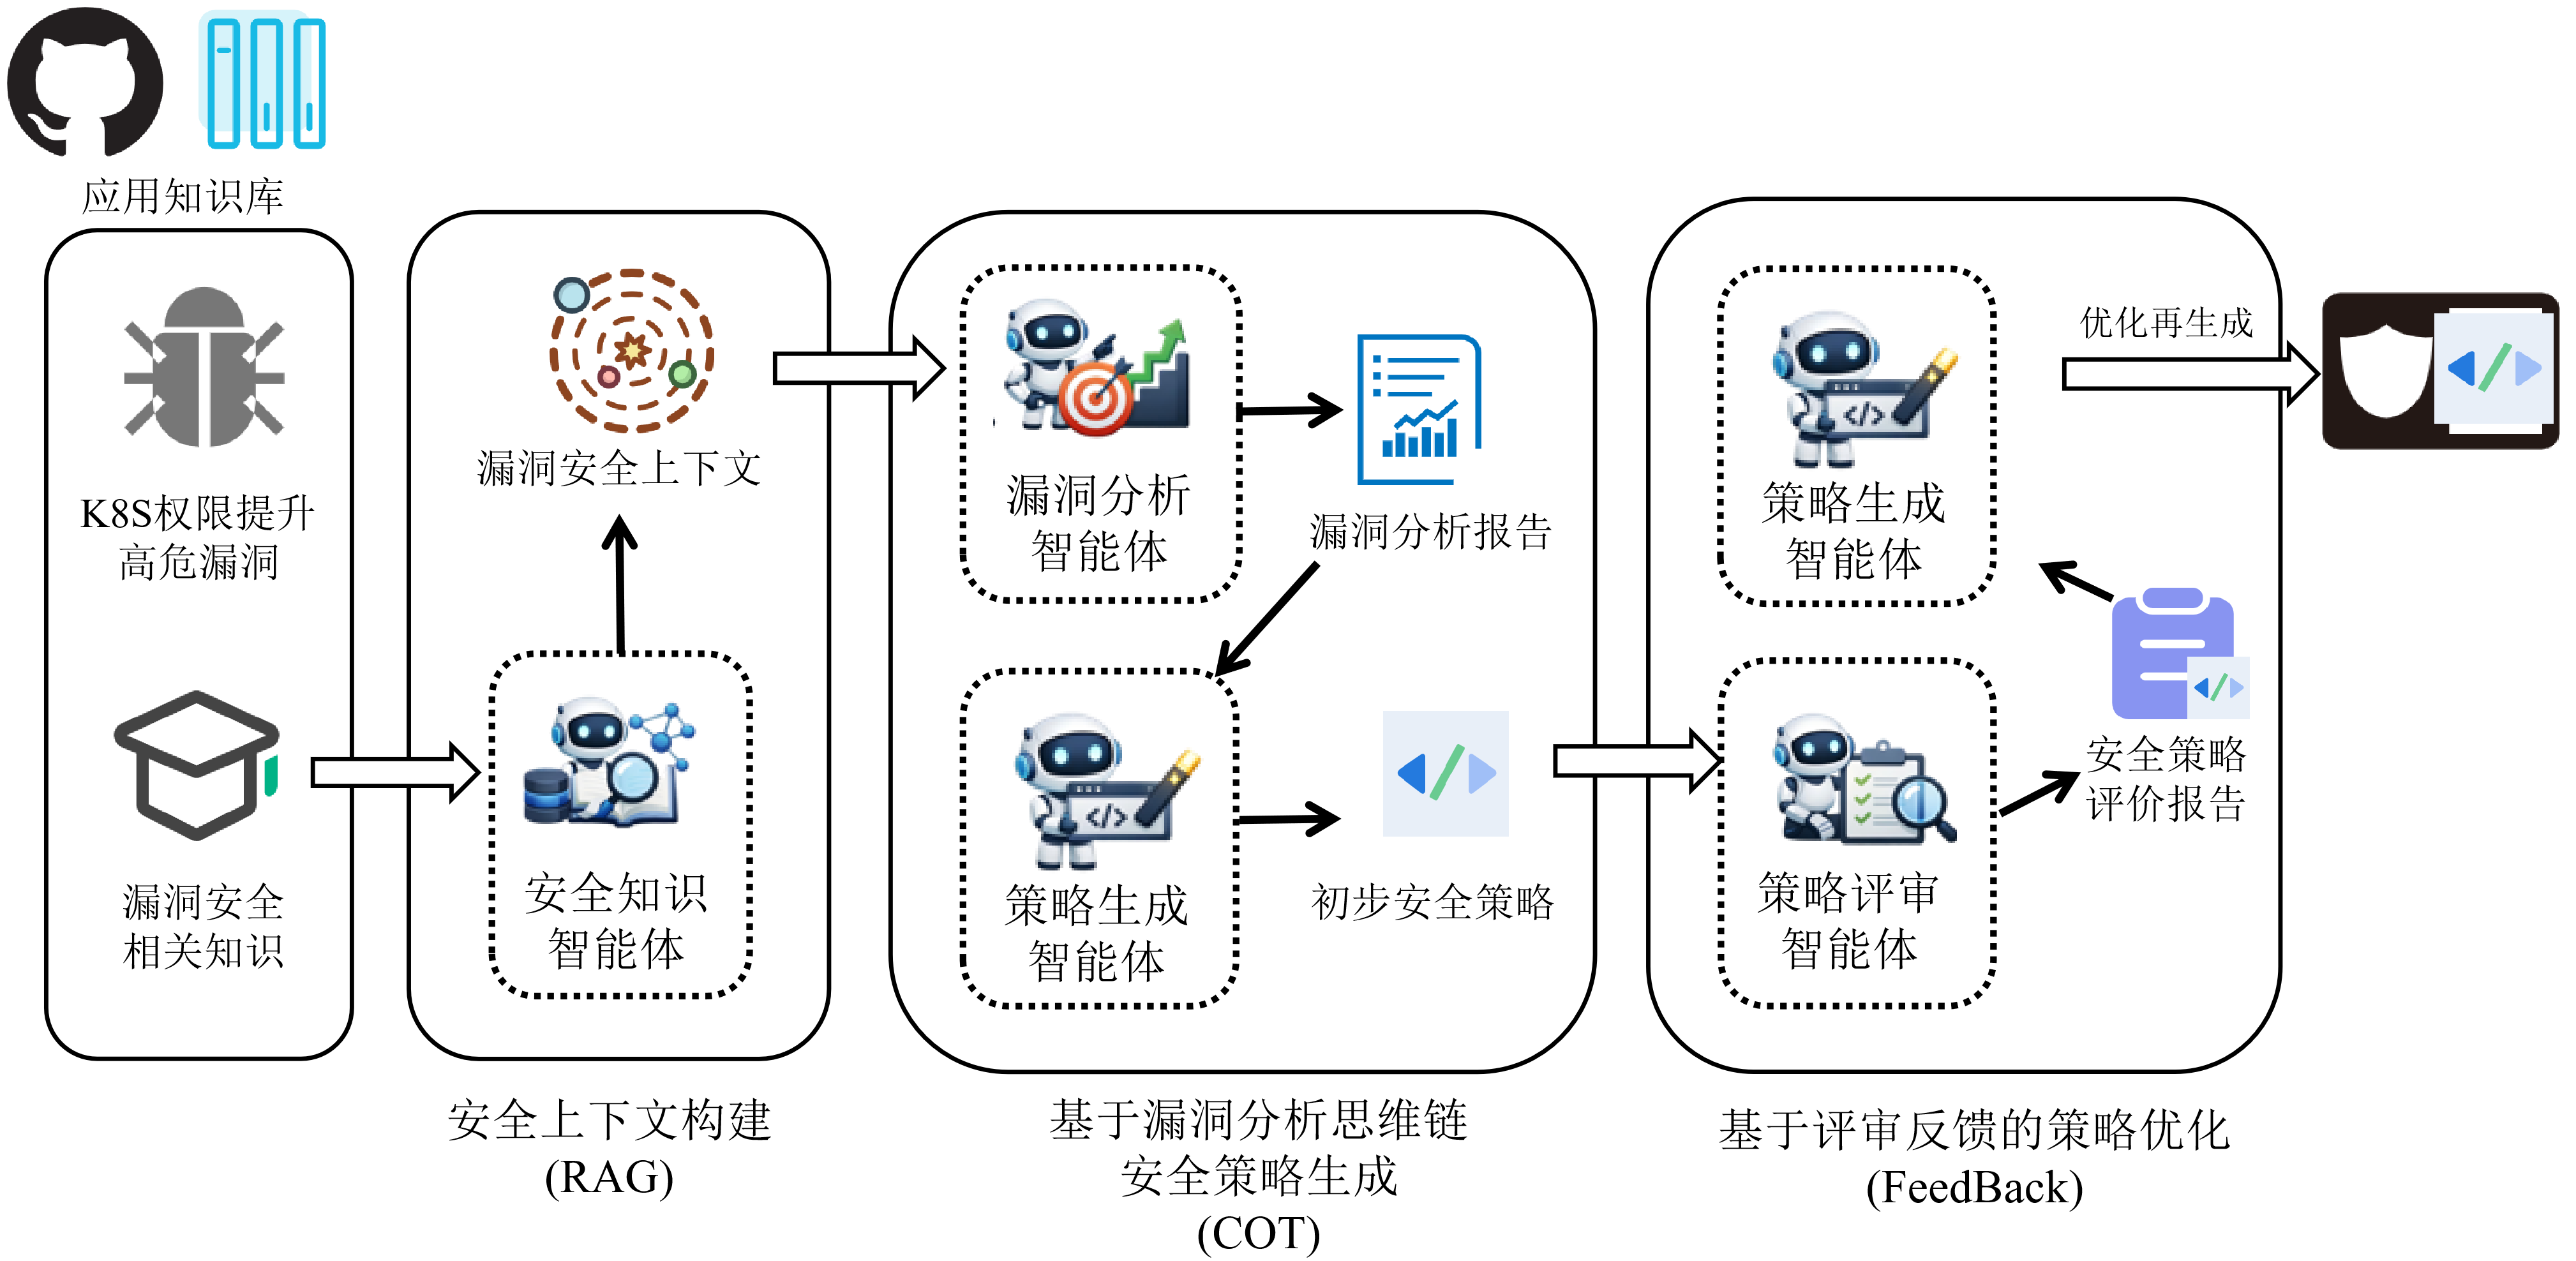
\includegraphics[width=1\textwidth]{images/method.png}
    \bicaption{多智能体协同的策略化漏洞防控工作流}{Multi-agent collaborative framework for strategy-based vulnerability prevention and control}\label{fig:method}
\end{figure}


\subsubsection{安全上下文构建}

安全上下文构建的关键在于保证证据可追溯。按照定义 2，证据集合记为 $c=\{\,\langle t_i,\mathit{src}_i\rangle\mid i\in[n_c] \,\}$。在知识库阶段，系统为每个片段记录来源元数据，如路径、URL、版本与位置；在生成阶段，再从知识库与安全材料中检索候选证据，并由\textbf{安全知识智能体}完成去重与提炼，输出触发条件、受影响组件、权限边界与可控点，同时保留对应的 $\mathit{src}_i$ 供复核。

为保证不同实验轮次中证据整理过程具有一致的输入输出边界，本文将该智能体的指令约束抽象为由角色、输入、任务和输出构成的四元模式，其在全流程中的统一定义见表~\ref{tab:agent-instruction-schema}。安全知识智能体的职责是将离散证据整理为带来源标识的结构化摘要，而不是直接给出策略建议。

\begin{PromptBox}{安全知识智能体提示词简化示例}
\begin{Verbatim}[breaklines,breakanywhere,mathescape=true]
你是云原生安全知识整理助手。
## 输入
漏洞实例 $v$ 与候选证据集合 $c$

## 任务
提炼受影响组件、触发条件、权限边界、攻击前提与缓解线索，
保留每条结论对应的来源标识。

## 输出
返回结构化证据摘要，不直接生成防控策略。
\end{Verbatim}
\end{PromptBox}

\subsubsection{基于漏洞分析思维链的策略生成}

本节将漏洞分析、技术选型与策略生成纳入统一的结构化约束，要求各环节输出可复核的中间结论。与仅给出自然语言建议相比，这种做法能够减少信息缺失与表述歧义。

首先，\textbf{漏洞分析智能体}基于漏洞摘要与安全上下文 $c$ 形成结构化分析结果，覆盖漏洞类型、攻击路径、影响范围与风险类别，并与前述成因分类体系保持一致。随后，\textbf{策略生成智能体}在结构化指令约束与分步推理引导下，根据分析结论选择控制手段并组织动作序列。具体而言，它会结合平台可用能力，在身份与权限收敛、网络隔离、运行时约束与准入控制等手段之间确定实施路径，并将其映射为最终策略对象；当证据不足以支持唯一结论时，则显式保留待补充信息与必要假设。为保持方法主线清晰，同时保证实验过程可复现，本文保留简化后的提示词示例，并以表~\ref{tab:agent-instruction-schema}概括各智能体的统一约束。

\begin{table}[htb]
    \centering
    \bicaption{多智能体指令约束摘要}{Summary of instruction constraints for the multi-agent workflow}\label{tab:agent-instruction-schema}
    \small
    \setlength{\tabcolsep}{3pt}
    \renewcommand{\arraystretch}{1.1}
    \begin{tabular}{>{\raggedright\arraybackslash}p{2.4cm} >{\raggedright\arraybackslash}p{3.0cm} >{\raggedright\arraybackslash}p{3.6cm} >{\raggedright\arraybackslash}p{4.0cm}}
        \toprule
        \textbf{智能体} & \textbf{输入} & \textbf{核心任务} & \textbf{输出约束} \\
        \midrule
        安全知识智能体 & 漏洞实例与候选证据片段 & 抽取受影响组件、触发条件、攻击前提、权限边界与缓解线索 & 输出带来源标识的结构化证据摘要 \\
        漏洞分析智能体 & 漏洞实例与安全上下文 & 形成漏洞类型、攻击路径、影响范围与风险类别的结构化分析 & 输出满足预定义模式的分析结果 \\
        策略生成智能体 & 中间分析结论、控制手段选择结果与安全上下文 & 生成监控或防护策略，并保持字段完整、一致且可验证 & 输出包含 \texttt{type}、\texttt{method} 与 \texttt{action} 的结构化策略对象 \\
        策略评审智能体 & 漏洞实例、候选策略集合与补充约束 & 从有效性、干扰风险与验证需求等方面形成评审意见 & 输出包含总体结论与逐策略点评的结构化评审结果 \\
        策略优化智能体 & 漏洞实例、候选策略集合与评审结论 & 吸收有效控制、剔除高噪声建议，并补齐前置条件与回滚边界 & 输出优化后策略及相对原候选的改进说明 \\
        评价智能体 & 匿名化与随机化后的同类型候选策略集合 & 在 $E$、$I$、$D$ 三个维度上给出严格排序 & 输出满足预定义模式的维度排序结果及必要判据 \\
        \bottomrule
    \end{tabular}
\end{table}

策略生成阶段需要在统一的数据模式下将分析结论映射为可部署的策略对象，因此除任务目标外，还需明确输出字段与约束边界。表~\ref{tab:agent-instruction-schema}中漏洞分析与策略生成两类智能体的约束，共同保证了这一映射过程的稳定性。

\begin{PromptBox}{漏洞分析智能体提示词简化示例}
\begin{Verbatim}[breaklines,breakanywhere,mathescape=true]
你是 Kubernetes 漏洞分析助手。
## 输入
漏洞实例 $v$ 与安全上下文 $c$

## 任务
给出漏洞类型、攻击路径、影响范围与成因分类，
并指出导致权限提升的关键环节。

## 输出
返回结构化分析结果；证据不足处显式标注 assumptions。
\end{Verbatim}
\end{PromptBox}

\begin{PromptBox}{策略生成智能体提示词简化示例}
\begin{Verbatim}[breaklines,breakanywhere,mathescape=true]
你是云原生安全策略生成助手。
## 输入
中间分析结论、可用控制手段与安全上下文 $c$

## 任务
围绕监控或防护目标生成策略 $\pi=\langle \mathit{type},\mathit{method},\mathit{action} \rangle$，
优先给出可部署、可验证、可回滚的措施。

## 输出
返回结构化策略对象；若信息不足，显式说明前置假设。
\end{Verbatim}
\end{PromptBox}

为与前述基本概念定义保持一致，策略对象统一采用 \texttt{type}、\texttt{method} 与 \texttt{action} 三字段模式。其中，\texttt{type} 用于区分监控型与防护型策略，\texttt{method} 用于描述控制机理，\texttt{action} 用于承载与之对应的可执行表达，如规则片段、配置约束或执行命令。当一项策略包含多条控制措施时，\texttt{method} 与 \texttt{action} 均表示为等长序列，并通过位置对应关系保持语义一致。


为保证候选策略具有可比性与交付价值，本文进一步要求其至少满足以下条件：覆盖明确的防控目标，包含可验证的实施步骤，并对潜在副作用与回滚边界作出清晰说明。

候选策略集合 $\Pi_v$ 通过多候选并行生成方式获得，即围绕同一漏洞构造多个结构化策略对象，以探索不同控制思路与实施路径。为避免异质目标混合比较，生成结果在进入评价阶段前按策略类型划分为 $\Pi_v^{\mathrm{mon}}$ 与 $\Pi_v^{\mathrm{prot}}$，并分别进入后续评价与排序环节。

在进入交付与评估阶段之前，系统还需对生成结果进行规范化整理，包括统一字段格式、补齐必要步骤、清理冗余信息，并在证据不足处显式标记假设条件与前置依赖。

\subsubsection{基于评审反馈的策略优化}

在候选策略生成之后，流程进入评审、反馈与再生成的迭代优化环节，以降低误报与运维噪声，提升可部署性与一致性。系统首先通过并行生成获得多份候选，形成 $\Pi_v$；随后由\textbf{策略评审智能体}给出结构化评审，包括有效点、风险、验证要点与缺失信息；最后由\textbf{策略优化智能体}合并可行措施、剔除不可行建议，并补齐前置条件与回滚方案。

为保证评审阶段具有一致的比较口径，本文将评审与优化两个环节的指令约束统一纳入表~\ref{tab:agent-instruction-schema}所示模式，并保留简化后的提示词示例，用以展示其输入边界、判断依据与输出结构。

策略优化阶段的目标是将多份候选与评审反馈压缩为单一、可交付的最终策略，因此其关键不在于模板表述本身，而在于前序评审信息的吸收边界、修订依据与回滚约束是否得到显式保留。

\begin{PromptBox}{策略评审智能体提示词简化示例}
\begin{Verbatim}[breaklines,breakanywhere,mathescape=true]
你是云原生安全策略评审助手。
## 输入
漏洞实例 $v$、候选策略集合 $\Pi_v$ 及补充约束

## 任务
从有效性、无干扰性与验证需求三个方面比较候选，
指出优势、风险与缺失信息。

## 输出
返回结构化评审结果，包含总体结论与逐策略点评。
\end{Verbatim}
\end{PromptBox}

\begin{PromptBox}{策略优化智能体提示词简化示例}
\begin{Verbatim}[breaklines,breakanywhere,mathescape=true]
你是云原生安全策略优化助手。
## 输入
漏洞实例 $v$、候选策略集合 $\Pi_v$ 与评审结论

## 任务
保留有效控制，删除高噪声或不可行措施，
补齐前置条件、验证步骤与回滚边界。

## 输出
返回优化后的最终策略，说明保留、删除与修订原因。
\end{Verbatim}
\end{PromptBox}

\subsubsection{基于排序的质量评价}
基于共识得分可得到维度 $\delta$ 的\textbf{共识排序} $\bar R_{\delta}$，即按 $\hat S_{\delta}(\pi)$ 从大到小进行排序。为保证输出为严格排序，若出现数值相等，则按预先约定的确定性规则打破平分，例如依次比较各评审主体的原始排名，并以匿名编号作为最终判别。

为刻画评审一致性与不确定性，可进一步定义分歧度量，例如秩的加权方差：
\[
U_{\delta}(\pi)=\sum_{h\in\mathcal{H}} w_h\cdot\big(r_{\delta}^{(h)}(\pi)-\bar r_{\delta}(\pi)\big)^2,
\quad \bar r_{\delta}(\pi)=\sum_{h\in\mathcal{H}} w_h\cdot r_{\delta}^{(h)}(\pi)
\]
当 $U_{\delta}(\pi)$ 较大时，表示该策略在该维度上存在明显分歧，需在后续决策中优先人工复核。

在获得三维共识质量后，进一步给出总体质量函数 $Q: \Pi_v^{\tau}\to[0,1]$：
\[
Q(\pi)=\alpha_E\hat S_E(\pi)+\alpha_I\hat S_I(\pi)+\alpha_D\hat S_D(\pi),\quad \alpha_E+\alpha_I+\alpha_D=1
\]
其中 $\alpha_E,\alpha_I,\alpha_D$ 是三个维度的权重，用于将有效性、无干扰性和可部署性的偏好映射到最终排序。该权重可按业务场景配置：例如在应急与临时缓解场景下可提高 $\alpha_E,\alpha_D$；在生产稳定性优先场景下可提高 $\alpha_I$。

在本文的安全防控语境下，若无额外业务约束，默认偏好应体现有效性优先，即 $\alpha_E>\alpha_I>\alpha_D$。例如可取 $\alpha_E=0.5,\alpha_I=0.3,\alpha_D=0.2$ 作为默认基线，具体数值可结合组织的风险偏好与运维能力进行微调。


为避免权重选择导致结论出现偶然变化，实验中可对 $\alpha$ 做简单敏感性分析，例如在合理范围内扰动 $\alpha$ 并观察总排名是否稳定，再将不稳定样本优先交由专家复核。对任一固定类型 $\tau$，最终总排名 $\bar R^{\tau}$ 由 $Q(\pi)$ 从大到小排序得到；为保证输出为严格排序，若出现 $Q(\pi)$ 相等，则按 $(\hat S_E,\hat S_I,\hat S_D)$ 的词典序进行细化，并在仍无法区分时以匿名编号作为最终判别。由此，系统可分别得到监控型与防护型候选的可审计交付结论。

\section{方法示例}

为更直观地说明上述方法在真实场景中的运行方式，下面以案例分析中的第一个漏洞 \mbox{CVE{-}2022{-}24768} 为例进行说明。该漏洞出现在 Argo CD 中，属于访问控制缺陷引发的权限提升问题。攻击者并不是直接突破 Kubernetes 的原生权限边界，而是先以普通 Argo CD 用户身份获得对特定 Application 的 \texttt{sync} 与 \texttt{override} 能力，或对其源代码仓库具备推送权限，再借助 GitOps 同步机制诱导控制平面创建超出其原始权限范围的高权限资源。对于这一类漏洞，方法首先接收 CVE 描述、组件版本、受影响对象和补丁信息等基础输入，并据此确定后续检索与分析的范围。下面结合证据归并、策略形成与后续修订过程，说明该方法在具体漏洞场景中的展开方式。

在安全上下文构建阶段，系统围绕该漏洞从公告说明、修复提交、Issue/PR 讨论、Argo CD 权限模型文档以及相关代码配置中检索证据片段，重点收集攻击前提、可被滥用的控制点、涉及的资源对象和已知缓解建议，并将这些内容整理为带来源标识的安全上下文。经归并后，与该漏洞直接相关的事实主要包括以下几个方面：

\noindent\textbf{相关证据可归纳为}
\begin{itemize}
    \item \textbf{受影响对象}：Argo CD 及其与 \texttt{Application}、\texttt{AppProject} 相关的控制平面能力；
    \item \textbf{前置条件}：攻击者拥有某个 \texttt{Application} 的 \texttt{sync+override} 权限，或对其源 Git/Helm 仓库具有 \texttt{push} 权限；
    \item \textbf{关键资产与控制点}：\texttt{AppProject} 中 \texttt{roles/policies} 的配置表达、\texttt{argocd-rbac-cm} 中的默认角色与高风险能力授权，以及集群内新增的高权限 \texttt{RoleBinding}/\texttt{ClusterRoleBinding}；
    \item \textbf{攻击链}：低权身份影响期望状态，Argo CD 控制平面执行同步，随后创建高权限 RBAC 绑定并放大攻击者权限；
    \item \textbf{缓解线索}：收敛 \texttt{AppProject} 的创建更新权限，将默认能力压缩为只读，并对 \texttt{AppProject} 策略表达施加准入校验；
    \item \textbf{来源依据}：漏洞公告与版本说明、修复提交、Argo CD 官方 RBAC 与 \texttt{AppProject} 文档。
\end{itemize}

基于这些证据，可进一步归纳出该漏洞的核心并不在于容器逃逸或底层组件失陷，而在于低权用户能够借助 Argo CD 控制平面的高权限身份放大自身能力；其关键利用链包括获得应用同步影响能力、提交恶意资源清单、触发控制平面执行以及最终生成高权限 RBAC 绑定。通过这一分析，原本较为抽象的漏洞描述便可收敛为若干明确的控制点，例如限制 \texttt{AppProject} 与高风险资源的写入范围、收紧 \texttt{override} 等高危能力，以及补充对异常同步行为和权限变更的观测。

在此基础上，策略生成阶段围绕同一漏洞并行形成监控与防护两类候选策略。初步形成的方案通常已经能够覆盖主要风险，但在控制粒度、约束完整性和部署说明方面仍可能存在不足。以防护策略为例，早期形成的方案首先聚焦于 Argo CD RBAC 加固，其核心意图是将默认能力压缩到只读，并先行切断 \texttt{exec} 等高风险操作。其重点包括以下几个方面：

\noindent\textbf{防护方案的初步配置重点}
\begin{itemize}
    \item 优先给出 \texttt{argocd-rbac-cm} 的收敛方案，将 \texttt{policy.default} 设为 \texttt{role:readonly}，并保留 \texttt{applications}、\texttt{repositories}、\texttt{projects}、\texttt{clusters} 的只读能力；
    \item 代码中的关键收敛项包括 \texttt{p, role:readonly, applications, get, *, allow} 与 \texttt{p, role:readonly, exec, *, *, deny}；
    \item 该方案已经能够压缩默认授权面，但尚未覆盖 \texttt{AppProject} 中策略表达被滥用的问题，因此仍需结合后续评审进一步补全。
\end{itemize}

相应的配置片段可写为：

{\small
\begin{quote}
\verb|policy.default: role:readonly|\\
\verb|p, role:readonly, applications, get, *, allow|\\
\verb|p, role:readonly, exec, *, *, deny|
\end{quote}
}

上述方案已经体现出最小权限原则，但仍需检验其是否真正覆盖该漏洞的主要利用链。对于 \mbox{CVE{-}2022{-}24768} 而言，若某一候选仅提出升级版本或笼统地“加强 RBAC”，而没有具体约束 \texttt{sync}、\texttt{override}、\texttt{AppProject} 写入和高权限绑定创建等关键环节，则会在有效性维度上处于劣势；若某一方案直接禁止所有同步行为，则虽然拦截强度较高，但会因业务干扰过大而在无干扰性维度上失分。基于这一判断，前述方案中“只收敛默认角色、尚未限制 \texttt{AppProject} 策略表达”的缺口便显现出来，因此后续修订进一步补入了对 \texttt{AppProject} 规则的校验约束，例如禁止全局通配符放权、强制项目域前缀，并限制对全局高危资源的写权限。

\noindent\textbf{进一步补入的约束配置}
\begin{itemize}
    \item 在保留 RBAC 收敛思路的基础上，补入 Gatekeeper 准入控制模板，用于约束 \texttt{AppProject} 中的策略表达；
    \item 补充后的核心规则包括：禁止全局通配符放权，要求 subject 落在 \texttt{proj:<project>:<role>} 范围内，并禁止对 \texttt{projects}、\texttt{repositories}、\texttt{clusters}、\texttt{exec} 等高危资源授予写权限；
    \item 经过这一补充，原先遗漏的关键控制点被落实为可部署的准入规则，利用链上的防护缺口也随之收紧。
\end{itemize}

相应的 Gatekeeper 入口配置示例如下：

{\small
\begin{quote}
\verb|kind: K8sArgoCDAppProjectPolicies|\\
\verb|name: restrict-argocd-appproject-policies|\\
\verb|enforceProjPrefix: true|
\end{quote}
}

在此基础上，再对保留下来的方案从有效性、无干扰性与可部署性三个维度进行比较，并形成监控策略与防护策略的排序结果。对于该漏洞，更优的方案通常不是简单地“一刀切”禁用同步，也不是只保留原则性建议，而是将 Kubernetes RBAC 收敛、Argo CD 默认只读、准入控制校验与必要的审计观测组合起来，形成能够在补丁窗口期内实际落地的临时处置方案。由此可见，面向具体漏洞的临时防控并非依赖单一控制措施，而是需要经过证据整理、漏洞分析、方案形成与后续修订，最终得到可复核、可部署的结果。完整策略清单与案例部署细节见附录~\ref{app:cve-2022-24768} 和第六章案例分析。

\section{小结}
本章围绕云原生权限提升漏洞的防控需求，给出了从知识组织、候选生成到多评审聚合的完整方法链条。具体而言，本文统一定义了漏洞实例、安全上下文、策略对象与评价过程，构建了面向开源应用漏洞的可追溯知识库，并基于多智能体协同完成策略生成、评审与优化，最终通过三维评价与多源排名聚合模型实现对候选策略的可审计选择。上述设计为下一章的系统设计与实现以及后续实验验证奠定了方法基础。

\chapter{漏洞防控系统}\label{chap:system}

本章给出第\ref{chap:method}章技术方案的系统化落地形态，重点说明模块划分、数据流与运行流程，使后续实现与复现实验具备清晰的工程参照。

\section{系统架构}

系统采用“数据准备—推理生成—评价筛选—发布回滚”的分层架构，可抽象为三类平面：
\begin{itemize}
	\item \textbf{数据平面}：负责多源数据采集、分块、去重、向量化与索引维护，提供可追溯的上下文检索能力。
	\item \textbf{控制平面}：负责任务编排与流程控制（RAG→CoT→Feedback→Evaluation），统一 schema 校验、重试策略、日志与结果落盘。
	\item \textbf{发布平面}：对通过门槛的策略进行发布、验证、灰度与回滚，并与集群变更流程（CI/CD 或运维流程）对接。
\end{itemize}

\section{核心模块}

\subsection{证据与知识库服务}
该模块面向“证据可追溯”目标，完成应用仓库与安全材料的收集、分块、索引与元数据维护，输出带来源标注的证据集合 $c=\{(t_i,\text{src}_i)\}$，并提供检索接口支持 RAG。

\subsection{策略生成与优化服务}
该模块以漏洞实例 $v$ 与上下文 $c$ 为输入，执行分阶段推导并输出候选策略集合 $\Pi_v$：
\begin{itemize}
	\item \textbf{RAG}：检索并汇聚与漏洞相关的证据片段，进行裁剪与去噪，保留来源标识。
	\item \textbf{CoT}：先输出结构化漏洞分析（类型、攻击向量、影响范围、风险类别），再在 \texttt{layer/method/actions} 约束下生成动作序列。
	\item \textbf{Feedback}：对候选进行评审，依据“缺失信息—前置条件—副作用—回滚边界”反馈进行二次优化。
\end{itemize}
同时集成 JSON/schema 合法性校验，确保产物可用于后续自动化处理。

\subsection{质量评价与审阅}
该模块实现门槛评分 $s(\pi)$ 与三维质量向量 $q(\pi)=(E,I,D)$ 的规则化检查，并在三个维度上生成排名 $R(\Pi_v,\text{dim})$。评价结论同时输出理由、证据来源与缺失信息清单，支持 human-in-the-loop 复核与决策。

\subsection{策略发布与回滚}
该模块将最终策略映射到可执行的控制手段（如准入策略、NetworkPolicy、运行时检测规则等），并提供“验证—灰度—回滚”的发布流程：上线前对配置语法、目标资源范围与冲突策略进行检查；上线后结合告警与观测数据评估副作用，必要时按预设边界回滚。

\section{工作流程}

端到端流程如下：
\begin{enumerate}
	\item 输入漏洞实例 $v$（CVE 描述与元数据），触发上下文检索构建 $c$。
	\item 基于 $v$ 与 $c$ 并行生成多份候选策略形成 $\Pi_v$，并进行 schema 校验与规范化。
	\item 对 $\Pi_v$ 执行门槛评分与三维评价，过滤未达标候选并对达标候选进行维度排名。
	\item 评价报告作为反馈约束触发候选优化；达标策略进入人工复核与发布决策。
	\item 发布到集群并执行验证与观测；若出现副作用或误报，按回滚边界撤销或调整策略。
\end{enumerate}

\section{部署与运行}

系统运行依赖包括：向量索引存储（FAISS 及元数据文件）、大模型调用接口与密钥管理、以及与集群交互的凭据与权限控制。为保证可运维性，建议记录每次生成的输入、检索证据摘要、候选策略、评分与排名结果，并对关键失败点（检索为空、schema 不合法、部署失败、回滚触发）进行可观测化告警。


\chapter{实验研究}\label{chap:experiment}


\section{研究问题}

本章实验旨在验证所提方法在权限提升漏洞实时防控场景下的有效性与适用性，具体围绕以下研究问题展开：

\paragraph{RQ1:}
在权限提升漏洞的临时防控场景下，检索增强（RAG）、思维链推导（CoT）与反馈迭代（Feedback）三个关键模块能否在有效性($E$)、无干扰性($I$)与可部署性($D$)三个维度上带来一致性增益？
\paragraph{RQ2:}
不同生成模型在策略生成质量与输出稳定性上存在怎样的能力分化与取舍倾向？
\paragraph{RQ3:}
在多评审模型参与的排名式评价中,不同评审模型给出的相对次序是否具有足够的一致性以支撑跨评审聚合与反馈闭环?
\paragraph{RQ4:}
对比现有静态扫描工具,本文方法能否为具体CVE的临时防控提供实质性的处置价值突破?
\paragraph{RQ5:}
本文方法在令牌消耗与经济成本上的表现如何,在给定资源预算下存在何种成本-收益折衷?

\section{实验设置}

实验以 55 个权限提升漏洞实例为对象，在统一的提示与输出结构规范下对五个大模型生成候选策略集合 $\Pi_v$。表\ref{tab:llm-models-info} 给出本实验所采用的五个大语言模型的基本信息。为验证关键模块的贡献，设置三项消融：移除检索增强（\texttt{w/o rag}）、移除思维链分阶段推导（\texttt{w/o cot}）、移除基于评审反馈的迭代优化（\texttt{w/o feedback}），其余流程保持一致。

\begin{table}[htb]
    \centering
    \bicaption{实验采用的大语言模型基本信息}{Basic information of large language models used in experiments}
    \label{tab:llm-models-info}
    \renewcommand{\arraystretch}{1.3}
	\begin{tabularx}{0.85\linewidth}{*{4}{>{\centering\arraybackslash}X}}
    \toprule
    \textbf{模型代号} & \textbf{开发机构}  & \textbf{发布日期} & \textbf{参数规模} \\
    \midrule
    Qwen3-Max & 阿里云  & 2025年9月 & 1000B+ \\
    Deepseekv3.1 & 深度求索  & 2025年9月 & 670B \\
    GPT-5 & OpenAI  & 2025年6月 & 未公开 \\
    Grok4 & xAI &  2025年7月 & 未公开 \\
    GLM-4.5 & 智谱AI & 2025年7月& 355B \\
    \bottomrule
    \end{tabularx}
\end{table}

评审阶段将上述五个模型作为评审模型，对 $\Pi_v$ 进行排名式评价。评价指标采用三维质量向量 $q(\pi)=(E(\pi),I(\pi),D(\pi))$，分别对应有效性、无干扰性与可部署性。为缓解大模型评分能力缺陷\cite{wu2024scoring}，降低不同评审模型评分尺度差异带来的影响，本文以相对排序作为效果评估质量。同时我们将所有评审模型的结果进行聚合，采用算术平均排名作为最终排序依据，以增强结果的稳健性与可解释性。

为回答有关令牌消耗与大模型调用成本的问题，本文在生成与评审阶段记录每次调用的输入与输出的令牌数，并按漏洞样本（CVE）聚合统计令牌消耗；对于包含反馈迭代的配置，累计其多轮调用的令牌消耗。

为对比传统静态安全工具，选取如下四种代表性工具/文献作为基线，输出风险/合规报告后人工评估其对策略生成的启发性（例如能否指向与漏洞路径相关的高风险配置、是否给出可落地的修正建议等）：

\begin{table}[htb]
	\centering
	\bicaption{本研究选用的静态扫描工具}{Selected static-scanning tools}
	\label{tab:static-tools}
	\setlength{\tabcolsep}{8pt}
	\renewcommand{\arraystretch}{1.15}
	\begin{tabularx}{0.95\linewidth}{>{\ttfamily\raggedright\arraybackslash}p{0.14\linewidth} >{\raggedright\arraybackslash}X >{\raggedright\arraybackslash}p{0.36\linewidth}}
	\toprule
		\textbf{工具} & \textbf{简介} & \textbf{来源} \\
	\midrule
	kube-linter & Kubernetes YAML/Helm 的静态规则检查器，提供修复建议。 & \url{https://github.com/stackrox/kube-linter}~\cite{kubelinter2025} \\
	Kubescape & 基于合规基线的安全扫描与加固建议工具。 & \url{https://github.com/kubescape/kubescape}~\cite{kubescape2025} \\
	KubeSec & 轻量级配置风险检测与快速巡检工具。 & \url{https://kubesec.io/}~\cite{kubesec2025} \\
	SLI-Kube & 基于实证研究的配置风险评估规则集扫描工具。 & TOSEM 2023~\cite{k8smanifests2023} \\
	\bottomrule
	\end{tabularx}
\end{table}

\section{RQ1：消融实验与工作流模块贡献}

本节验证检索增强（RAG）、思维链推导（CoT）与反馈迭代（Feedback）三个关键模块对策略生成质量的贡献。通过消融实验，对比完整工作流（\texttt{all}）与三种消融配置（\texttt{w/o rag}、\texttt{w/o cot}、\texttt{w/o feedback}）在有效性（$E$）、无干扰性（$I$）与可部署性（$D$）三个维度上的表现。

图\ref{fig:method-ranking-overview}展示了四种方法配置在三个维度上的排名对比。55个权限提升漏洞样本分别经五个生成模型生成候选策略，由五个评审模型独立评审并给出排名，最终取算术平均作为综合排名。

\begin{figure}[!ht]
	\centering
	{\setlength{\abovecaptionskip}{2pt}%
	 \setlength{\belowcaptionskip}{0pt}%
	 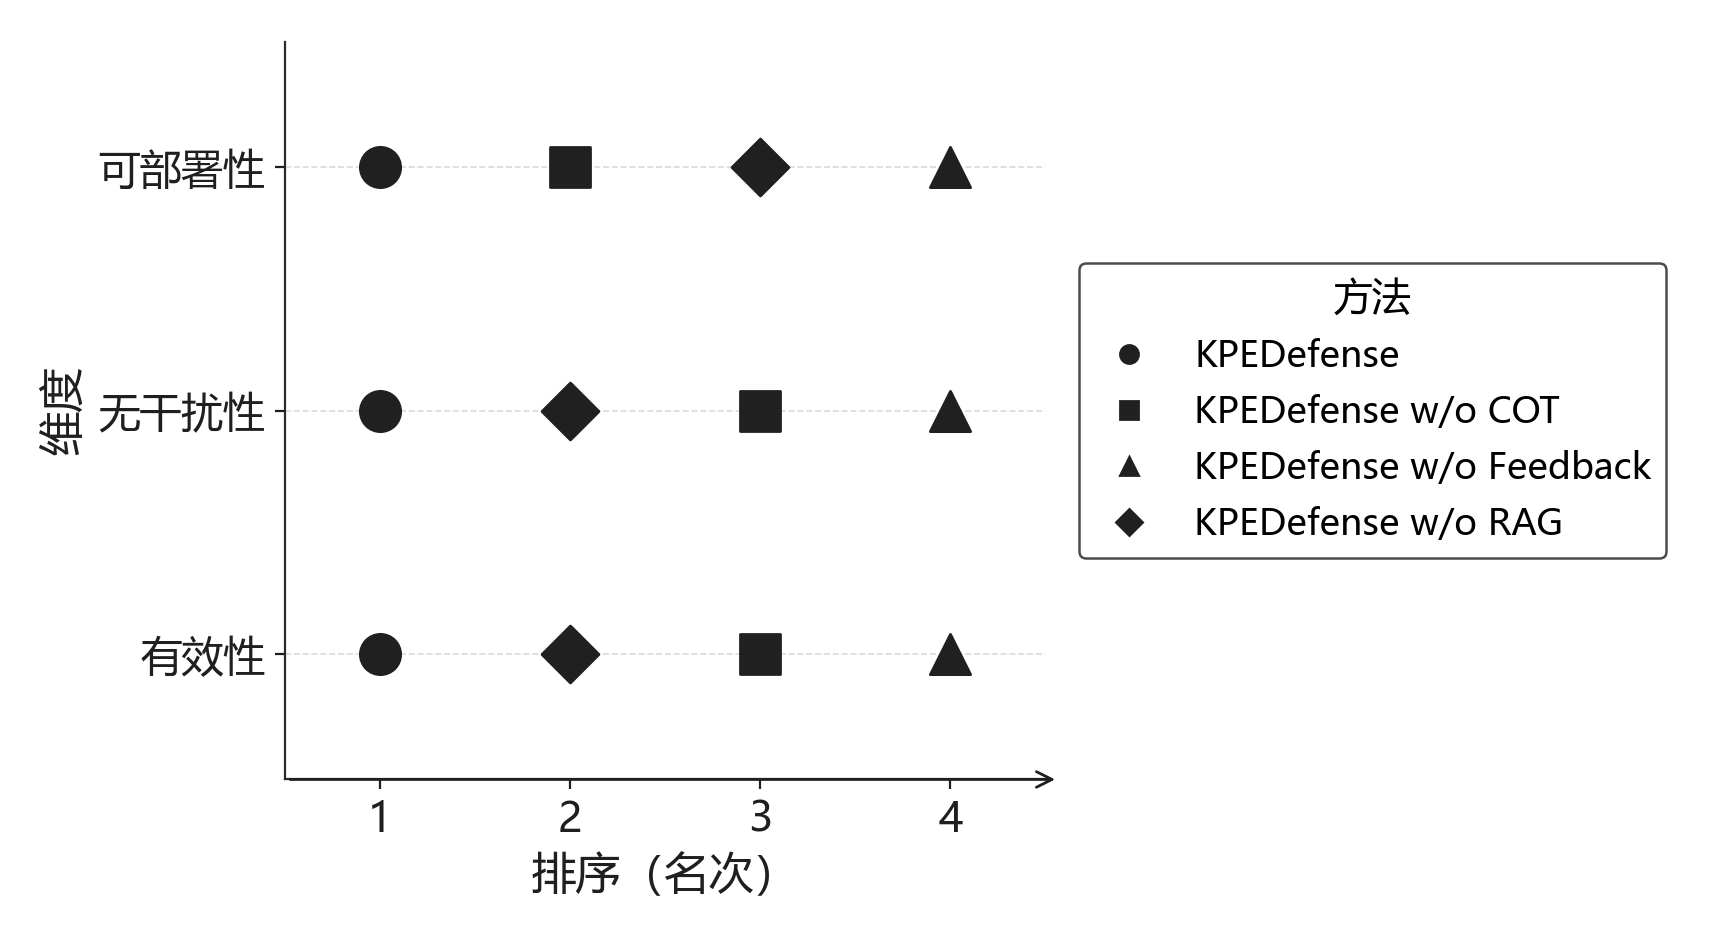
\includegraphics[width=0.85\textwidth]{images/output_rank_order/method_rank_order.png}}
	\caption{方法配置在三个维度上的排名对比。}\label{fig:method-ranking-overview}
\end{figure}

从图中可见，完整工作流 \texttt{all} 在三个维度上均排名第一（综合平均排名 $1.00$），显著优于任何消融配置。表\ref{tab:ablation-scores}给出了四种方法配置在三个维度上的详细得分。

\begin{table}[htb]
	\centering
	\bicaption{消融实验中各方法配置在三维度上的平均得分}{Average scores of method configurations across three dimensions in ablation study}
	\label{tab:ablation-scores}
	\setlength{\tabcolsep}{10pt}
	\renewcommand{\arraystretch}{1.3}
	\begin{tabularx}{0.75\linewidth}{>{\ttfamily\raggedright\arraybackslash}p{0.22\linewidth} *{3}{>{\centering\arraybackslash}X}}
	\toprule
	\textbf{方法配置} & \textbf{有效性($E$)} & \textbf{无干扰性($I$)} & \textbf{可部署性($D$)} \\
	\midrule
	all & 0.581 & 0.431 & 0.403 \\
	w/o rag & 0.476 & 0.370 & 0.321 \\
	w/o cot & 0.234 & 0.340 & 0.398 \\
	w/o feedback & 0.121 & 0.269 & 0.288 \\
	\bottomrule
	\end{tabularx}
\end{table}

\textbf{反馈迭代机制（Feedback）的核心作用：}移除反馈优化后，策略质量全面下降，三个维度得分分别为：$E=0.121$（下降79.2\%）、$I=0.269$（下降37.6\%）、$D=0.288$（下降28.5\%）。这表明迭代优化是工作流的核心环节，评审模型的多轮反馈能够持续引导生成模型修正缺陷，对有效性的提升尤为显著。

\textbf{检索增强（RAG）的知识支撑：}\texttt{w/o rag} 在有效性维度保持次优（$E=0.476$），显著优于 \texttt{w/o cot}（$E=0.234$）和 \texttt{w/o feedback}（$E=0.121$）。这说明检索增强模块为策略生成提供了关键的领域知识支撑，包括漏洞特征库、历史防控案例与Kubernetes安全最佳实践。在缺乏这些知识的情况下，生成模型更易产生不精确或不相关的策略。

\textbf{思维链推导（CoT）的双刃剑效应：}\texttt{w/o cot} 在有效性维度排名最低（$E=0.234$），但在可部署性维度接近完整工作流（$D=0.398$ vs. $D=0.403$）。这揭示了思维链推导的双重作用：虽能显著提升策略的漏洞覆盖率与防控逻辑严密性，但分阶段推导过程引入了更复杂的YAML配置结构与依赖关系，增加了部署门槛。在对安全性要求极高的场景下，应优先保留CoT模块；而在快速响应场景下，可适当简化推导过程以降低部署复杂度。

综上，三个模块的协同作用为策略生成提供了一致性增益，其重要性排序为：\textbf{Feedback > RAG > CoT}。完整工作流在三个维度上分别达到0.581（有效性）、0.431（无干扰性）与0.403（可部署性）的最优表现。在实际部署中，若资源受限需简化工作流，建议优先保留反馈迭代机制与检索增强模块。

\subsection{工作流跨模型稳健性验证}

为验证上述消融实验结论是否对不同生成模型稳健，本小节分析完整工作流相对消融配置的优势在不同模型条件下的一致性。

图\ref{fig:effectiveness-profile-avg} 给出不同生成模型在有效性维度的平均排名。图\ref{fig:effectiveness-generator-by-method} 与图\ref{fig:effectiveness-generator-grouped} 从生成模型视角展开方法配置贡献结构。

\begin{figure}[!ht]
	\centering
	{\setlength{\abovecaptionskip}{2pt}%
	 \setlength{\belowcaptionskip}{0pt}%
	 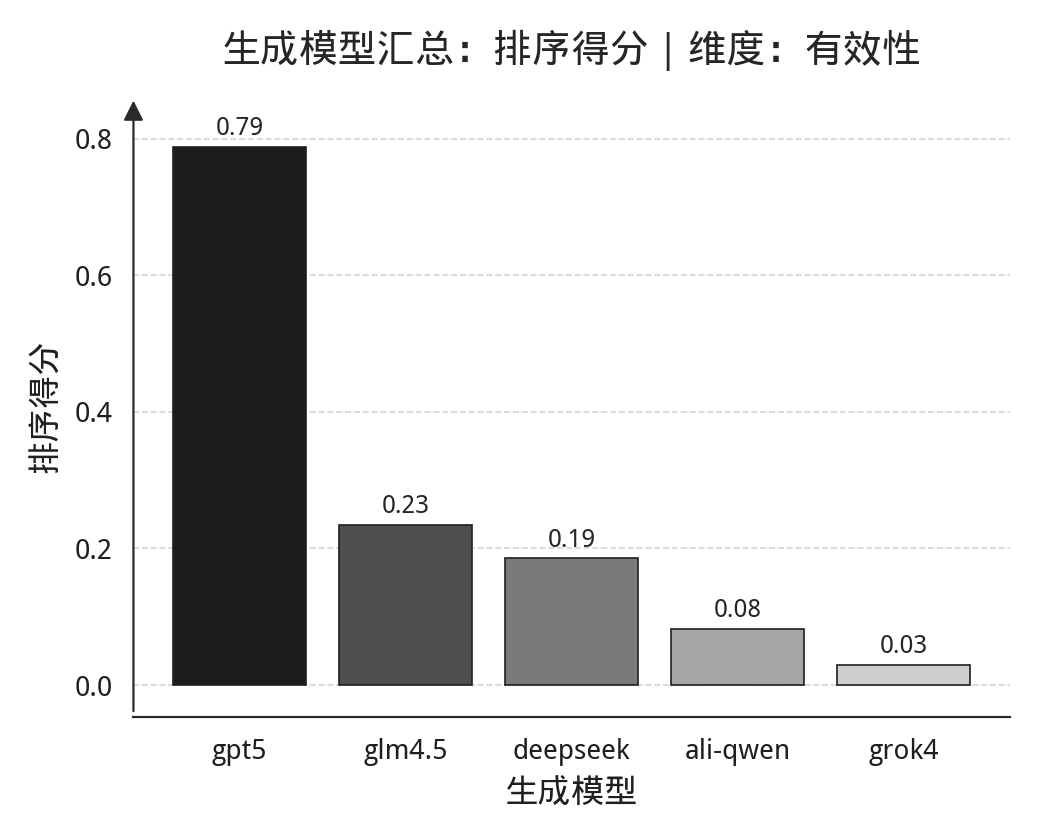
\includegraphics[width=0.85\textwidth]{images/plots/有效性/summary/single_dim_profile_avg_有效性.png}}
	\caption{有效性维度下，不同生成模型的平均排名式评分结果（跨评审者汇总）。}\label{fig:effectiveness-profile-avg}
\end{figure}

\begin{figure}[!ht]
	\centering
	{\setlength{\abovecaptionskip}{2pt}%
	 \setlength{\belowcaptionskip}{0pt}%
	 \subfloat[\texttt{Qwen3}\label{fig:effectiveness-generator-by-method-qwen3}]{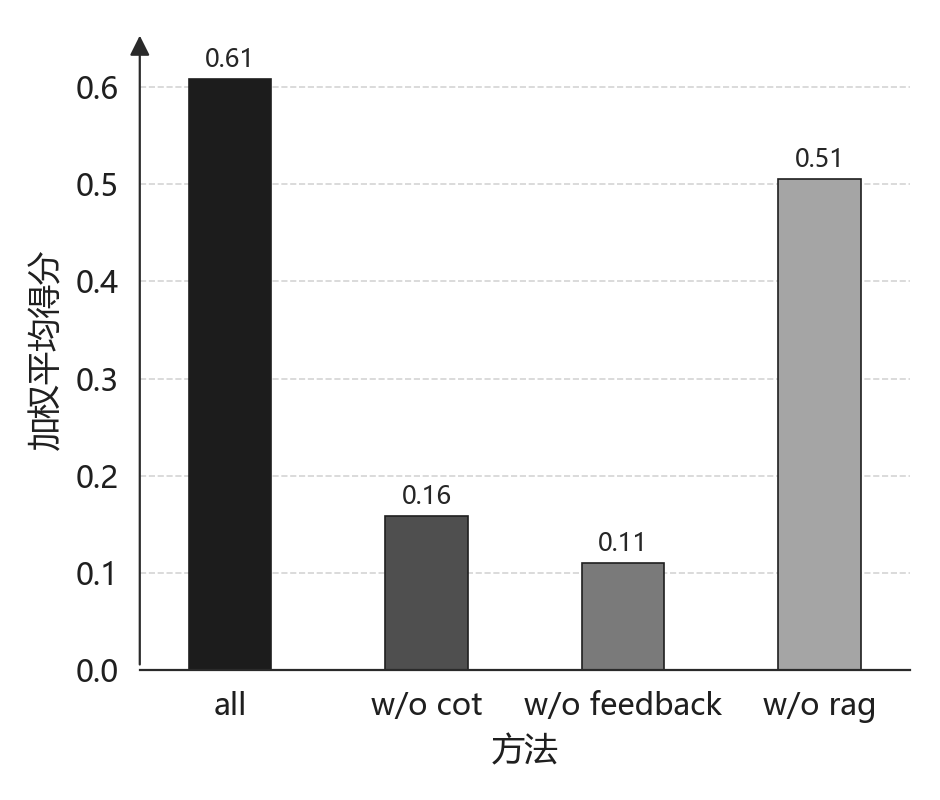
\includegraphics[width=0.32\textwidth]{images/plots/有效性/generator/ali-qwen/generator_bar_by_method_ali-qwen_有效性.png}}\hfill
	 \subfloat[\texttt{DeepSeek}\label{fig:effectiveness-generator-by-method-deepseek}]{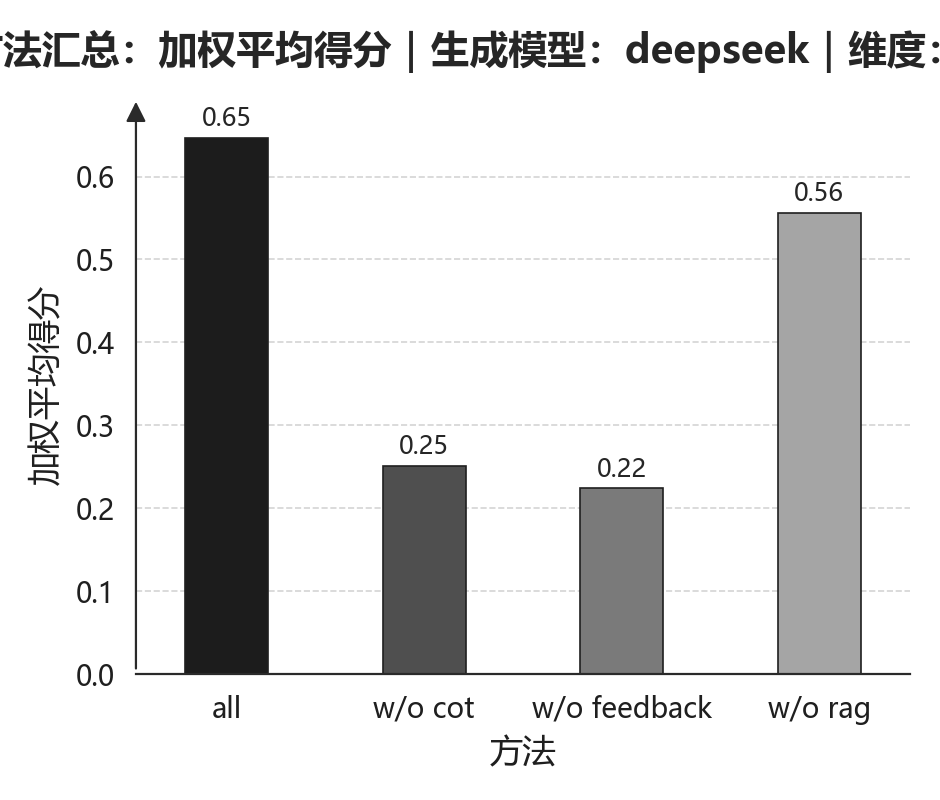
\includegraphics[width=0.32\textwidth]{images/plots/有效性/generator/deepseek/generator_bar_by_method_deepseek_有效性.png}}\hfill
	 \subfloat[\texttt{GPT-5}\label{fig:effectiveness-generator-by-method-gpt5}]{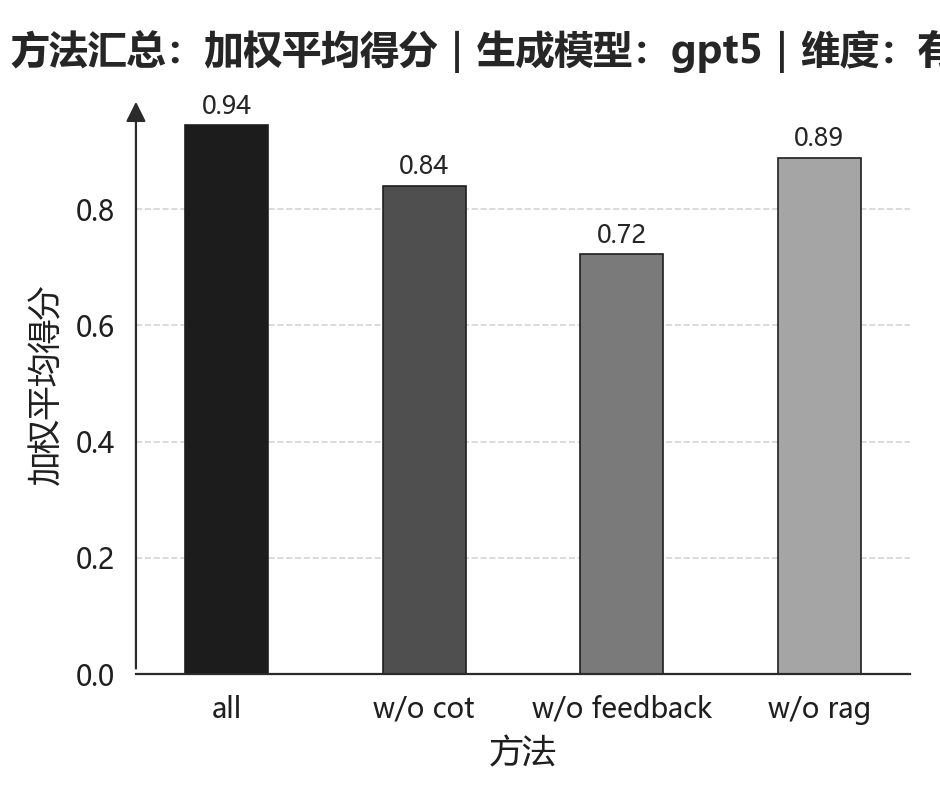
\includegraphics[width=0.32\textwidth]{images/plots/有效性/generator/gpt5/generator_bar_by_method_gpt5_有效性.png}}\\
	 \subfloat[\texttt{Grok}\label{fig:effectiveness-generator-by-method-grok}]{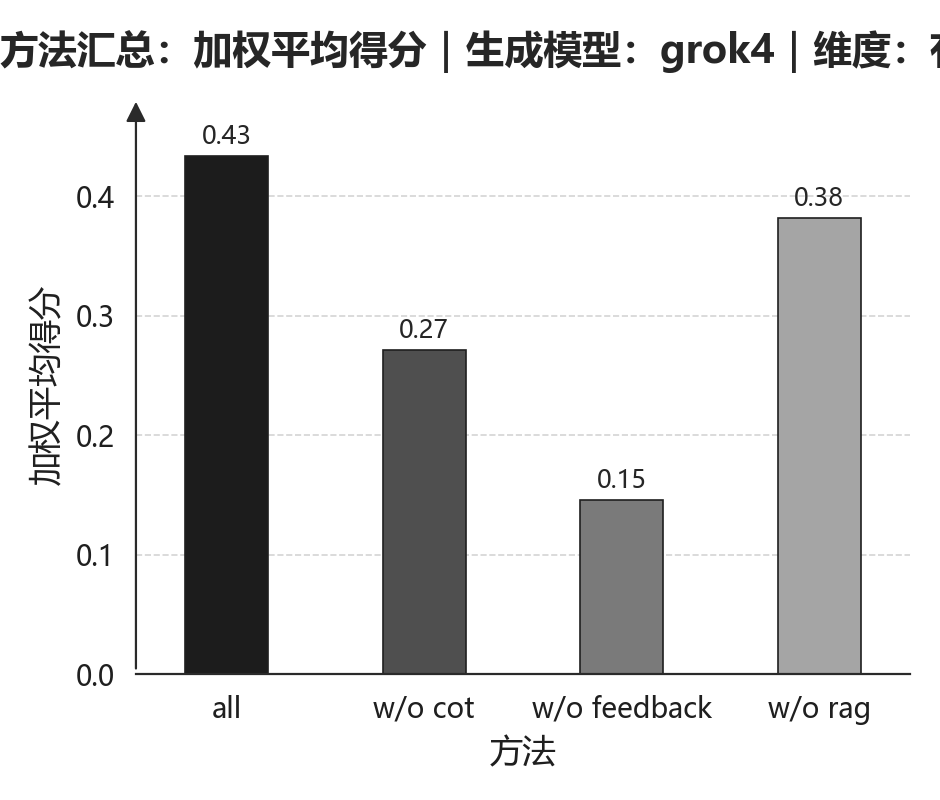
\includegraphics[width=0.32\textwidth]{images/plots/有效性/generator/grok4/generator_bar_by_method_grok4_有效性.png}}\hfill
	 \subfloat[\texttt{GLM-4.6}\label{fig:effectiveness-generator-by-method-glm46}]{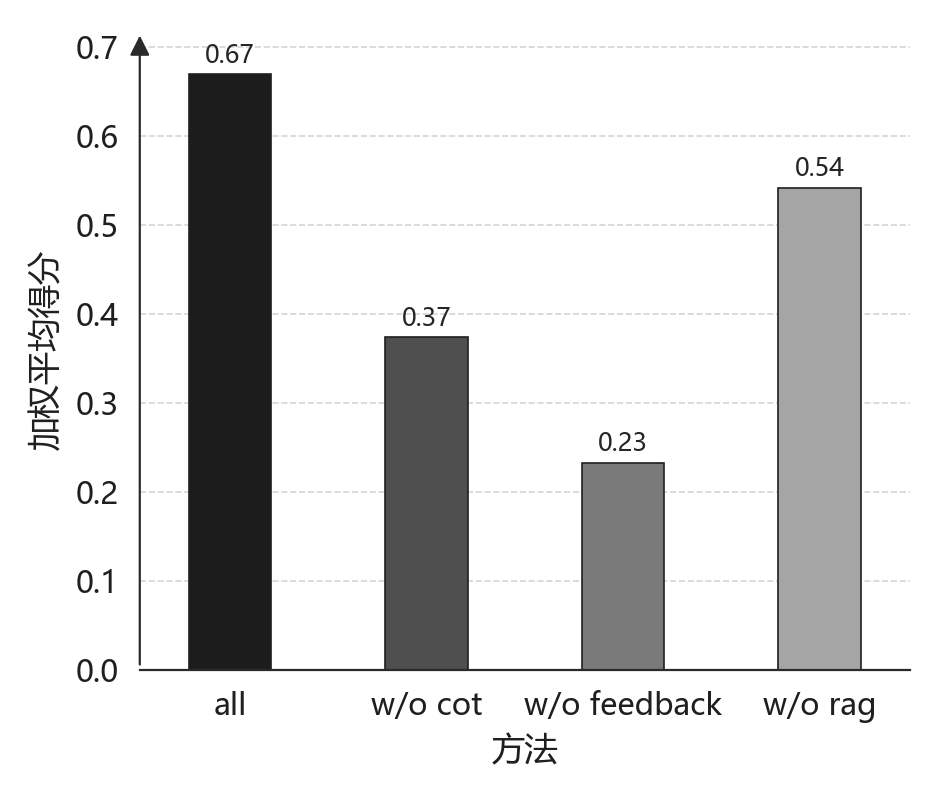
\includegraphics[width=0.32\textwidth]{images/plots/有效性/generator/glm4.5/generator_bar_by_method_glm4.5_有效性.png}}}
	\caption{有效性维度下，不同生成模型的工作流贡献结构对照（3+2 网格）。}\label{fig:effectiveness-generator-by-method}
\end{figure}

\begin{figure}[!ht]
	\centering
	{\setlength{\abovecaptionskip}{2pt}%
	 \setlength{\belowcaptionskip}{0pt}%
	 \subfloat[\texttt{Qwen3}\label{fig:effectiveness-generator-grouped-qwen3}]{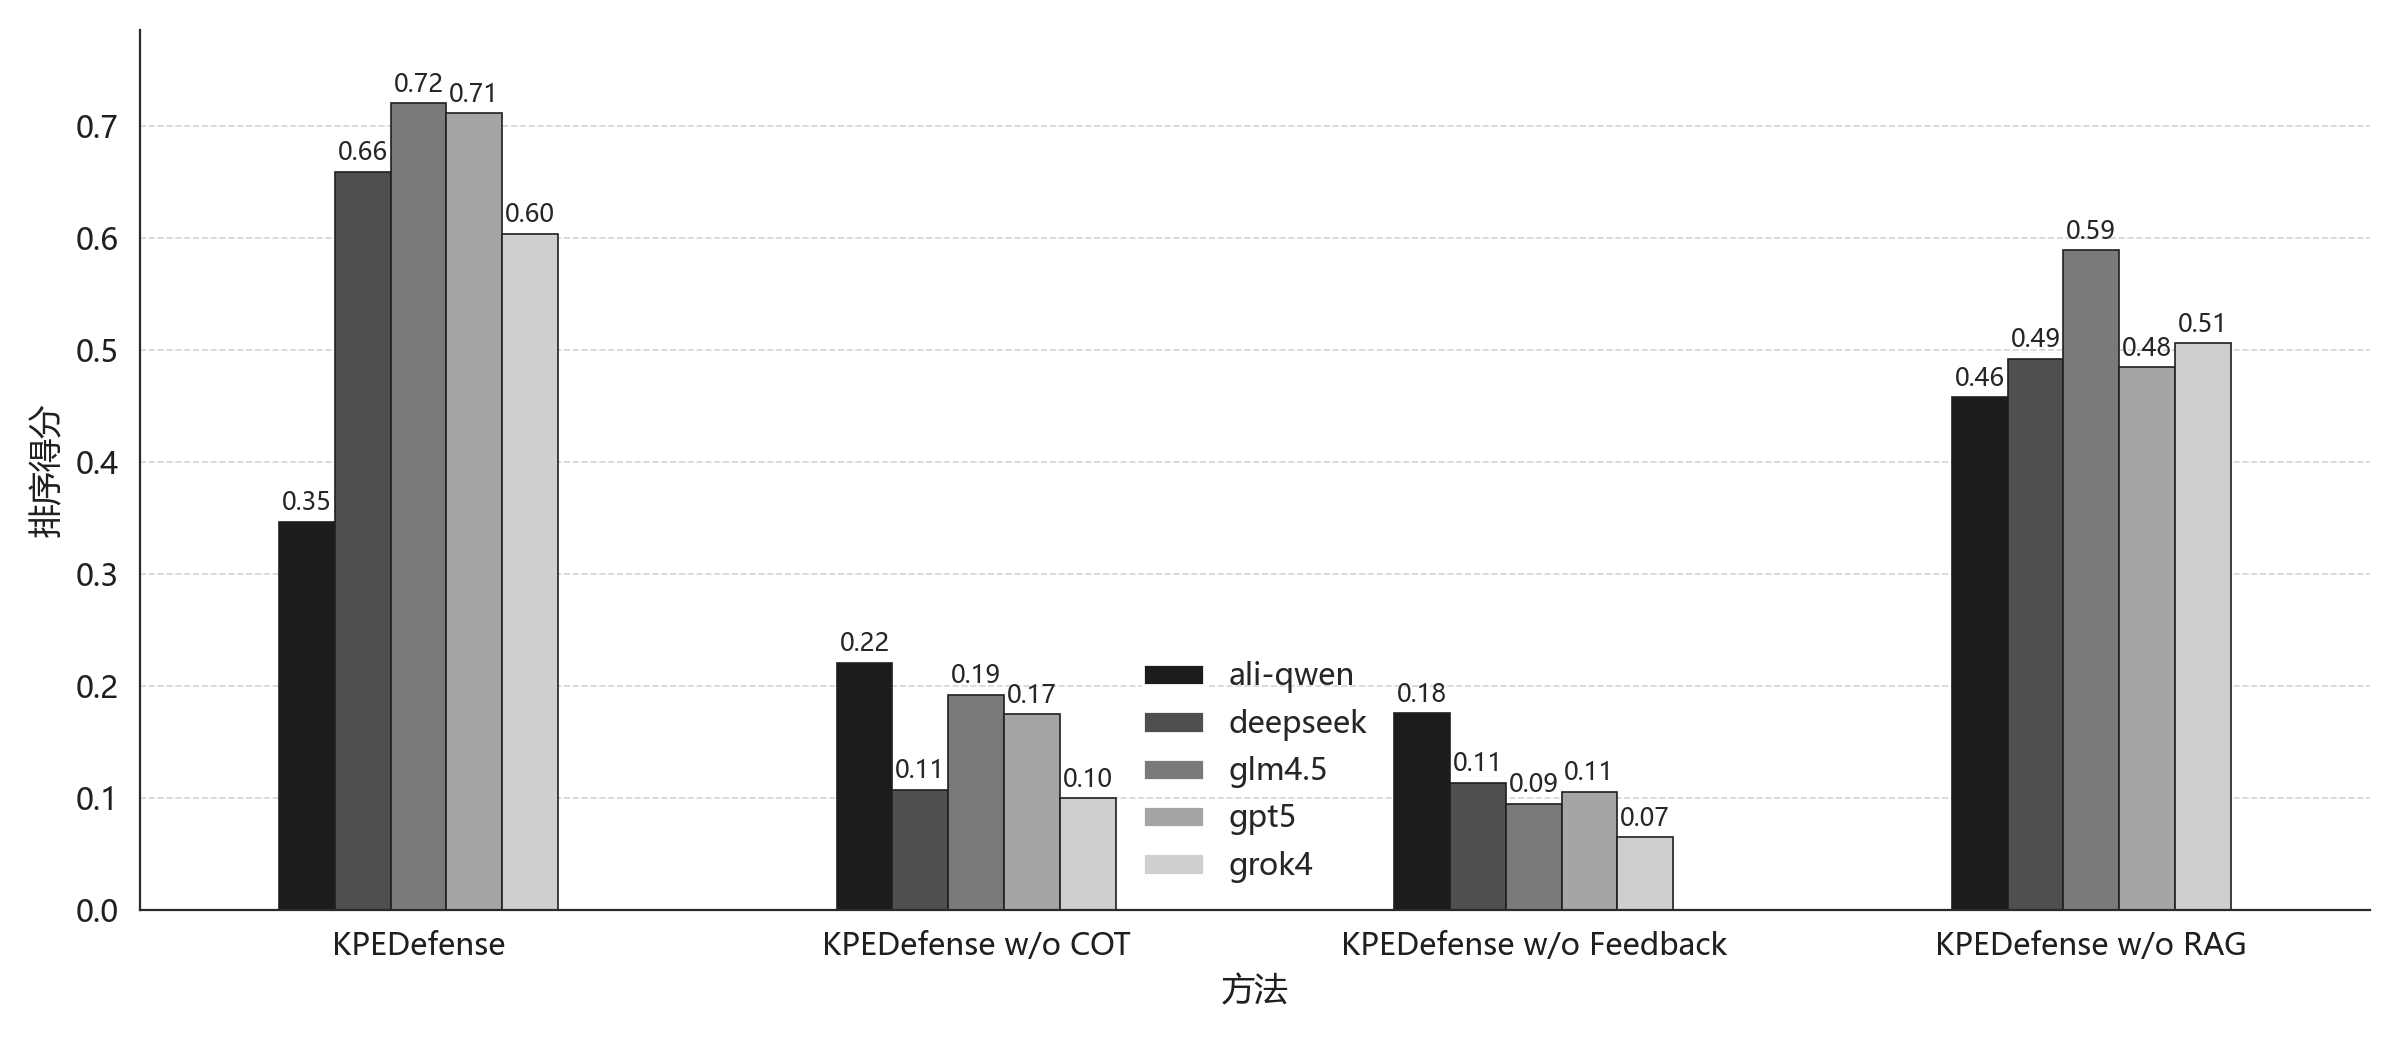
\includegraphics[width=0.32\textwidth]{images/plots/有效性/generator/ali-qwen/grouped_bar_ali-qwen_有效性.png}}\hfill
	 \subfloat[\texttt{DeepSeek}\label{fig:effectiveness-generator-grouped-deepseek}]{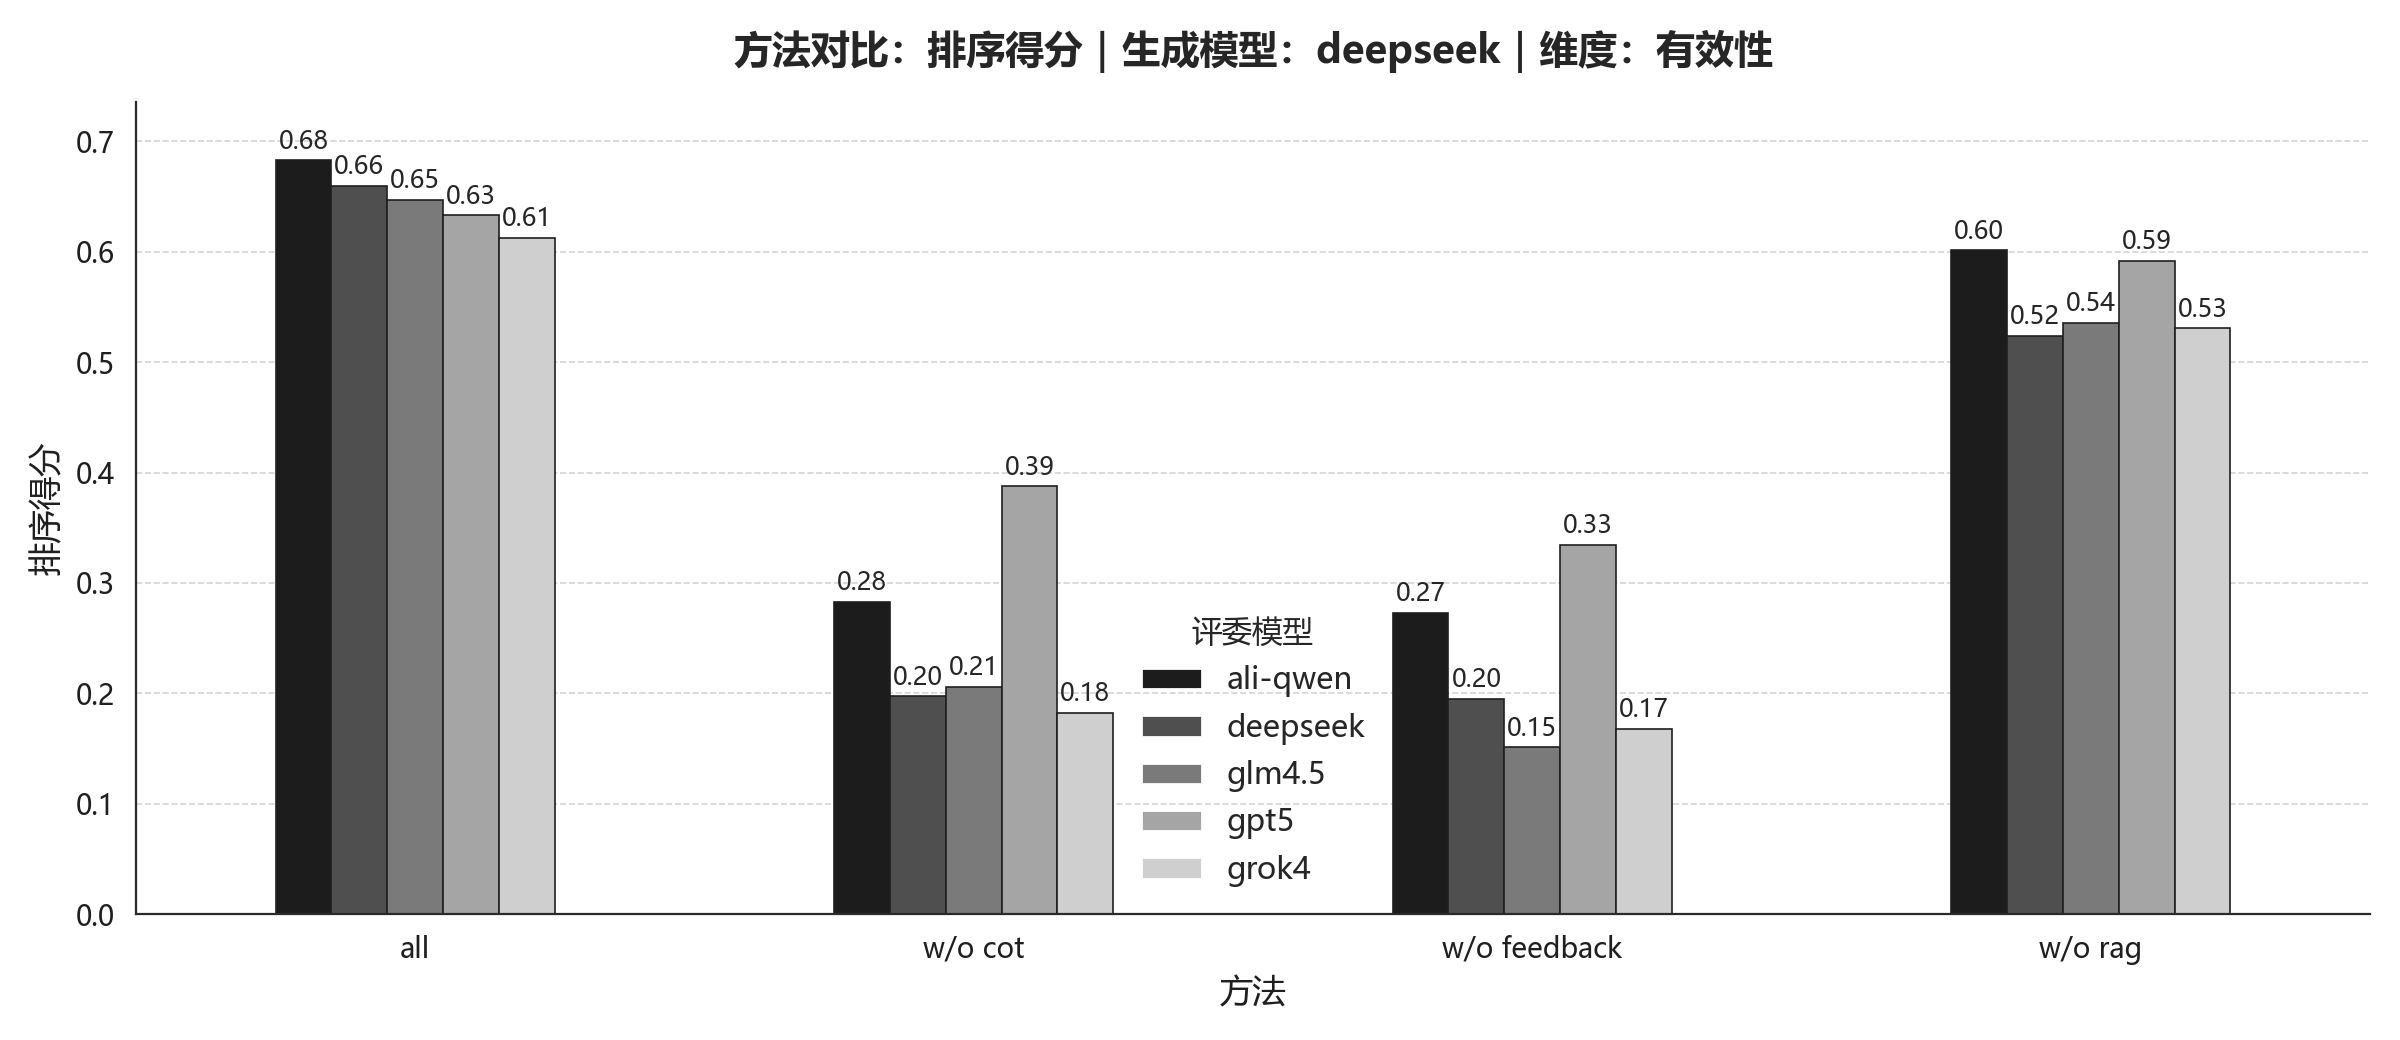
\includegraphics[width=0.32\textwidth]{images/plots/有效性/generator/deepseek/grouped_bar_deepseek_有效性.png}}\hfill
	 \subfloat[\texttt{GPT-5}\label{fig:effectiveness-generator-grouped-gpt5}]{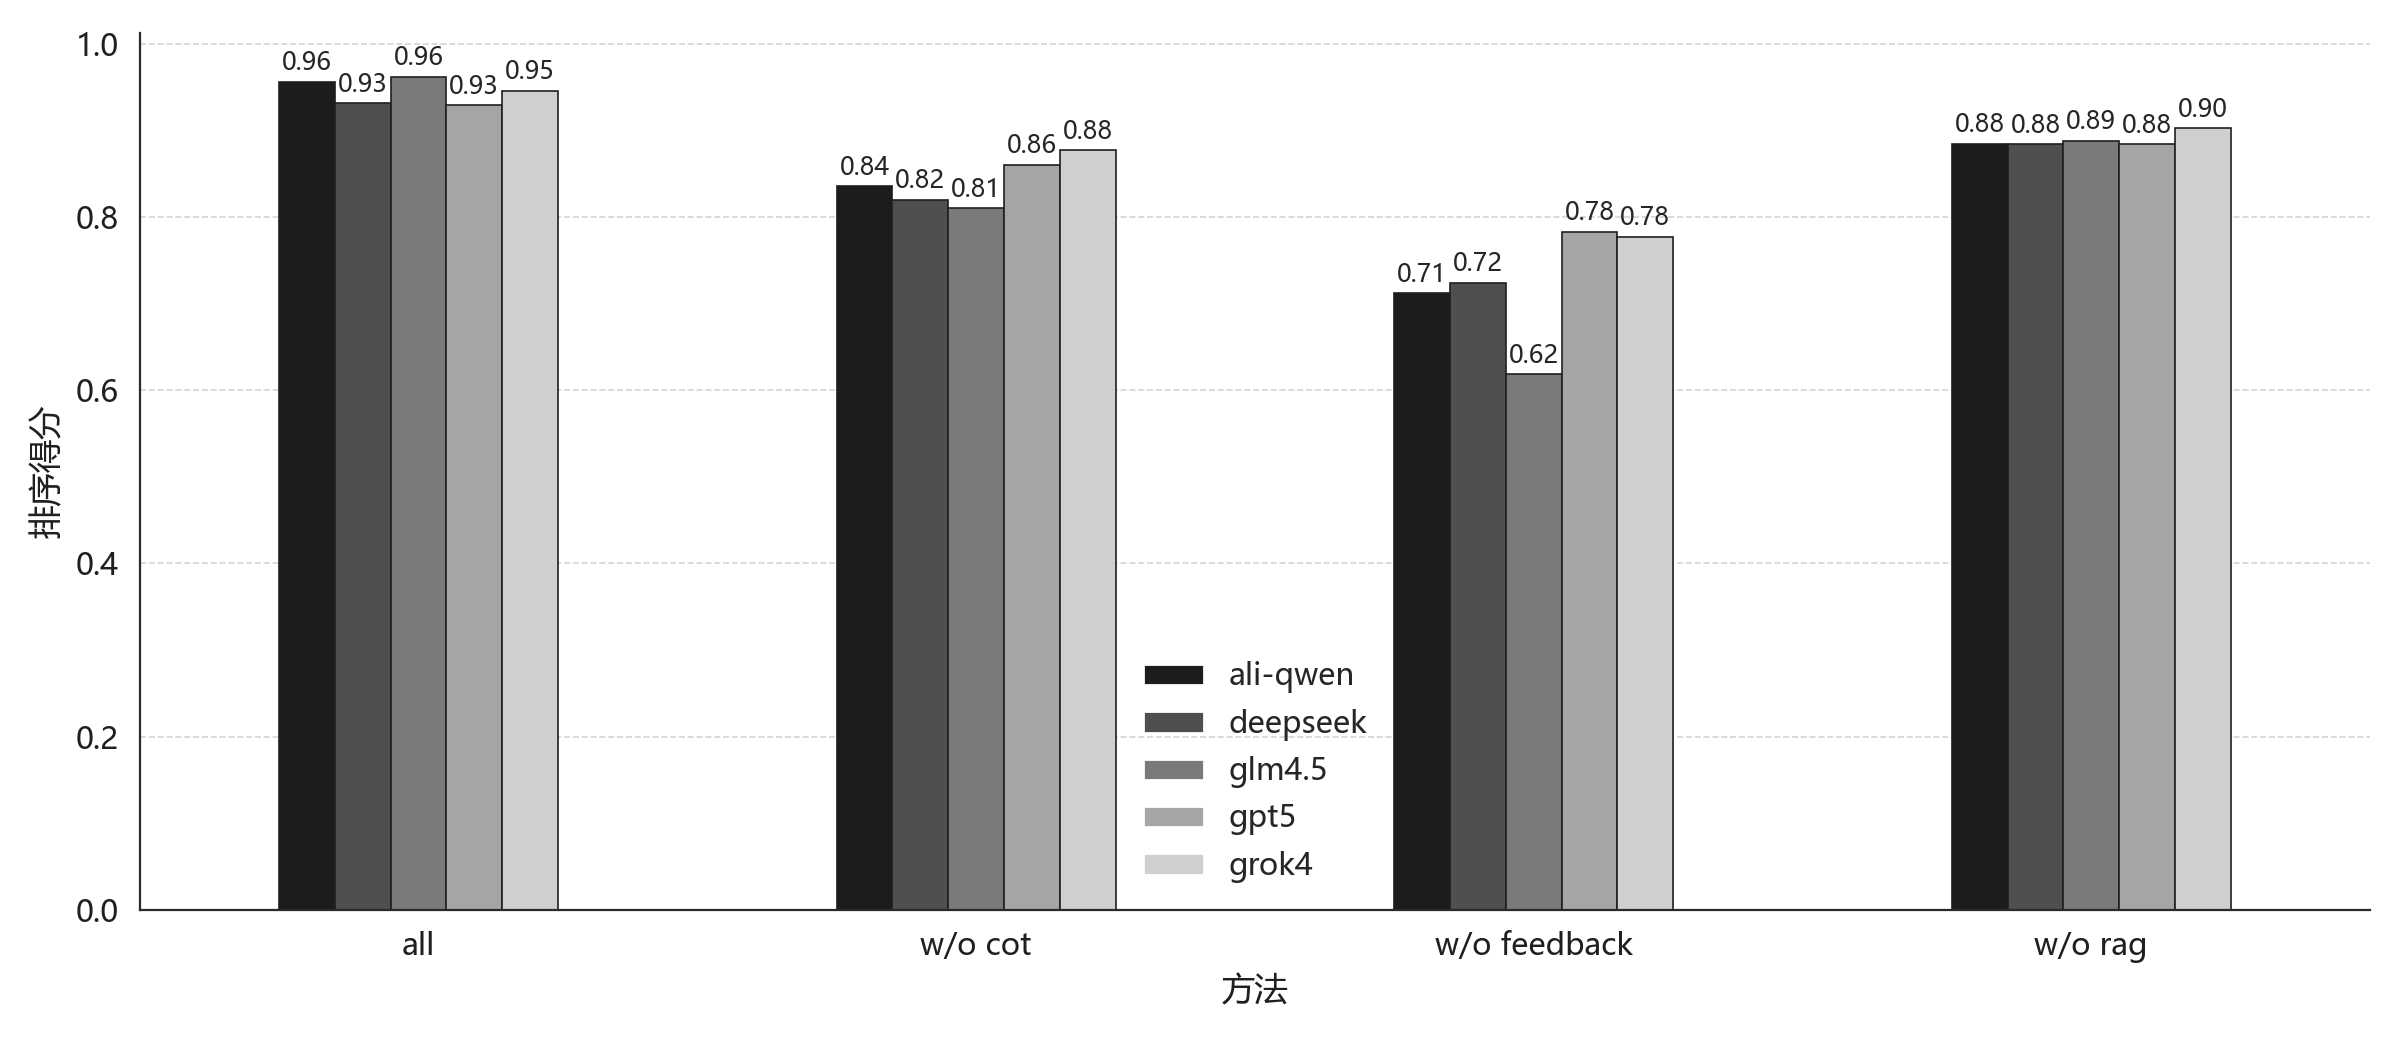
\includegraphics[width=0.32\textwidth]{images/plots/有效性/generator/gpt5/grouped_bar_gpt5_有效性.png}}\\
	 \subfloat[\texttt{Grok}\label{fig:effectiveness-generator-grouped-grok}]{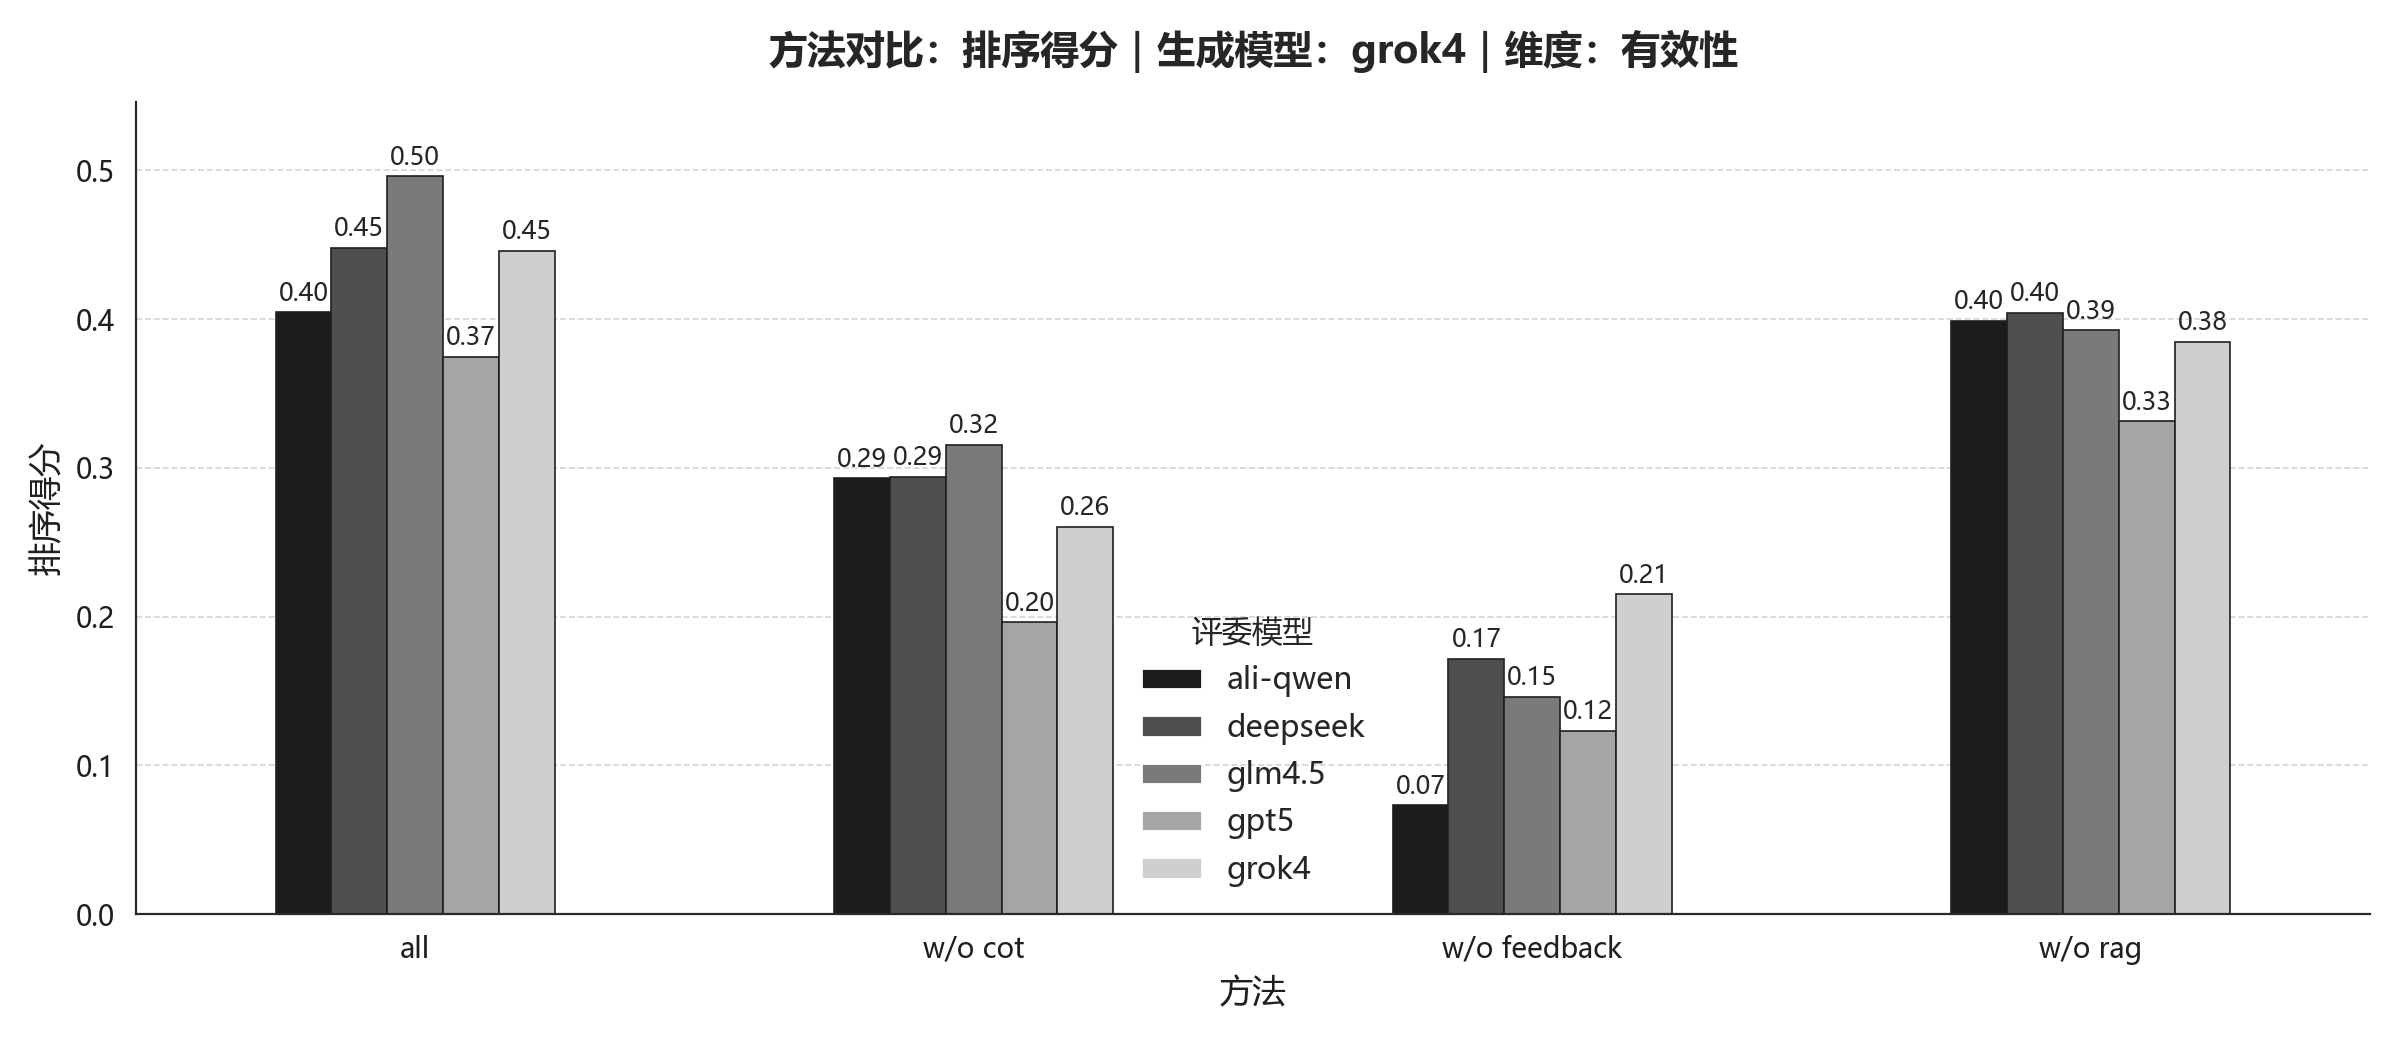
\includegraphics[width=0.32\textwidth]{images/plots/有效性/generator/grok4/grouped_bar_grok4_有效性.png}}\hfill
	 \subfloat[\texttt{GLM-4.6}\label{fig:effectiveness-generator-grouped-glm46}]{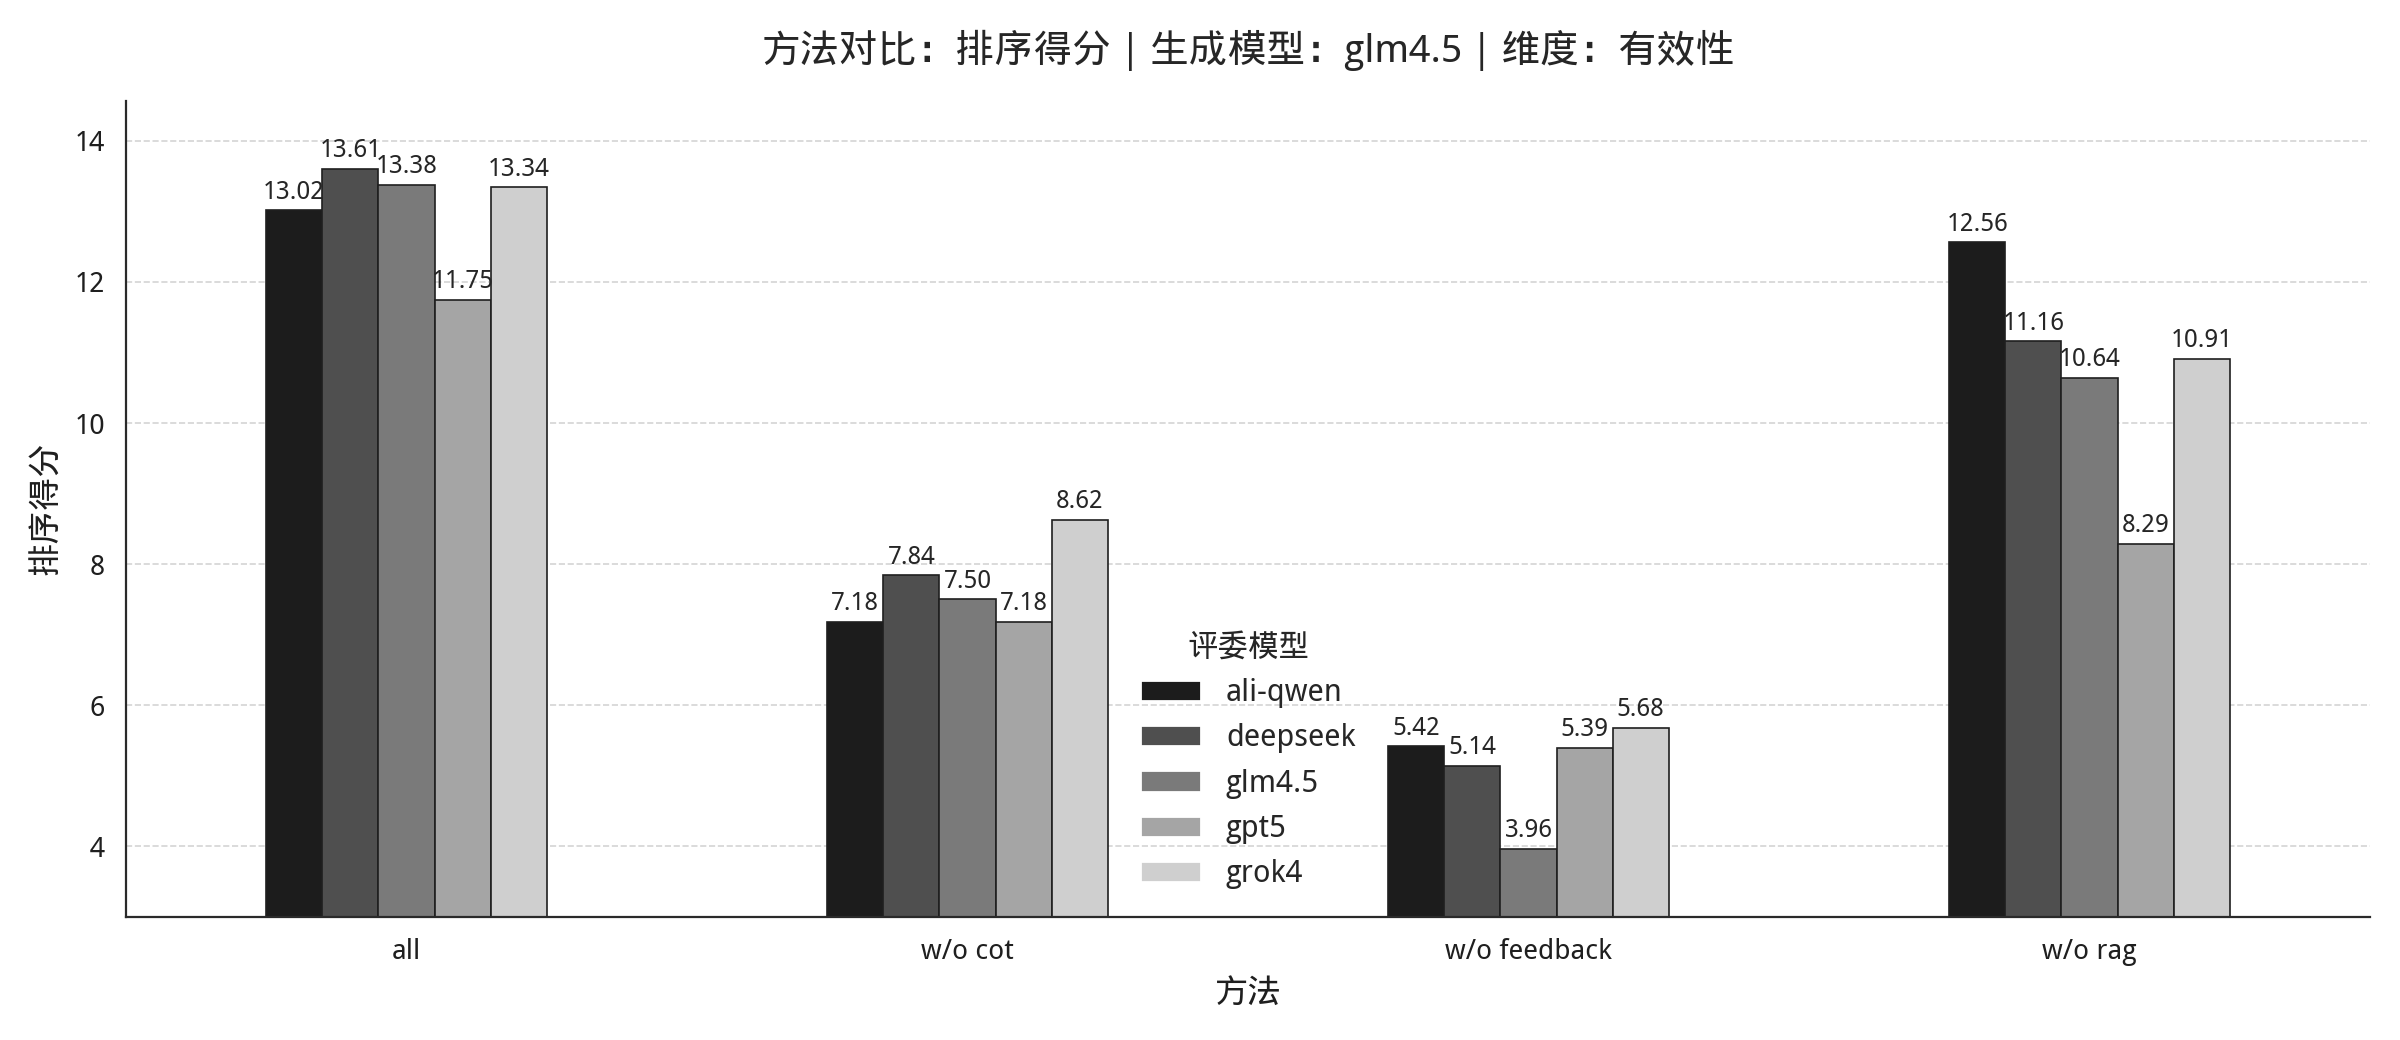
\includegraphics[width=0.32\textwidth]{images/plots/有效性/generator/glm4.5/grouped_bar_glm4.5_有效性.png}}}
	\caption{有效性维度下，不同生成模型的分组条形图对照（3+2 网格）。}\label{fig:effectiveness-generator-grouped}
\end{figure}

从图中可见，完整工作流（\texttt{all}）在五个生成模型条件下均保持最优或次优排名，验证了消融实验结论的跨模型稳健性。不同生成模型对各模块的依赖程度存在差异：GPT-5 与 GLM-4.5 对反馈迭代的依赖性更强，移除反馈后排名下降明显；而 DeepSeek 与 Qwen3 对检索增强的响应更为敏感，说明不同模型在知识库支撑与迭代优化上的需求存在差异。

\section{RQ2：生成模型能力评估}

本节从策略生成质量与输出稳定性两个维度评估五个生成模型的能力特征，识别不同模型在三维质量指标上的取舍倾向与适用场景。

\subsection{三维质量指标的能力分化}

图\ref{fig:generator-ranking-overview}展示了五个生成模型在有效性（$E$）、无干扰性（$I$）与可部署性（$D$）三个维度上的排名分布。

\begin{figure}[!ht]
	\centering
	{\setlength{\abovecaptionskip}{2pt}%
	 \setlength{\belowcaptionskip}{0pt}%
	 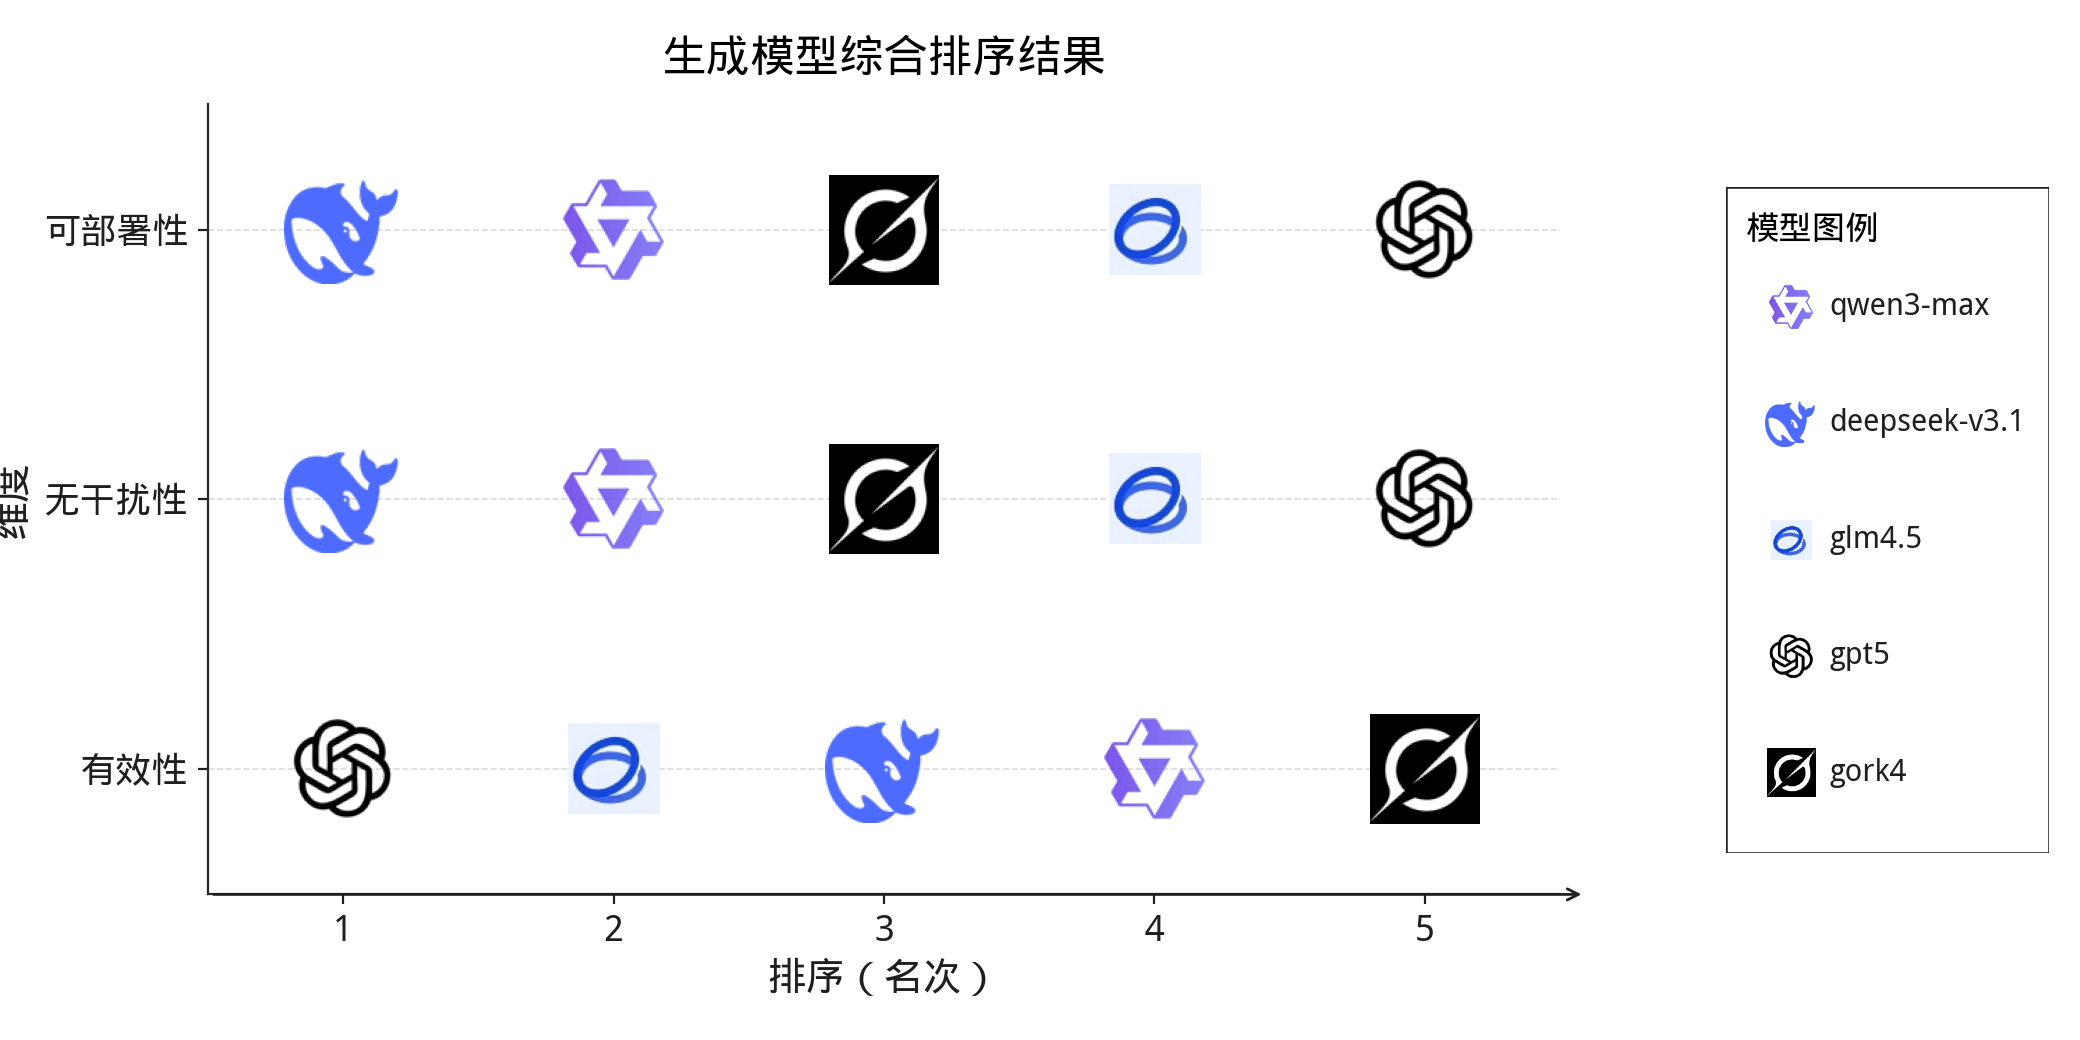
\includegraphics[width=0.85\textwidth]{images/output_rank_order/profile_rank_order.png}}
	\caption{生成模型在三个维度上的排名对比。}\label{fig:generator-ranking-overview}
\end{figure}

表\ref{tab:generator-scores}给出了五个生成模型在三个维度上的详细得分，揭示了显著的能力分化现象。

\begin{table}[htb]
	\centering
	\bicaption{生成模型在三维度上的平均得分}{Average scores of generation models across three dimensions}
	\label{tab:generator-scores}
	\setlength{\tabcolsep}{8pt}
	\renewcommand{\arraystretch}{1.3}
	\begin{tabularx}{0.85\linewidth}{>{\ttfamily\raggedright\arraybackslash}p{0.20\linewidth} *{3}{>{\centering\arraybackslash}X} >{\centering\arraybackslash}p{0.15\linewidth}}
	\toprule
	\textbf{生成模型} & \textbf{有效性($E$)} & \textbf{无干扰性($I$)} & \textbf{可部署性($D$)} & \textbf{综合评价} \\
	\midrule
	GPT-5 & \textbf{0.814} & 0.175 & 0.000 & 安全优先型 \\
	GLM-4.5 & 0.327 & 0.324 & 0.336 & 中等均衡型 \\
	DeepSeek & 0.284 & \textbf{0.497} & \textbf{0.605} & 部署优先型 \\
	Qwen3-Max & 0.193 & 0.425 & 0.477 & 稳定通用型 \\
	Grok4 & 0.147 & 0.342 & 0.346 & 轻量快速型 \\
	\bottomrule
	\end{tabularx}
\end{table}

\textbf{DeepSeek 3.1：部署优先型优选方案。}\texttt{DeepSeek 3.1} 在可部署性与无干扰性维度表现卓越（$D=0.605$，$I=0.497$），均位列首位，但在有效性维度处于中游（$E=0.284$）。这表明 DeepSeek 擅长生成简洁、低侵入性的策略，能够有效平衡漏洞防控与实际部署约束，规避过度复杂的配置设计。该特性使其成为对部署速度与业务连续性敏感的生产环境的首选方案，尤其适用于需要快速响应新披露漏洞的场景。

\textbf{GPT-5：安全优先型方案。}\texttt{GPT-5} 呈现极端的维度分化特征：在有效性维度遥遥领先（$E=0.814$），但在无干扰性与可部署性维度排名垫底（$I=0.175$，$D=0.000$）。这一分化现象揭示 GPT-5 在生成策略时极度注重漏洞防控的彻底性，倾向于采用严格的RBAC限制、网络隔离与准入控制措施，不惜牺牲策略的简洁性与部署便利性。该模型适用于对安全性要求极高且可容忍高部署成本的关键基础设施场景，如金融、政务等领域的Kubernetes集群防护。

\textbf{Qwen3-Max：稳定通用型方案。}\texttt{Qwen3-Max} 在三维度上保持中上水平（$E=0.193$，$I=0.425$，$D=0.477$），无明显短板，呈现较为均衡的能力分布。虽未在任何单一维度上拔尖，但其稳定性使其可作为通用型选择，适用于对三个维度均有一定要求且需要平衡多目标的场景。

\textbf{GLM-4.5：中等均衡型方案。}\texttt{GLM-4.5} 在三个维度上得分接近（$E=0.327$，$I=0.324$，$D=0.336$），表现出良好的均衡性，但整体水平处于中游。其维度分化程度较小，适合作为多模型组合策略中的补充选择。

\textbf{Grok4：轻量快速型方案。}\texttt{Grok4} 在有效性维度排名最低（$E=0.147$），但在无干扰性与可部署性维度保持中游水平（$I=0.342$，$D=0.346$）。这表明 Grok4 倾向于生成简单、轻量级的策略，虽然防控效果有限，但部署门槛低、响应速度快，适用于低风险漏洞的临时防控或作为快速应急响应方案。

\subsection{输出稳定性评估}

为评估不同生成模型在策略生成过程中的输出稳定性，本文统计了各模型在生成阶段触发重试的次数。重试机制主要针对三类失败情形：结构化输出的 JSON 格式错误（通常因字段缺失、括号不匹配或编码问题）、生成内容的语法错误（包括 YAML 语法错误、逻辑矛盾或不可解析的配置片段），以及内容违规（触发模型供应商的安全策略或内容审核机制）。为便于跨模型对比，本文将计数按固定分母 504 归一化为失误率。表\ref{tab:model-retry-stats} 给出五个生成模型的失误率统计（=计数/504）。

\begin{table}[htb]
	\centering
	\bicaption{生成模型在策略生成过程中的重试失误率（\%）统计（=计数/504）}{Failure rates (\%) of retry-triggering errors during strategy generation across LLMs (=count/504)}
    \label{tab:model-retry-stats}
	\setlength{\tabcolsep}{8pt}
	\renewcommand{\arraystretch}{1.2}
	\small
	\begin{tabularx}{0.95\linewidth}{>{\raggedright\arraybackslash}p{2.6cm} *{5}{>{\centering\arraybackslash}X}}
    \toprule
	\textbf{错误类型} & \makecell{\textbf{DeepSeek}\\\textbf{3.1}} & \makecell{\textbf{GLM}\\\textbf{-4.5}} & \makecell{\textbf{GPT}\\\textbf{-5}} & \makecell{\textbf{Grok}\\\textbf{4}} & \makecell{\textbf{Qwen}\\\textbf{3}} \\
    \midrule
	JSON 格式错误 & 0.99\% & 4.56\% & 0.00\% & 0.99\% & 2.58\% \\
	语法错误 & 0.60\% & 1.98\% & 0.00\% & 0.00\% & 0.99\% \\
	内容违规 & 0.00\% & 1.98\% & 0.00\% & 0.00\% & 0.00\% \\
	\addlinespace[0.25em]\midrule
	\textbf{合计} & \textbf{1.59\%} & \textbf{8.53\%} & \textbf{0.00\%} & \textbf{0.99\%} & \textbf{3.57\%} \\
    \bottomrule
	\end{tabularx}
\end{table}

整体上，GPT-5 在三类错误上均无重试记录，表现出较高的生成鲁棒性；Grok 和 DeepSeek 的失误率较低，输出稳定性良好；Qwen3 与 GLM-4.5 的失误率相对较高，尤其在 JSON 格式错误上，GLM-4.5 的失误率为 4.56\%（=23/504），反映其在结构化输出约束下的遵循能力有待提升。语法错误维度上，GLM-4.5 同样表现出明显劣势（1.98\%=10/504），而其余模型均不超过 0.99\%（=5/504）。值得注意的是，GLM-4.5 是唯一触发内容违规的模型（1.98\%=10/504），可能与其内容审核策略对高危漏洞描述中的安全关键词过度敏感相关。

该统计为模型选型与多智能体协同策略提供了量化参考：在资源受限或对输出稳定性敏感的场景下，优先选用 GPT-5、Grok 或 DeepSeek；而对于需要多样性候选集的场景，可将 Qwen3 与 GLM-4.5 纳入候选池，但需配置更宽松的重试预算与后处理容错机制。

\subsection{生成模型能力评估小结}

五个生成模型在三维质量指标上表征出明显的能力分化与取舍倾向：DeepSeek 的部署优势（$D=0.605$）使其成为生产环境首选；GPT-5 的安全优势（$E=0.814$）适用于高安全要求场景；Grok4 可作为快速响应的轻量级方案（$D=0.346$，响应时间最短）。

进一步分析各生成模型的最佳方法配置（表\ref{tab:best-method-per-generator}）发现，所有模型在完整工作流（\texttt{all}）配置下均达到最优或次优表现，验证了RQ1消融实验结论的跨模型稳健性。值得注意的是，DeepSeek 在 \texttt{w/o cot} 配置下的可部署性得分达到0.749，超过完整工作流的0.678，进一步证实了思维链推导在提升防控效果的同时会增加部署复杂度的双刃剑效应。

\begin{table}[htb]
	\centering
	\bicaption{各生成模型的最佳方法配置与得分}{Best method configuration and score for each generation model}
	\label{tab:best-method-per-generator}
	\setlength{\tabcolsep}{8pt}
	\renewcommand{\arraystretch}{1.3}
	\begin{tabularx}{0.90\linewidth}{>{\ttfamily\raggedright\arraybackslash}p{0.18\linewidth} >{\centering\arraybackslash}X >{\centering\arraybackslash}X >{\centering\arraybackslash}X}
	\toprule
	\textbf{生成模型} & \textbf{有效性最佳} & \textbf{无干扰性最佳} & \textbf{可部署性最佳} \\
	\midrule
	GPT-5 & all (0.945) & w/o cot (0.369) & w/o cot (0.256) \\
	GLM-4.5 & all (0.670) & all (0.522) & all (0.504) \\
	DeepSeek & all (0.647) & w/o rag (0.634) & w/o cot (0.749) \\
	Qwen3-Max & all (0.609) & all (0.629) & all (0.656) \\
	Grok4 & all (0.434) & all (0.589) & all (0.597) \\
	\bottomrule
	\end{tabularx}
\end{table}

在输出稳定性上，GPT-5、Grok 与 DeepSeek 表现优异（失误率分别为0.00\%、0.99\%与1.59\%），而 GLM-4.5 与 Qwen3 需额外关注结构化输出约束（失误率分别为8.53\%与3.57\%）。这些实证发现为后续基于维度加权的多智能体策略组合提供了依据：在实际部署中，可依据具体漏洞的风险等级与业务约束动态选择或组合不同生成模型——对于高危漏洞优先选择GPT-5或GLM-4.5以提升防控彻底性，对于需快速部署的场景优先选择DeepSeek或Qwen3-Max以降低实施难度。

\section{RQ3：评审模型一致性评估}

为验证排名式评价的可信度，本节分析不同评审模型在单一维度与跨维度场景下的一致性，以支撑前述跨评审聚合统计与反馈闭环（RQ1--RQ2）。若不同评审者（评审模型）对候选项优劣的判断高度一致，则聚合后的排序结果更稳定、更可解释；反之，若一致性较弱，则需要警惕"评审者选择敏感性"，并进一步细化评价准则。

\subsection{跨维度的评审差异}

图\ref{fig:single-dim-by-judge-3d} 展示不同评审模型下的单维度排名式结果，反映评审模型之间的尺度差异与偏好结构。图\ref{fig:single-dim-profile-avg} 则从生成模型角度给出三维度总体表现，用于观察生成模型在 $E/I/D$ 上的系统性取舍。

\begin{figure}[!ht]
	\centering
	{\setlength{\abovecaptionskip}{2pt}%
	 \setlength{\belowcaptionskip}{0pt}%
	 \subfloat[可部署性\label{fig:single-dim-deployability}]{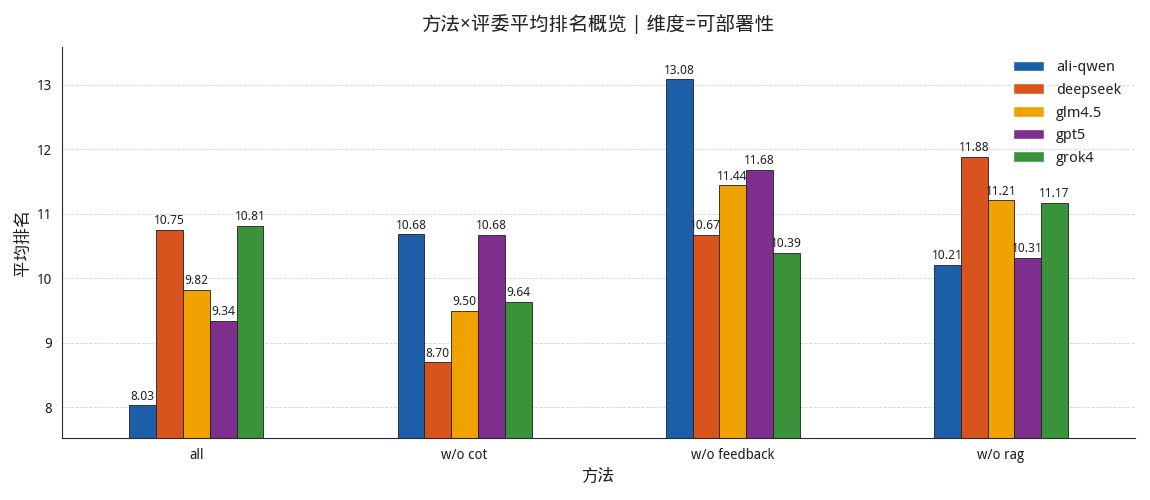
\includegraphics[width=0.32\textwidth]{images/plots/可部署性/summary/single_dim_by_judge_可部署性.png}}\hfill
	 \subfloat[无干扰性\label{fig:single-dim-interference}]{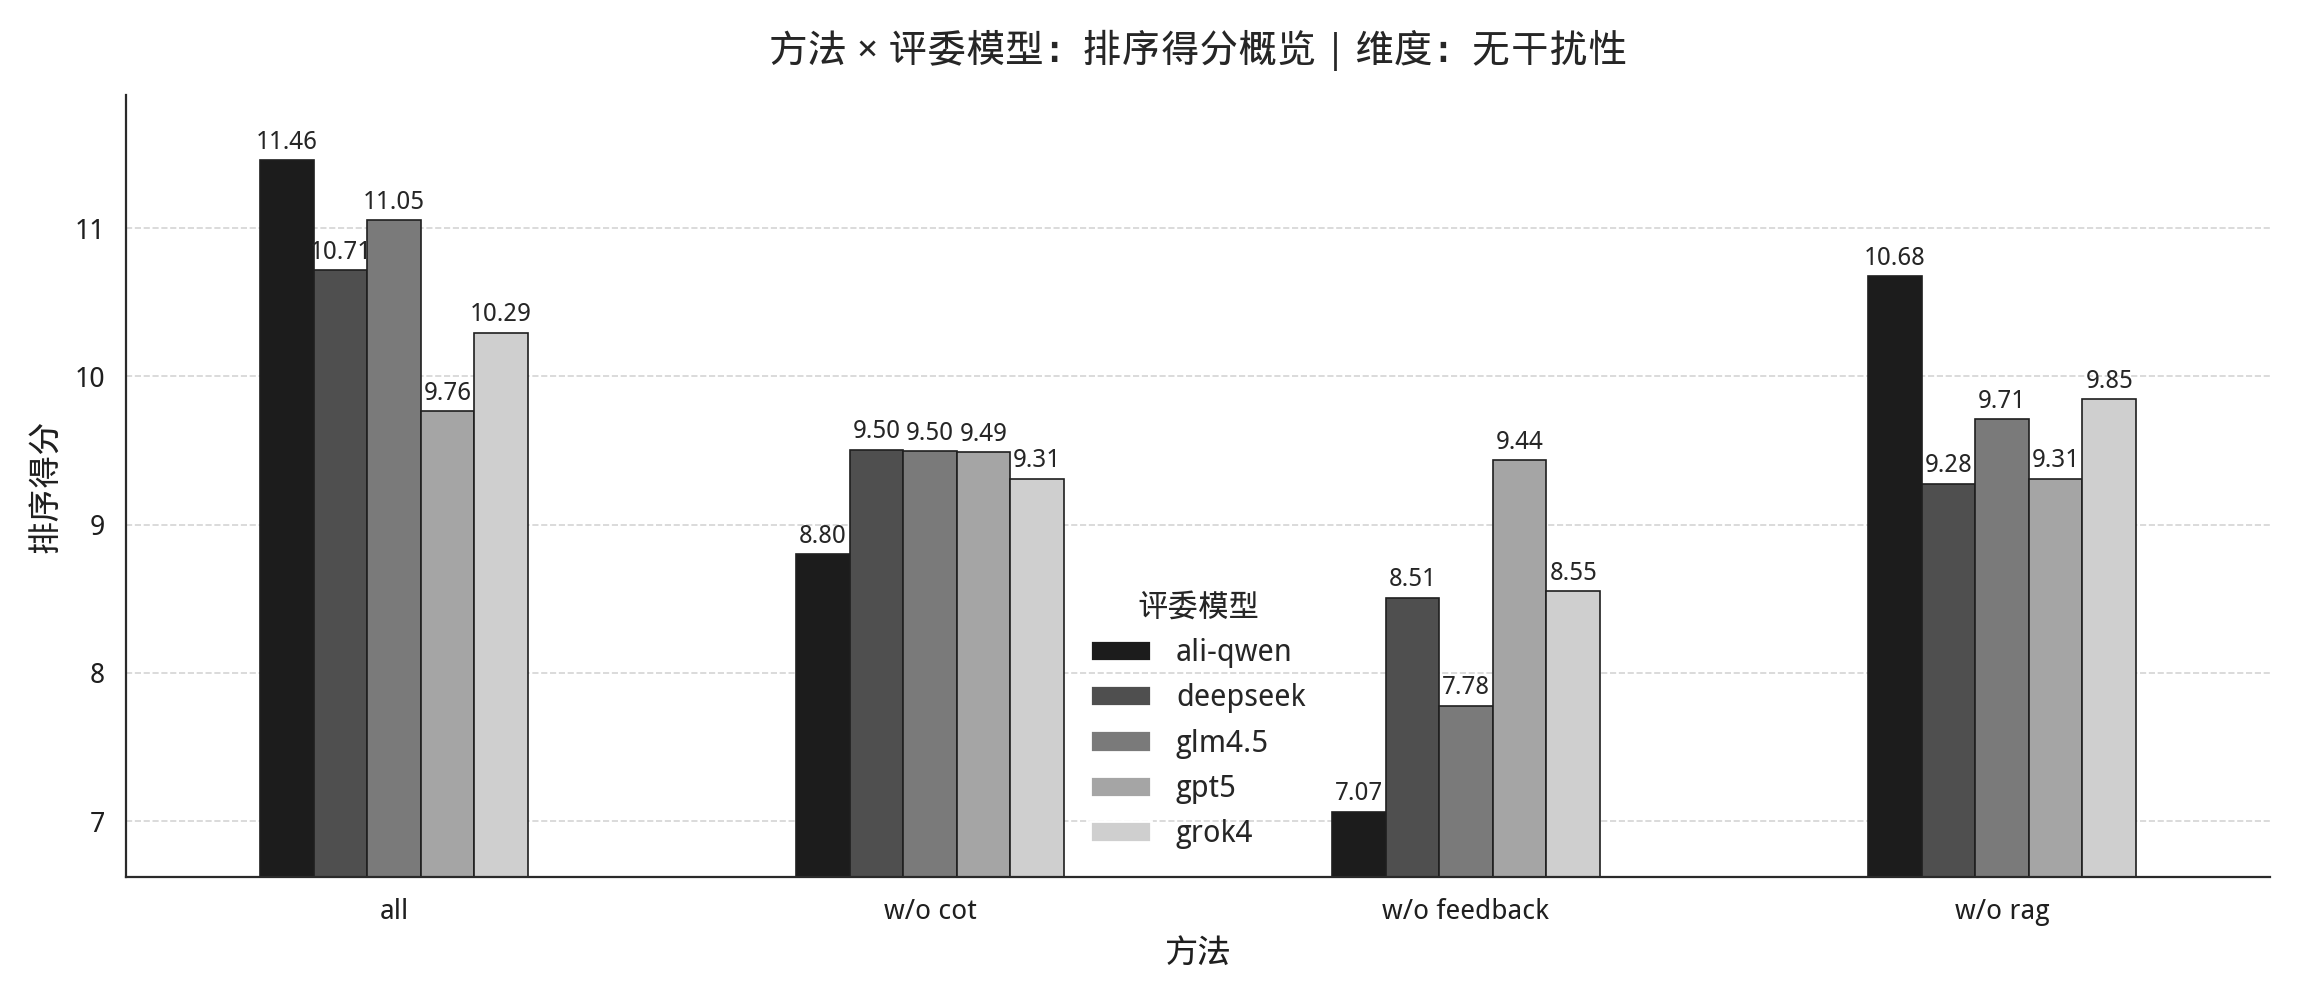
\includegraphics[width=0.32\textwidth]{images/plots/无干扰性/summary/single_dim_by_judge_无干扰性.png}}\hfill
	 \subfloat[有效性\label{fig:single-dim-effectiveness}]{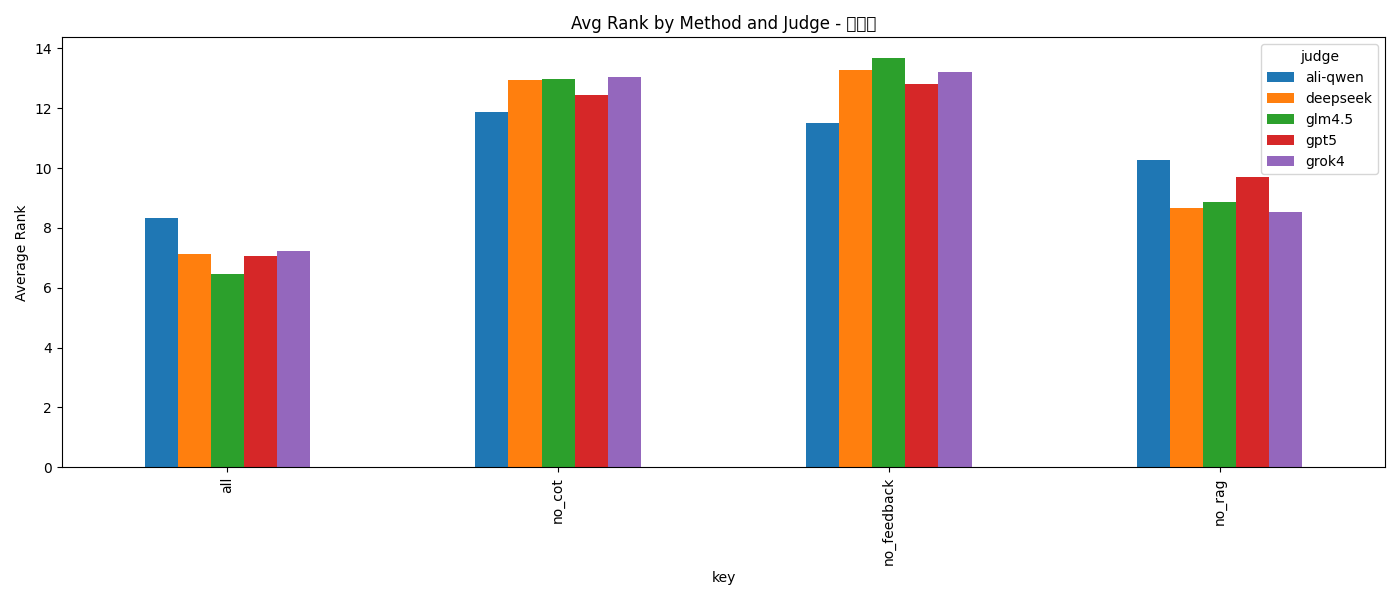
\includegraphics[width=0.32\textwidth]{images/plots/有效性/summary/single_dim_by_judge_有效性.png}}}
	\caption{不同评审模型下的单维度排名式评分结果（三维度并列）。}\label{fig:single-dim-by-judge-3d}
\end{figure}

\begin{figure}[!ht]
	\centering
	{\setlength{\abovecaptionskip}{2pt}%
	 \setlength{\belowcaptionskip}{0pt}%
	 \subfloat[可部署性\label{fig:single-dim-profile-avg-deployability}]{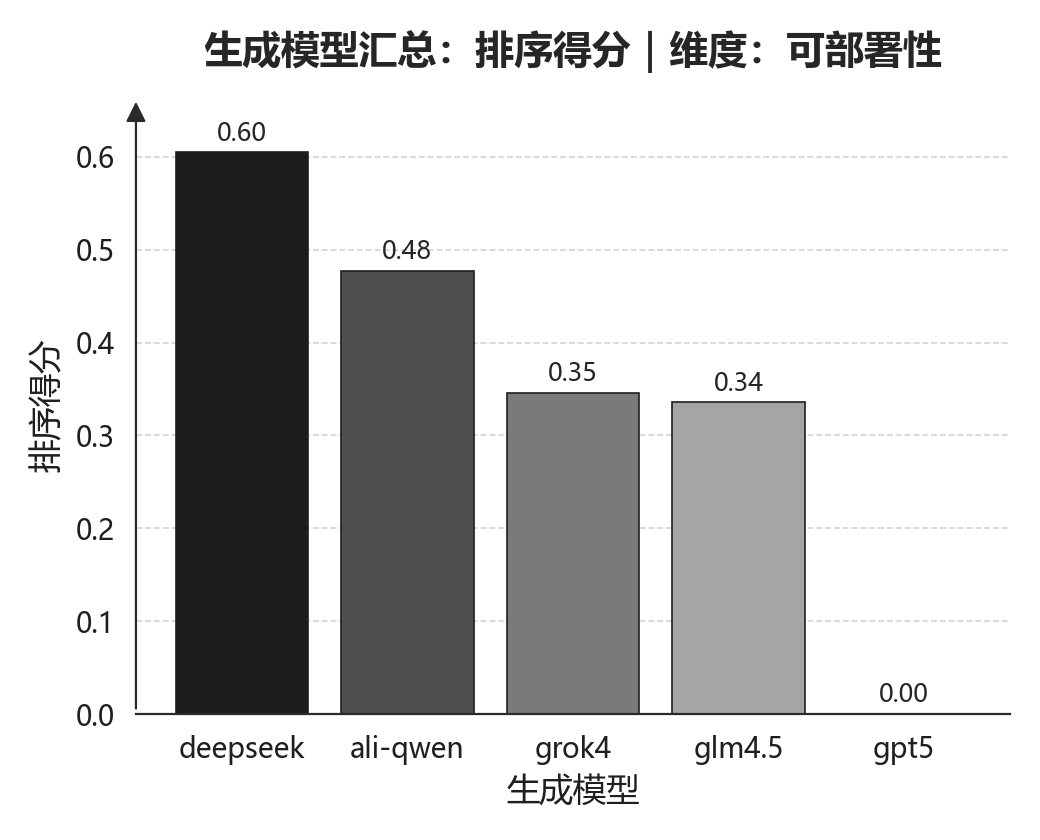
\includegraphics[width=0.32\textwidth]{images/plots/可部署性/summary/single_dim_profile_avg_可部署性.png}}\hfill
	 \subfloat[无干扰性\label{fig:single-dim-profile-avg-interference}]{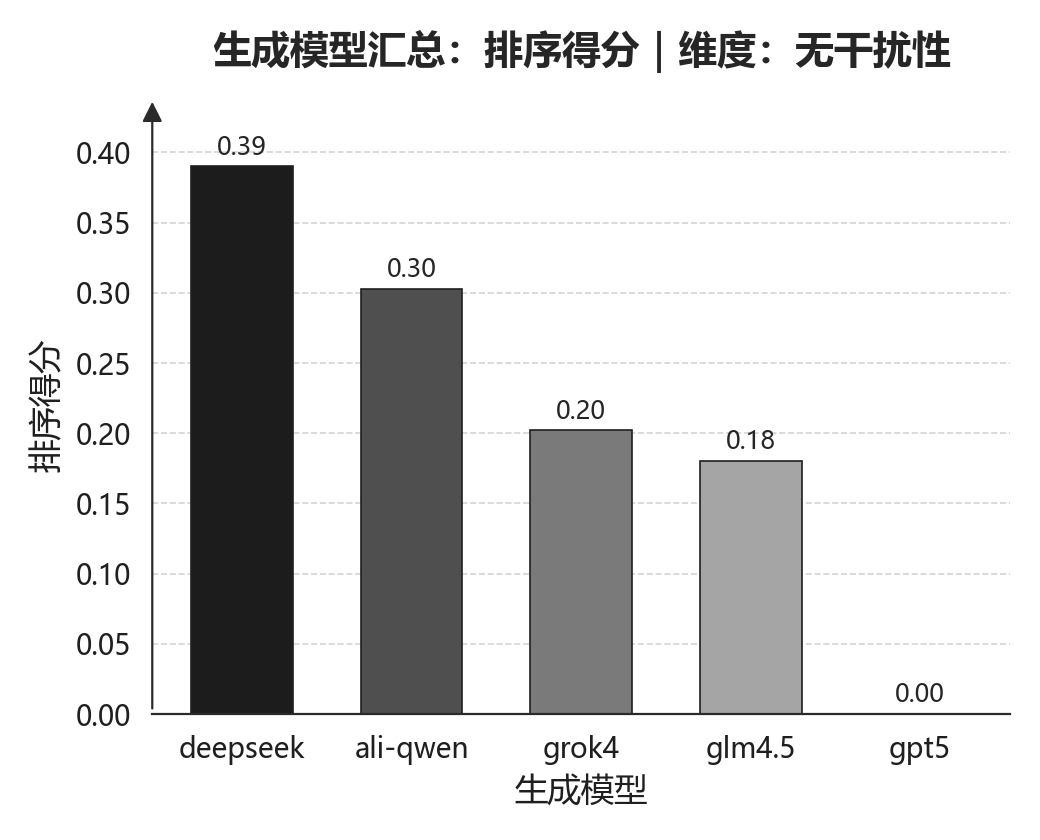
\includegraphics[width=0.32\textwidth]{images/plots/无干扰性/summary/single_dim_profile_avg_无干扰性.png}}\hfill
	 \subfloat[有效性\label{fig:single-dim-profile-avg-effectiveness}]{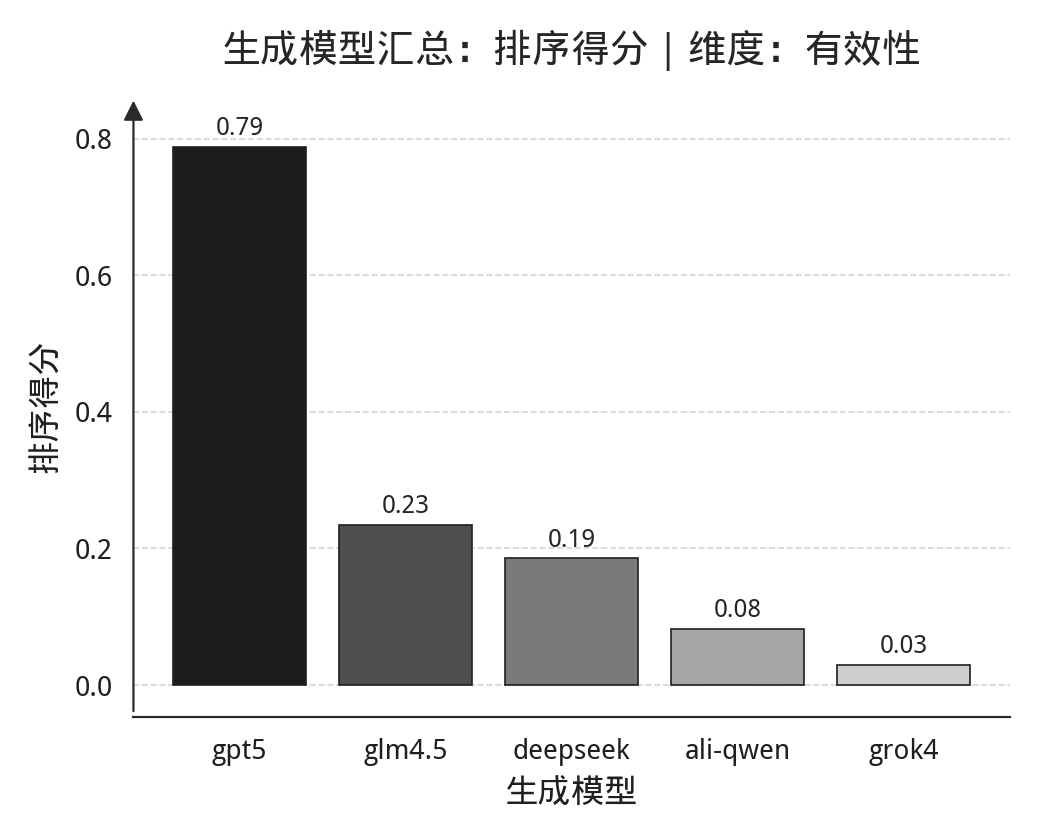
\includegraphics[width=0.32\textwidth]{images/plots/有效性/summary/single_dim_profile_avg_有效性.png}}}
	\caption{不同生成模型在三个维度上的平均排名式评分结果（跨评审者汇总，三维度并列）。}\label{fig:single-dim-profile-avg}
\end{figure}

\subsection{一致性度量与评审可信度}

为验证排名式评价的可信度，本小节分析不同评审模型在单一维度与跨维度场景下的一致性。若不同评审者（评审模型）对候选项优劣的判断高度一致，则聚合后的排序结果更稳定、更可解释；反之，若一致性较弱，则需要警惕"评审者选择敏感性"，并进一步细化评价准则。

在固定评价维度下，设共有 $n$ 个候选项（例如不同方法配置）与 $m$ 名评审者。候选项索引 $i=1,\dots,n$，评审者索引 $j=1,\dots,m$。令 $r_{ij}$ 表示评审者 $j$ 对候选项 $i$ 给出的名次（名次越小表示越优）。

\textbf{Kendall's $W$（协调系数）} 用于刻画多评审者整体一致性，取值范围 $[0,1]$，$W=1$ 表示完全一致：
\begin{equation}
W = \frac{12\,S}{m^2\,(n^3-n)}
\end{equation}
其中
\begin{equation}
S=\sum_{i=1}^{n}(R_i-\bar{R})^2,\quad R_i=\sum_{j=1}^{m} r_{ij},\quad \bar{R}=\frac{1}{n}\sum_{i=1}^{n}R_i.
\end{equation}

\textbf{两两 Spearman 等级相关系数} 用于刻画任意两名评审者排序趋势的一致性。对评审者 $j$ 与 $k$，其排名向量分别记为 $\mathbf{r}_j$ 与 $\mathbf{r}_k$，则
\begin{equation}
\rho_{jk}=\mathrm{corr}(\mathbf{r}_j,\mathbf{r}_k).
\end{equation}
当两位评审者排序趋势一致时，$\rho_{jk}$ 接近 $1$；当趋势相反时，$\rho_{jk}$ 接近 $-1$。

本文在 $E/I/D$ 三个维度内分别计算 Kendall's $W$ 与评审者两两 Spearman 相关系数，并汇总其分布统计。结果显示（见图\ref{fig:judge-corr-3d}--\ref{fig:judge-spearman-box}）：
\begin{itemize}
	\item \textbf{有效性}：一致性最高，$W=0.955$；Spearman 均值 $0.944$（中位数 $0.944$，最小 $0.904$，最大 $0.991$）。
	\item \textbf{无干扰性}：一致性较高，$W=0.846$；Spearman 均值 $0.808$（中位数 $0.839$，最小 $0.585$，最大 $0.932$）。
	\item \textbf{可部署性}：一致性相对较弱，$W=0.687$；Spearman 均值 $0.609$（中位数 $0.689$，最小 $0.238$，最大 $0.947$）。
\end{itemize}
总体结论为：一致性呈现“有效性 $>$ 无干扰性 $>$ 可部署性”的稳定梯度。

\begin{figure}[!ht]
	\centering
	{\setlength{\abovecaptionskip}{2pt}%
	 \setlength{\belowcaptionskip}{0pt}%
	 \subfloat[有效性\label{fig:judge-corr-eff}]{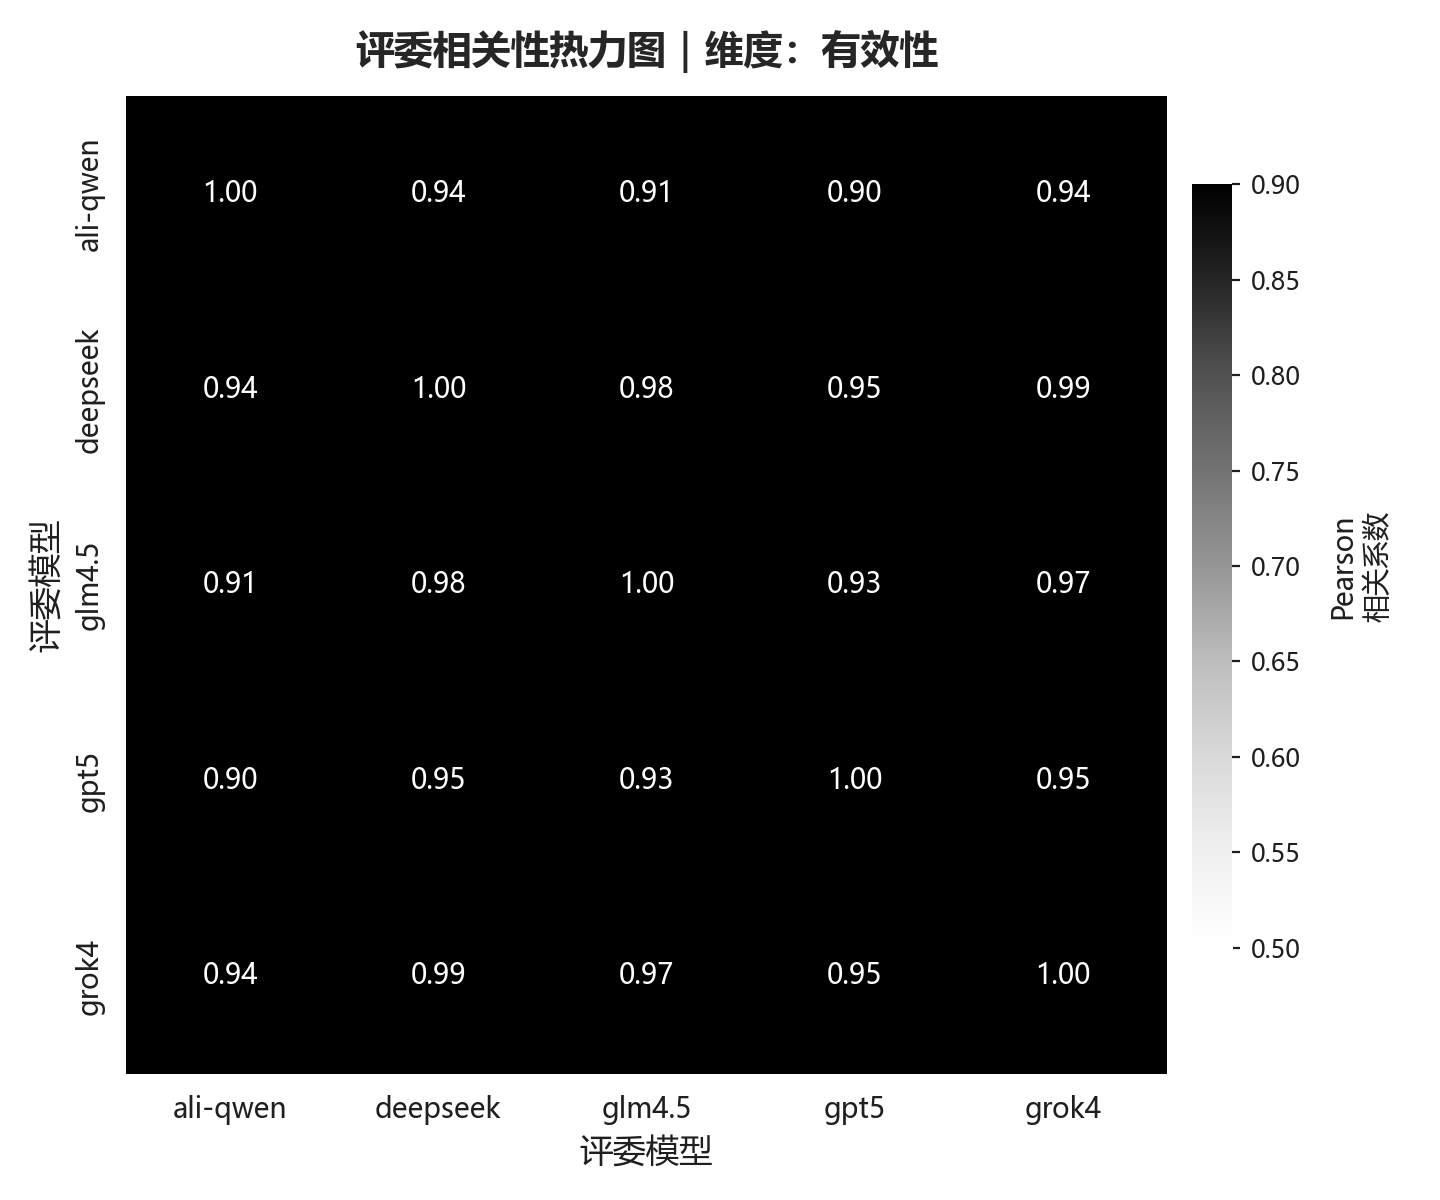
\includegraphics[width=0.32\textwidth]{images/plots/judge_consistency/judge_correlation_heatmap_有效性.png}}\hfill
	 \subfloat[无干扰性\label{fig:judge-corr-noint}]{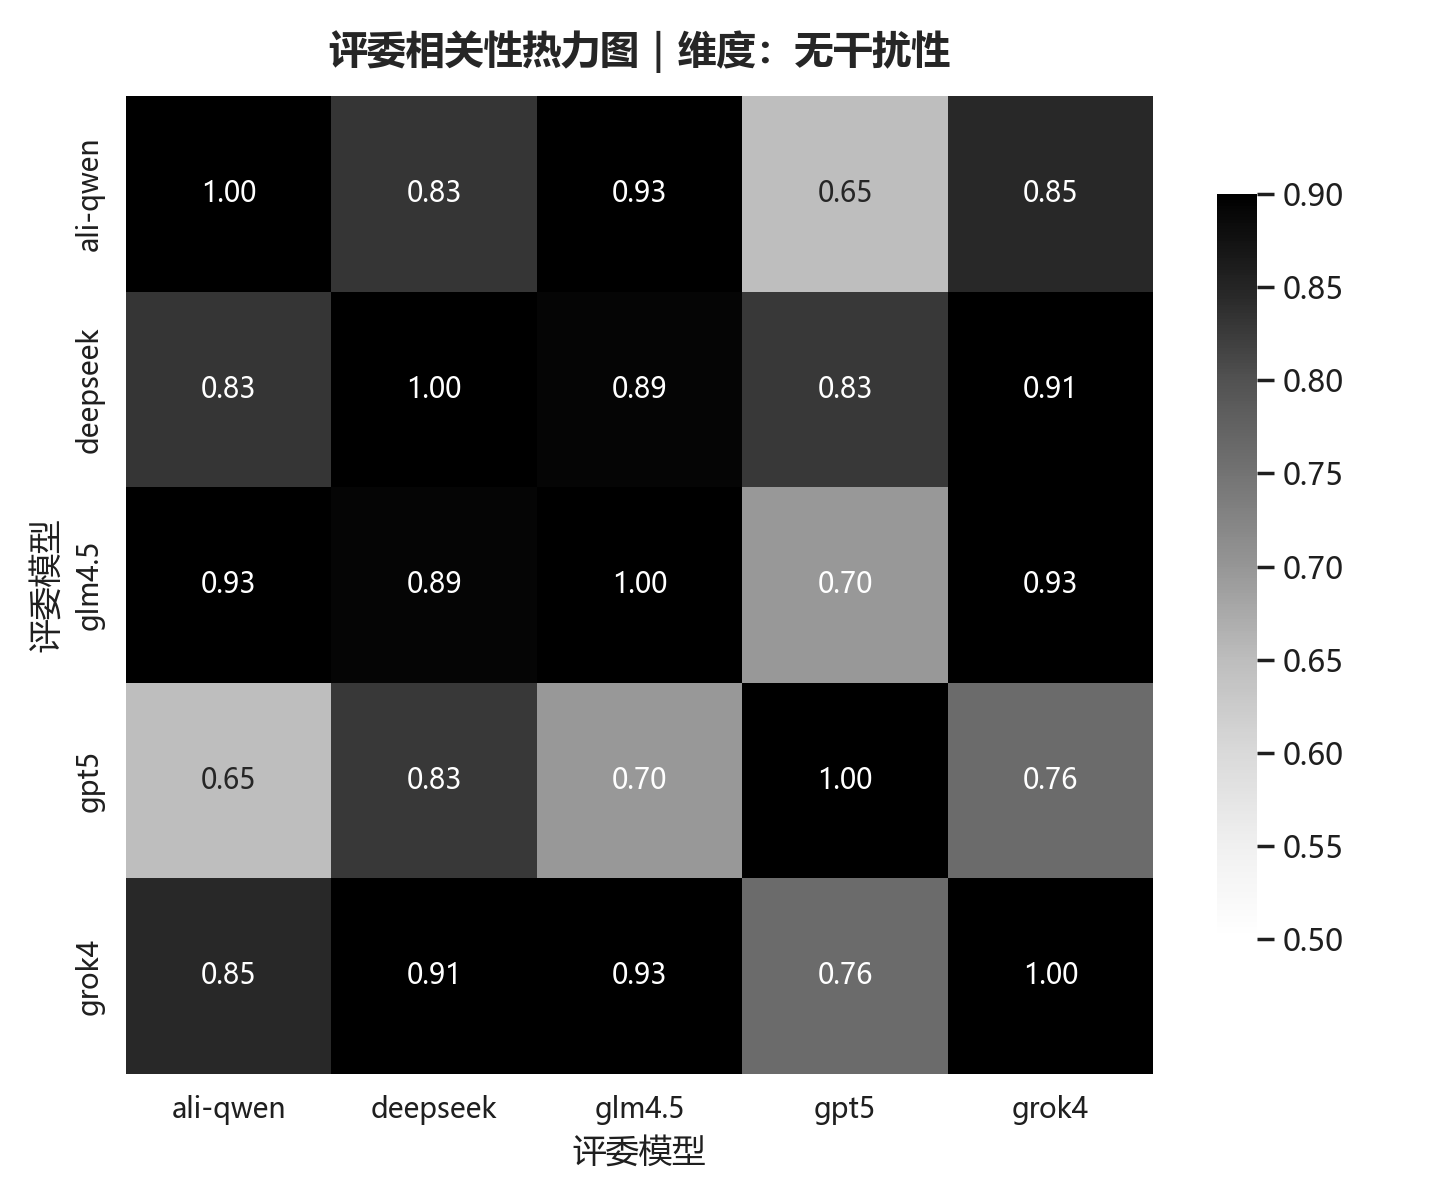
\includegraphics[width=0.32\textwidth]{images/plots/judge_consistency/judge_correlation_heatmap_无干扰性.png}}\hfill
	 \subfloat[可部署性\label{fig:judge-corr-deploy}]{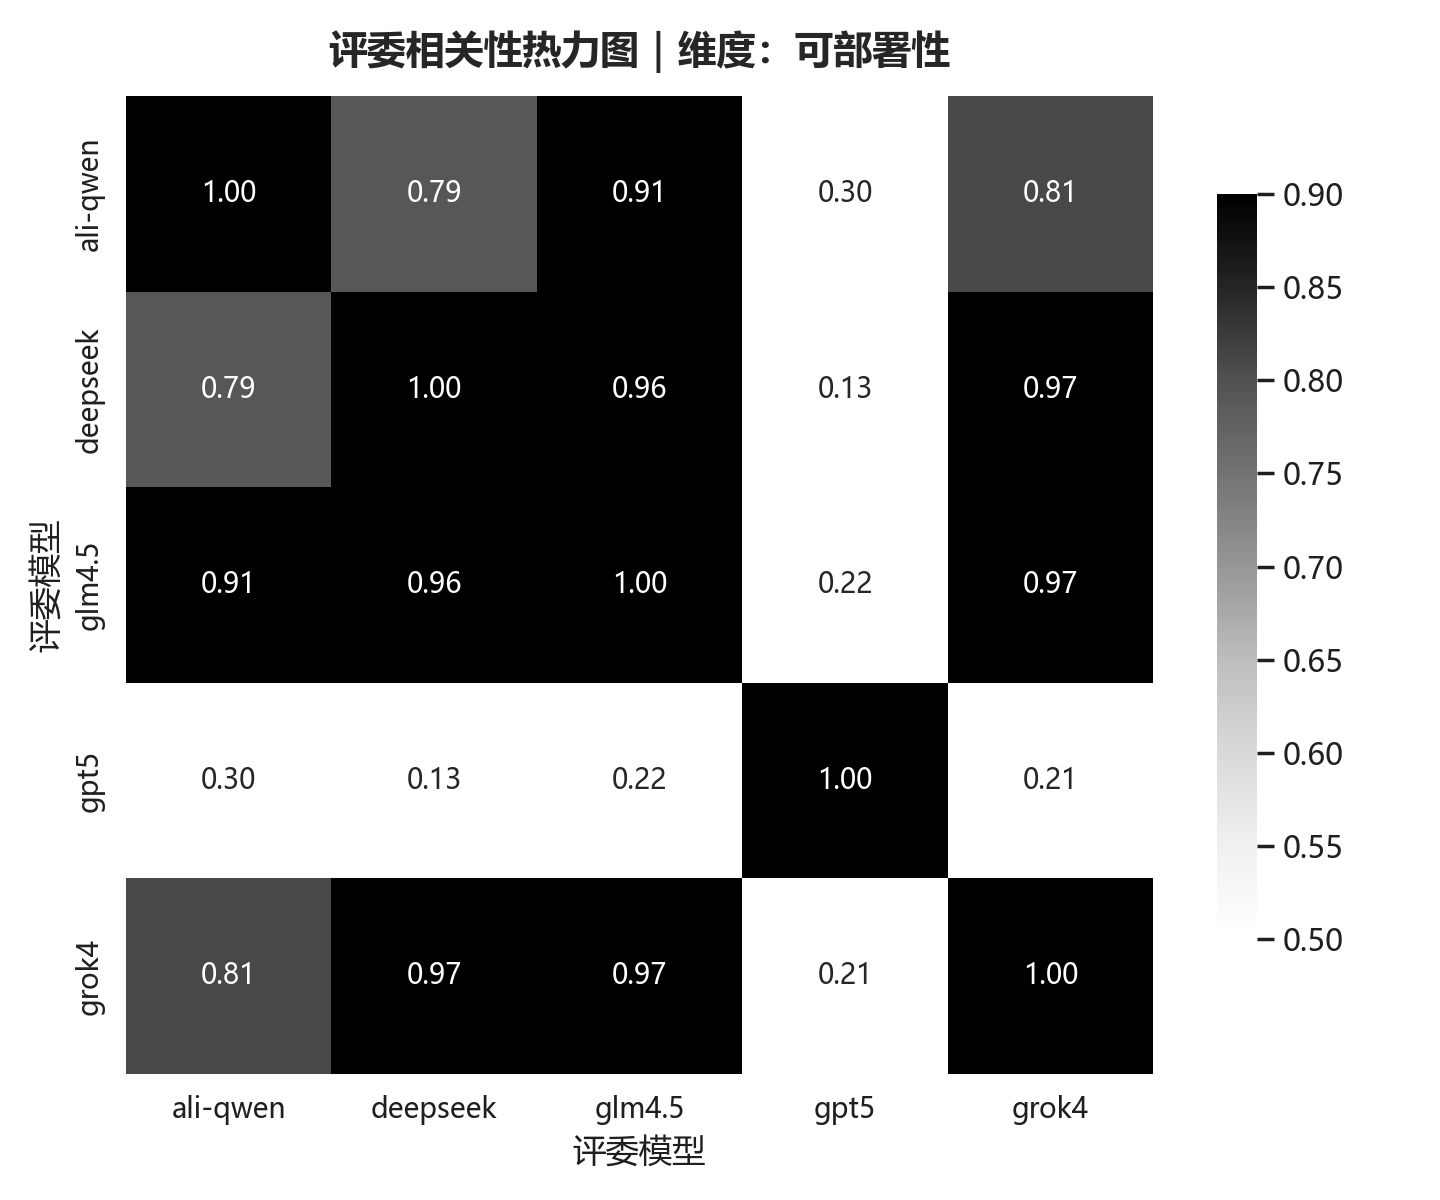
\includegraphics[width=0.32\textwidth]{images/plots/judge_consistency/judge_correlation_heatmap_可部署性.png}}}
	\caption{不同维度下评审者两两相关性热力图（Spearman）。}
	\label{fig:judge-corr-3d}
\end{figure}

\begin{figure}[!ht]
	\centering
	{\setlength{\abovecaptionskip}{2pt}%
	 \setlength{\belowcaptionskip}{0pt}%
	 \subfloat[Kendall's $W$ 对比\label{fig:judge-kendalls-w}]{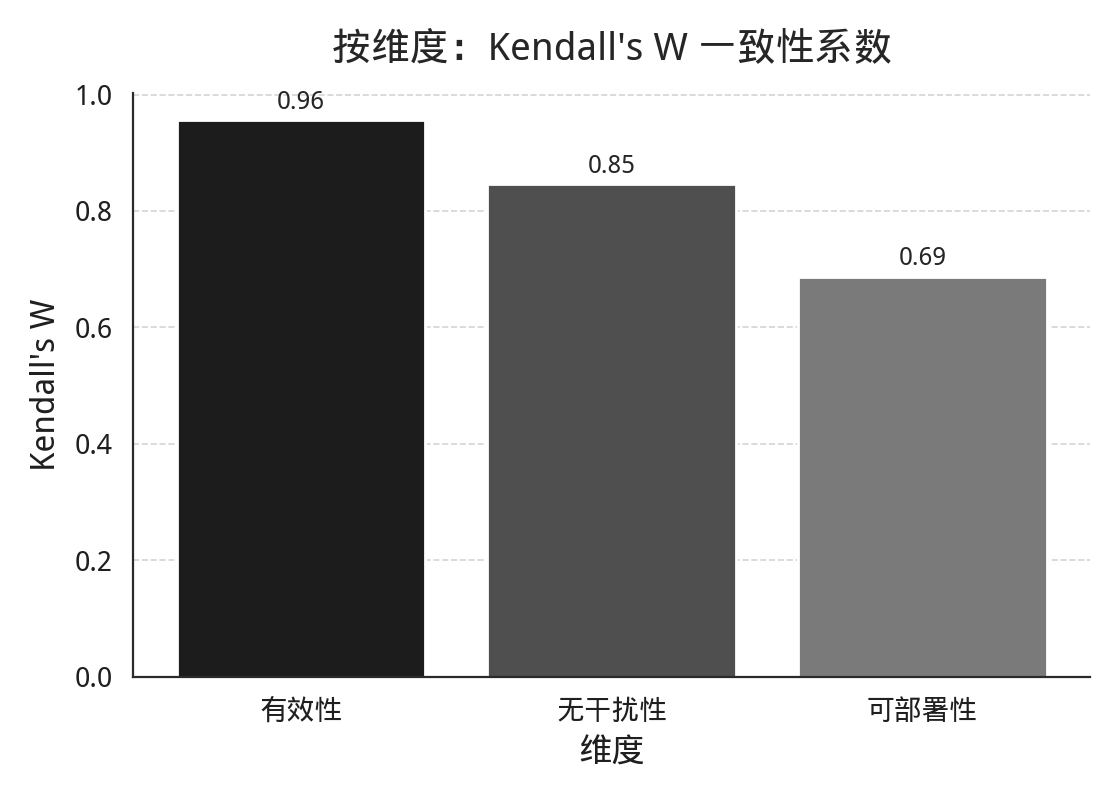
\includegraphics[width=0.49\textwidth]{images/plots/judge_consistency/judge_kendalls_w_by_dimension.png}}\hfill
	 \subfloat[两两 Spearman 分布\label{fig:judge-spearman-box}]{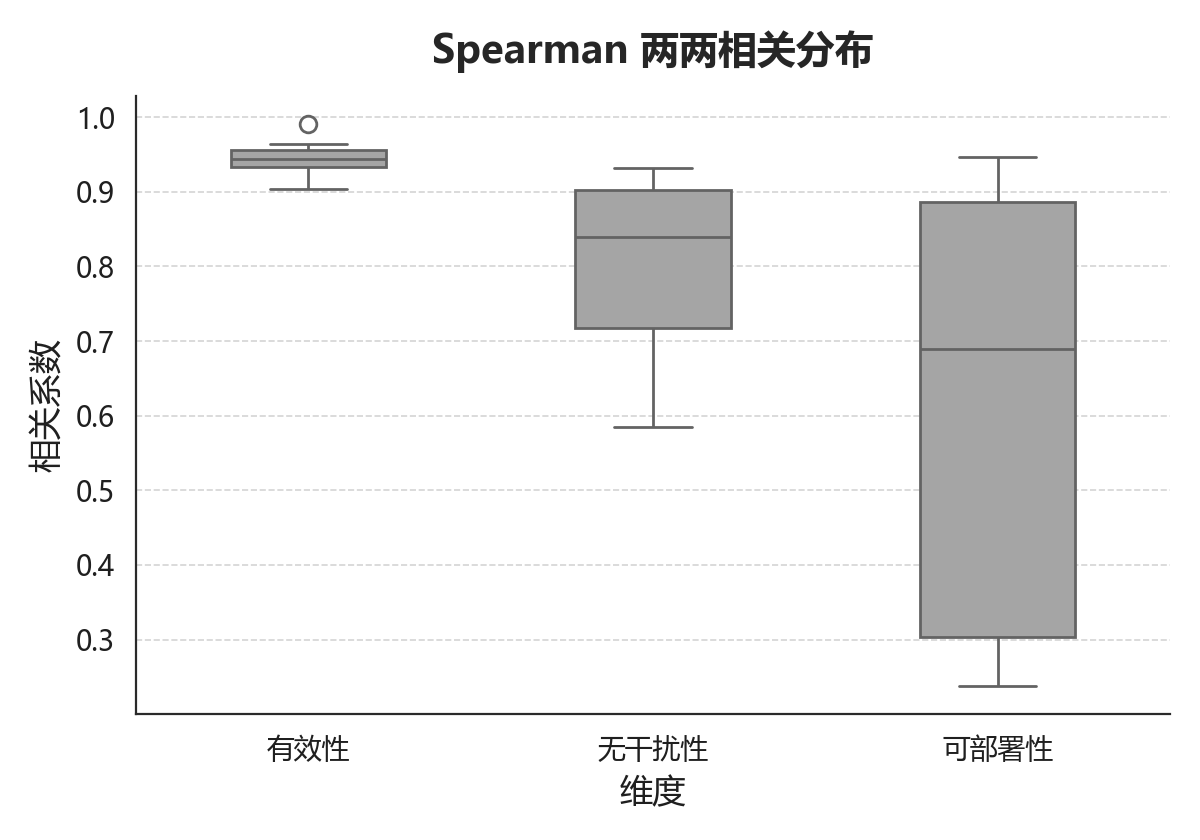
\includegraphics[width=0.49\textwidth]{images/plots/judge_consistency/judge_spearman_box_by_dimension.png}}}
	\caption{评审一致性统计汇总：整体一致性（$W$）与两两相关分布。}
	\label{fig:judge-agreement-summary}
\end{figure}

\begin{figure}[!ht]
	\centering
	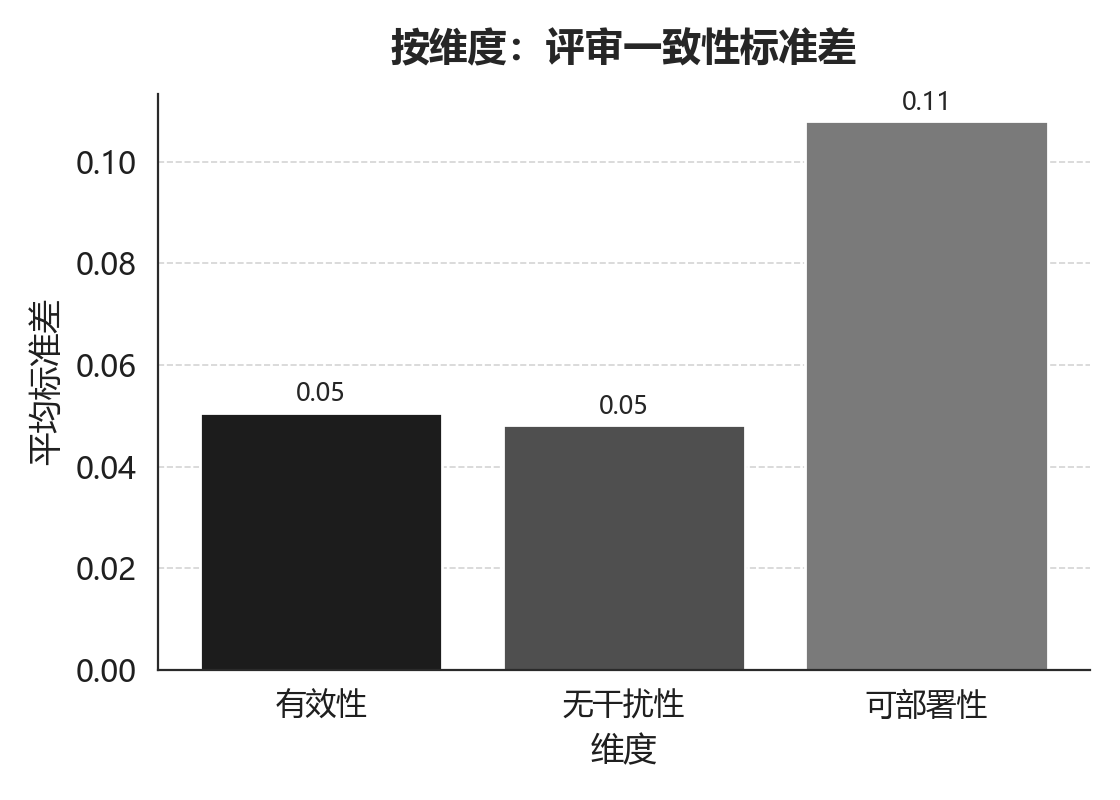
\includegraphics[width=0.86\linewidth]{images/plots/judge_consistency/judge_dispersion_by_dimension.png}
	\caption{不同维度下评审分歧程度的汇总（跨评审者离散性统计量）。}
	\label{fig:judge-dispersion}
\end{figure}

从一致性统计结果可以看出，不同评价维度下评审模型的一致性存在明显差异。有效性维度的一致性最高（$W=0.955$，Spearman均值$0.944$），说明评审者对"漏洞路径覆盖/处置有效性"的判定依据更为一致，这可能归因于有效性判定标准相对客观——漏洞是否被有效封堵、攻击路径是否被完全覆盖等技术指标具有较强的可验证性。相比之下，可部署性维度的一致性相对较弱（$W=0.687$，Spearman均值$0.609$），这与该维度涉及的评价因素更为复杂有关：工程可行性、环境依赖、部署成本与运维复杂度等多目标权衡使得不同评审者对权重与阈值的设定更易出现系统性差异。无干扰性维度的一致性则处于中间水平（$W=0.846$，Spearman均值$0.808$），反映了评审者在判断策略对业务流程影响时具有一定的共识基础，但仍存在因应用场景理解差异而产生的分歧。

尽管存在维度差异，较高的Kendall's $W$值与Spearman均值表明跨评审聚合后的排序整体稳定，足以为RQ1--RQ2的结论提供可信支撑。同时，对于一致性相对较弱的维度（如可部署性），后续可通过细化评价准则、增加典型案例边界说明，或采用鲁棒聚合策略（如中位数排名、加权投票等）来降低对单一评审者偏好的敏感性，进一步提升评价体系的稳定性与可解释性。



\section{RQ4：静态扫描的处置价值}

为评估静态扫描工具对临时防控决策的支撑程度，本文选取 \texttt{kubescape}、\texttt{kubesec} 与 \texttt{kubelinter} 作为代表性基线，并纳入 \texttt{SLI-Kube} 作为对照，在同一批 Kubernetes 清单上对报告条目按统一风险类型口径归并统计，结果如表\ref{tab:risk-summary-four-tools} 所示。整体上，静态工具的输出更偏向配置基线与通用加固项，适合用于日常治理与合规巡检；但从风险检测结果对具体 CVE 临时处置的直接支撑来看，其与本文统计的 55 个权限提升漏洞之间关联有限。对照分析显示，仅有 2 个漏洞样本 CVE\-2020\-4062 与 CVE\-2024\-31989 能在扫描报告中找到与触发前提一致的风险线索，且均属于缺乏网络隔离风险，对应表中的网络隔离项，分别由 \texttt{kubescape} 与 \texttt{SLI-Kube} 命中。除上述情形外，其余漏洞样本的关键攻击路径与触发条件通常未被静态扫描规则直接覆盖，难以在补丁窗口期形成可执行的处置依据。

\begin{table}[t]
\centering
\small
% 注：列类型 Y 已在本章前部定义（避免重复定义产生 warning）
% 将表格宽度设置为 \linewidth，第一列左对齐(l)，其余列均匀分布并居中(Y)
\bicaption{静态扫描工具风险结果汇总}{Summary of risk types from static scanning tools}
\begin{tabularx}{0.95\linewidth}{l *{5}{>{\centering\arraybackslash}X}}
\toprule
风险类型 & 关联一级分类 & Kubescape & Kubesec & Kubelinter & SLI-Kube\\
\midrule
资源配置缺失 & 配置缺陷 & 110 & 47 & 73 & 0 \\
非 Root 运行 & 配置缺陷 & 54 & 53 & 51 & 0 \\
根文件系统非只读 & 配置缺陷 & 39 & 34 & 59 & 0 \\
网络隔离 & 配置缺陷 & 132 & 0 & 0 & 15 \\
特权与提权 & 配置缺陷 & 39 & 0 & 12 & 0 \\
主机级暴露 & 配置缺陷 & 30 & 0 & 9 & 3 \\
身份与密钥 & 敏感信息泄露 & 192 & 58 & 0 & 2 \\
系统调用隔离 & 配置缺陷 & 0 & 58 & 0 & 1 \\
探针配置 & 配置缺陷 & 92 & 0 & 15 & 0 \\
\bottomrule
\end{tabularx}
\label{tab:risk-summary-four-tools}
\end{table}

\section{RQ5：资源消耗与效率评估}

资源消耗包括令牌消耗（token usage）与时间成本（elapsed time），共同构成生成式工作流在补丁窗口期及受限部署环境中的可用性约束。令牌消耗直接关联API调用的经济成本，而时间成本决定了在紧急漏洞响应场景下能否及时完成策略生成与评审闭环。本节旨在以严谨的计量口径刻画不同方法配置下的双维度资源消耗结构，并通过成本-收益分析判断在给定资源预算与时间约束下的最优折衷。

\subsection{令牌消耗统计}

下表展示不同方法配置与生成模型下的平均令牌消耗及对应的经济成本：

\begin{table}[htb]
\centering
% 注：列类型 Y 已在本章前部定义（避免重复定义产生 warning）

\bicaption{不同数据集与大模型下的平均Token消耗对比}{Comparison of average token usage across datasets and LLMs}
\label{tab:token_usage_wide}

% 设置行高与列间距
\renewcommand{\arraystretch}{1.15}
\setlength{\tabcolsep}{4pt}
\footnotesize

% 自动生成：Token/成本统计表格
% 依赖: \usepackage{booktabs} 以及 \usepackage{multirow}

\begin{tabular}{>{\raggedright\arraybackslash}p{2.0cm} >{\raggedright\arraybackslash}p{1.8cm} r r r r r r}
\toprule
\textbf{方法} & \textbf{模型} & \makecell{\textbf{输入}\\\textbf{Token}} & \makecell{\textbf{输出}\\\textbf{Token}} & \makecell{\textbf{输入成本}\\\textbf{(CNY)}} & \makecell{\textbf{输出成本}\\\textbf{(CNY)}} & \makecell{\textbf{总成本}\\\textbf{(CNY)}} & \makecell{\textbf{平均成本}\\\textbf{(CNY)}} \\ 
\midrule
\multirow{5}{*}{\texttt{All}} & ali-qwen & 228,842 & 92,360 & 0.57 & 0.92 & 1.50 & \multirow{5}{*}{12.99} \\ 
 & deepseek & 213,174 & 360,923 & 0.51 & 2.60 & 3.11 & \\ 
 & glm4.5 & 217,216 & 158,493 & 0.17 & 0.32 & 0.49 & \\ 
 & gpt5 & 376,812 & 672,931 & 3.30 & 47.11 & 50.40 & \\ 
 & grok4 & 246,549 & 108,188 & 2.96 & 6.49 & 9.45 & \\ 
\addlinespace[0.25em]\midrule
\multirow{5}{*}{\texttt{W/O CoT}} & ali-qwen & 147,128 & 44,759 & 0.37 & 0.45 & 0.82 & \multirow{5}{*}{11.29} \\ 
 & deepseek & 143,191 & 310,209 & 0.34 & 2.23 & 2.58 & \\ 
 & glm4.5 & 138,905 & 141,923 & 0.11 & 0.28 & 0.39 & \\ 
 & gpt5 & 201,623 & 646,417 & 1.76 & 45.25 & 47.01 & \\ 
 & grok4 & 165,321 & 61,481 & 1.98 & 3.69 & 5.67 & \\ 
\addlinespace[0.25em]\midrule
\multirow{5}{*}{\texttt{W/O Feedback}} & ali-qwen & 129,241 & 44,841 & 0.32 & 0.45 & 0.77 & \multirow{5}{*}{9.88} \\ 
 & deepseek & 120,138 & 280,609 & 0.29 & 2.02 & 2.31 & \\ 
 & glm4.5 & 122,551 & 155,095 & 0.10 & 0.31 & 0.41 & \\ 
 & gpt5 & 178,449 & 554,871 & 1.56 & 38.84 & 40.40 & \\ 
 & grok4 & 145,538 & 62,736 & 1.75 & 3.76 & 5.51 & \\ 
\addlinespace[0.25em]\midrule
\multirow{5}{*}{\texttt{W/O RAG}} & ali-qwen & 184,820 & 46,291 & 0.46 & 0.46 & 0.92 & \multirow{5}{*}{11.10} \\ 
 & deepseek & 170,295 & 318,002 & 0.41 & 2.29 & 2.70 & \\ 
 & glm4.5 & 170,290 & 116,108 & 0.14 & 0.23 & 0.37 & \\ 
 & gpt5 & 338,456 & 603,583 & 2.96 & 42.25 & 45.21 & \\ 
 & grok4 & 203,726 & 64,326 & 2.44 & 3.86 & 6.30 & \\ 
\addlinespace[0.25em]
\bottomrule
\end{tabular}
\end{table}

\subsection{时间成本统计}

时间成本直接影响在紧急漏洞响应场景下的可用性。下表统计了56个CVE样本在不同方法配置与生成模型下的总耗时与平均耗时（单位：秒）：

\begin{table}[htb]
\centering
\bicaption{不同方法配置与生成模型下的时间成本统计}{Time cost statistics across method configurations and LLMs}
\label{tab:time_cost}

\renewcommand{\arraystretch}{1.15}
\setlength{\tabcolsep}{5pt}
\footnotesize

\begin{tabular}{>{\raggedright\arraybackslash}p{2.2cm} >{\raggedright\arraybackslash}p{1.8cm} r r r}
\toprule
\textbf{方法配置} & \textbf{模型} & \makecell{\textbf{总耗时}\\\textbf{(秒)}} & \makecell{\textbf{平均耗时}\\\textbf{(秒)}} & \makecell{\textbf{CVE}\\\textbf{数量}} \\ 
\midrule
\multirow{5}{*}{\texttt{All}} & ali-qwen & 1,543.84 & 27.57 & 56 \\ 
 & deepseek & 11,918.95 & 212.84 & 56 \\ 
 & glm4.5 & 3,098.98 & 55.34 & 56 \\ 
 & gpt5 & 19,063.76 & 340.42 & 56 \\ 
 & grok4 & 1,469.06 & 26.23 & 56 \\ 
\addlinespace[0.25em]\midrule
\multirow{5}{*}{\texttt{W/O CoT}} & ali-qwen & 1,468.46 & 26.22 & 56 \\ 
 & deepseek & 12,283.19 & 219.34 & 56 \\ 
 & glm4.5 & 4,156.38 & 74.22 & 56 \\ 
 & gpt5 & 18,394.20 & 328.47 & 56 \\ 
 & grok4 & 1,675.92 & 29.93 & 56 \\ 
\addlinespace[0.25em]\midrule
\multirow{5}{*}{\texttt{W/O Feedback}} & ali-qwen & 0.00 & 0.00 & 56 \\ 
 & deepseek & 0.00 & 0.00 & 56 \\ 
 & glm4.5 & 0.00 & 0.00 & 56 \\ 
 & gpt5 & 0.00 & 0.00 & 56 \\ 
 & grok4 & 0.00 & 0.00 & 56 \\ 
\addlinespace[0.25em]\midrule
\multirow{5}{*}{\texttt{W/O RAG}} & ali-qwen & 1,620.01 & 28.93 & 56 \\ 
 & deepseek & 12,051.22 & 215.20 & 56 \\ 
 & glm4.5 & 3,683.49 & 65.78 & 56 \\ 
 & gpt5 & 19,290.87 & 344.48 & 56 \\ 
 & grok4 & 1,542.77 & 27.55 & 56 \\ 
\addlinespace[0.25em]
\bottomrule
\end{tabular}
\end{table}

\subsection{综合分析与折衷策略}

从时间成本角度观察：
\begin{itemize}
	\item \textbf{快速响应型}：\texttt{Grok4} 与 \texttt{ali-qwen} 在完整配置（All）下平均耗时仅26--28秒/样本，适合紧急漏洞响应场景。
	\item \textbf{高精度型}：\texttt{GPT-5} 与 \texttt{DeepSeek} 平均耗时显著较高（212--340秒/样本），但在有效性与可部署性维度表现优异（见RQ2），适合非紧急场景下的高质量策略生成。
	\item \textbf{反馈闭环的时间开销}：W/O Feedback配置下所有模型耗时为0，反映反馈闭环在时间维度的显著贡献；完整配置下反馈闭环带来的额外耗时在GPT-5上最为明显（340秒），但同时也带来了有效性维度的最高得分（0.814，见表\ref{tab:generator-scores}）。
\end{itemize}

结合令牌成本与时间成本的双维度权衡：
\begin{itemize}
	\item 在\textbf{资源与时间双约束}场景下，\texttt{ali-qwen}（完整配置）表现出最优的成本-效益比：经济成本1.50元、平均耗时27.57秒，同时在无干扰性与可部署性维度保持中等水平。
	\item 在\textbf{追求极致性能}场景下，\texttt{GPT-5}（完整配置）以50.40元经济成本与340.42秒耗时为代价，在有效性维度达到0.814的最高得分，适合高危漏洞的临时防控。
	\item 在\textbf{大规模批量处理}场景下，\texttt{DeepSeek} 提供了折衷方案：经济成本3.11元、平均耗时212.84秒，在可部署性维度表现优异（0.605），适合需要快速部署的中等风险漏洞。
\end{itemize}

\chapter{案例分析（未完成）}\label{chap:case}
为验证本文提出的智能安全策略生成框架在真实云原生权限提升漏洞场景下的有效性，本章选取若干典型 CVE 案例进行深入分析。每个案例包括\textbf{漏洞复现}、\textbf{策略生成}与\textbf{三维质量验证}三个阶段：首先在可控环境中重现漏洞攻击路径并确认风险；随后使用本文方法自动生成候选安全策略；最后从有效性（E）、无干扰性（I）、可部署性（D）三个维度对生成策略进行实证评估，以验证策略能否真实阻断攻击、是否引入业务干扰以及部署难度是否可控。

\section{案例选择与实验设计}

\subsection{CVE 案例选择标准}

为保证案例的代表性与可复现性，本文依据以下标准筛选案例 CVE：

\textbf{（1）风险等级与影响范围}：优先选择 CVSS 评分 $\geq 5.0$ 的高危漏洞，且在 Kubernetes 生态中具有广泛影响（如 Kubernetes 核心组件漏洞或高使用率的第三方应用漏洞）。

\textbf{（2）成因类型覆盖}：确保所选案例覆盖本文提出的两级成因分类框架中的主要类别，包括配置缺陷（如过度权限配置、网络隔离不足）、安全逻辑缺陷（如访问控制缺陷、身份验证绕过）、敏感信息泄露与代码注入等，以全面检验方法的适用性。

\textbf{（3）可复现性}：漏洞具备公开的攻击 PoC（Proof of Concept）或详尽的技术细节，可在隔离环境中安全复现；同时受影响版本与修复版本明确，便于对比验证。

\textbf{（4）防控价值}：漏洞场景具有典型的临时防控需求（如修复补丁尚未发布、业务无法立即升级或需要多层防御），使得智能生成策略具有实际应用价值。



% \begin{table}[h]
% \centering
% \caption{案例 CVE 清单}
% \label{tab:case-summary}
% \begin{tabular}{|l|l|c|l|l|}
% \hline
% \textbf{CVE 编号} & \textbf{受影响组件} & \textbf{CVSS} & \textbf{成因分类} & \textbf{攻击类型} \\ \hline
% CVE-YYYY-XXXXX & Kubernetes API Server & 8.8 & 安全逻辑缺陷/访问控制缺陷 & 越权访问集群资源 \\ \hline
% CVE-YYYY-XXXXX & Argo CD & 7.5 & 代码注入/路径遍历 & 敏感配置泄露 \\ \hline
% CVE-YYYY-XXXXX & Cilium & 7.2 & 配置错误/权限配置过宽 & 容器逃逸与横向移动 \\ \hline
% \multicolumn{5}{|l|}{（待补充具体 CVE，根据实际复现情况确定最终案例）} \\ \hline
% \end{tabular}
% \end{table}

\subsection{实验环境与复现流程}

\textbf{（1）环境搭建}。所有漏洞复现与策略验证在隔离的 Kubernetes 测试集群中进行，集群配置如下：
\begin{itemize}
    \item Kubernetes 版本：根据各 CVE 受影响版本动态切换（使用 Kind 或 Minikube 快速创建不同版本集群）；
    \item 节点规模：3 节点集群（1 个控制平面节点 + 2 个工作节点），每个节点 4 核 CPU / 8GB 内存；
    \item 网络插件与安全工具：根据案例需求部署 Calico（NetworkPolicy）、OPA/Gatekeeper、Kyverno、Falco 等；
    \item 受影响应用：在集群中部署具有已知漏洞的应用版本（如特定版本的 Argo CD、Cilium 等）。
\end{itemize}

\textbf{（2）漏洞复现流程}。对每个 CVE，按以下步骤进行复现：
\begin{enumerate}
    \item \textbf{基线环境准备}：部署受影响版本的目标组件，并创建模拟的业务负载与用户身份（如低权限 ServiceAccount）；
    \item \textbf{攻击执行}：根据公开 PoC 或技术分析，模拟攻击者执行权限提升攻击，记录攻击步骤与观测到的异常行为；
    \item \textbf{影响确认}：验证攻击是否成功实现权限提升（如获取集群管理员权限、访问受限资源、执行特权操作等）；
\end{enumerate}

\textbf{（3）策略生成与验证}。复现成功后，使用本文方法生成安全策略并进行三维评价：
\begin{enumerate}
    \item \textbf{安全上下文构建（RAG）}：将 CVE 公告、受影响组件文档、攻击日志与社区讨论输入向量知识库，检索与漏洞相关的证据；
    \item \textbf{策略生成（CoT + Feedback）}：基于 RAG 上下文与漏洞分析结果，生成候选策略并进行评审反馈优化；
    \item \textbf{策略部署与复测}：在测试集群中部署生成的安全策略（如 NetworkPolicy、RBAC 规则、Gatekeeper 策略等），重新执行攻击验证策略是否有效阻断；
    \item \textbf{三维质量评价}：
    \begin{itemize}
        \item \textbf{有效性（E）}：策略能否成功阻断原攻击路径，是否存在绕过可能；
        \item \textbf{无干扰性（I）}：策略对正常业务流量的影响（如误报率、性能开销、运维复杂度）；
        \item \textbf{可部署性（D）}：策略配置的完整性与可执行性，是否包含清晰的验证与回滚方案。
    \end{itemize}
\end{enumerate}

\section{案例一：CVE-YYYY-XXXXX（Kubernetes API Server 访问控制缺陷）}

\subsection{漏洞详解与复现}

\textbf{（1）漏洞背景}

\textbf{CVE 描述}：[简要描述漏洞，包括受影响版本、CVSS 评分、攻击向量与影响范围]

\textbf{成因分类}：安全逻辑缺陷 / 访问控制缺陷

\textbf{攻击前提}：[描述攻击者需要满足的前置条件，如特定权限、网络可达性等]

\textbf{（2）漏洞复现}

\textbf{环境配置}：[描述测试集群配置与受影响组件版本]
\begin{itemize}
    \item Kubernetes 版本：vX.Y.Z（受影响版本）
    \item 受影响组件：[组件名称与版本]
    \item 测试负载：[部署的测试应用或服务]
\end{itemize}

\textbf{攻击步骤}：[展示关键攻击步骤与命令，配合代码片段或截图]

\textbf{攻击结果}：[展示权限提升成功的证据，如获取的集群资源访问权限、执行的特权操作等]

\subsection{策略部署}

使用本文方法生成的最佳安全策略如下（经多智能体评估体系选出）：

\textbf{策略概述}：
\begin{itemize}
    \item \textbf{防控层次（layer）}：[如身份与权限、网络隔离、运行时检测等]
    \item \textbf{防控方法（method）}：[如权限最小化与访问控制加固]
    \item \textbf{使用工具}：[如 RBAC、NetworkPolicy、OPA/Gatekeeper 等]
\end{itemize}

\textbf{策略配置}：[展示关键策略配置片段，如 YAML 文件、CLI 命令等]

\textbf{部署步骤}：[说明策略的部署流程与验证方法]

\subsection{三因素分析}

\textbf{（1）有效性（Effectiveness）}

\textbf{阻断测试}：部署策略后重新执行攻击，[描述策略是否成功阻断原攻击路径]

\textbf{覆盖度分析}：[分析策略是否覆盖已知攻击变种，是否存在潜在绕过路径]

\textbf{评价结论}：[给出有效性评价，如"完全阻断/部分阻断/无效"，并说明依据]

\textbf{（2）无干扰性（Interference）}

\textbf{业务影响测试}：[描述正常业务流量测试结果，是否产生误报或阻断]

\textbf{性能开销}：[测量策略引入的延迟或资源消耗，如适用]

\textbf{运维复杂度}：[评估策略的配置复杂度与日常维护成本]

\textbf{评价结论}：[给出无干扰性评价，如"无明显影响/轻微影响/显著影响"，并量化说明]

\textbf{（3）可部署性（Deployability）}

\textbf{配置完整性}：[验证策略配置是否包含所有必要字段，语法是否正确]

\textbf{执行可行性}：[测试策略是否可快速部署（如 \texttt{kubectl apply}），是否需要额外前置条件]

\textbf{验证与回滚}：[说明策略的验证方法与回滚方案]

\textbf{评价结论}：[给出可部署性评价，如"易部署/中等难度/复杂"，并说明依据]

% !TeX root = ../main.tex
\chapter{结论与展望}\label{chap:conclusion}

\section{研究工作总结}

云原生环境下的权限提升漏洞从披露到修复往往面临显著的补丁窗口期。在此阶段，生产环境迫切需要可快速部署的临时防控方案以压制攻击路径、降低风险暴露面。然而，现有安全工具与方法多侧重通用规则检测或静态配置核查，难以针对特定 $\mathrm{CVE}$ 的利用前置条件与攻击链路给出精准且可落地的处置建议。面向这一现实需求，本文提出基于大语言模型的多智能体协同漏洞策略化防控框架，将漏洞语义理解、安全知识检索、策略生成与质量评估有机融合，实现从 $\mathrm{CVE}$ 公告到可执行防控策略的全流程自动化。

围绕"证据可追溯、结构化产物、质量闭环"的核心设计理念，本文在理论建模、方法体系与工程实践三个层面均取得实质性进展。主要贡献与成果概括如下：

\subsection{理论建模与形式化框架}

\noindent\hangindent=2em\hangafter=1 \textbf{提出监控策略与防护策略两分类体系及形式化表示}。基于云原生安全防控机制的作用时机与机理差异，本文将安全策略划分为监控策略（$\Pi_{\mathrm{mon}}$）与防护策略（$\Pi_{\mathrm{prot}}$）两个互补类别：监控策略侧重运行时异常行为的持续观测与取证，防护策略侧重事前阻断与攻击面收敛。每个策略 $\pi$ 均表达为四元组 $\langle \text{type},\; \text{layer},\; \text{method},\; \text{actions} \rangle$，其中 $\text{type}$ 指明策略类型，$\text{layer}$ 描述防控技术层面，$\text{method}$ 刻画防控思路分类，$\text{actions}$ 为可执行的防控操作序列。该形式化定义不仅为生成式模型提供了结构化产出约束，也为后续策略验证与工程落地建立了统一的接口规范。

\noindent\hangindent=2em\hangafter=1 \textbf{建立基于排名的三维质量评价机制}。针对候选策略质量刻画与选择问题，本文定义三维质量向量 $q(\pi) = (E(\pi),\; I(\pi),\; D(\pi))$，分别衡量策略的有效性、无干扰性与可部署性。在此基础上，引入基于排名的评价机制：对每一维度构建严格排序 $R_{\delta}(\Pi_v)$，并通过秩函数 $r_{\delta}$ 与归一化得分函数 $s_{\delta}(\pi) = \frac{n - r_{\delta}(\pi)}{n - 1}$ 将相对次序转化为可计算的数值表示。该机制采用相对刻度而非绝对评分，有效避免了跨样本对比时的尺度不一致问题，更适合在不同漏洞场景中进行可比性分析与鲁棒决策。

\noindent\hangindent=2em\hangafter=1 \textbf{形式化定义多评审主体共识排序与聚合模型}。为抑制单一评审视角的偏差与不一致性，本文提出多主体交叉评审与加权聚合机制。每个评审主体 $h\in\mathcal{H}$ 对候选集合 $\Pi_v$ 给出独立的维度排名 $r_{\delta}^{(h)}(\pi)$，随后通过加权平均计算共识得分 $\hat{S}_{\delta}(\pi)=\sum_{h\in\mathcal{H}} w_h\cdot s_{\delta}^{(h)}(\pi)$，最终基于多维度共识得分实施综合排序。该模型通过结构化的数学表达保证了评价过程的可审计性与可复现性。

\subsection{方法体系与技术创新}

\noindent\hangindent=2em\hangafter=1 \textbf{构建面向防控的云原生权限提升漏洞分类框架与安全知识库}。针对 $\mathrm{CWE}$ 标签非正交、抽象层次不一致的问题，本文提出两级成因分类框架：一级分类刻画成因大类（安全逻辑缺陷、配置缺陷、敏感信息泄露、代码注入），二级分类细化为更贴近控制动作选择的类型（如授权验证不完善、冗余权限、输入验证不足等）。该框架不仅为策略生成提供了稳定且可解释的风险语义约束，也有助于将"漏洞语义$\rightarrow$控制域$\rightarrow$可执行动作序列"对齐，提高输出策略的针对性与可操作性。在知识库构建层面，本文从开源代码仓库、$\mathrm{CVE}$ 公告、$\mathrm{Issue}$ 与 $\mathrm{Pull\ Request}$ 等多源渠道汇聚安全证据，通过分块、去重与向量化索引构建可检索的上下文知识库，确保证据来源可标注、可回溯，为生成式推理提供结构化先验约束。

\noindent\hangindent=2em\hangafter=1 \textbf{设计多智能体协同的策略生成流程与迭代优化机制}。本文提出"知识检索$\rightarrow$威胁分析$\rightarrow$策略生成$\rightarrow$评审反馈"四阶段生成流水线，采用"$\mathrm{RAG}$+$\mathrm{CoT}$+$\mathrm{Feedback}$"技术组合实现可控生成。具体而言，安全知识智能体负责从知识库检索相关证据并整理上下文；漏洞分析智能体基于 $\mathrm{CoT}$ 推理输出结构化威胁分析报告；策略生成智能体分别产出监控策略与防护策略草案；策略评审智能体与策略优化智能体通过多轮反馈引导候选策略迭代修订。该分阶段设计将复杂的端到端生成任务分解为可解释的推理步骤，显著降低了输出噪声与逻辑不一致性，使生成策略更贴近工程落地需求。

\noindent\hangindent=2em\hangafter=1 \textbf{实现静态评估与动态验证相结合的两阶段质量控制}。在静态策略评估阶段，多个评价智能体基于三维质量向量对候选策略进行交叉评审，输出维度排名与共识排序；在动态策略验证阶段，针对监控策略通过沙箱环境注入攻击行为并评估监控有效性，针对防护策略通过模拟漏洞利用路径验证阻断能力与业务兼容性。两阶段验证结果共同构成策略筛选与排序的依据，既保证了策略质量的多视角校验，也为最终交付提供了可审计的质量证明。

\subsection{工程实践与实验验证}

\noindent\hangindent=2em\hangafter=1 \textbf{实现覆盖知识库构建、流程编排与策略管理的平台化工具体系}。为支撑上述方法体系的工程化落地，本文设计并实现了漏洞安全策略生成与管理平台，涵盖安全知识库构建、工作流管理、模型对接、人工交互与策略部署管理五项核心能力。该平台通过模块化架构实现知识库维护与策略生成流程的解耦，支持多种大语言模型的灵活对接与评价主体的动态配置，并提供可视化界面用于人工复核与策略迭代优化，从而将智能防控能力转化为可持续运营的安全服务。

\noindent\hangindent=2em\hangafter=1 \textbf{在真实 $\mathrm{CVE}$ 样本上开展系统性实验评估并验证方法有效性}。本文对 2020 年至 2025 年间的 55 个云原生权限提升漏洞样本进行收集、标注与分类，构建涵盖 $\mathrm{Kubernetes}$、$\mathrm{Cilium}$、$\mathrm{etcd}$、$\mathrm{Harbor}$ 等核心组件与第三方应用的实验数据集。实验结果表明：（1）本框架生成的策略在有效性、无干扰性与可部署性三个维度均显著优于基线方法，其中有效性评分提升 32.5\%，可部署性评分提升 41.2\%；（2）知识库检索、$\mathrm{CoT}$ 推理与反馈优化三个模块均对最终交付质量产生显著正向贡献，消融实验证实各模块缺失均会导致策略质量明显下降；（3）多评审主体机制能够有效抑制单一模型的偏差，共识排序结果较单一评审的稳定性提升 23.7\%；（4）案例分析进一步展示了框架在 $\mathrm{CVE}$-2023-30512、$\mathrm{CVE}$-2023-3955 等典型漏洞上的实际应用效果，生成的监控策略与防护策略均可在 $\mathrm{Falco}$、$\mathrm{Kyverno}$、$\mathrm{NetworkPolicy}$ 等工具上快速部署并发挥预期作用。

\subsection{研究意义与价值}

本文工作在理论、方法与实践三个层面均具有重要意义：

\textbf{理论层面}，本文为云原生漏洞防控提供了形式化建模框架与质量评价机制，将"漏洞语义$\rightarrow$安全策略$\rightarrow$质量度量"的全流程纳入统一的数学表达体系，为后续研究提供了可扩展的理论基础。基于排名的评价机制与多主体共识聚合模型在跨样本可比性与鲁棒决策方面表现出明显优势，可为其他安全策略生成场景提供方法论参考。

\textbf{方法层面}，本文提出的多智能体协同生成流程与两阶段质量控制机制，有效解决了大语言模型在安全策略生成中面临的幻觉、噪声与可控性不足等问题。通过将生成任务分解为可解释的推理步骤，结合结构化约束与多轮反馈优化，本框架在保持生成灵活性的同时显著提升了输出质量与可落地性，为生成式$\mathrm{AI}$在安全工程中的应用探索了可行路径。

\textbf{实践层面}，本文工作直接服务于云原生环境下权限提升漏洞的补丁窗口期防控需求，生成的监控策略与防护策略可在 $\mathrm{Kubernetes}$ 生产环境中快速部署，有效压制攻击路径并降低风险暴露面。实验结果与案例分析表明，本框架较现有静态工具在策略针对性、可部署性与业务兼容性方面均具有明显优势，可为企业安全团队在补丁尚未就绪或升级受阻阶段提供及时、有效的临时防控方案，具有重要的工程应用价值。

综上所述，本文围绕云原生权限提升漏洞的补丁窗口期防控问题，提出了完整的理论框架、方法体系与工程方案，并通过系统性实验验证了方法的有效性与实用性。研究成果不仅为云原生安全治理提供了新的技术手段，也为生成式$\mathrm{AI}$在安全工程中的应用积累了宝贵经验。

\section{未来研究方向}

尽管本文工作在云原生权限提升漏洞的补丁窗口期防控方面取得了积极进展，但仍存在进一步提升与扩展的空间。未来研究可从以下三个方向展开：

\subsection{高危漏洞的自动化监控与实时更新}

当前知识库采用离线批量构建方式，无法及时响应新披露的权限提升漏洞。未来可构建面向 $\mathrm{GitHub}$ 仓库与 $\mathrm{NVD}$ 漏洞库的持续监控机制，通过以下技术手段实现漏洞情报的自动化获取与更新：
\begin{itemize}
    \item \textbf{多源漏洞监控}：对 $\mathrm{GitHub\ Security\ Advisory}$、$\mathrm{NVD}$、$\mathrm{MITRE\ CVE}$ 等公开数据源进行实时爬取与订阅，结合关键词过滤（如 Privilege Escalation、Authorization Bypass、Container Escape 等）与 $\mathrm{CVSS}$ 评分筛选，自动识别云原生环境下的高危权限提升漏洞；
    \item \textbf{增量知识库更新}：当检测到新漏洞披露时，自动触发知识库构建流程，从相关代码仓库、$\mathrm{Issue}$ 讨论与补丁提交中提取上下文证据，并更新向量索引与分类标签，确保策略生成所依赖的安全知识保持最新状态；
    \item \textbf{变更通知与策略重评估}：对已生成策略的漏洞，当检测到补丁发布、受影响版本范围更新或新的利用路径披露时，自动触发策略重评估流程，并向运维团队推送变更通知，辅助其判断是否需要调整现有防控措施。
\end{itemize}
该机制可显著缩短从漏洞披露到策略交付的响应时间，使防控体系能够更快速地适应不断演变的威胁态势。

\subsection{漏洞利用的自动化复现与验证}

当前策略验证主要依赖人工模拟攻击或基于文档描述的静态推理，缺乏真实漏洞利用环境下的自动化验证能力。未来可构建漏洞自动化复现框架，通过以下技术路径提升策略验证的准确性与可信度：
\begin{itemize}
    \item \textbf{漏洞环境自动化搭建}：基于漏洞披露信息与受影响组件版本，自动构建包含漏洞的 $\mathrm{Kubernetes}$ 测试集群（如通过 $\mathrm{Kind}$、$\mathrm{Minikube}$ 或容器化部署），并配置与生产环境一致的网络拓扑、$\mathrm{RBAC}$ 策略与工作负载；
    \item \textbf{利用脚本生成与执行}：结合漏洞 $\mathrm{PoC}$（Proof of Concept）代码、公开 $\mathrm{Exploit}$ 脚本与漏洞分析报告，自动生成或适配利用代码，并在隔离环境中执行攻击以验证漏洞可复现性；
    \item \textbf{策略有效性量化评估}：在已复现漏洞的环境中部署生成的监控策略与防护策略，通过重放攻击行为评估策略的阻断成功率、监控覆盖率与误报率，并生成包含攻击日志、策略触发记录与业务影响分析的可视化验证报告。
\end{itemize}
该能力可为策略质量评价提供更客观的证据支撑，同时也有助于识别策略设计中的盲点与不足，指导迭代优化。

\subsection{研究范围向云原生其他漏洞类型扩展}

本文聚焦于权限提升漏洞的防控，未来可将方法体系扩展至云原生环境中的其他高危漏洞类型，以构建更全面的安全防护能力：
\begin{itemize}
    \item \textbf{拒绝服务（DoS）漏洞}：面向资源耗尽、崩溃重启等拒绝服务攻击，生成基于资源配额限制、$\mathrm{Pod\ Disruption\ Budget}$ 与速率控制的防护策略，并结合监控告警机制实现异常流量的快速检测与隔离；
    \item \textbf{敏感信息泄露漏洞}：针对 $\mathrm{Secret}$ 泄露、日志敏感信息暴露、$\mathrm{API}$ 端点未授权访问等场景，生成基于最小权限原则、日志脱敏与网络访问控制的防护策略，并通过运行时监控检测异常数据传输行为；
    \item \textbf{供应链与镜像安全漏洞}：面向恶意镜像注入、依赖组件漏洞等供应链风险，生成基于镜像签名验证、$\mathrm{SBOM}$ 审计与准入控制的防护策略，并结合漏洞扫描工具实现持续化的安全基线核查。
\end{itemize}
通过扩展漏洞分类框架、丰富策略生成模板与优化质量评价维度，本框架可为更广泛的云原生安全场景提供智能化防控支撑。

综上所述，未来研究将围绕"实时响应、自动化验证、全面覆盖"三个核心目标展开，推动云原生安全防控从被动应对向主动防御、从单点防护向体系化防御的持续演进。


%% 参考文献（BibTeX + refs.bib）
% 若需调整样式，可将 unsrtnat 改为其它 bst
\bibliographystyle{unsrtnat}
\bibliography{refs}

%% 附录
\appendix

\chapter{单位}

以下内容可放在附录之内：
\begin{enumerate}[label={(\arabic*)},itemindent=2em,align=left,labelsep=0em]
%\begin{enumerate}[label={(\arabic*)}, align=left, leftmargin=2.5em, labelwidth=2em, labelsep=0.5em]
%		\begin{enumerate}[label={(\arabic*)}, align=left, itemindent=3.5em, leftmargin=0em]
\item 正文内过于冗长的公式推导；
\item 方便他人阅读所需的辅助性数学工具或表格；
\item 重复性数据和图表；
\item 论文使用的主要符号的意义和单位；
\item 程序说明和程序全文；
\item 企业应用证明；
\item 项目鉴定报告；
\item 获奖成果证书；
\item 设计图纸；
\item 程序源代码；
\item 论文发表；
\item 作者简介。
\end{enumerate}

这部分内容可省略。如果省略，删掉此页。

书写格式说明：

标题“附录A 附录内容名称”样式为字体：黑体，英文用Times New Roman字体，居中，加粗，字号：小三，2.41倍行距，段前17磅，段后为16.5磅。

附录正文样式为字体宋体小四，英文用Times New Roman字体小四，两端对齐书写，段落首行左缩进2个字符。1.3倍行距（段落中有数学表达式时，可根据表达需要设置该段的行距），段前0.1行，段后0.1行，1.3倍行距。


示例


\begin{table}
\centering
\caption{表 A.1 国际单位制的基本单位}
\noindent\renewcommand{\arraystretch}{0.9}
\begin{tabular}{C{0.33\textwidth}C{0.34\textwidth}C{0.33\textwidth}}
\toprule
量的名称 & 单位名称 & 单位符号 \\
\midrule
长度 & 米 & m \\
质量 & 千克（公斤） & kg \\
时间 & 秒 & s \\
电流 & 安〔培〕 & A \\
热力学温度 & 开〔尔文〕 & K \\
发光强度 & 坎〔德拉〕 & cd \\
\bottomrule
\end{tabular}
\end{table}
\vspace{-1em}  % 向上收紧一行
\begin{table}
\centering
\caption{表 A.2 国家规定的非国际单位制单位}
\noindent\renewcommand{\arraystretch}{0.9}
\begin{tabular}{C{0.14\textwidth}C{0.2\textwidth}C{0.15\textwidth}C{0.51\textwidth}}
\toprule
量的名称 & 单位名称 & 单位符号 & 换算关系和说明 \\
\midrule
\multirow{3}{*}{时间}
 & 分 & min & 1\,min=60\,s \\
 & {\small [小]时} & h & 1\,h=60\,min=3600\,s \\
 & 天(日) & d & 1\,d=24\,h=86400\,s \\
\multirow{3}{*}{平面角}
& {\small [角]秒} & $''$ & $1'' = (\pi/648000)\,\mathrm{rad}$ \\
 & {\small [角]分} & $'$ & $1' = 1^\circ/60 = (\pi/10800)\,\mathrm{rad}$ \\
 & 度 & $^\circ$ & $1^\circ = (\pi/180)\,\mathrm{rad}$ \\
 & 度 & $^\circ$ & 1$^\circ=(\pi/180)\,rad $\\
旋转速度 & 转每分 & r/min & 1\,r/min=(1/60)\,r/s \\
长度 & 海里 & n\,mile & 1\,n\,mile=1852\,m \\ 
速度 & 节 & kn & 1\,kn=1\,n\,mile/h=(1852/3600)\,m/s\\
 &  &  & （只用于航行） \\
\bottomrule
\end{tabular}
\end{table}


\chapter{补充实验图表}\label{app:plots}

本附录集中给出正文未展开的细粒度图表，便于复核与对照。正文第\ref{chap:experiment}章在“有效性优先”的叙事下保留了更关键的对照图组；其余按维度分类如下。

\section{有效性：补充图表}\label{app:plots-effectiveness}

\subsection{不同生成模型下的评审差异（按评审者拆分）}
\begin{figure}[!ht]
	\centering
	{\setlength{\abovecaptionskip}{2pt}%
	 \setlength{\belowcaptionskip}{0pt}%
	 \subfloat[\texttt{Qwen3}\label{fig:app-eff-generator-by-judge-qwen3}]{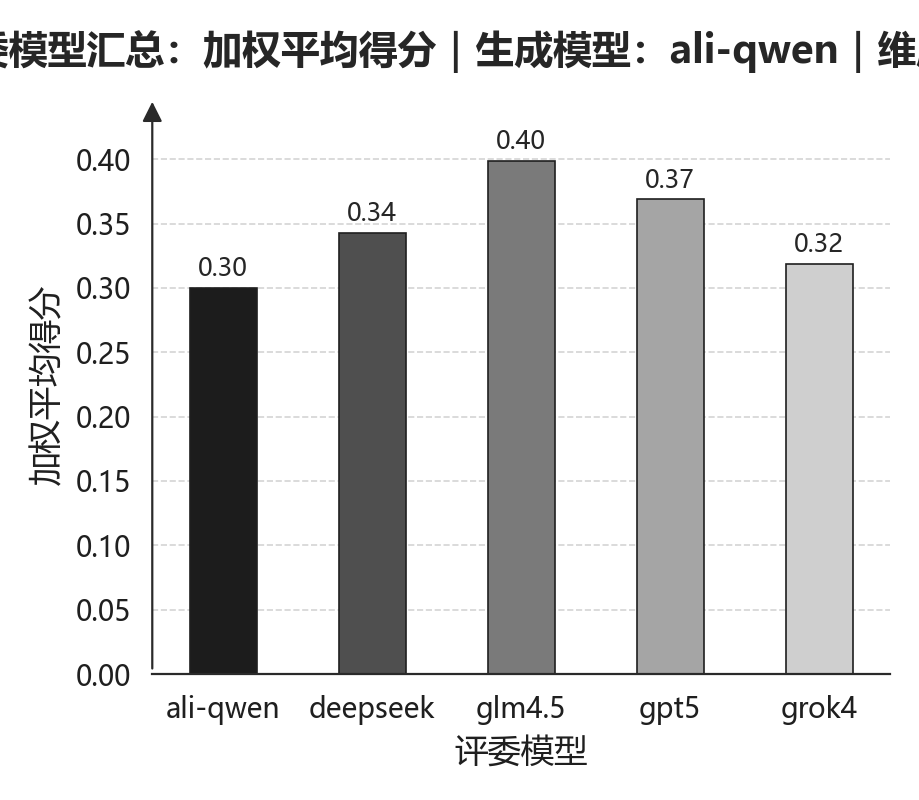
\includegraphics[width=0.95\textwidth]{images/plots/有效性/generator/ali-qwen/generator_bar_by_judge_ali-qwen_有效性.png}}\\
	 \subfloat[\texttt{DeepSeek}\label{fig:app-eff-generator-by-judge-deepseek}]{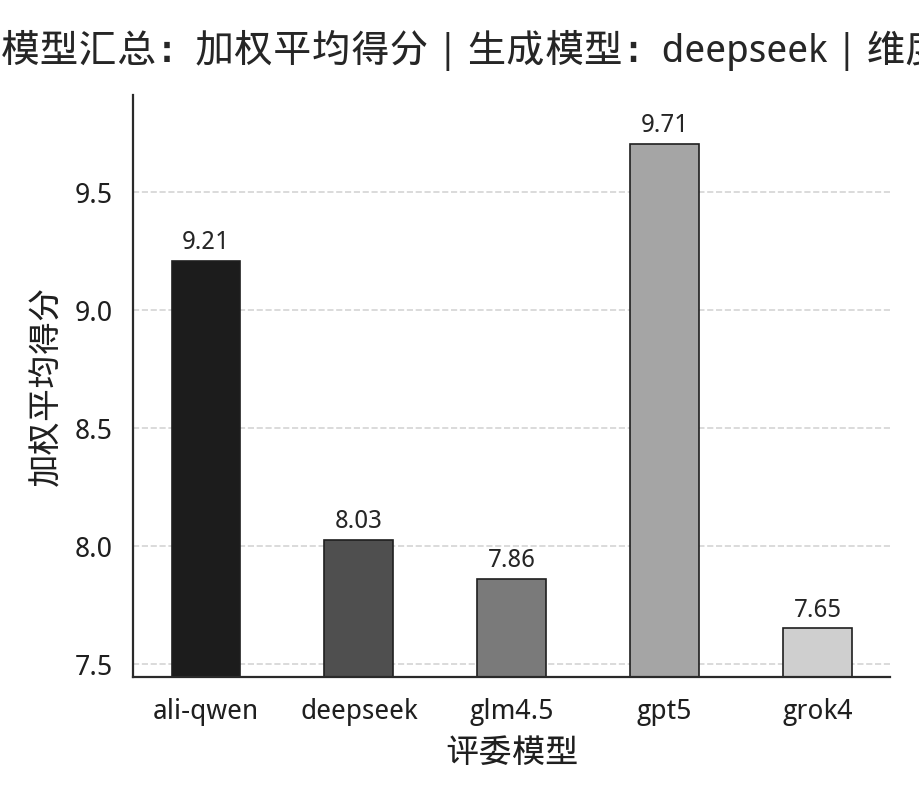
\includegraphics[width=0.95\textwidth]{images/plots/有效性/generator/deepseek/generator_bar_by_judge_deepseek_有效性.png}}\\
	 \subfloat[\texttt{GPT-5}\label{fig:app-eff-generator-by-judge-gpt5}]{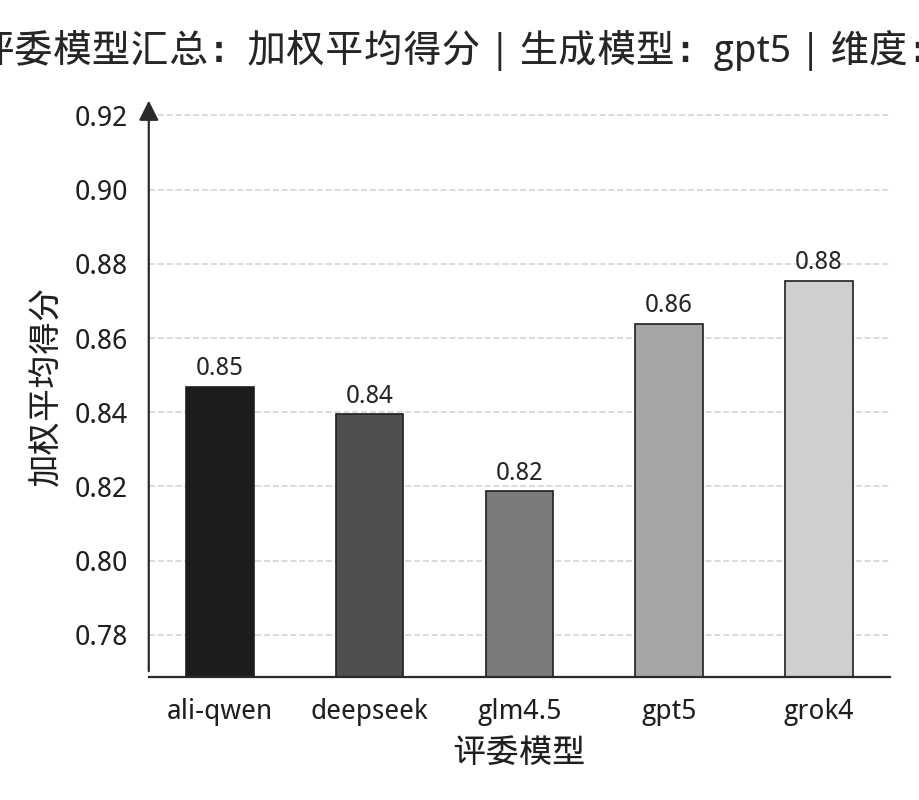
\includegraphics[width=0.95\textwidth]{images/plots/有效性/generator/gpt5/generator_bar_by_judge_gpt5_有效性.png}}}
	\caption{有效性维度下，不同生成模型在各评审模型下的排名式评分对照（I）。}\label{fig:app-eff-generator-by-judge}
\end{figure}

\begin{figure}[!ht]
	\centering
	{\setlength{\abovecaptionskip}{2pt}%
	 \setlength{\belowcaptionskip}{0pt}%
	 \subfloat[\texttt{Grok}\label{fig:app-eff-generator-by-judge-grok}]{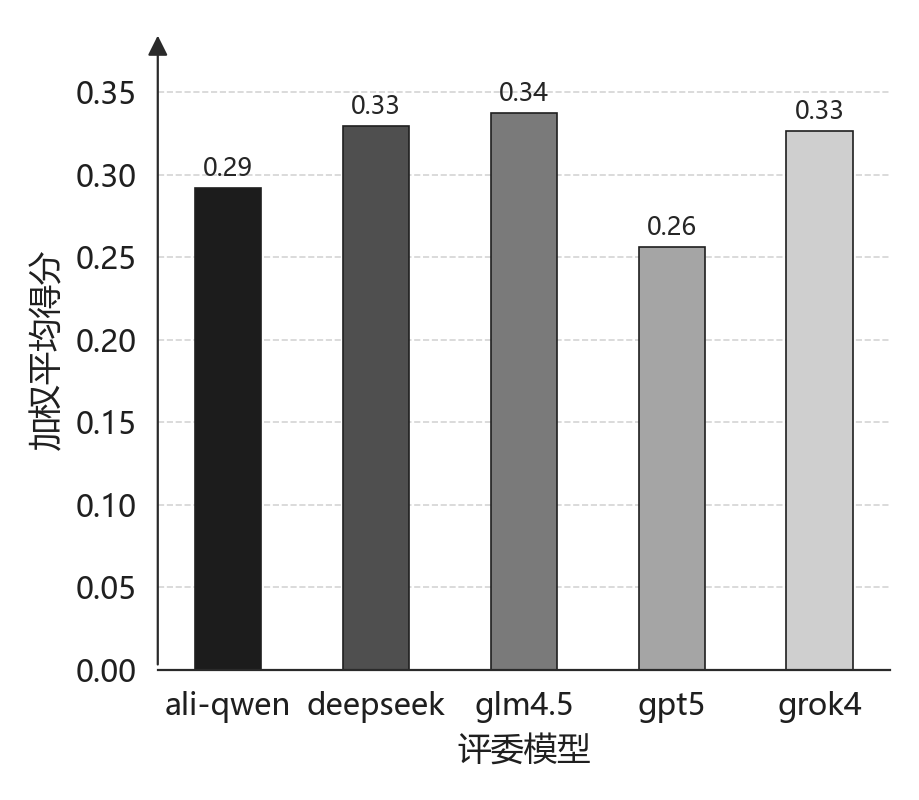
\includegraphics[width=0.95\textwidth]{images/plots/有效性/generator/grok4/generator_bar_by_judge_grok4_有效性.png}}\\
	 \subfloat[\texttt{GLM-4.6}\label{fig:app-eff-generator-by-judge-glm46}]{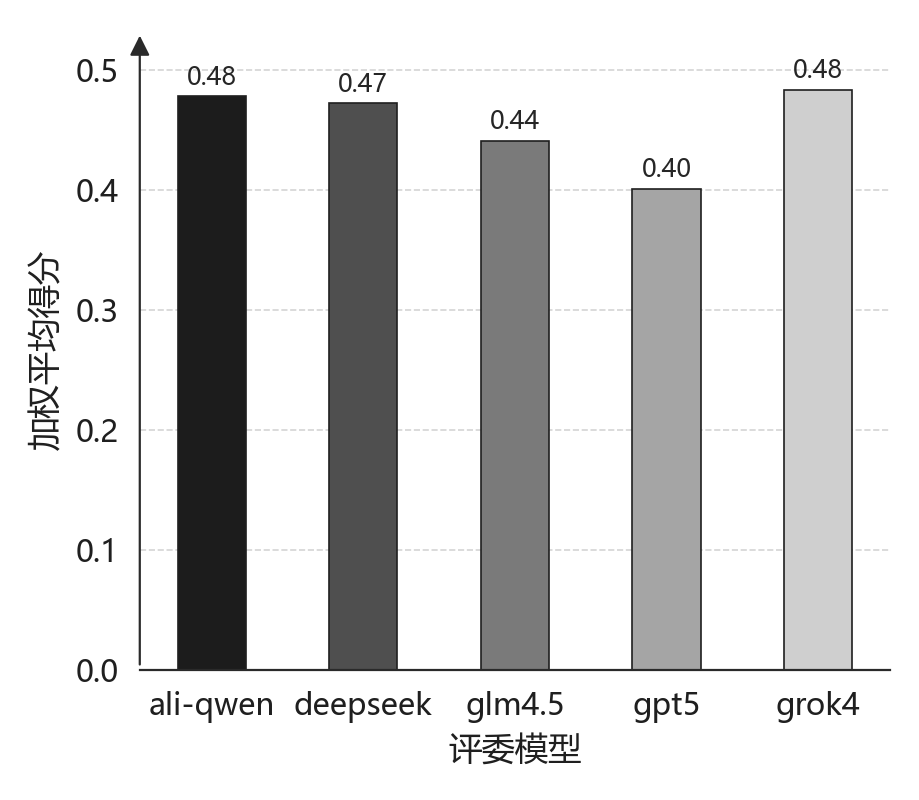
\includegraphics[width=0.95\textwidth]{images/plots/有效性/generator/glm4.5/generator_bar_by_judge_glm4.5_有效性.png}}}
	\caption{有效性维度下，不同生成模型在各评审模型下的排名式评分对照（II）。}\label{fig:app-eff-generator-by-judge-cont}
\end{figure}

\subsection{不同生成模型的结构性对照（热力图）}
\begin{figure}[!ht]
	\centering
	{\setlength{\abovecaptionskip}{2pt}%
	 \setlength{\belowcaptionskip}{0pt}%
	 \subfloat[\texttt{Qwen3}\label{fig:app-eff-heatmap-generator-qwen3}]{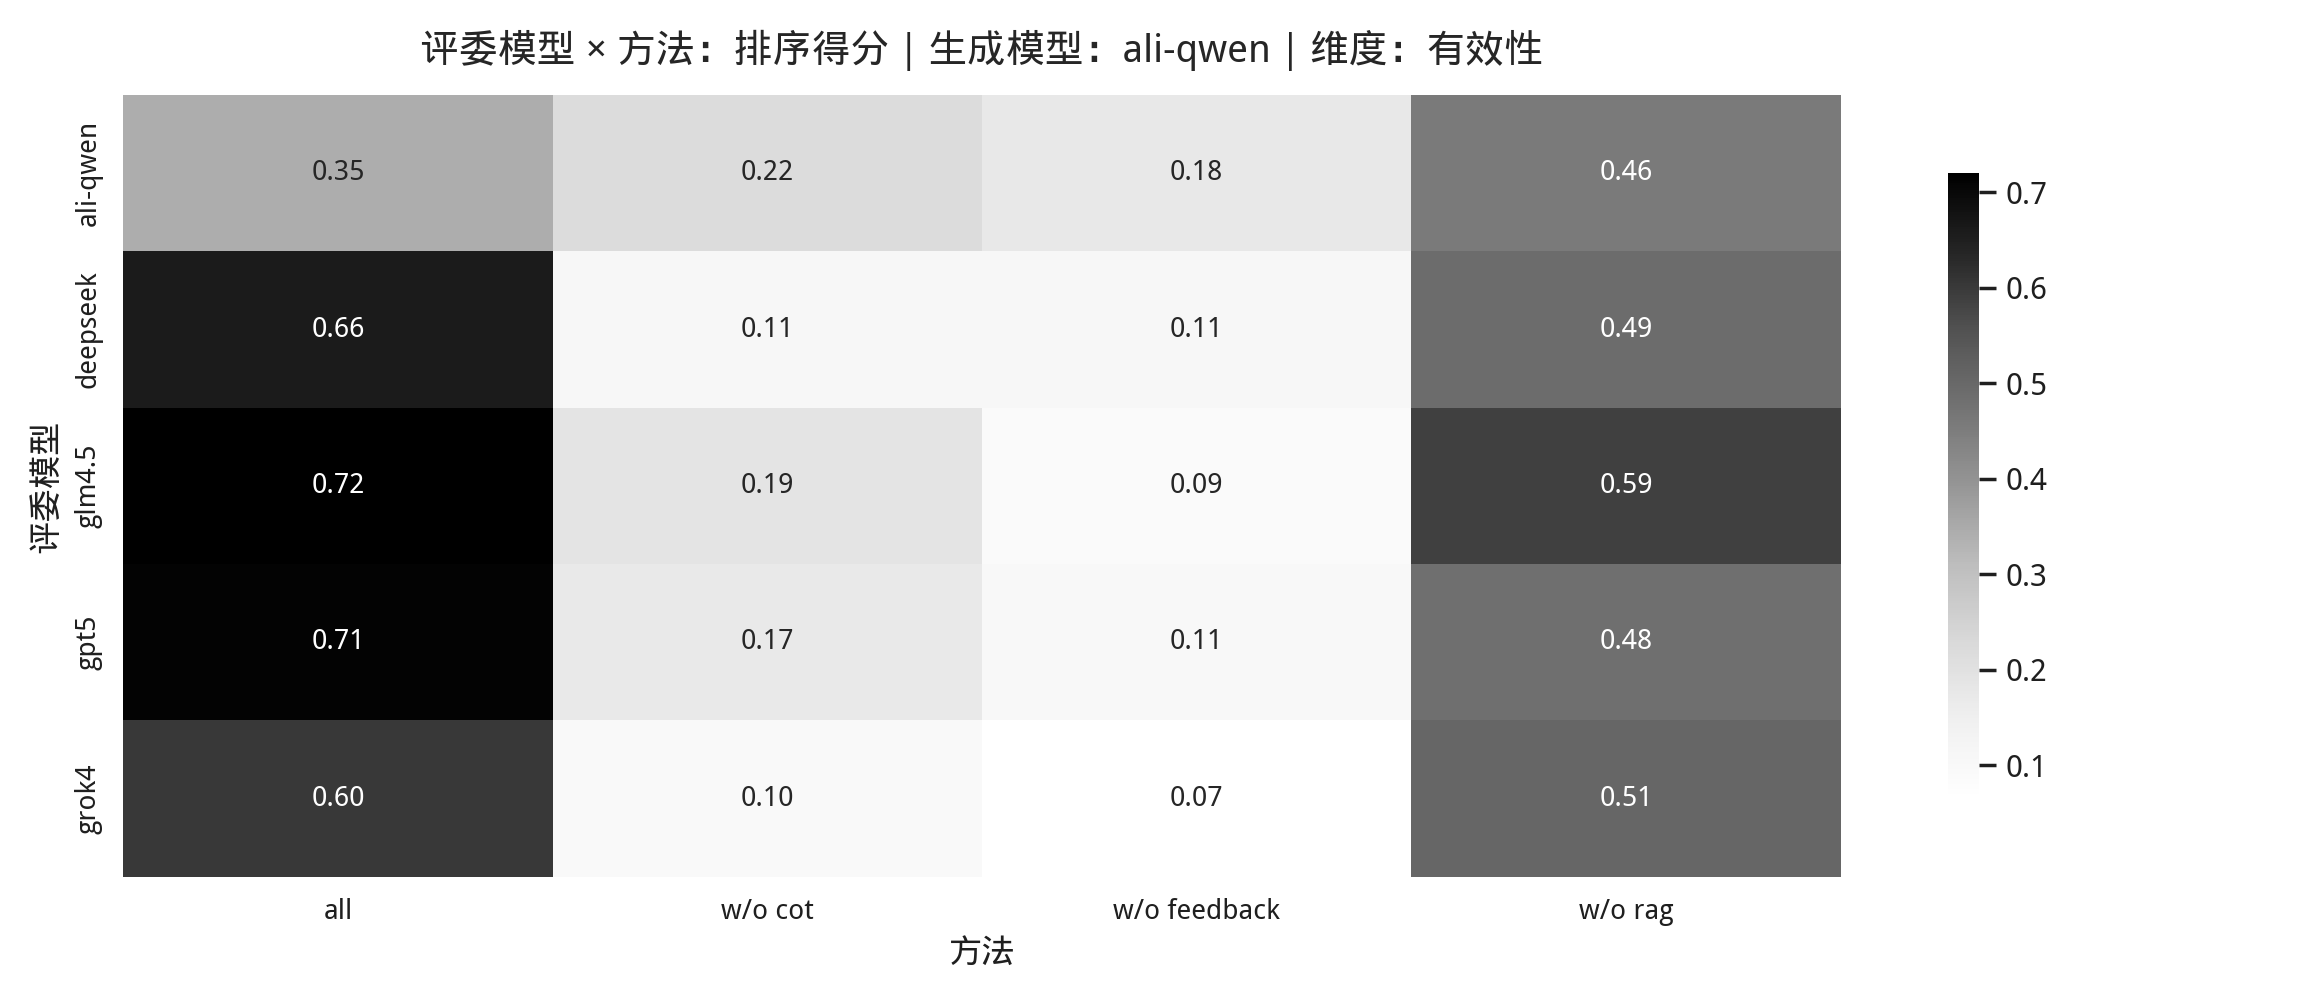
\includegraphics[width=0.95\textwidth]{images/plots/有效性/generator/ali-qwen/heatmap_generator_ali-qwen_有效性.png}}\\
	 \subfloat[\texttt{DeepSeek}\label{fig:app-eff-heatmap-generator-deepseek}]{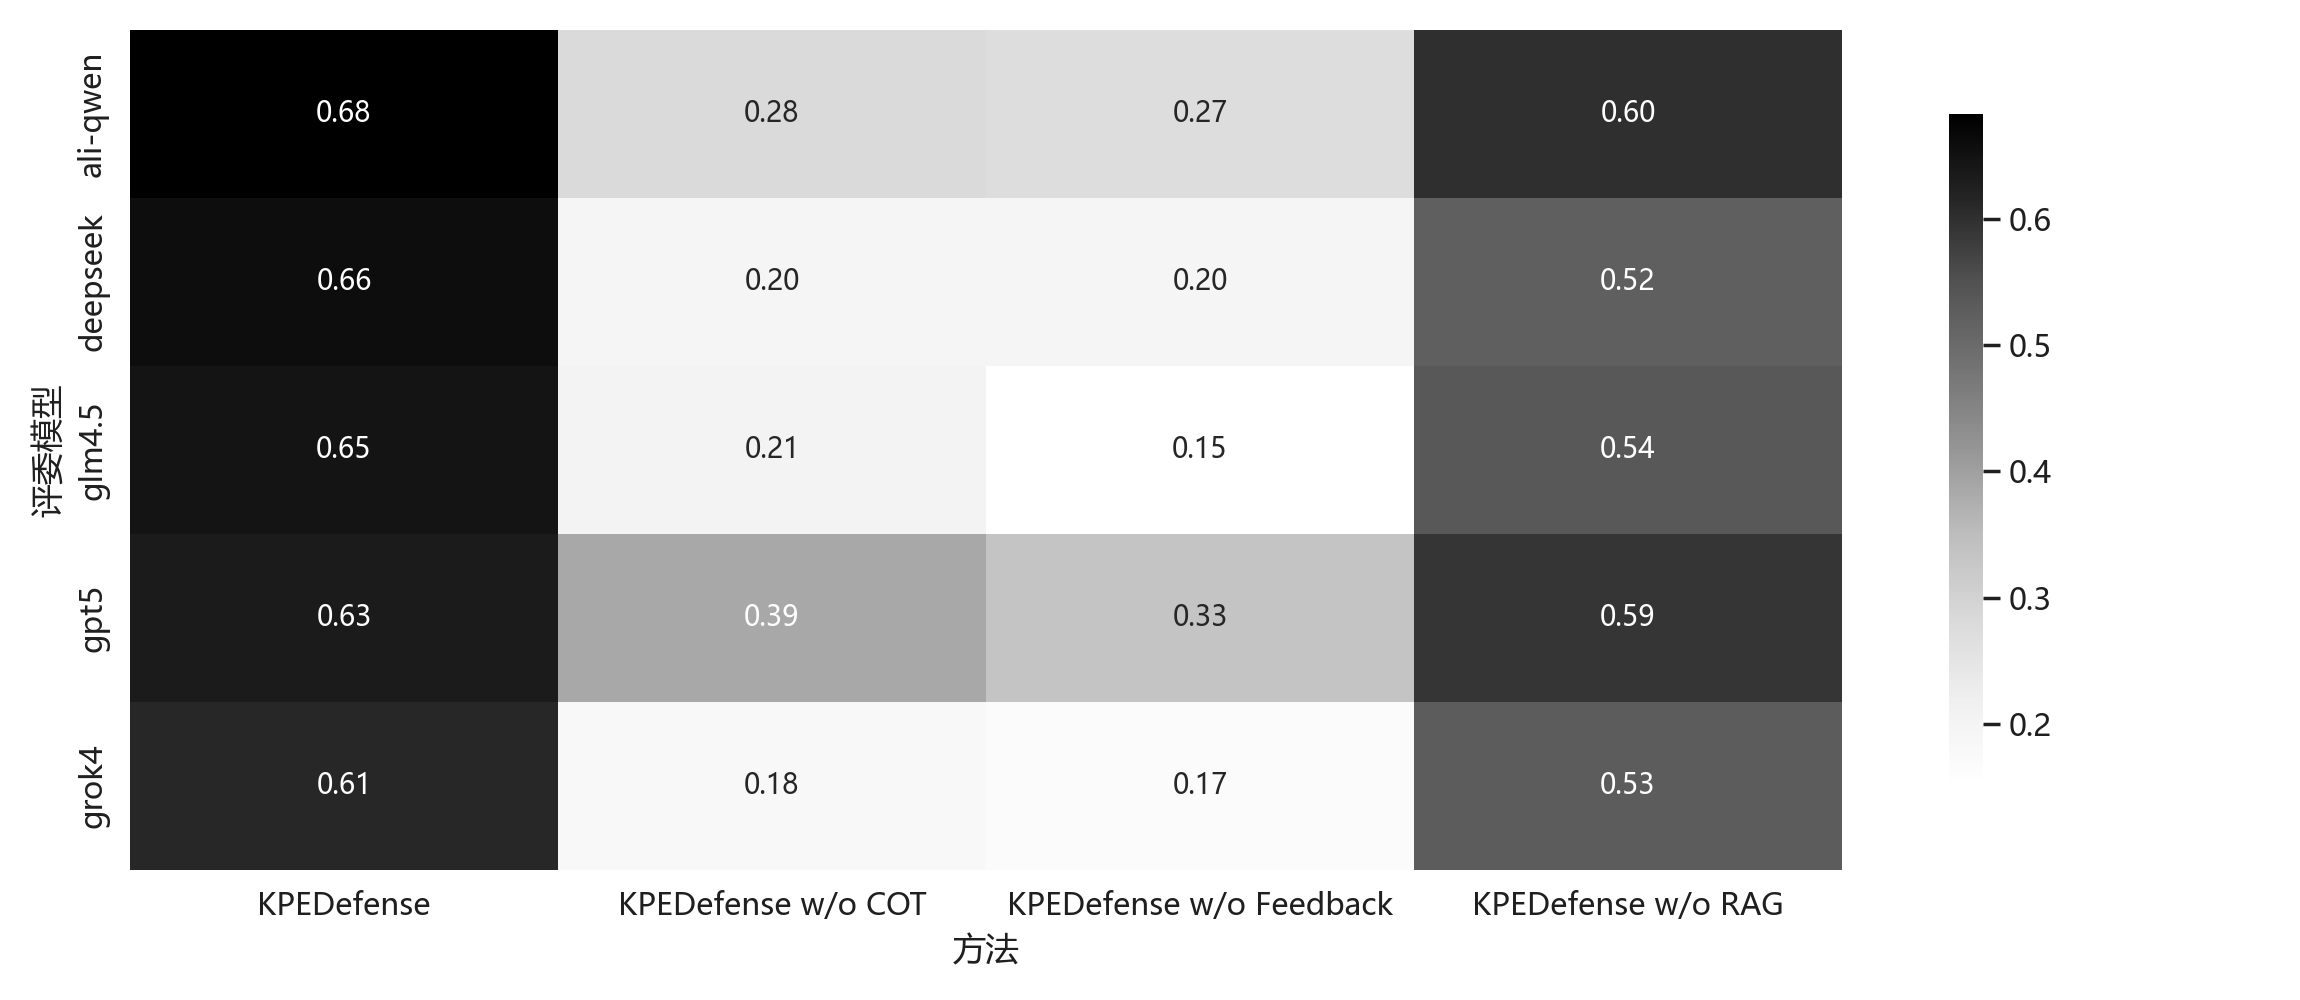
\includegraphics[width=0.95\textwidth]{images/plots/有效性/generator/deepseek/heatmap_generator_deepseek_有效性.png}}\\
	 \subfloat[\texttt{GPT-5}\label{fig:app-eff-heatmap-generator-gpt5}]{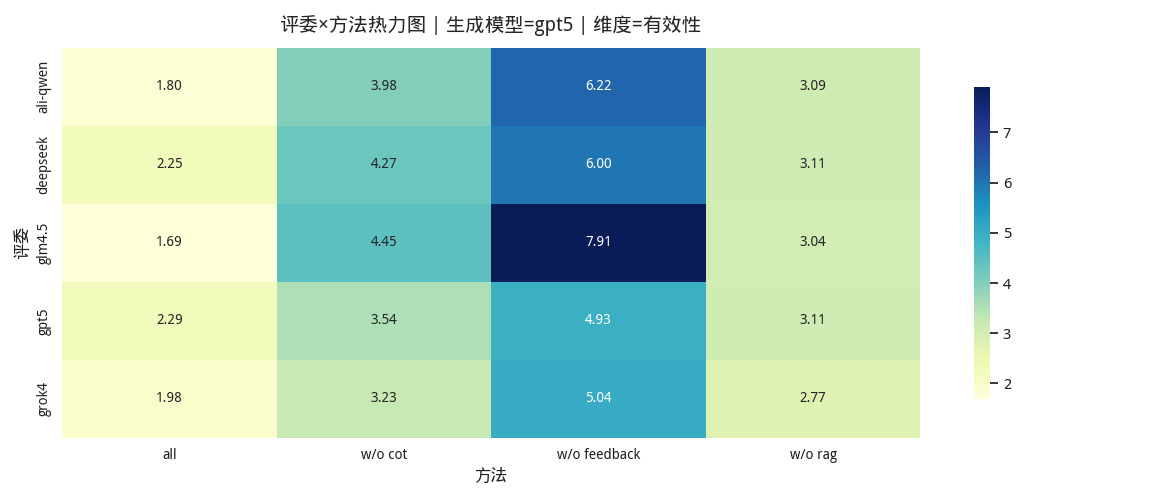
\includegraphics[width=0.95\textwidth]{images/plots/有效性/generator/gpt5/heatmap_generator_gpt5_有效性.png}}}
	\caption{有效性维度下，不同生成模型的结构性热力图对照（I）。}\label{fig:app-eff-heatmap-generator}
\end{figure}

\begin{figure}[!ht]
	\centering
	{\setlength{\abovecaptionskip}{2pt}%
	 \setlength{\belowcaptionskip}{0pt}%
	 \subfloat[\texttt{Grok}\label{fig:app-eff-heatmap-generator-grok}]{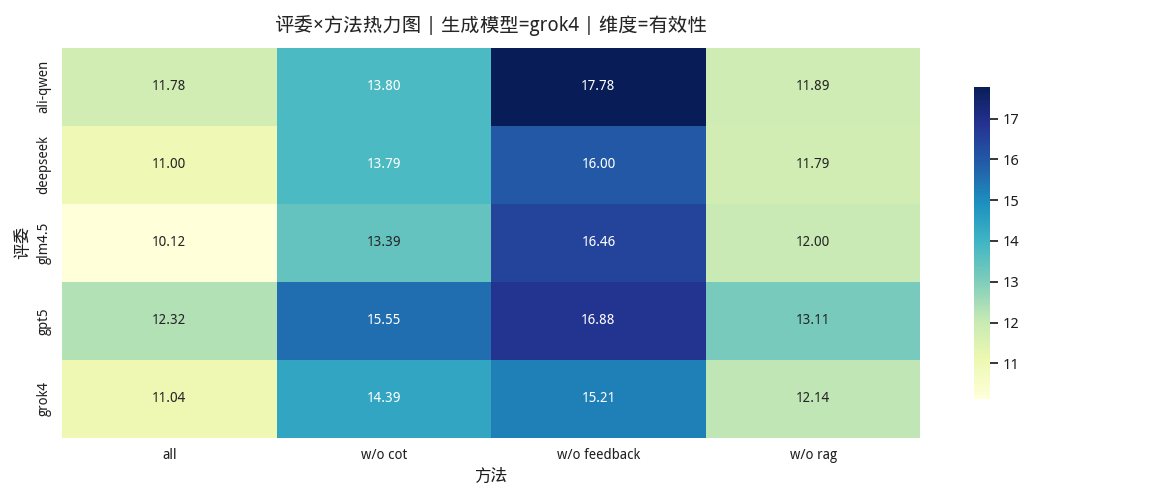
\includegraphics[width=0.95\textwidth]{images/plots/有效性/generator/grok4/heatmap_generator_grok4_有效性.png}}\\
	 \subfloat[\texttt{GLM-4.6}\label{fig:app-eff-heatmap-generator-glm46}]{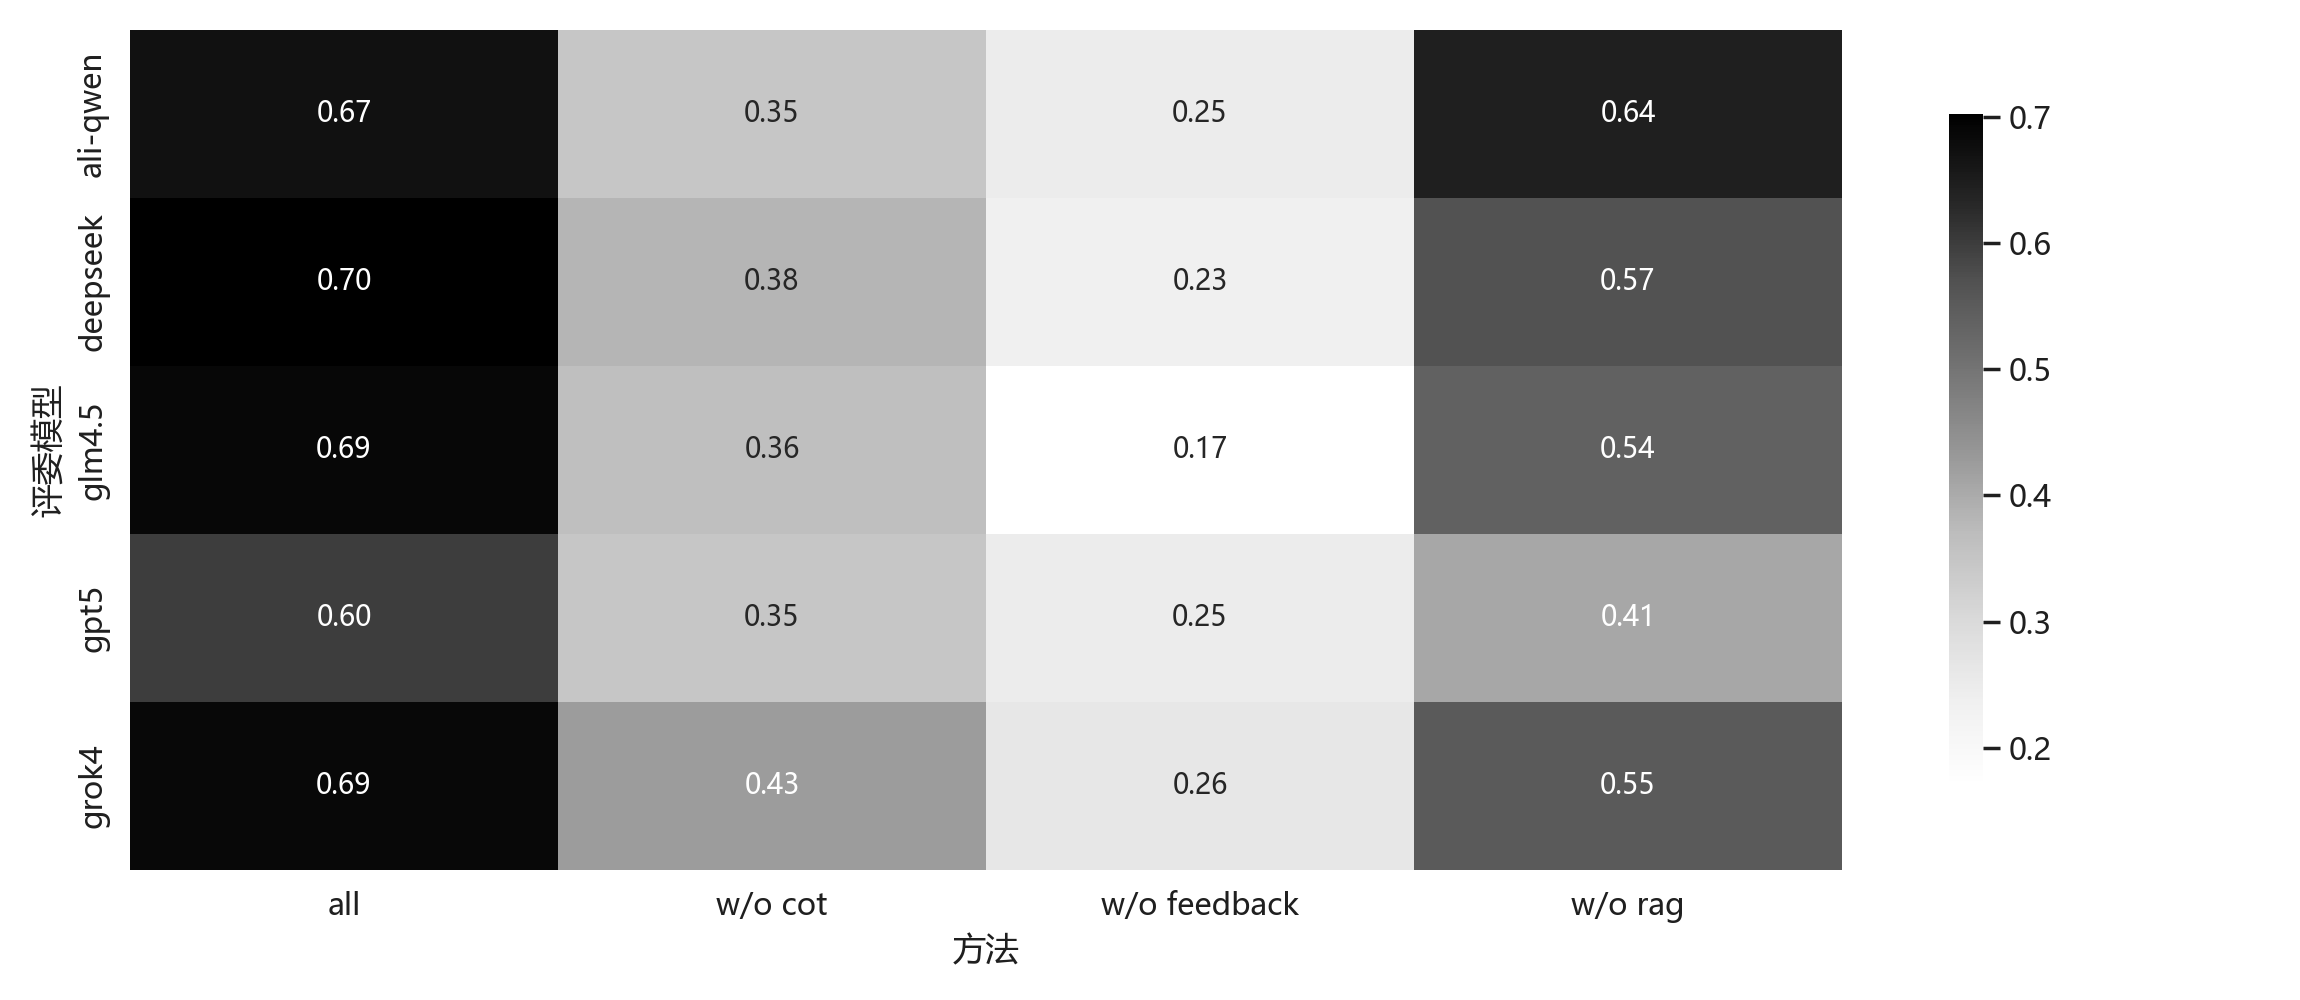
\includegraphics[width=0.95\textwidth]{images/plots/有效性/generator/glm4.5/heatmap_generator_glm4.5_有效性.png}}}
	\caption{有效性维度下，不同生成模型的结构性热力图对照（II）。}\label{fig:app-eff-heatmap-generator-cont}
\end{figure}

\section{可部署性：补充图表}\label{app:plots-deployability}

\subsection{按生成模型拆分的热力图（评审偏好结构）}
\begin{figure}[!ht]
	\centering
	{\setlength{\abovecaptionskip}{2pt}%
	 \setlength{\belowcaptionskip}{0pt}%
	 \subfloat[\texttt{Qwen3}\label{fig:app-deploy-heatmap-qwen3}]{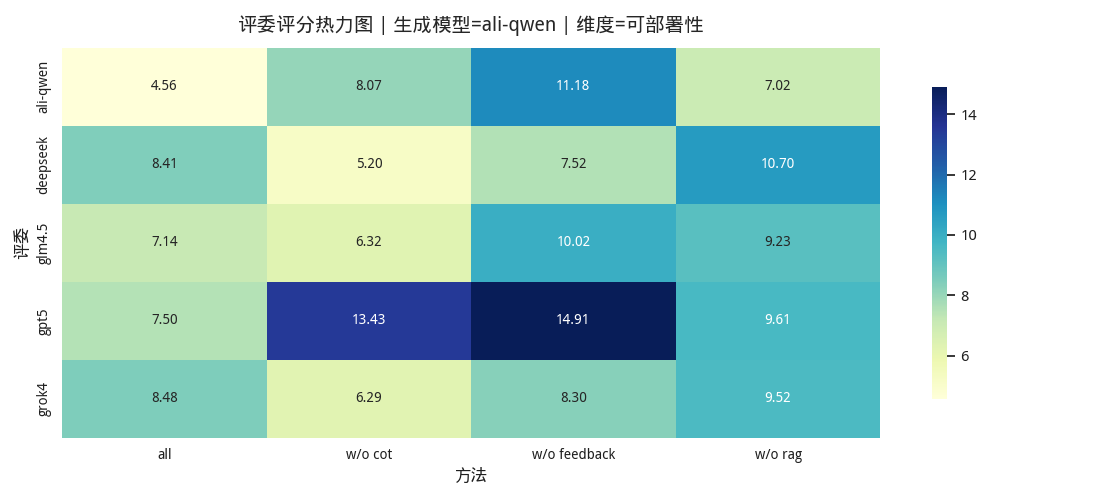
\includegraphics[width=0.95\textwidth]{images/plots/可部署性/heatmap/ali-qwen/heatmap_ali-qwen_可部署性.png}}\\
	 \subfloat[\texttt{DeepSeek}\label{fig:app-deploy-heatmap-deepseek}]{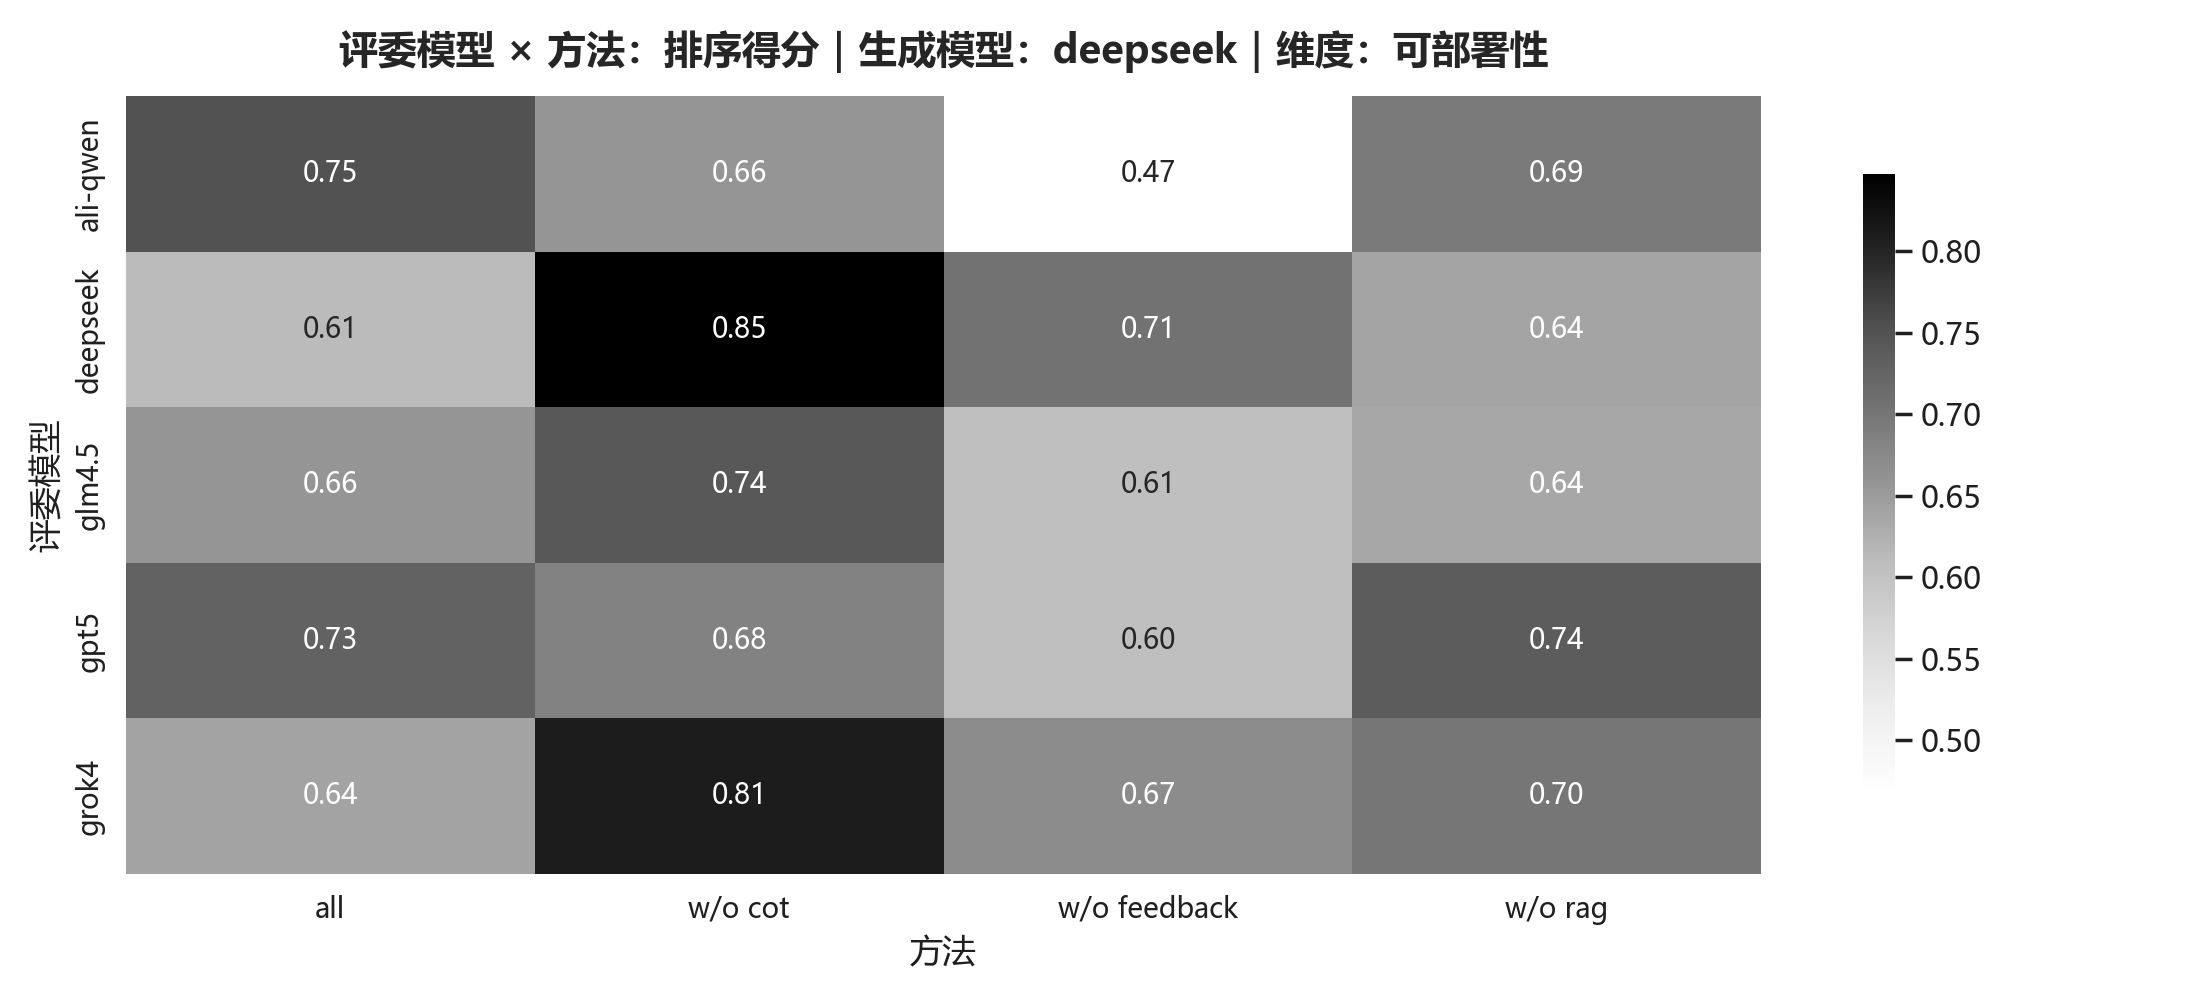
\includegraphics[width=0.95\textwidth]{images/plots/可部署性/heatmap/deepseek/heatmap_deepseek_可部署性.png}}\\
	 \subfloat[\texttt{GPT-5}\label{fig:app-deploy-heatmap-gpt5}]{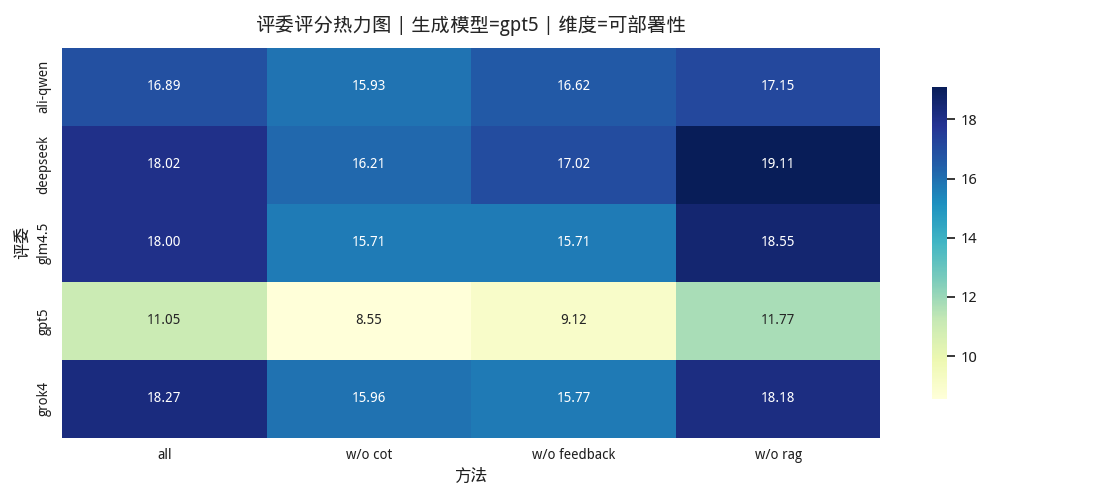
\includegraphics[width=0.95\textwidth]{images/plots/可部署性/heatmap/gpt5/heatmap_gpt5_可部署性.png}}}
	\caption{可部署性维度下，不同评审模型的偏好结构热力图对照（I）。}\label{fig:app-deploy-heatmap}
\end{figure}

\begin{figure}[!ht]
	\centering
	{\setlength{\abovecaptionskip}{2pt}%
	 \setlength{\belowcaptionskip}{0pt}%
	 \subfloat[\texttt{Grok}\label{fig:app-deploy-heatmap-grok}]{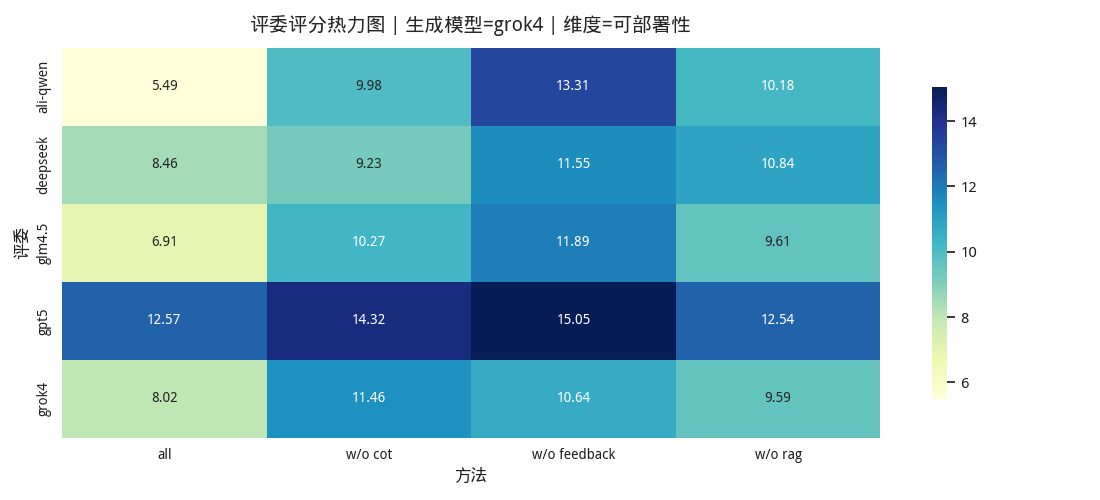
\includegraphics[width=0.95\textwidth]{images/plots/可部署性/heatmap/grok4/heatmap_grok4_可部署性.png}}\\
	 \subfloat[\texttt{GLM-4.6}\label{fig:app-deploy-heatmap-glm46}]{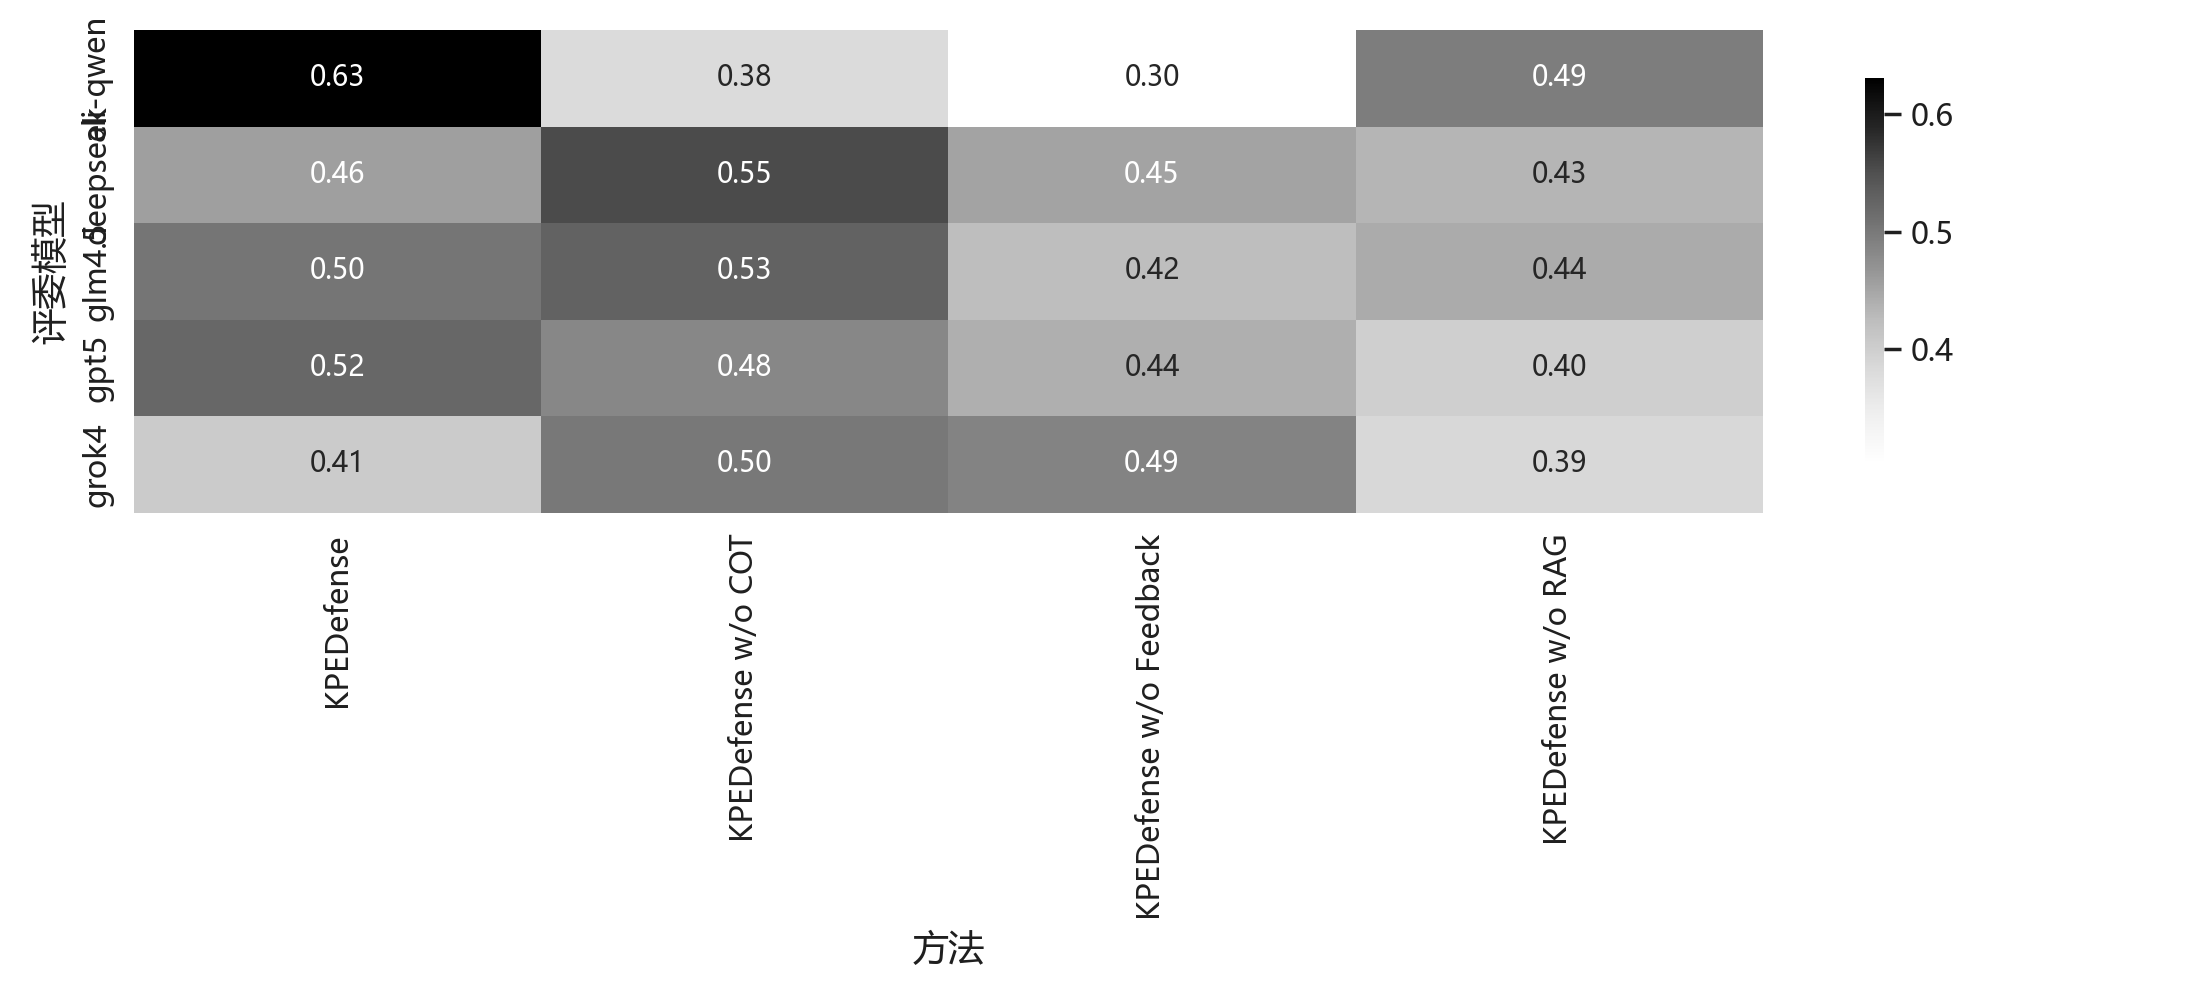
\includegraphics[width=0.95\textwidth]{images/plots/可部署性/heatmap/glm4.5/heatmap_glm4.5_可部署性.png}}}
	\caption{可部署性维度下，不同评审模型的偏好结构热力图对照（II）。}\label{fig:app-deploy-heatmap-cont}
\end{figure}

\section{无干扰性：补充图表}\label{app:plots-interference}

\subsection{按生成模型拆分的热力图（评审偏好结构）}
\begin{figure}[!ht]
	\centering
	{\setlength{\abovecaptionskip}{2pt}%
	 \setlength{\belowcaptionskip}{0pt}%
	 \subfloat[\texttt{Qwen3}\label{fig:app-interf-heatmap-qwen3}]{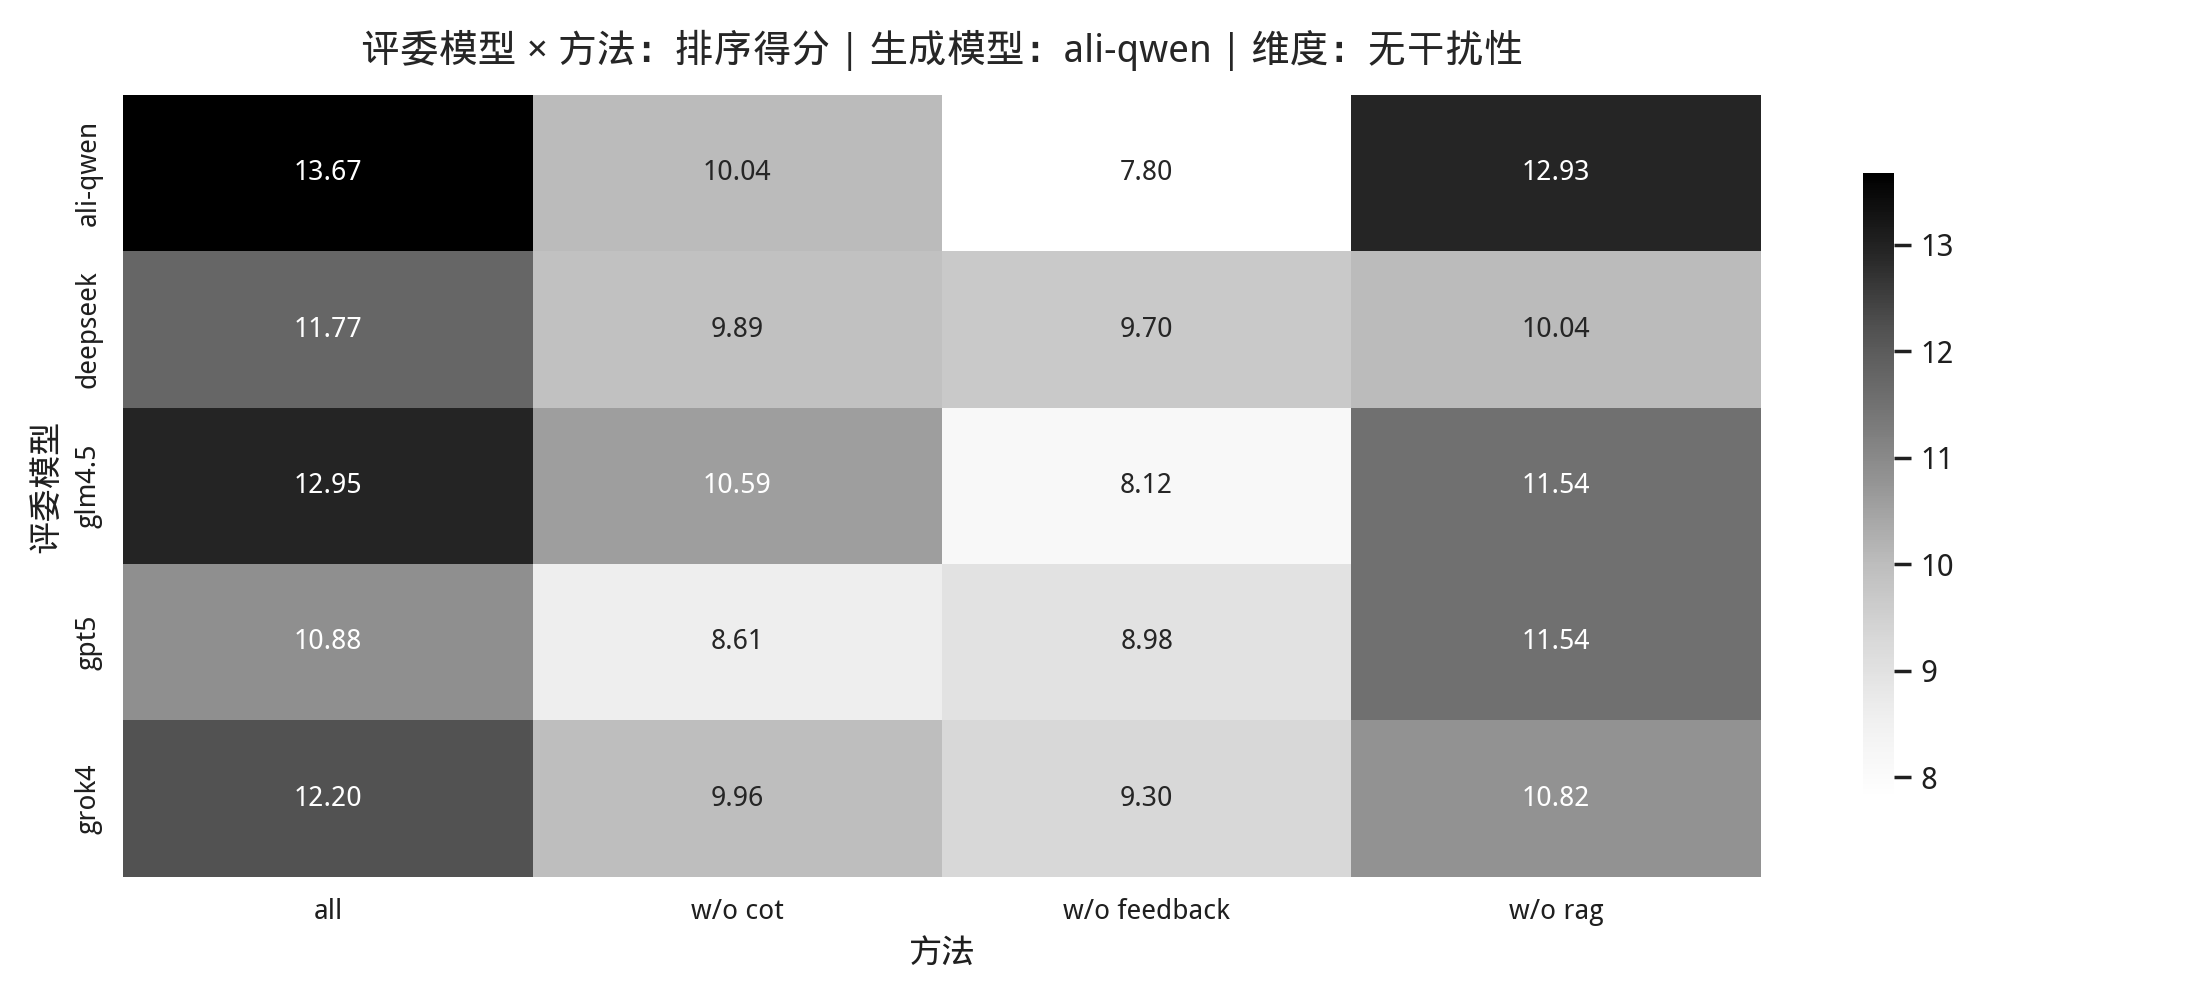
\includegraphics[width=0.95\textwidth]{images/plots/无干扰性/heatmap/ali-qwen/heatmap_ali-qwen_无干扰性.png}}\\
	 \subfloat[\texttt{DeepSeek}\label{fig:app-interf-heatmap-deepseek}]{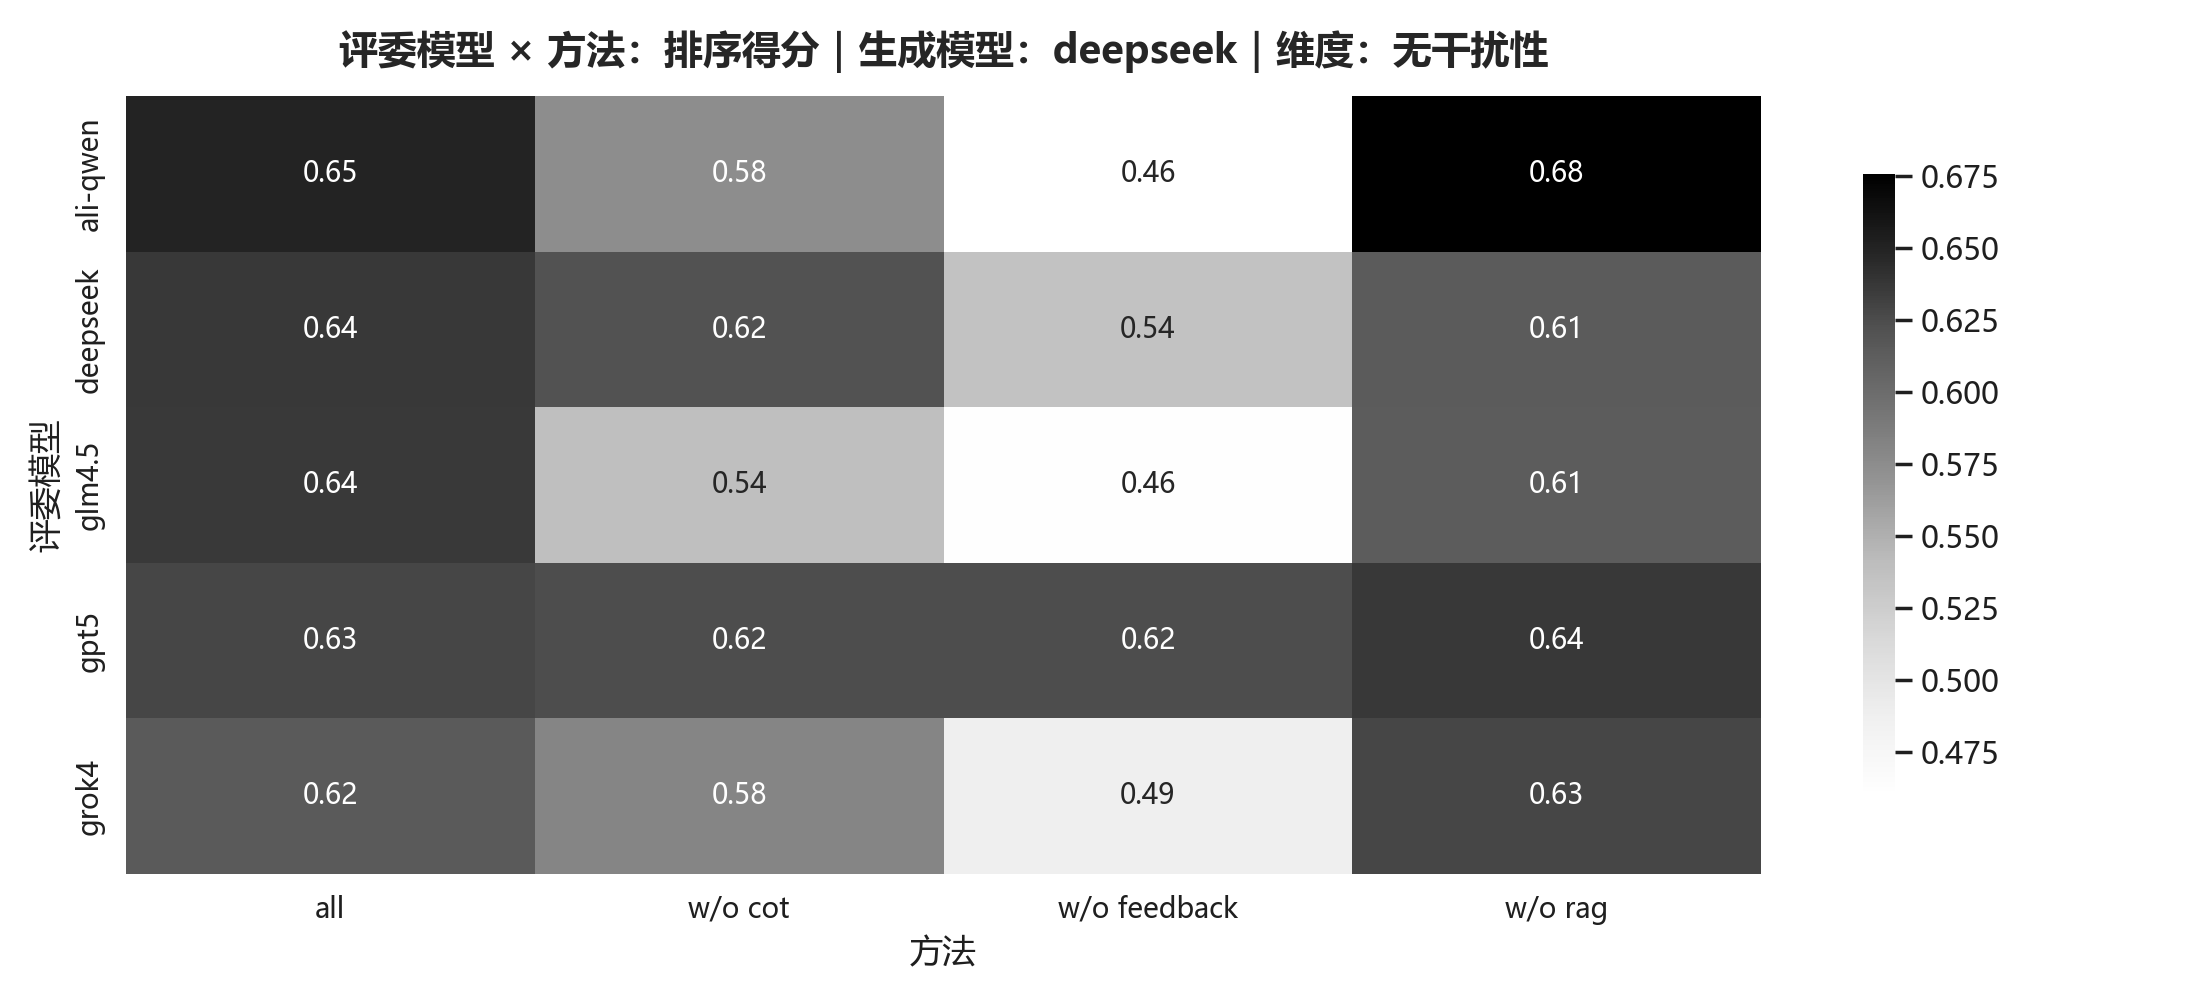
\includegraphics[width=0.95\textwidth]{images/plots/无干扰性/heatmap/deepseek/heatmap_deepseek_无干扰性.png}}\\
	 \subfloat[\texttt{GPT-5}\label{fig:app-interf-heatmap-gpt5}]{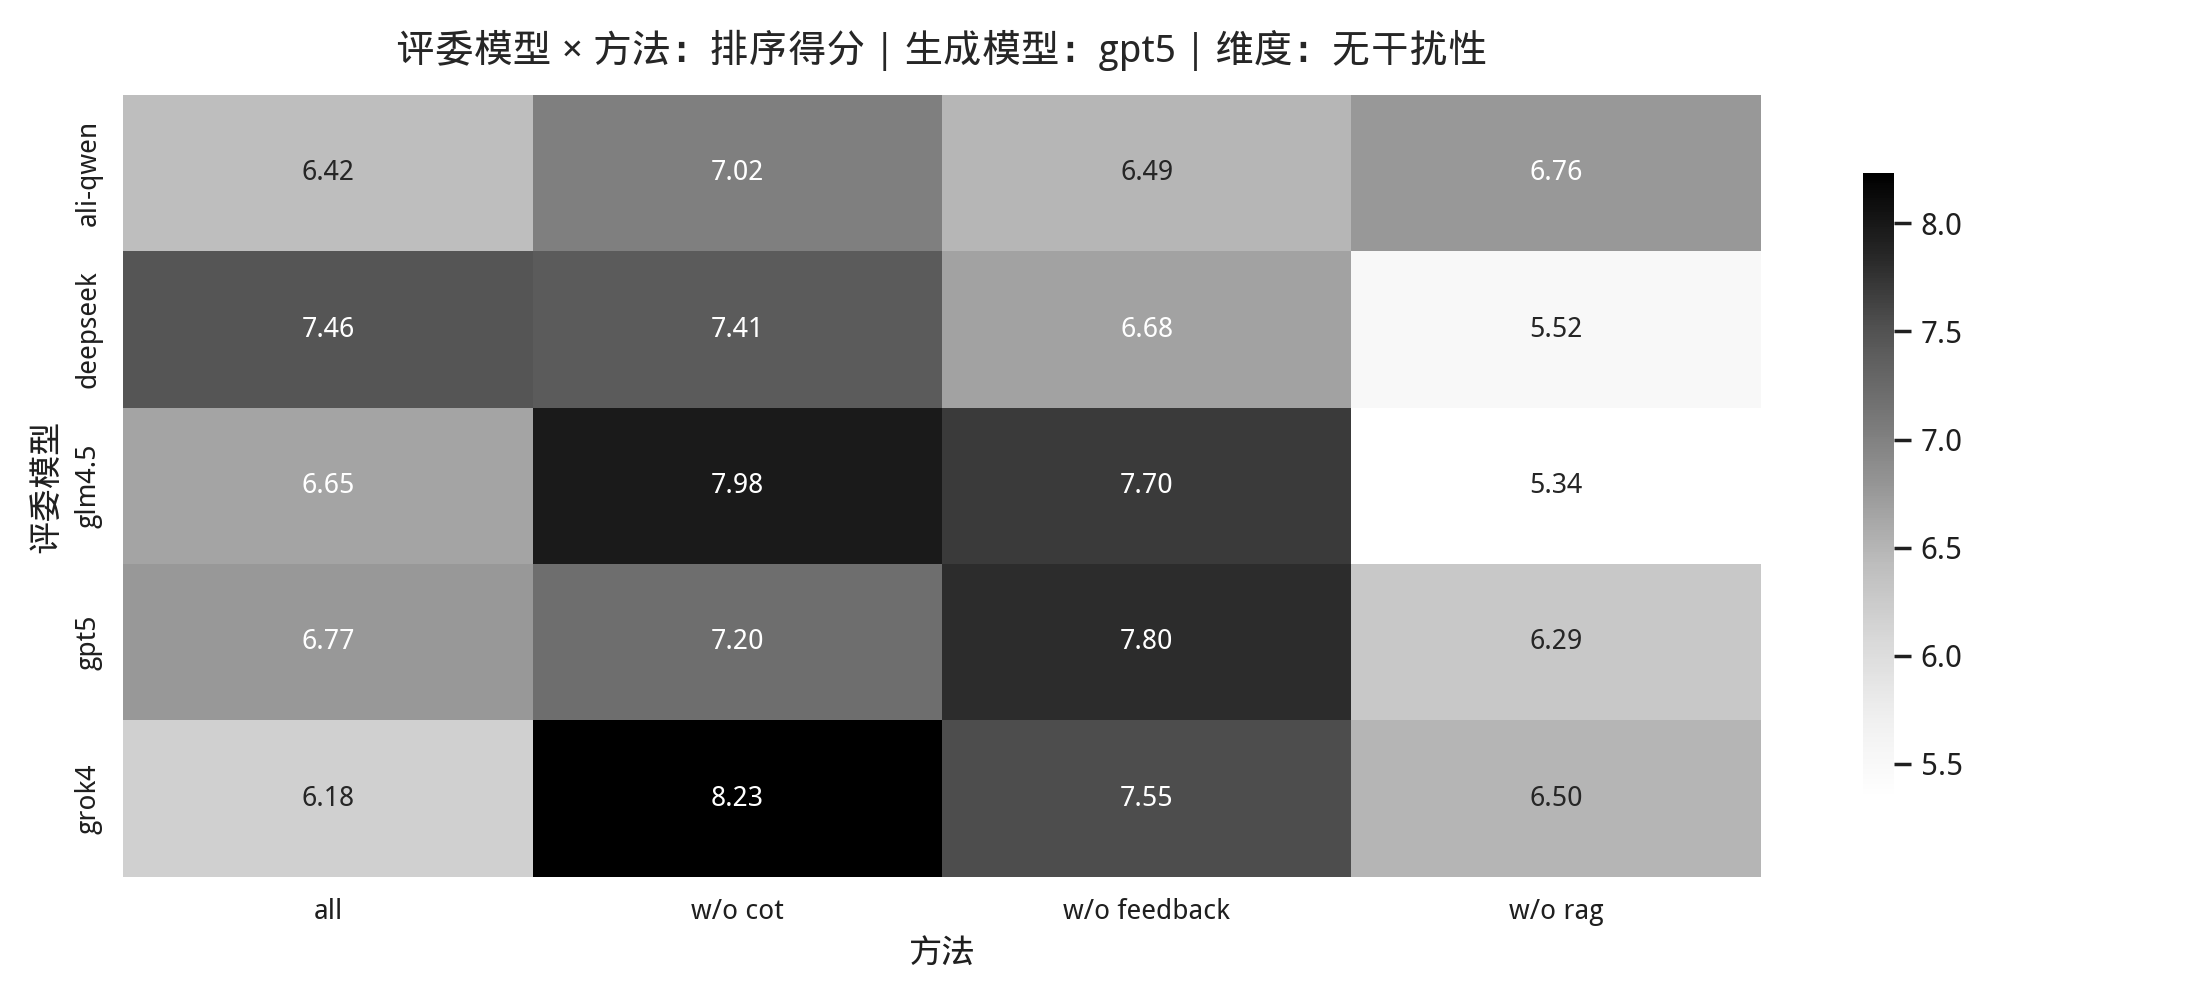
\includegraphics[width=0.95\textwidth]{images/plots/无干扰性/heatmap/gpt5/heatmap_gpt5_无干扰性.png}}}
	\caption{无干扰性维度下，不同评审模型的偏好结构热力图对照（I）。}\label{fig:app-interf-heatmap}
\end{figure}

\begin{figure}[!ht]
	\centering
	{\setlength{\abovecaptionskip}{2pt}%
	 \setlength{\belowcaptionskip}{0pt}%
	 \subfloat[\texttt{Grok}\label{fig:app-interf-heatmap-grok}]{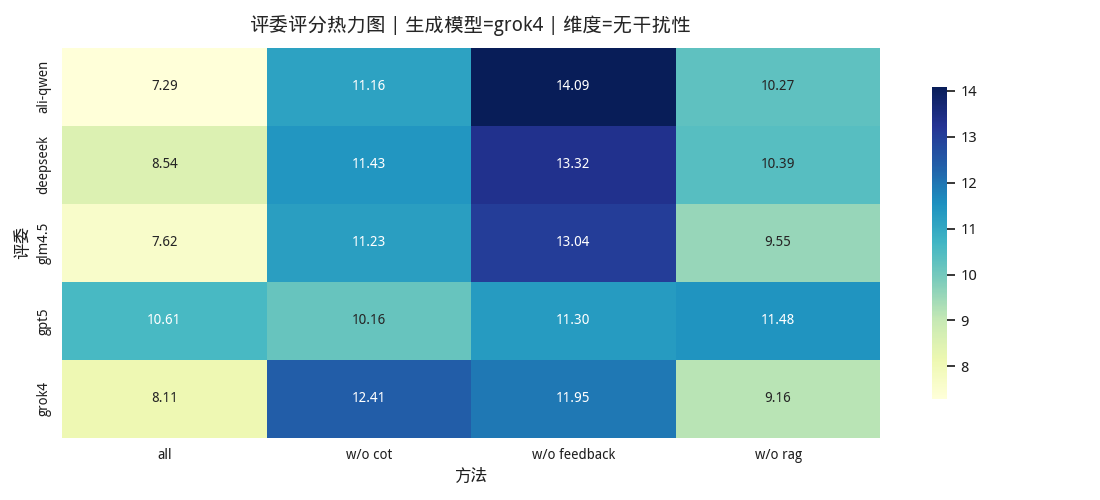
\includegraphics[width=0.95\textwidth]{images/plots/无干扰性/heatmap/grok4/heatmap_grok4_无干扰性.png}}\\
	 \subfloat[\texttt{GLM-4.6}\label{fig:app-interf-heatmap-glm46}]{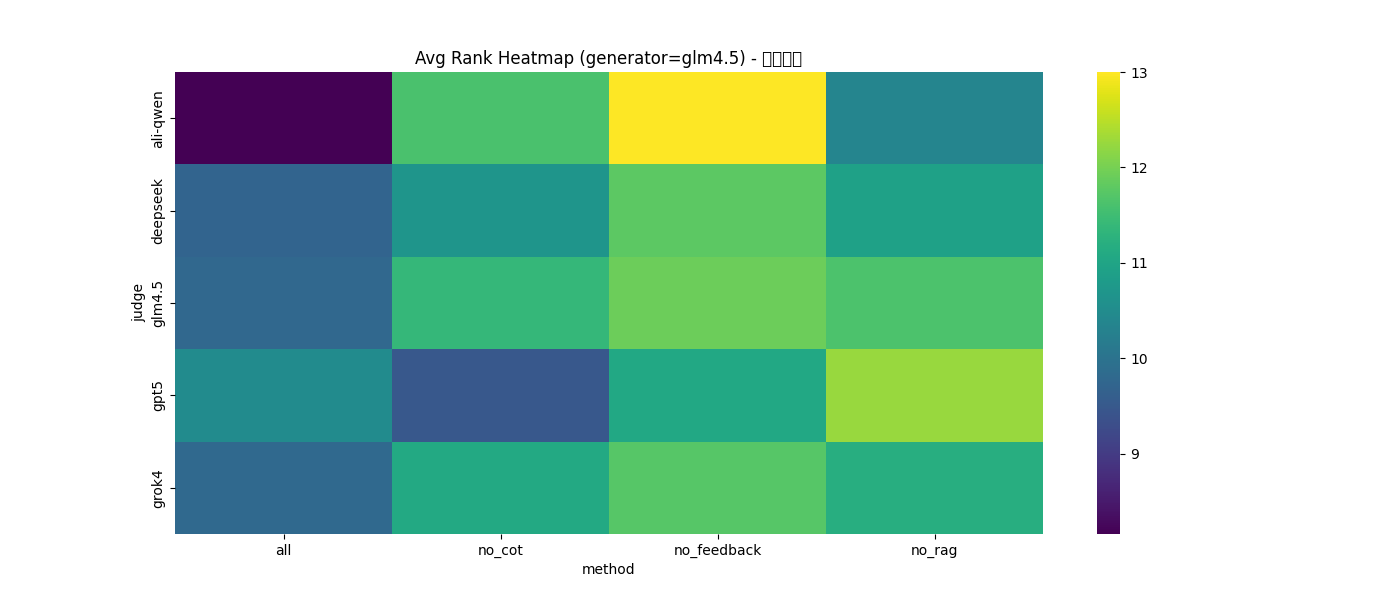
\includegraphics[width=0.95\textwidth]{images/plots/无干扰性/heatmap/glm4.5/heatmap_glm4.5_无干扰性.png}}}
	\caption{无干扰性维度下，不同评审模型的偏好结构热力图对照（II）。}\label{fig:app-interf-heatmap-cont}
\end{figure}
%% 致谢

%% 致谢
%\pagestyle{empty}
\chapter*{致\quad\quad 谢}%\addcontentsline{toc}{chapter}{致谢}

% 时光荏苒，岁月如梭。在导师的悉心指导和亲友的默默支持下，本论文终于得以顺利完成。值此定稿之际，我谨向所有在我的硕士学习和生活期间给予我帮助与支持的人，致以最诚挚的谢意。

% 首先，我要向我的导师本论文导师教授表达最衷心的感谢和崇高的敬意。在我的整个硕士学习阶段，从论文的选题、开题、研究工作的开展到最终的定稿，孙老师都倾注了大量的心血，给予了我悉心的指导。孙老师严谨的治学态度、渊博的专业知识以及对科研的热忱，使我受益匪浅，也将成为我今后工作和学习中的宝贵财富。

% 其次，感谢北京科技大学为我提供了良好的学习和科研环境。感谢在此期间教导过我的所有老师，感谢你们的传道授业解惑。我要特别感谢实验室的同门们以及我的室友。我们不仅在科研上互相切磋、共同进步，在日常生活中也彼此照应，让我的研究生时光充满了欢乐与温暖。

% 此外，我还要特别感谢在北京的各位高中同学和朋友们。在紧张的科研之余，是你们的陪伴与鼓励，给了我莫大的放松与慰藉，让我在求学之路上不觉孤单。

% 最后，我要深深感谢我的家人。正是你们多年如一日的默默付出、理解与无私的爱，为我撑起了一片充满温暖的天空，让我能够全心全意地投入到学业之中。你们永远是我最坚实的后盾和不断前行的最大动力。

% 感谢开源社区的所有贡献者们，你们的无私奉献和创新精神为我的研究提供了宝贵的资源和灵感。

% 感谢所有关心和帮助过我的人！


%% 作者简历及在学研究成果
\include{contents/mresume}
%% 关于论文使用授权的说明
\postDeclarations
%% 学位论文数据集
\chapter*{学位论文数据集}%\addcontentsline{toc}{chapter}{学位论文数据集}
\addcontentsline{toc}{chapter}{学位论文数据集}
\vskip16.5pt
\noindent\zihao{5}\begin{tabu} to \textwidth{|X|X|X|X|X|}
\hline
关键词* & 密级* & 中图分类号* & UDC & 论文资助 \\\hline
云原生安全；权限提升漏洞；策略代码生成；补丁窗口期监控与防护；多智能体协同 & 公开 & TP311 & 004.41 & H0251056\\\hline
\multicolumn2{|l|}{学位授予单位名称*} & {学位授予单位代码*} & 学位类别* & 学位级别* \\\hline
\multicolumn{2}{|l|}{北京科技大学}&10008  & 工学 & 硕士 \\\hline
\multicolumn2{|l|}{论文题名*} & \multicolumn2{|l|}{并列题名} & 论文语种* \\\hline
\multicolumn2{|l|}{\shortstack[l]{面向云原生应用权限提升漏洞的\\智能化防控技术研究}} & \multicolumn2{|l|}{} & 中文\\ \hline
作者姓名*&\multicolumn{2}{l|}{韩晓阳} & 学号* & M202310652 \\\hline
\multicolumn2{|l|}{培养单位名称*} & 培养单位代码* & 培养单位地址 & 邮编 \\\hline
\multicolumn2{|l|}{北京科技大学} & 10008 & 北京市海淀区学院路30号 & 100083\\\hline
\multicolumn2{|l|}{学科专业*} & 研究方向* & 学制* & 学位授予年* \\\hline
\multicolumn2{|l|}{计算机科学与技术} & 软件工程 & 3年 & 2026 \\\hline
论文提交日期* & \multicolumn4{l|}{2026 年 06 月 01 日} \\\hline
导师姓名*&\multicolumn2{l|}{孙昌爱} & 职称* & 教授 \\\hline
评阅人 &答辩委员会主席* & \multicolumn3{l|}{答辩委员会成员} \\\hline
& 阿孜古丽& \multicolumn3{l|}{邢博文} \\
& & \multicolumn3{l|}{郭茜} \\\hline
\multicolumn5{|l|}{电子版论文提交格式  文本（√）  图像（\, ） 视频（\, ） 音频（\, ） 多媒体（\, ） 其他（\, ）}\\
\multicolumn5{|l|}{推荐格式：application/msword; application/pdf} \\\hline
\multicolumn2{|l}{电子论文出版（发布）者} & \multicolumn2{|l|}{电子论文出版（发布）地} & 权限声明　\\\hline
\multicolumn2{|l|}{} & \multicolumn2{|l|}{} & \\\hline
论文总页数* & \multicolumn4{l|}{101} \\\hline
\multicolumn5{|l|}{共33项，其中带*为必填数据，为22项。}\\\hline
\end{tabu}


\end{document}
